%You can delete all the comments after you have finished your document
%this sets up the defaults for the documents, 12pt font and A4 size. The article type sets this up as such as opposed to letter or memo.

%for the finer points LaTeX see https://en.wikibooks.org/wiki/LaTeX or http://tex.stackexchange.com/

\documentclass[12pt,a4paper]{article}

%\usepackage{natbib}
\usepackage[style=apa,backend=biber,natbib=true,doi=false,isbn=false,url=true,eprint=false,hyperref=true]{biblatex} 
\addbibresource{references.bib}
\setlength\bibitemsep{\baselineskip}

\usepackage{titlesec} 
\usepackage{fancyhdr}

% !TEX TS-program = pdflatex
% !TEX encoding = UTF-8 Unicode
\usepackage[utf8]{inputenc} % set input encoding (not needed with XeLaTeX)
\usepackage[english]{babel}

\usepackage{graphicx} % support the \includegraphics command and options
\graphicspath{{./images/}}

\usepackage[subfigure,titles]{tocloft}                  
\usepackage[parfill]{parskip} % Activate to begin paragraphs with an empty line rather than an indent
% make citations clickable links, and change link colours to black
\usepackage[hidelinks,breaklinks,colorlinks,linkcolor={black},citecolor={black},urlcolor={black}]{hyperref}
\usepackage{tabularx,dcolumn}
\usepackage{longtable, booktabs, tabu} % for much better looking tables
\usepackage{array} % for better arrays (eg matrices) in maths
\usepackage{paralist} % very flexible & customisable lists (eg. enumerate/itemize, etc.)
\usepackage{verbatim} % adds environment for commenting out blocks of text & for better verbatim
\usepackage{subfig} % make it possible to include more than one captioned figure/table in a single float
\usepackage[toc,page]{appendix}
\usepackage{xargs} % Use more than one optional parameter in a new command
\usepackage[dvipsnames,table,xcdraw]{xcolor}
% break links on hyphens!
%\usepackage[hyphens]{url}
\usepackage[labelfont=bf]{caption}
\usepackage[capitalise]{cleveref}
\usepackage[numbered, framed]{matlab-prettifier}

\usepackage{listings, lstautogobble}
\lstset{inputpath=./code/}

\usepackage{amssymb}
\usepackage{amsfonts}
\usepackage{enumitem}
\usepackage{fancyvrb}
\usepackage{titling}
\usepackage[autostyle=false,style=american]{csquotes}
\usepackage{titletoc}
\usepackage{float}
\usepackage{xfrac}
%\usepackage{apalike}
\usepackage[colorinlistoftodos,prependcaption,textsize=tiny,disable]{todonotes}
\usepackage{svg}
\usepackage{calc}
\usepackage{adjustbox}
\usepackage{rotating}

% fix quotation marks!
\MakeOuterQuote{"}

%  cite appendices
\crefname{appsec}{Appendix}{Appendices}

\makeatletter
\renewenvironment{abstract}{%
    \if@twocolumn
      \section*{\abstractname}%
    \else %% <- here I've removed \small
      \begin{center}%
        {\bfseries \Large\abstractname\vspace{\z@}}%  %% <- here I've added \Large
      \end{center}%
      \quotation
    \fi}
    {\if@twocolumn\else\endquotation\fi}
\makeatother


\makeatletter
\newcommand\frontmatter{%
    \cleardoublepage
  %\@mainmatterfalse
  \pagenumbering{roman}}

\newcommand\mainmatter{%
    \cleardoublepage
 % \@mainmattertrue
  \pagenumbering{arabic}}

\newcommand\backmatter{%
    \if@openright
    \cleardoublepage
    \else
    \clearpage
    \fi
    % \@mainmatterfalse
}
\makeatother

% remove indentation from list of listings
\makeatletter
    \renewcommand*{\l@lstlisting}{\@dottedtocline{1}{0em}{2.3em}}
\makeatother

\setlength{\cftfigindent}{0pt}  % remove indentation from figures in lof
\setlength{\cfttabindent}{0pt}  % remove indentation from tables in lot

\newcolumntype{d}[1]{D.,{#1}}  
\newcommand\mc[1]{\multicolumn{1}{@{}c@{}}{#1}} % handy shortcut macro

% set itemize level 2 symbol
\setlist[itemize,2]{label=$\diamond$}

\newcolumntype{L}[1]{>{\raggedright\arraybackslash}p{#1}} 

% configure listings
\lstset{
    style=Matlab-editor,
    basicstyle=\small\mlttfamily,
	numbers=left,
	numbersep=5pt,
	xleftmargin=2em,
	frame=tb,
	framexleftmargin=20pt,
    language=Python,
    showspaces=false,
    showstringspaces=false,
    numberstyle=\scriptsize,
    % captionpos=b,
    keywordstyle=\ttfamily \color{blue},
    keywordstyle=[2]\ttfamily \color{blue},
    stringstyle=\color{ForestGreen}\ttfamily,
    commentstyle=\color{red}\ttfamily,
    autogobble=true,
    ndkeywords={startswith, random}
}

\lstdefinelanguage{JavaScript}{
    style=Matlab-editor,
    basicstyle=\small\mlttfamily,
	numbers=left,
	numbersep=5pt,
	xleftmargin=2em,
	frame=tb,
	framexleftmargin=2em,
    showspaces=false,
    showstringspaces=false,
    numberstyle=\scriptsize,
    keywords={typeof, new, true, false, catch, function, return, null, catch, switch, var, if, in, while, do, else, case, break, let, const},
    keywordstyle=\color{blue}\bfseries,
    ndkeywords={class, export, boolean, throw, implements, import, this},
    ndkeywordstyle=\color{darkgray}\bfseries,
    identifierstyle=\color{black},
    sensitive=false,
    comment=[l]{//},
    morecomment=[s]{/*}{*/},
    commentstyle=\color{red}\ttfamily,
    stringstyle=\color{ForestGreen}\ttfamily,
    morestring=[b]',
    morestring=[b]",
    autogobble=true
}

\DeclareCaptionFormat{mylst}{\hrule#1#2#3}
\captionsetup[lstlisting]{format=mylst,labelfont=bf,singlelinecheck=off,labelsep=colon}

\crefname{lstlisting}{Listing}{listings}
\Crefname{lstlisting}{Listing}{Listings}
\newcommand*{\fullref}[1]{\hyperref[{#1}]{\cref*{#1} (\nameref*{#1})}} % One single link

% set ref numbers to use bold font
\crefdefaultlabelformat{\textbf{#2#1#3}}

%put paragraph headings on their own line!
\newcommand{\myparagraph}[1]{\paragraph{#1}\mbox{}\\} 

%header and footer settings
\pagestyle{fancyplain}
\fancyhf{}
\renewcommand{\headrulewidth}{0.5pt}
\renewcommand{\footrulewidth}{0.5pt} % no need for the footer line
\setlength{\headheight}{15pt}
\fancyhead[L]{Svetlozar Georgiev - 40203970}
\fancyhead[R]{SOC10101 Honours Project}
\fancyfoot[L]{}
\fancyfoot[C]{}
\fancyfoot[R]{\vspace{2em}\thepage}

\newcommand{\nopagenum} {
    \fancyfoot[R]{}
}

\newcommand{\pagenum}{
    \fancyfoot[R]{\thepage}
}

\setlength{\tabcolsep}{10pt}


%set better section layout
% \makeatletter
% \renewcommand\subsection{\@startsection {subsection}{1}{2mm} % name, level, indent
%                                         {3pt plus 2pt minus 1pt} % before skip
%                                         {3pt plus 0pt} % after skip
%                                         {\normalfont\bfseries}}
% \makeatother
% \makeatletter
% \renewcommand\section{\@startsection {section}{1}{0mm} % name, level, indent
%                                      {4pt plus 2pt minus 1pt} % before skip
%                                      {4pt plus 0pt} % after skip
%                                      {\Large\bfseries}}
% \makeatother
% \makeatletter
% \renewcommand\subsubsection{\@startsection {section}{1}{3mm} % name, level, indent
%                                      {5pt plus 2pt minus 1pt} % before skip
%                                      {5pt plus 0pt} % after skip
%                                      {\normalfont\bfseries}}
% \makeatother

% macro for adding figures more easily
\newcommand{\figuremacro}[5]{
    \begin{figure}[#1]
        \centering
        \includegraphics[width=#5\columnwidth]{#2}
        \caption[#3]{\textbf{#3}#4}
        \label{fig:#2}
    \end{figure}
}

% macro for label font
\newcommand{\captionstyle}[1] {
    \small{#1}
}

% footnote in footer
\newcommand{\fancyfootnotetext}[2]{%
    \fancypagestyle{dingens}{%
        \fancyfoot[LO,RE]{\parbox{12cm}{\footnotemark[#1]\footnotesize #2}}%
    }%
    \thispagestyle{dingens}%
}

% tabular X with centering
\newcolumntype{Y}{>{\centering\arraybackslash}X}

% to do notes stuff
\newcommandx{\unsure}[2][1=]{\todo[linecolor=red,backgroundcolor=red!25,bordercolor=red,#1]{#2}}
\newcommandx{\change}[2][1=]{\todo[linecolor=blue,backgroundcolor=blue!25,bordercolor=blue,#1]{#2}}
\newcommandx{\info}[2][1=]{\todo[linecolor=OliveGreen,backgroundcolor=OliveGreen!25,bordercolor=OliveGreen,#1]{#2}}
\newcommandx{\improvement}[2][1=]{\todo[linecolor=Plum,backgroundcolor=Plum!25,bordercolor=Plum,#1]{#2}}
\newcommandx{\thiswillnotshow}[2][1=]{\todo[disable,#1]{#2}}

\newcounter{magicrownumbers}
\newcommand\rownumber{\stepcounter{magicrownumbers}\arabic{magicrownumbers}}

%this starts the document
\begin{document}
 % Start page counting in roman numerals
 \frontmatter

%you can import other documents into your main one, these layout the Title and Declarations on its own page.
%you might need to change these to \ if your on Microsoft Windows.
\newcommand{\HRule}{\rule{\linewidth}{0.5mm}}

\begin{titlepage}
	\begin{center}

	\HRule \\[0.4cm]
    	{\Large \bfseries The Title of Your Dissertation\par}
	\vspace{0.2cm}
	\HRule \\[1.5cm]

	
    	\vspace{3cm}
	\begin{minipage}{0.4\textwidth}
	\begin{center} \large
        \emph{}\\
        	Svetlozar Georgiev - 40203970
				
   	 \end{center}
    	\end{minipage}
	
	\vspace{2cm}
    	\begin{minipage}{1\textwidth}
    	\begin{center} \large
        
		Submitted in partial fulfilment of \\
		the requirements of Edinburgh Napier University \\
		for the Degree of \\
        	BEng (Hons) Software Engineering
    	\end{center}
    	\end{minipage}

    	\vfill

    	% Bottom of the page
	\begin{minipage}{1\textwidth}
    	\begin{center} \large
		School of Computing
    	\end{center}
    	\end{minipage}
	
	\vspace{1cm}
    	{\large \today}


	\end{center}
\end{titlepage}
%{\large Submitted in partial fulfilment of the requirements of Edinburgh Napier University for the Degree of }

\section*{Authorship Declaration}
\vspace{0.5cm}
\begin{flushleft}
I, Svetlozar Georgiev Georgiev, confirm that this dissertation and the work presented in it are my own achievement.\newline

Where I have consulted the published work of others this is always clearly attributed;\newline

Where I have quoted from the work of others the source is always given. With the exception of such quotations this dissertation is entirely my own work;\newline

I have acknowledged all main sources of help; \newline

If my research follows on from previous work or is part of a larger collaborative research project I have made clear exactly what was done by others and what I have contributed myself;\newline

I have read and understand the penalties associated with Academic Misconduct.\newline

I also confirm that I have obtained informed consent from all people I have involved in the work in this dissertation following the School's ethical guidelines.\newline
\end{flushleft}

\begin{flushleft} \large
\emph{Signed:} \\
\end{flushleft}

\vspace{.5cm}

\begin{flushleft} \large
\emph{Date:} \\
\end{flushleft}

\vspace{.5cm}

\begin{flushleft} \large
\emph{Matriculation no: 40203970}  \\
\end{flushleft}
\pagebreak

\section*{General Data Protection Regulation Declaration}
\vspace{0.5cm}
\begin{flushleft}
Under the General Data Protection Regulation (GDPR) (EU) 2016/679, the University cannot disclose your grade to an unauthorised person. However, other students benefit from studying dissertations that have their grades attached. \newline

\vspace{0.5cm}

Please sign your name below one of the options below to state your preference.\newline
\vspace{0.5cm}

The University may make this dissertation, with indicative grade, available to others.\newline
\vspace{3cm}


The University may make this dissertation available to others, but the grade may not be disclosed.\newline
\vspace{3cm}


The University may not make this dissertation available to others.\newline
\end{flushleft}



\pagebreak

%LaTeX let you define the abstract separately so it wont get sucked into the main document.
\begin{abstract}
	This report proposes a system which can be used in an educational environment to provide assistance to both students and teaching staff. Such systems, called chatbots, are used in fields such as marketing, automated customer support, entertainment, however they have not found an application in the area of education. The aim of the suggested software is to respond to questions of Computing students about programming, however the proposed system is designed with reusability in mind so that it can be modified to gain knowledge in any field.
	
	The relevant background knowledge is acquired by reviewing academic literature on the relevant topics for chatbot development: Artificial Intelligence and its branches. Additionally, the history of chatbots is investigated so that a comparison between the approaches to their development can be made. 
	
	The development process of the proposed system is described. The finished prototype implements most of the initial objectives, however some problems are discovered during the evaluation stage. A group of users, which represent the target audience of the application, tests the protype and completes a questionnaire. The results show that the users are satisfied with the system, however they highlight problems with it.
	
	The conclusion is that the system has potential, however in its current form its usage is limited and for this reason, some suggestions for future improvements are provided.
\end{abstract}
\pagebreak

\tableofcontents % is generated for you
\newpage

\listoftables
% generated in same way as figures
\newpage


\listoffigures
%you may have captions such as equations, listings etc they should all appear as required
%these are done for you as long as you use \begin{figure}[placement settings] .. bla bla ... \end{figure}
\newpage

\lstlistoflistings
\listoftodos[Notes]
\newpage

\section*{Acknowledgements}
% Insert acknowledgements here
\subsection*{}
    Firstly, I am extremely grateful to my supervisor, Dr Kevin Sim, for his help, support and great ideas without which I would not have been able to finish this project or write this dissertation. 

    In addition, I would like to thank my family for giving me the opportunity to pursue a higher education and supporting me throughout it.

    I wish to also express my gratitude to all my friends who provided me with much needed distractions and encouragement. 
    
\newpage

% page numbering should really start here...
% \pagestyle{fancyplain}
% \pagenumbering{arabic}

% Start regular page counting at page 1
 \mainmatter

\section{Introduction}
The aim of this project is to investigate whether it is viable to use chatbots within an educational context.

\subsection{Background}
Since the idea of intelligent machines was first suggested, there has been an ongoing interest in developing a machine that can communicate with natural language (such as English). This is no surprise since one of the definitive qualities of humans is their desire for social interaction. However, interacting with computers is achieved in a language so difficult to understand that it is referred to as "code". As a result, programs called chatbots have been developed to allow people to communicate with machines. The initial reason for implementing them was for entertainment purposes, however, presently such systems see practical usage in different areas: marketing, information retrieval, customer service, etc. However, one area where they have not been implemented is education. 

Learning is usually a process which involves a teacher and it is achieved through exchange of information with natural language. However, learning programming has proven to be a difficult task. As a result, new university students often struggle to grasp some of its concepts. For this reason, this report proposes a system which, given knowledge about a subject matter, can help both lecturers and students. The former will be relieved of the need to answer frequently asked questions, while the latter will be able to receive an immediate response to their query.

%
% While currently language processing and understanding is not advanced enough to completely replace an academic with years of experience in a scientific area, the current technology can be used for a different purpose suggested by this report.

%Humans learn through interaction and communication. 
%
% Artificial Intelligence research has been concerned with the development of systems which can communicate and understand language similarly to humans. Such a system has not yet been created, however in recent years chatbots which imitate this ability have been emerging. While not perfect, some manage to convince people that they are talking to another person. While the ability of chatbots to "think" is being investigated, a lot of companies have started utilising chatbots for the automation of tasks. Customer support, appointment booking, ticket buying are among some uses chatbots see...
%
%Programming is a difficult concept to learn. For this reason, new university students often struggle to grasp some of its ideas. Teaching staff receives questions over e-mail or verbal channels? Numerous times every day. However, often these questions are the same but asked by different students. Replying to such questions could be automated with the help of chatbots....
%
%Numerous methods have been proposed to make the process of learning simpler. Programs like Scratch,.... are designed to help students learn programming in a more accessible manner. However, considering that humans learn through interaction and communication, it would seem that a more beneficial approach would be the qustion-answer format for learning. Similarly to how teachers respond to questions... One such way to achieve this is through chatbots. It can be agreed that at this stage language processing and understanding is not advanced enough to completely replace an academic with years of experience in an area. However, for more simplistic tasks, a chatbot could be a suitable program. For example, lecturers receive numerous questions every day from their students and msot of the time, the questions are similar. For this reason, a chatbot is proposed, which given knowledge about a subject matter, can help lecturers and students. Lecturers would be relieved of having to answer the same questions repeatedly, while students will be able receive an immediate response to their query. 

\subsection{Aim and Objectives}\label{subsec:aims}
The aim of this project is to develop and evaluate a \enquote{smart} chatbot which can be applied in an educational environment. That is, it will be able to assist Computing students at university who are new to programming and are struggling to solve a specific problem. Furthermore, it will aid teaching staff in answering recurring questions. The goals for the deliverable are:
\begin{itemize}
	\item A graphical user interface which will allow the user to interact with the system via textual input.
	\item The graphical user interface will be easy to understand and use. 
	\item The system will be able to use Artificial Intelligence techniques to analyse its input.
	\item The system will be able to use Artificial Intelligence techniques to generate an appropriate response user enquiries.
	\item The system will be able to improve through its interaction with its users.
	\item The system will be accessible from all types of devices which support Internet connectivity.
	\item The members of the teaching staff who wish to use the system will be able to train it easily with information about anything they see fit.
\end{itemize}

\subsection{Scope and Constraints}
This project will not attempt to develop a dedicated Artificial Intelligence system. Instead, a ready-made solution will be used in the form of a library for a programming language or a service. 

\subsection{Structure}
This report consists of the following chapters:
\begin{enumerate}
	\item \textbf{Introduction} — introduces the topic and background of the project, defines the deliverable, defines the constraints and explains the structure of the report.
	\item \textbf{Literature Review} — presents a summary of available academic literature related to the concepts and technologies required for the the development of this project. The topics covered are: chatbots and a brief history of their evolution; Artificial Intelligence and its branches relevant to the development of chatbots: Machine Learning and Natural Language Processing.
	\item \textbf{Technology Review} — illustrates the technologies and methods used to develop the deliverable.
	\item \textbf{Implementation} — describes how the application was developed.
	\item \textbf{Evaluation} — compares the functionality of the produced system with the initially set goals. Additionally, user testing results are summarised.
	\item \textbf{Conclusion} — summarises how well the project was developed and whether the objectives were met.
	\item \textbf{Future Work} — describes the areas of in which the project did not meet the initial plan and provides suggestions for improvements. 
\end{enumerate}

\newpage
 \section{Literature Review}
This chapter discusses the underlying techniques and required background knowledge for the development of a chatbot system.

\subsection{Chatbots}
\citet{Mauldin1994} was the first to use the term \textit{ChatterBot} from which the modern term \textit{chatbot} was derived. He defined it as \textit{a computer program which conducts a textual conversation with its user} \citep{Mauldin1994}. The aim of such programs is to simulate a human-like ability to communicate intelligently with natural language. 

%Nowadays, chatbots are mainly used in dialogue systems, e.g. customer service, sales and marketing.
%
%In addition, Chatbots can be used for malicious purposes.  

To better explain how chatbots operate, it would be necessary to introduce Artificial Intelligence (AI) and its relevant branches. What follows is a history of AI.

\subsubsection{The Turing Test}
The concept of intelligent computers was first introduced by Alan Turing in his paper \textit{Computing Machinery and Intelligence} \citep{Turing1950}. He predicted that by the 2000s, computers with such capacity would be able to execute programs that will be able to communicate with their users and convince them that they are talking to another human 70\% of the time. In addition, Turing presents a method of judging whether a machine is able to exhibit intelligent behaviour similar to that of a human: \textit{the Turing test}. 

There three participants in the Turing test: a computer program which is being evaluated, a human participant and a human judge. They are separated so that the judge does not know who they are communicating with. Instead, the communication is achieved through textual input via a computer. The judge asks both participants questions and tries to guess which one is the computer program. This process is repeated a set amount of times. It is then counted how many times the evaluator thought that the machine was the human participant. If it is 50\% of the times or more, the machine can be considered to have passed the Turing test and communicated intelligently.

%For a machine to pass the Turing test, it is required to generate responses such that a human evaluator would not be able to tell that they were generated by a machine. The evaluator would interrogate a human respondent and a computer program within a specific subject area. It is required that all participants are separated from one another. Additionally, the means of communication should be text-based, so that the machine is not judged on its ability to generate human-like speech. Based on both respondents' answers, the evaluator would then guess which one of the two is the machine. The test would be repeated several times. If the evaluator makes the correct assumption half of the times or less, the computer can be considered to have exhibited intelligence.

Alan Turing's ideas provoked great interest in the research of intelligent machines. A competition called "the Loebner Prize" was created which utilised Turing's method of judging the intelligence of machines.

\myparagraph{The Loebner Prize}
The Loebner Prize is an annual competition created in 1990 by Hugh Loebner where computer programs are judged on their ability to understand language  \citep{loebner:online}. The participating programs are tested with the Turing test. The winners of the competition are awarded monetary prizes.

The importance of this contest is that it has incentivised many people to develop chatbots. It can be said that it has contributed to the development of the field of AI by attracting more interest to it.

However, the contest has been widely criticised. For instance, \citet{Floridi2009} describe the 2008 competition where judges asked unsuitable (\enquote{yes} or \enquote{no}) questions which could not effectively evaluate a machine's ability to \enquote{think}. Additionally, conversations between the chatbots and judges were only 2.5 minutes of length. According to \citet{Floridi2009}, the format of the competition also encouraged contestants to create bots which paraphrase and repeat the question when they couldn't answer.

Other arguments against it target the method of evaluation, the Turing test. An example is John Searle's \enquote{Chinese Room Argument} \citep{Searle1980}.

\myparagraph{The Chinese Room Argument}
In the 1980 paper \textit{Minds, Brains and Programs}, \citet{Searle1980} argues that the Turing test cannot be used to determine whether a machine is truly intelligent. He proposes a thought experiment where a computer program which is able to pass the Turing test has been created. The program is able to communicate fluently in Chinese as well as a native human speaker. \citet{Searle1980} claims that he could pass the Turing test too by following the same instructions as the program. He argues that since the machine was programmed to process the input, it does not understand it. Therefore, it must be imitating its ability to think and it does not have a mind.

%a system which understands Chinese has successfully been created. Its input are Chinese characters, and by following a set of instructions, it can generate a coherent response in Chinese. The computer can pass the Turing test and convince a Chinese speaker that it is a human Chinese speaker itself. \citet{Searle1980} wonders whether the machine \textit{really} understands Chinese or it is \textit{simulating} the ability to understand the language. He describes the former as \textit{weak AI} and the latter as \textit{strong AI}. Searle then claims that if he were in a closed room and had a book with the English version of the computer program, he could receive Chinese characters as input, process them according to the instructions the program follows, and output Chinese characters. If the program passes the Turing test doing the same actions, he should be able to pass it as well. However, he, similarly to the computer, would not be able to understand the conversation as he doesn't speak Chinese. He argues that without \textit{understanding}, what the machine is doing cannot be described as \textit{thinking}. Since it does not think, it does not have a \textit{mind}. Therefore, he concludes that strong AI is false.

\myparagraph{Summary}
Turing's research and ideas provoked interest in the concept of machine intelligence. He can be considered the creator of a new field in science: Artificial Intelligence. It can, however, be argued that the Turing test is not suitable method for evaluating intelligence. For instance, animals which are considered to exhibit intelligent behaviour such as dolphins, dogs, primates cannot pass the Turing test. This because the test does not take into account the ability of many chatbots to imitate intelligent communication.

\subsubsection{Evolution of Chatbots}
Chatbots have existed since the 1960s with the inception of ELIZA \citep{Weizenbaum:1966}. The first chatbots were created for entertainment purposes. They utilised simple pattern-matching techniques to compare their input to known data. In the 1970s and 1980s, the interest of developers was shifted to studying natural language \citep{Wilensky:1988} and more elaborate programs were built. Since then, there has been constant research in the relevant scientific areas used for the creation of chatbots. A chronological list of popular chatbots is presented below to illustrate how such programs have been evolving throughout the years.

\myparagraph{ELIZA}
In 1966, Joseph Weizenbaum created the first public chatbot, ELIZA \citep{Weizenbaum:1966}. It was the first widely recognised program able to pass the Turing Test. It allows its users to chat with a Rogerian psychologist\footnotemark[1]. ELIZA employed a pattern-matching method to simulate a conversation. The input is paraphrased, matched to a list of known statements, and a response is selected from a list of known answers \citep{Weizenbaum:1966}. As a result, the program had no understanding of context and could only answer separate questions, making it unable to conduct a meaningful conversation. Additionally, ELIZA was programmed to answer with generic responses when there is no known reply.
The reason ELIZA was created was to show how superficial a conversation between a computer and human is, however it became widely popular because it managed to convince a lot of people that they were talking to a real person.

\fancyfootnotetext{1}{Rogerian psychology is a person-centered approach to psychology where the psychologist encourages the client to solve their problem themselves by asking them a series of questions.}

\myparagraph{PARRY}
PARRY was created in 1972 by the psychiatrist Kenneth Kolby. Its aim was to simulate a paranoid schizophrenic. It used a similar rule-based system to ELIZA \citep{Colby:1981}. 

\myparagraph{Jabberwacky}
Jabberwacky was initially created by the British programmer Rollo Carpenter in 1981 and publicly launched in 1997 \citep{jabberwacky:online}. The main purpose for the creation of the program was to pass the Turing Test. It was one of the first chatbots which utilised AI to learn from conversations with its users. It could learn facts, concepts and new languages. Instead of using a rule-based system, it relied on feedback and context. In 2004, it was awarded a second place in the Loebner Prize competition. 

%\myparagraph{Dr. Sbaitso}
%Dr. Sbaitso\footnotemark[1] was a speech synthesis program for the MS DOS operating system in the early 1990s. It simulated a conversation with a psychologist. It is often criticised for repeating the user input or answering with generic responses when it was unable to reply.
%
%\fancyfootnotetext{1}{Sbaitso is an acronym for \enquote{Sound Blaster Acting Intelligent Text-to-Speech Operator}.}

\myparagraph{A.L.I.C.E.}
Artificial Linguistic Internet Computer Entity (A.L.I.C.E.) was developed by Dr. Richard Wallace in 1995. It was inspired by ELIZA and it utilised a similar rule-based method which could be improved with AIML (Artificial Intelligence Markup Language). The rules (called categories) followed by the program are defined in this language manually by a person. A consits of a question and an answer. The systems stores these rules in a tree structure managed by an object called the \textit{graphmaster} which utilises a storage and matching algorithm \citep[182]{Wallace2009}. The graphmaster is well-optimised and allows for efficient speed of pattern matching.

\myparagraph{SmarterChild}
SmarterChild was initially launched in the early 2000s. Users could message it via AIM\footnotemark[1] and it could answer fact-based question by showing data found online \citep{SmarterChild:online}. Users could ask about sports results, the weather and stocks among other things \citep{SmarterChild:online}.

\fancyfootnotetext{1}{AIM stands for \enquote{AOL Instant Messenger}. It was a popular chat program in the USA in the early 2000s.}

\myparagraph{IBM Watson}
IBM Watson was developed in 2006 specifically to compete with the champions of the game \textit{Jeopardy!}. It won the competition in 2011 \citep{watson:online}. After that, IBM Watson became a public service for building chatbots for various domains which can process large amounts of data.

\myparagraph{Smart Assistants}
The smart assistant \textit{Siri} was launched in 2010 by Apple. Other corporations followed the example: \textit{Google Now} was made public in 2012, \textit{Microsoft Cortana} in 2015, and \textit{Amazon Alexa} also in 2015. All of these assistant can answer fact-based questions by performing an online search, set reminder and alarms, make calls, send text messages, etc.
No implementation details are known about these applications, since they are closed-source and commercial.

\myparagraph{Chatbots for Social Media Websites}
Many businesses have utilised chatbots in their social media websites. They are used to automate tasks which generally require a person to contact the users. Such tasks include answering frequently asked question, accepting payments, booking appointments, etc. Chatbots are useful for businesses since they don't require payment and do not have set working hours but allow simultaneous communication with an unlimited number of users.	

The results of study \citep{Pereira2018} on the 100 most popular chatbots on Facebook showed that such programs are developed for a specific purpose and do not try to imitate even basic human conversational skills.

\myparagraph{Microsoft Tay}
Microsoft Tay was launched in 2016 \citep{Taytweet55:online} on Twitter as a chatbot the users of the social media website could send direct messages to or tweet. It was designed to mimic the language patterns of a 19-year-old American girl, and to learn from interacting with human users of Twitter and get progressively smarter \citep{Microsof8:online}. However, Twitter users began tweeting Tay inappropriate messages and the chatbot began mimicking the behaviour and started using inappropriate language \citep{Microsof8:online}. As a result, the bot was taken some of its tweets were deleted.

\subsection{Artificial Intelligence}
The first chatbots to exist utilised simple pattern-matching techniques to imitate intelligence. However, in recent years advances in the field of Artificial Intelligence have allowed developers to build more elaborate systems which try to replicate the ability of humans to learn. This chapter will introduce Artificial Intelligence and will describe its different branches. The techniques relevant to chatbots will be highlighted.

\subsubsection{Definition}
The Oxford dictionary defines \textit{intelligence} as \enquote{the ability to acquire and apply knowledge and skills} \citep{intel:online}. Therefore, it can be expected that \textit{Artificial} Intelligence (AI) would be the development of a machine which displays these qualities.
 
A more technical definition is suggested by \citet{williams1983brief}: \enquote{a multidisciplinary field whose goal is to automate activities that presently require human intelligence}. \citet{Poole:1997:CIL:275594} provide another definition: the study of the design of \textit{intelligent agents} (or rational agents). Such agents receive percepts from the environment and perform actions based on them \citep{RusselStuart}.

Both definitions are similar as they talk about intelligence displayed by machines, however they refer to different applications of AI: intelligence and behaviour.

However, AI can be applied in many contexts. \citet{williams1983brief} summarises them as:
\begin{itemize}
    \item Perception - using sensors to analyse data from the physical world.
    \item Manipulation - interacting with the physical world.
    \item Reasoning - using human-like cognitive processes such as learning, understanding, etc.
    \item Communication - using natural language to exchange information with other entities.
    \item Learning - utilising experience to improve.
\end{itemize}

Lastly, \citep{Poole:1997:CIL:275594} argues that AI aims to investigate intelligent behaviour in both natural and mechanical systems.

Several subfields of AI exist. The focus in this chapter will be on \textit{Natural Language Processing (NLP)} and \textit{Machine Learning} as they are relevant to the development of chatbots.

\subsection{Machine Learning}
\citet{Wojtusiak2012} defines Machine Learning (ML) as \enquote{a scientific discipline that	concerns developing learning capabilities in computer systems}. It combines several fields of science to achieve its goals: statistics, logic, robotics, computer science, computational  intelligence, pattern recognition, data mining, cognitive science \citep{Wojtusiak2012}.

Traditionally, computer programs are given explicit instructions how to solve a specific problem. However, Machine Learning algorithms allow computers to learn from data. ML algorithms analyse the separate objects (instances) within the data with statistical methods in order to predict values (features) based on the training data. 

An ML algorithm aims to define the correlation between an object $x$ and a value $y$ as a function $f$. This allows the algorithm to then predict what value would correspond to a newly introduced instance $p$. To define this correlation, an algorithm needs background knowledge, which it gains by observing examples of object-value mappings: the training data. \cref{fig:mlalgo} illustrates how a learning algorithm gains knowledge and creates a model of its input data. The models are utilised by an execution algorithm for prediction.

\begin{figure}[htb]%
	\centering
	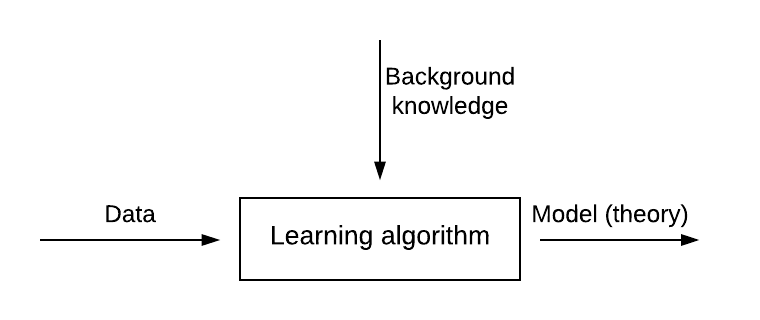
\includegraphics[width=0.7\columnwidth]{mlalgo}%
	\caption[The process of training a learning algorithm.]{\captionstyle{The process of training a learning algorithm. The algorithm analyses the data it receives as input, utilises previously generated knowledge (if it exists) and generates a model of the data. Adapted from \citep{Kononenko2007}.}}%
	\label{fig:mlalgo}%
\end{figure}


 The different types of ML algorithms are based on the type of training data they require. They can be classified as:
\begin{itemize}
	\item Supervised learning - the program is provided with manually labelled training data from which it gains knowledge. \enquote{Label} refers to the expected output for each object.
	\item Unsupervised learning - unlabelled data is provided so that the program discovers how objects are mapped to values without human assistance.
	\item Semi-supervised learning - both labelled and unlabelled training data are used. The algorithm learns how the labelled data is classified and classifies the unlabelled data in the same way.
	\item Reinforcement learning - the system is rewarded when it generates the correct output, and is punished when the output is incorrect.
\end{itemize}

What follows is a description of each method.

\subsubsection{Supervised Learning}
Supervised Learning requires training data which is labelled. By utilising an algorithm, the system tries to understand the mapping between each item in the dataset and its label. If it successfully does so, when given more unlabelled data, it should be able to predict what label each item corresponds to. This process resembles human learning with a teacher.

The disadvantages of this method are that the preparation of the training data requires manual annotation of each item by a human. For large data sets this could be a time-consuming task. Additionally, if the data is specialised in some area, a professional might be required for correct annotation.

There exists several supervised learning algorithms. They can be categorised based on their goal: \textit{classification} and \textit{regression}.

%\begin{figure}[htb]%
%	\centering
%	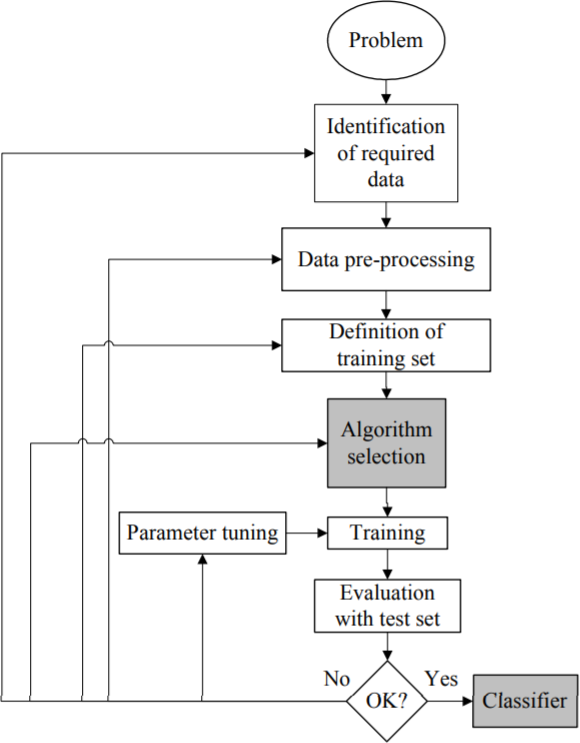
\includegraphics[width=0.5\columnwidth]{supervisedML}%
%	\caption{\captionstyle{The process of applying Supervised Machine Learning to a real-world problem \citep{Kotsiantis2007}.}}%
%	\label{fig:supervisedml}%
%\end{figure}

\myparagraph{Classification}
Classification is a method where a system is taught how to map an object to an attribute. To learn how to do this, it is provided with training data in which objects are mapped to their corresponding categories (classes) correctly. By utilising a classification algorithm, the system can analyse the data and discover the logic behind the mappings. After the training process, the system can categorise new objects based on its knowledge and assign a class to them from its set of known attributes. 

An example of classification would be using training data in the form of a list of RGB values of colours, where each value has the corresponding colour name assigned. After the system analyses them, it should be able to predict what colour new RGB values correspond to. 

Some classification algorithms are:
\begin{itemize}
	\item Na\"ive Bayes - based on probability. It assumes that the attributes of objects are independent within the context of the class \citep{mccallum1998comparison}. This is the most basic classification algorithm, however it has been known to produce satisfactory results.
	\item K-nearest neighbour - in this method, the training data is stored. When an object has to be classified, it is compared to the known objects with a distance function and the closest matches' class is assigned to the new object \citep{Kononenko2007}.
	\item Decision trees - the instances are sorted by their features in a tree-like data structure. The nodes of the tree correspond to attributes while the branches represent a possible value for the node. The objects are sorted by their attributes and the classification process starts from the root node \citep{Kotsiantis2007}.
\end{itemize}

\myparagraph{Regression}
In regression methods, the focus is prediction of numerical variables as opposed to the categories predicted in classification. These methods are usually used for the prediction of quantities, sizes, amounts, etc.

Some regression algorithms are:
\begin{itemize}
	\item Simple linear regression - these algorithms aim to predict one numerical variable based on a single attribute. For example, predicting the price of a smartphone based on its year of manufacture.
	\item Multiple regression - the goal is to predict one numerical variable based on multiple features. An example is predicting the price of a smartphone based on its RAM, processor and storage capacity.
	\item Logistic regression - 
\end{itemize}

\subsubsection{Unsupervised Learning}
Unsupervised learning methods do not use labelled data to gain knowledge. Instead, the goal is to discover how objects are related. The advantage of this method is that labelled data is difficult and time-consuming to produce and more unlabelled data exists.

In contrast to Supervised Learning, the aim is to find patterns within the data instead of prediction or classification \citep{Kononenko2007}. More uncertainty exists within unsupervised methods, however, since the results are limited to the provided data. If the data is incomplete, meaningless correlations might be found between items.

Unsupervised learning methods can be categorised as:
\begin{itemize}
	\item Clustering - aims to group the instances into coherent subsets \citep{Kononenko2007}. Items within one cluster display more similarity than items in other clusters. The task of the algorithm is to define the grouping criteria and cluster the objects accordingly. Clustering is often used in statistical analysis of data. The K-means algorithm is a popular choice.
	\item Association rule-mining - used for finding relationships between items. For example, online shops utilise this method to suggest products to users based on what they have bought previously. 
\end{itemize}

\subsubsection{Semi-supervised Learning}
Semi-supervised learning is useful in cases when a sufficient amount of labelled data is not present and it is difficult to acquire it. This method allows the usage of some annotated data and a larger amount of unlabelled data. Some possible techniques that can be used are:
\begin{itemize}
	\item Graph-based methods
	\item Generative methods
	\item Heuristic-based methods
\end{itemize}

\subsubsection{Reinforcement Learning}
Reinforcement Learning is method that utilises a trial-and-error technique to learn in an interactive environment. This method be implemented in 3-dimensional simulation, etc.

The agent in the system is programmed with instructions on how to interact with the world. Based on its surroundings, it performs an action. If the action contributes to the agent reaching the state it is aiming for, it is rewarded. On the other hand, if the action it performs is incorrect, it is penalised. Based on the result, the agent then changes its behaviour in order to receive a reward. This process is repeated until the agent has generated a set of rules (knowledge) needed to achieve its goal.

The main difference with unsupervised learning is the use case. In reinforcement learning, the agent aims to define a set of beneficial actions needed to reach a pre-specified task while in unsupervised learning the system attempts to find patterns within its input data.

\subsection{Natural Language Processing}
Natural language processing (NLP) is an area where multiple seemingly unrelated sciences are combined: AI, linguistics and Computer Science. \citet[17]{Goldberg2017} describe Natural Language Processing as a \enquote{collective term referring to automatic computational processing of human languages}. This definition applies for applications which receive natural language as input and programs which produce human-like text as output. In addition, \citet[17]{Goldberg2017} highlight that such functionality is needed as communication with a computer using natural language would be much simpler for humans. 

However, \enquote{understanding} language is a difficult task for machines, even though it is one of the first things humans learn. The problems occur due to the ambiguity of language and its constant evolution. Moreover, usually computers follow a set of instructions to perform a given task. However, language cannot be represented as a set of rules.

The initial approaches to NLP were simplistic and based on logical rules \parentext{e.g. ELIZA \citep{Weizenbaum:1966}}. Modern projects employ \textit{statistical methods} and \textit{neural networks} \citep{Goldberg2015}.

For an NLP system to successfully operate, it has to analyse and preprocess its input. \citet{Martinez2010} summarises the methods an NLP system might use to achieve this as:
\begin{itemize}
	\item Morphological – concerned with the structure of individual words.
	\item Syntactic – refers to the structure of each sentence and the rules of constructing them.
	\item Semantic – refers to the meaning of a piece of text.
\end{itemize}

\subsubsection{Morphological}
Morphemes are the smallest part of a word which conveys meaning. For example, when analysing the word “unhappily” morphologically, it can be divided into the following morphemes: \textit{-un} (prefix), \textit{happy} (root) and \textit{-ly} (suffix). Morphemes affect the meaning of words. For example, in the word “unhappily”, the prefix indicates that the opposite meaning of the root word is used, and the suffix shows that the word is an adverb. Another example would be words in the past tense which have the suffix \textit{-ed}. Since prefixes and suffixes do not change, it is relatively easy for an NLP system to process them.

\subsubsection{Syntactic}
Syntax is concerned with whole words as opposed to morphemes. The syntactic analysis aims to define the grammatical structure of a sentence.

NLP systems utilise different methods of analysing a text syntactically. Some common ones are presented below.

\myparagraph{Tokenisation}
Tokenisation is a process which converts a document to a set of tokens and removes certain characters \citep{Manning2008}. Usually punction, possessives and apostrophes in shortened words are stripped from the text. \citet{Manning2008} also makes the point that each language has different rules for punctuation and word joining which makes the process of tokenisation very language specific.

\myparagraph{Part of speech tagging}
This process aims to assign tags (labels) to each word based on the part of speech it represents. Possible approaches to this are Markov chains or Hidden Markov Models \citep{Martinez2010}. The former is useful when there is a large amount of already tagged data present, while the latter is preferable when training data does not exist \citep{Martinez2010}.

\myparagraph{Stop words removal}
Stop words are words that occur too often in a text and convey little meaning \citep{Martinez2010}. An approach to identifying them is proposed by \citet{Manning2008}: sorting all the terms by frequency of appearance and manually analysing the most common ones and storing the relevant entries (which convey no meaning) in a list of stop words. Every item in this list is then discarded when processing the text. A disadvantage of this method is the need for manual identification of the unnecessary phrases, although it could be more accurate than an automated one.

However, in some cases, stop words have an important role in a sentence, e.g. “Flight to London”. Removing the preposition “to” results in a loss of the meaning of the sentence \citep{Manning2008}. 

\begin{figure}[!htb]
	\begin{center}
	\begin{tabular}{@{}llllllllll@{}}
		\toprule
		a & an & and & are & as & at & be & by & for & from \\ 
		has & he & in & is & it & its & of & on & that & the \\
		to & was & were & will & with & & & & & \\ \bottomrule
	\end{tabular}
	\end{center}
	\caption{\captionstyle{Example list of stopwords. Adapted from \citep{Manning2008}.}}	
	\label{tbl:stopwords}
\end{figure}

\myparagraph{Stemming and lemmatisation}
Both stemming and lemmatisation aim to fix the problem with different forms of a word. For instance, the words “studying” and “studied” should both be interpreted as a derivation of the word “study”, rather than separate words \citep{Manning2008}.

\textit{Stemming} is the process of reducing a word to its root \citep{Martinez2010} by removing its suffixes, affixes and prefixes. An example would be converting the word “studied” to its root by removing the suffix for past tense \textit{-ed}. The result would be \textit{studi}. However, stemming the word \textit{studying} would produce \textit{study} which will not match \textit{studi}. The process, however, works well in some cases, e.g. \textit{going} would be converted to \textit{go} since the root does not change when the suffix “-ing” is added. Several stemming algorithms exist: Lovins stemming \citep{Lovins1968}, Paice stemming \citep{Paice1990}, and the most widely adopted algorithm in modern projects: Porter stemming \citep{Porter1997}.

\textit{Lemmatisation} aims to be more precise than stemming. In this case, the word \textit{studied} would be converted to the root \textit{study}. However, to successfully do this, the program would need a comprehensive dictionary with all possible forms of a word.

Both processes have advantages and disadvantages. Stemming is easier to implement as it follows direct rules, however, depending on the use case, the results might not be satisfactory. Lemmatisation, while producing more accurate results, would be more difficult to implement and would require accurate data. \cref{tbl:stemlem} illustrates the output of both processes when they are given the same input. 

\begin{table}[htb]
	\renewcommand\arraystretch{1.6}
	\caption{\captionstyle{Comparison of the results of stemming and lemmatisation of some words.}}
	\label{tbl:stemlem}
	\begin{tabularx}{\textwidth}{XXX}
		\toprule
		\textbf{Word} & \textbf{Stemming} & \textbf{Lemmatisation} \\ \midrule
		dogs          & dog                      & dog                           \\
		am, are, is   & am, ar, is               & be, be, be                    \\
		swam          & swam                     & swim                          \\ \bottomrule
	\end{tabularx}
\end{table}

Deciding which method to use would be based on the objectives of the software that is developed. For simpler cases, lemmatisation would perform well enough, however for more complicated use cases were accuracy is important, stemming would be the preferred aproach.

\subsubsection{Semantic}
Semantics refer to the meaning conveyed by a sentence \citep{Martinez2010}. As described in the previous sections, both morphology and syntax contribute to the meaning. A common problem that has to be solved in NLP systems is \textit{word-sense disambiguation}.

\myparagraph{Word sense disambiguation}
There exist words with multiple meanings. For instance, “right” could refer to a direction or it could mean that something is correct. Word-sense disambiguation aims to identify what meaning of such words was used in a sentence. \citet{Martinez2010} presents the following methods to achieve this:

\begin{itemize}
	\item Dictionary-based – lexical resources or thesauri are used. Generally, such methods 
	\item Supervised – training data with manually pre-labelled words is used (the meaning of each word is the label). Popular techniques are Bayesian classification and Information Theory. In terms of machine learning, this is a classification task.
	\item Unsupervised – clustering machine learning algorithms are used in this method. It is useful when no training data exists, or it is impossible to tag all the data. Some studies have shown it to perform at least as well as the supervised method \citep{Yarowsky1995}.
	-	Dependency parsing
\end{itemize}
	
Only a subset of the techniques described above might be implemented, depending on the goal of the application that is being developed.

\subsubsection{Approaches to NLP}
Different approaches to implementing NLP exist. The most used ones are described below.

\myparagraph{Rule-based}
Rule-based methods are based on the belief that natural language can be represented as a formal model. It is arguable whether this is true as language was not created, rather it came to be. Furthermore, natural languages have numerous variations, constantly change and are difficult to define. The meaning of each word or combination of words cannot be defined as a set of rules (referred to as \enquote{grammars}). As an example, the rules can be expanded to include all meanings of the verb \enquote{drink}. However, rules for the nouns \enquote{drink} can be used in conjunction with must be added as well since \enquote{drink} can be combined only with nouns which refer to liquids. Creating such rules for every word in a language manually would be tedious, error-prone, difficult to manage and inefficient. For this reason, better techniques were required.

Rule-based methods were the first approach to NLP that was invented. An early chatbot which utilised this method was ELIZA. As \citet{Weizenbaum:1966} explains, ELIZA analyses its input and matches each word with a dictionary of keywords. If there is a match, a pre-remade rule for this keyword is used to transform the sentence into appropriate output. 

While rule-based methods have been shown to work, they do not 
	
\myparagraph{Statistical}
Statistical approaches are based on calculating the probability of a string of words being a coherent sentence rather than comparing them to known words in a dictionary \citep{RusselStuart}. 
	
Methods used to achieve this are:
\begin{itemize}
	\item N – grams
	\item Naïve bayes
	\item Markov Chains
	\item Hidden Markov Models
\end{itemize}

%\myparagraph{N-gram character model}
%\[
%P(c_i|c_{1:i-1}) = P(c_i|c_{i-2:i-1})
%\]
%
%\[
%P(c_{1:N}) = \prod\limits_{i = 1}^{N} P(c_i | c_{1:i-1}) = \prod\limits_{i = 1}^{N} P(c_i | c_{i-2:i-1})	
%\]

\subsection{Summary}
This section introduced the roots of artificial intelligence with the ideas of Alan Turing and discussed the different branches of AI (Machine Learning and Natural Language Processing). The techniques which will most likely be used in the development of the application proposed in Section 1 will be a combination of Natural Language Processing and Machine Learning. 

Since the chatbot to be developed will have to answer specific fact-based questions, supervised learning methods will be used. Therefore, factual data will be required for the training process. Such data exist in abundance, both pre-compiled sets of technical data and online forums where such data is stored. 

\newpage
\section{Technology Review}
This chapter will describe what technologies were selected for the development of the chatbot.

\subsection{Chatbot Library}
The first choice made was what library or service to use for input processing. Libraries which are made specifically for chatbot development were investigated. Unfortunately, few options exist. The results of the investigation were the following frameworks: BotMan, Chatterbot and several online tools for chatbot creation.

\myparagraph{BotMan}
BotMan is a framework written in PHP. However, it uses a pattern-matching method for input processing. A question and an answer can be specified. Whenever the chatbot receives a question has in its rules, it returns the response to it. Even though BotMan could be considered a viable option, its main use case is the creation of marketing chatbots. However, the aim of this project is to implement chatbot which can answer a wide variety of questions on different topics. Additionally, the pattern-matching method would be insufficient for the purposes of this project. Lastly, BotMan is advertised a marketing chatbot creation tool and this is what it is most suitable for.

\myparagraph{Online tools for building chatbots}
Many such services exist, e.g. Microsoft Bot Framework, Wit.ai, Dialogflow, IBM Watson, Pandorabots, Botpress. However, their use case is similar to BotMan's - the creation of marketing chatbots. Furthermore, such services are very limiting as their creation does not involve any programming. Lastly, these services are paid. While some do offer free plans, they provide extremely limited resources and limit the traffic to the application.

\myparagraph{Chatterbot}
Chatterbot is a Python library for creating general purpose chatbots. It utilises Machine Learning and NLP to match the user input to a database of known data in order to find the most similar statement. It is open source and extendible and has comprehensive documentation. 

In conclusion, the Chatterbot library is the most suitable choice for the development of this project as it is extensible, utilises NLP to compare user input to known data and is highly configurable.

\subsection{Chatterbot}
The main technology used for the development of the project will be the python module \textit{Chatterbot}. It provides a simple way to generate a response to user input \citep{Chatterbot:online}. It was specifically created in order to help programmers develop chatbots.

\subsubsection{Overview of Input Processing}
\cref{fig:chatterbot-process-flow} illustrates how Chatterbot works on a high level. Firstly, the user inputs a statement (their question). It is then processed by the \textit{logic adapters} of the chatbot and the response with the highest value of confidence is returned to the user.

\begin{figure}[!htb]%
    \centering
    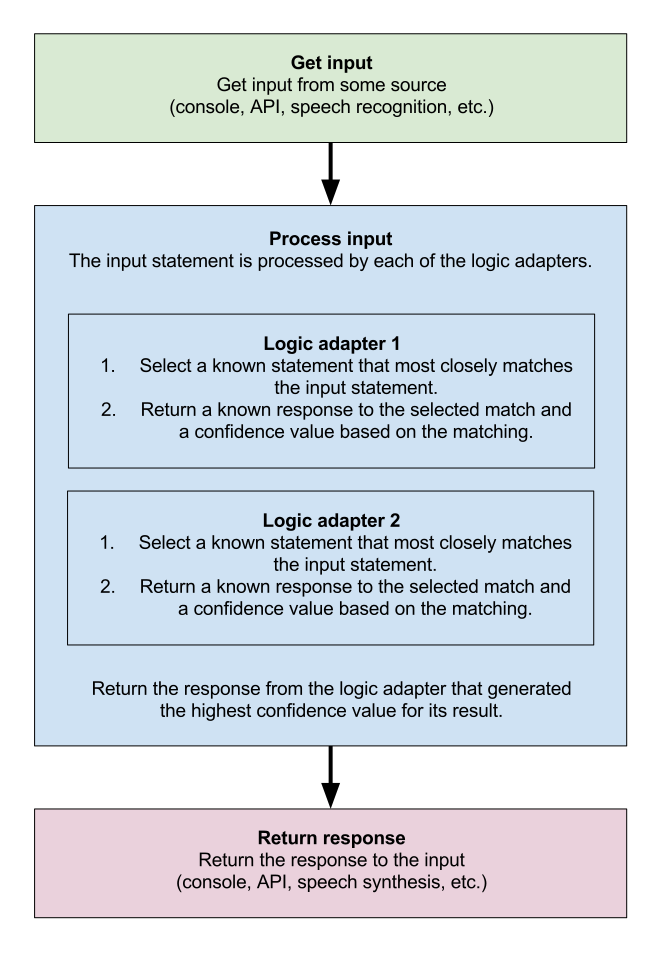
\includegraphics[width=0.6\columnwidth]{chatterbot-process-flow}%
    \caption{\captionstyle{Diagram of the process of receiving input, processing it and generating a response \citep{Chatterbot:online}.}}%
    \label{fig:chatterbot-process-flow}%
\end{figure}

\subsubsection{Configuration}
Chatterbot provides a \texttt{ChatBot} class. An instance of it takes several parameters in its constructor which define its behaviour:
\begin{itemize}
    \item \texttt{preprocessors}
    \item \texttt{logic\_adapters}
    \item \texttt{storage\_adapters}
\end{itemize}

\subsubsection{Preprocessors}
The \texttt{ChatBot} instance can take a list of functions in its constructor to be used as preprocessors. Preprocessors can modify the input sent by the user before it is passed to the logic adapters. This is necessary due to the fact that the logic adapters are more likely to perform better if they receive clean input. For example, if the input contains a lot of white spaces or non-alphanumerical characters, it might be beneficial to remove them. Chatterbot has several preprocessors built in, however, custom functions can be created and used as preprocessors.

\subsubsection{Logic Adapters}
\textit{Logic adapters} are used to select an appropriate response to a question entered by the user. More than one logic adapter may be used as different types of input may require different processing. For example, Chatterbot by default uses the \texttt{BestMatch} logic adapter. However, it is only useful when the question asked has a specific response. If the user asked for the current time, the \texttt{BestMatch} adapter would be unable to answer as there is no specific answer to this question, i.e. the answer changes depending on when the user asks the question. For this reason, a \texttt{Time} logic adapter can be created and added to the list of adapters used (Chatterbot has this adapter implemented by default). 

To help decide which adapter to use if more than one are provided, a custom logic adapter must inherit from the base class \texttt{LogicAdapter} and must implement the method \texttt{can\_process()}. This method is called before the logic adapters generate a response and the user input is passed to it. It must then return \texttt{True} or \texttt{False} based on whether the adapter can process this question. \cref{lst:canprocess} shows a possible implementation of the \texttt{can\_process} method. This example tells the adapter to only process user input which contains the string \enquote{Hey John} (John could be the name of the chatbot) in its beginning.

\begin{lstlisting}[caption={\captionstyle{Example implementation of the \texttt{can\_process()} method. Adapted from \citep{Chatterbot:online}.}}, label={lst:canprocess}]
    def can_process(self, statement):
        # If the statements starts with
        # the string 'Hey John',
        if statement.text.startswith('Hey John')
            # it can be processed with this adapter
            return True
        # If not,
        else:
            # it can't
            return False
\end{lstlisting}

Another requirement is that custom logic adapters implement the \texttt{process()} method. It takes the input statement as a parameter. Additional response selection parameters can be added if required by the application. 
%An example implementation can be seen in \cref{lst:process}.
%
%\begin{lstlisting}[caption={\captionstyle{Example implementation of the \texttt{process()} method. Adapted from \citep{Chatterbot:online}}}, label={lst:process}]
%    def process(self, input_statement, additional_response_selection_parameters):
%        import random
%
%        # Randomly select a confidence
%        # value between 0 and 1
%        confidence = random.uniform(0, 1)
%
%        # For this example,
%        # the input will just be returned
%        # as output
%        selected_statement = input_statement
%        selected_statement.confidence = confidence
%
%        return selected_statement
%\end{lstlisting}
This method must return a \texttt{Statement} object. The \texttt{text} property of the object should contain the actual response to the input, while the \texttt{confidence} property should be a value between 0 and 1 which indicates how confident the adapter is that this response is correct. 

%In the example above, the text of the output statement is set to the same text that was entered by the user. The confidence value is chosen randomly and the response is returned.

In the event that more than one logic adapters are used, and more than one of them returns a response, the response with the highest value of confidence is selected. If two or more responses have the same value of confidence, then the response of the adapter which is first in the list of adapters is used. \cref{fig:dialog-processing-flow} show a diagram of response selection with multiple adapters.

\begin{figure}[!hb]%
    \centering
    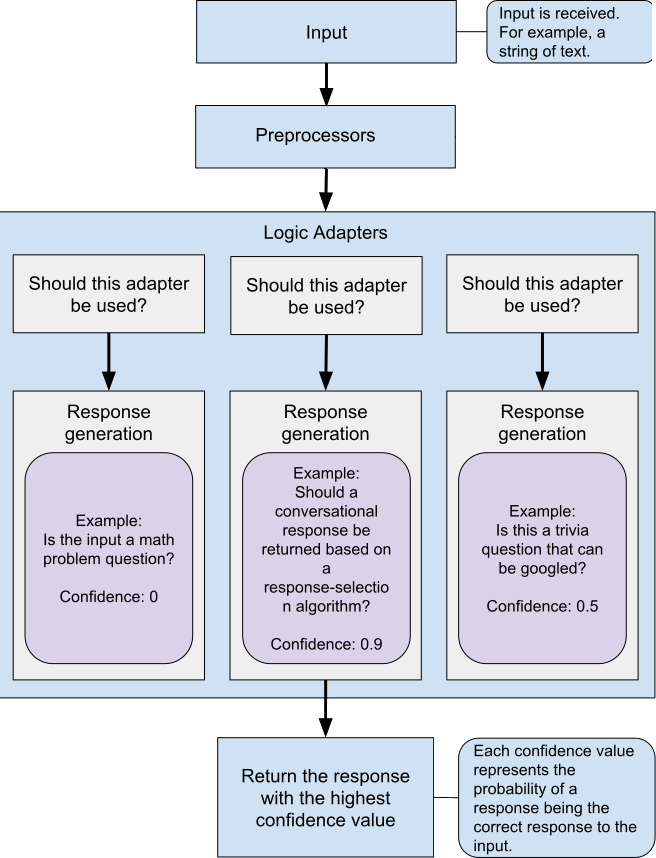
\includegraphics[width=0.9\columnwidth]{dialog-processing-flow}%
    \caption[Process flow diagram of how responses are selected]{\captionstyle{Process flow diagram of how responses are selected. In this example, the final response is the one generated by the adapter in the middle as its confidence is 0.9 which is greater than the responses from the other 2 adapters. Adapted from \citep{Chatterbot:online}.}}%
    \label{fig:dialog-processing-flow}%
\end{figure}


By default, Chatterbot has the following adapters included:
\begin{itemize}
    \item Best Match Adapter - used when question that have a specific response are asked. It requires training data and the quality of the response depends on the quality of the training data. The adapter uses a specific \textit{similarity} function to search through the known questions. When it finds the most similar one, it then returns the known response to this question. The similarity functions available by default are:
        \begin{itemize}
            \item Levenshtein Distance - this method is used by default. It calculates how many characters need to be changes 
            for one string to become the same as another. It is used to compare 2 strings an it returns a value showing how similar they are.
            \item Jaccard Similarity
            \item Sentiment Comparison
            \item Synset Distance
            \item Custom similarity functions may be implemented if needed.
        \end{itemize}
    \item Time Logic Adapter - allows the user to ask about the current time.
    \item Mathematical Evaluation Adapter - calculates mathematical expression the user has entered.
    \item Specific Response Adapter - returns a specific predefined answer to a specific statement configured in the adapter.
\end{itemize}

\subsubsection{Storage Adapters}
\textit{Storage Adapters} allow a ChatBot to use different storage technologies such as a database. The storage adapter used by default is the \texttt{SQLStorageAdapter}. It allows the chatbot to store its data in a local \texttt{SQLite} relational database. The structure of the database can be seen in \cref{fig:db-schema}. It consists of 3 tables:

\begin{itemize}
	\item \textbf{Statement} - stores the processed training data. The field \texttt{text} contains each response as it is seen in the training data. \texttt{search\_text} stores the processed response text, i.e. stop words are removed, a basic form of word-sense disambugation is applied where each word is replaced by its root or a synonym and each word is labelled with its corresponding part of speech. \texttt{in\_response\_to} contains the question that each response was assigned to in the training data. Lastly, \texttt{search\_in\_response\_to} contains the processed version of each question from the training data.
	\item \textbf{Tag} - each unique category found in the training data is added to this table.
	\item \textbf{Tag association} - shows what category each statement is assigned to.
\end{itemize}

\begin{figure}[!htb]%
    \centering
    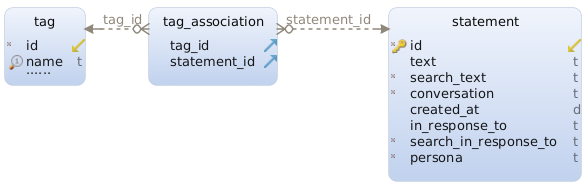
\includegraphics[width=0.9\columnwidth]{db-schema}%
    \caption{\captionstyle{The table structure of the relational database used to store the \enquote{knowledge} of a chatbot.}}%
    \label{fig:db-schema}%
\end{figure}


\subsubsection{Training}
%Chatterbot includes tools that help simplify the process of training a chatbot instance. ChatterBot’s training process involves loading example dialogue into the chatbot’s database. This either creates or builds upon the graph data structure that represents the sets of known statements and responses. When a chat bot trainer is provided with a data set, it creates the necessary entries in the chatbot’s knowledge graph so that the statement inputs and responses are correctly represented. An example of this can be seen in \cref{fig:training-graph}.

Training a ChatBot instance is achieved with the help of training data which represents conversations. The data is analysed, processed and each statement and it's corresponding answer are added to the database of the chatbot. The processing involves removing stop words, removing punctuation, tagging each word with its corresponding part of speech and replacement of some words with synonyms.

%\begin{figure}[!htb]%
%    \centering
%    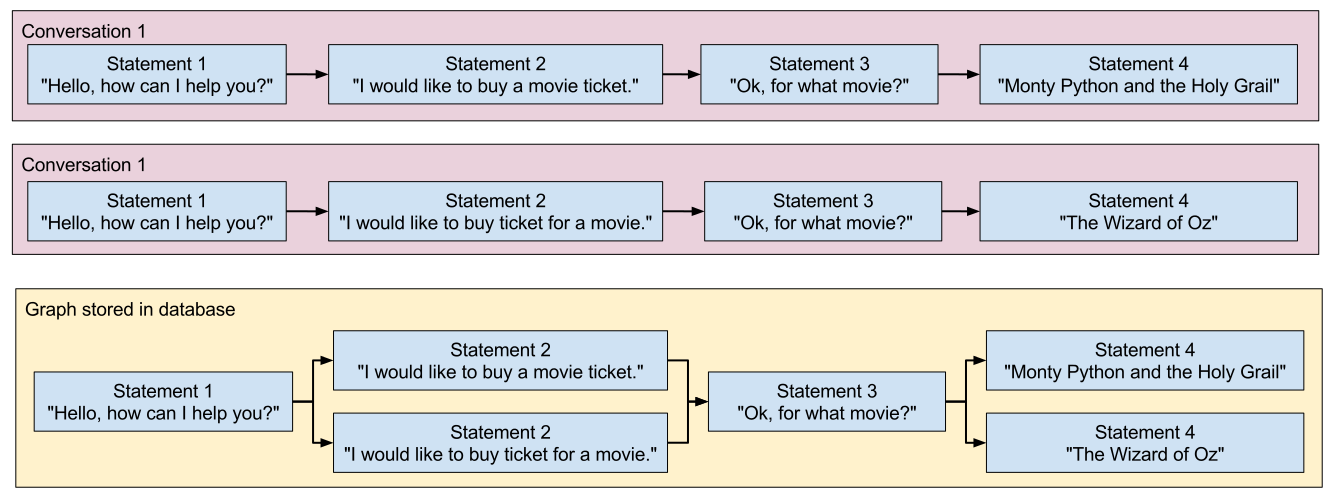
\includegraphics[width=1.0\columnwidth]{training-graph}%
%    \caption{\captionstyle{Example of a training graph \citep{Chatterbot:online}.}}%
%    \label{fig:training-graph}%
%\end{figure}

Chatterbot includes the following trainers:
\begin{itemize}
    \item List Trainer - trains the chatbot with data stored in a list.
    \item Corpus Trainer - trains the chatbot with data stored in an external file.
\end{itemize}

Custom trainers can be implemented. They must extend the class \textit{Trainer} and implement the method \texttt{train()}.

%\subsubsection{Statements}
%Chatterbot’s statement objects represent either an input statement that the chat bot has received from a user, or an output statement that the chat bot has returned based on some input.
%
%Chatterbot stores knowledge of conversations as statements. Each statement can have any number of possible responses.
%
%\begin{figure}[!htb]%
%    \centering
%    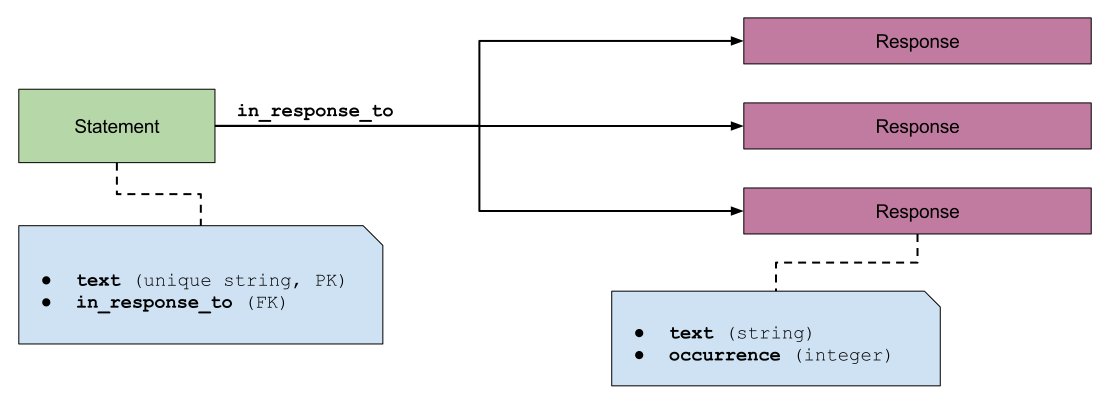
\includegraphics[width=1.0\columnwidth]{statement-response-relationship}%
%    \caption{\captionstyle{Statement-response relationship \citep{Chatterbot:online}.}}%
%    \label{fig:statement-response-relationship}%
%\end{figure}
%
%Each Statement object has an \texttt{in\_response\_to} reference which links the statement to a number of other statements that it has been learned to be in response to. The in\_response\_to attribute is essentially a reference to all parent statements of the current statement.

%\begin{figure}[!htb]%
%    \centering
%    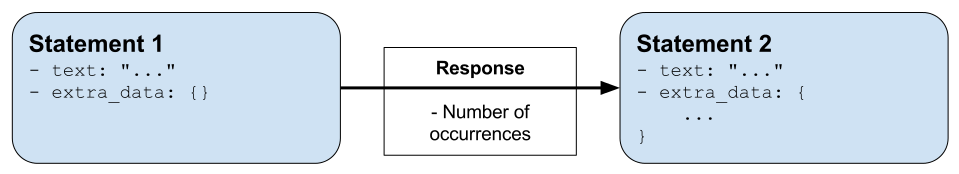
\includegraphics[width=1.0\columnwidth]{statement-relationship}%
%    \caption{\captionstyle{Statement relationship \citep{Chatterbot:online}.}}%
%    \label{fig:statement-relationship}%
%\end{figure}

%The count of recorded statements with matching, or similar text indicates the number of times that the statement has been given as a response. This makes it possible for the chat bot to determine if a particular response is more commonly used than another.

\subsubsection{Generating a response}
After the ChatBot instance has been initialised and trained, a response can be generated by calling the method \texttt{get\_bot\_response()}. It takes a string containing a question as a parameter and returns the response of the chatbot.

The response generation is achieved by preprocessing the question with the same NLP techniques used when training data is learned. A response can then be retrieved from the database by using a SQL \texttt{SELECT} statement which finds a statement with a value for \texttt{in\_response\_to} which matches the processed input.

\subsection{Python}
Since the main library used for the development of the project is written in Python, the decision to implement the application in the language was made. 

Python is known to greatly reduce development time as it provides a lot of \enquote{syntactic sugar}. Another advantage is its automatic garbage collection. In traditional programming languages such as \texttt{C++} manual memory management is an issue for new programmers and security and performance issues might occur when it is not implemented correctly. 

Python is a weakly-typed language, which means that variable types are deduced by the python interpreter. For this reason, developers do not have to specify the type of variable they are declaring. However, this could lead to problems as the type of data stored in each variable has to be remembered since assigning a different type later would result in an error. Moreover, Python is a high-level language, meaning that it provides more layers of abstraction. This results in the writing of less code to solve a specific problem.

Python has a large selection of modules. Additionally, Python is a multi paradigm language, i.e. it supports object-oriented programming, functional programming, imperative programming and procedural programming. Lastly, it is a cross platform language, being able to run on most major operating systems.

Similarly to other programming languages, Python does have disadvantages. The main one is that it is an \textit{interpreted} language. This means that rather than compiling the code to an executable file (machine code), the python interpreter reads it line by line and executes each instructions. Another problem caused by this is that errors can only be found during the runtime of a program. If a function of the software is rarely executed, issues with it might not be discovered. This issue can be solved relatively easily. For example, unit tests can be written which execute all functions of a program. Even though this problem doesn't exist with languages such as C++, where errors are reported during compilation, programs still have to be tested for logical errors.

\subsection{Flask}
Another important decision that had to be made was what type of application to develop. The options considered were: a smartphone app, a program which targets desktop operating systems (Windows, Linux or Mac) or a web app. Since the main goal was to make the deliverable accessible from any platform, the idea of smartphone app was disregarded. Furthermore, the main mobile platforms have very different development tools and processes. A desktop application was not implemented for the same reasons - it would only work on one type of device and targeting all desktop OSs would be a difficult task. In contrast, a website, would be accessible from any device which can be connected to the Internet and has a browser program. Incidentally, all the devices mentioned above, mobile devices and PCs, have this functionality.

The technologies considered initially were PHP for the development of the website and MySQL for database interaction. However, since the goal was to implemented a simplistic website, it was decided that the difficulty of setting up a PHP server would outweigh the benefits. It was also unclear how the communication between the Python library and a PHP program would be implemented. Instead, methods for web development in Python were investigated. The results showed that Python has become a popular choice for website creation with its 2 popular frameworks Flask and Django. Ultimately, the decision to use Flask was made as it provided a smaller subset of tools which was enough for the creation of a simplistic web app. Furthermore, Flask was easier to set up and configure.  

Flask is a micro framework for Python used for website development \citep{Flask:online}. It is described as a microframework as it aims to only include the core functionality required to create a website. For instance, by default, Flask does not include any database interaction functionality. However, it would not be required since it is implemented by Chatterbot.

Flask includes a server which can be used for development, page routing and templating. 

The page routing functionality allows Flask to create multiple pages within one website and users to access them.

The templating engine extends the functionality of HTML. Templates are HTML files which can include special tags which are processed by the Flask server. One common usage is passing variables from a Python script to the HTML code so that its value can be displayed. When the user accesses a page, its template is converted to static HTML by the template engine (Jinja) and it is displayed to the user. Templates also allow the reusability of code since one template can extend another, i.e. the contents of the former can be automatically appended to the templates of the latter.
 
\subsubsection{Twitter Bootstrap}
Since the goal was to implement a website which could be used from any device which can access websites, Twitter Bootstrap was used. It is a CSS framework which provides a responive design functionality. It allows the positioning elements in a grid of rows and columns. When the page is resized, the columns are re-ordered and their size is changed dynamically to fit the page. The font size is also modified based on the resolution of the device.

\subsection{Pytest}
As explained above, one of the disadvantages of Python is that errors might not be discovered until the code is thoroughly tested. However, often it is not possible to test all aspects of a program manually after making changes to the code. For this reason, an automated testing system was planned. Unit tests were a method to achive this. The Python library Pytest was selected as the unit test framework since it is recommended by the Flask documentation \citep{Flask:online} and it is supported by Flask.


\subsection{Web Hosting}
Since the project implements a website, web hosting options were considered so that the website can be made public. Traditional web hosting options could not be used as they offer PHP servers with MySQL databases. Instead, web hosting services which support Python and Flask were considered. The main options were:
\begin{itemize}
	\item Amazon AWS 
	\item Heroku
	\item Python Anywhere
\end{itemize}

All these services are viable options, however both AWS and Heroku have a limit of requests for their free tier. If the limit is exceeded, payment is taken from the website owner’s account. Python Anywhere, on the other hand, is free. Furthermore, it is the easiest to set up as it supports Flask websites by default.

\newpage
\section{Implementation}\label{sec:impl}
During the Interim Meeting in week 9 of semester 1, the second marker of this project proposed that deliverable could have a specific purpose to simplify the evaluation process. Evidence of this is provided in \cref{app:interim} (see "Any other recommendations as to the future of the project?").  The advice was taken and the objectives of the project were changed. The initial idea can be seen in \cref{app:ipo}. \fullref{subsec:aims} introduces the new project aims. Therefore, this section will discuss the implementation process of the new project.

\subsection{DevOps}
This section explains the development operation methodologies used during the implementation process.

\subsubsection{Management}
An Agile workflow was adopted. Each week was considered a sprint and a working build of the application was deployed at the end so that it can be demonstrated during the meetings with the supervisor of the project. A prioritised sprint backlog was created for each sprint with the application Trello. An example backlog can be seen in \cref{fig:backlog}.

\begin{figure}[!htb]%
	\centering
	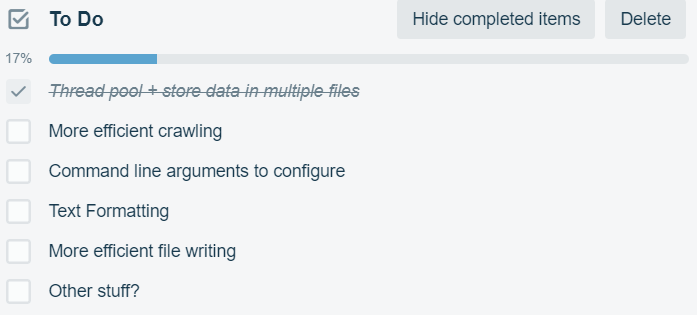
\includegraphics[width=1.0\columnwidth]{backlog}%
	\caption[An example of a prioritsed sprint backlog.]{\captionstyle{An example of a prioritised sprint backlog. The items on top have a higher priority and should therefore be implemented first.}}%
	\label{fig:backlog}%
\end{figure}

Additionally, a project plan was created in the form of a Gantt Chart (\cref{app:gantt}). Goals were set for each iteration and milestones were defined. 

\subsubsection{Version control}
Version Control was used in the development of the project. The version control system used was \textit{Git} and the repository was hosted on \textit{GitHub}. The reason for this was previous experience with these technologies. 

Using Git and Github meant that the source code of the application could be easily shared between computers. Additionally, changes between versions of the program could be tracked. In the event that issues arose, the application could be reverted to a previous working version. If necessary, the difference in the source code between two versions could be inspected.

Another feature of Git and Github used was \textit{branches}. Branches allow for having several versions of the code at the same time. The following branches were created for this project:
\begin{itemize}
	\item Master branch - a stable version of the application. It is thoroughly tested and no known bugs are present. The purpose of this branch is to contain the version of the code which can be deployed.
	\item Development branch - the most recent updates to the application which might not be fit for deployment. It can be updated until it is considered stable enough. It can then be merged into the master branch and deployed.
	\item Feature branches - a branch where a specific feature is implemented without affecting any of the other versions. It can be used for testing ideas or implementing a major new feature.
\end{itemize}

Using branching proved to be beneficial as the project was made publicly available early in the development process. Since continuous deployment was implemented, having a single branch was insufficient as unstable changes would cause problems in the live version of the website.

\subsubsection{Testing}
Since the application consisted of many components communicating with each other, problems were often encountered during the development process. For example, the chatbot expects to find the training data in a specific location. Therefore, the web crawler has to store the data in this exact location. To ensure changes would not break the current functionality, unit tests were implemented with the Python library PyTest. 

The first set of unit tests written was for testing the command line interface. Many modifications and updates were made to the web crawler during the development process. This always resulted in problems with the command line interface functionality as most of the commands modify the output of the crawler.

The second set of tests was for the chatbot functionality. These tests use PyTest fixtures which set up the necessary conditions before the tests are executed and delete any files or data left after they are run. These tests ensure the output produced by the chatbot is correct. 

The last set of unit tests implemented was for the storage adapter. Its ability to interact with the database is tested. 

\subsubsection{Code Coverage}
The PyTest library supports extensions. One such extension is pytest-cov which generates code coverage reports. Code coverage is a metric used to specify how many lines of code are executed when unit tests are run. For example, a code coverage of 100\% means that all of the code in the project is tested. Therefore, the higher the code coverage, the better. 

The pytest-cov coverage reports show detailed information about each file in the program that is tested. The code coverage for each file is shown as well as how many lines of code were not tested. At the end of the report, the average code coverage is shown. An example report can be seen in \cref{lst:codecov}.

\begin{lstlisting}[caption={\captionstyle{A code coverage report produced with pytest-cov.}}, label={lst:codecov},numbers=none]
Name                   Stmts   Miss  Cover
------------------------------------------
chatbot/__init__.py       49     24    51%
chatbot/bot.py            86      9    90%
chatbot/config.py          3      0   100%
chatbot/constants.py      22      0   100%
chatbot/crawler.py        80      6    92%
chatbot/logic.py          69     13    81%
chatbot/models.py         29      1    97%
chatbot/run_it.py          2      0   100%
chatbot/storage.py       199     51    74%
------------------------------------------
TOTAL                    539    104    81%    
\end{lstlisting}

The aim for this project was to achieve a code coverage of at least 85\% which was accomplished. Since a lot of libraries were used, it was impossible and infeasible to test all the code in the project. It was assumed the creators of libraries have tested their code thoroughly. Moreover, most libraries provide their own unit tests.

\subsubsection{Continuous Integration \& Deployment}
A Continuous Integration service could be used to automatically execute the unit tests every time new code is added to the GitHub repository. Changes were made to the project daily, however running the tests after each change was time-consuming. Using Continuous Integration meant that every time a commit was pushed to the GitHub repository, the tests would be run automatically, and any issues would be found quickly. Furthermore, since branches were used, the tests could be run after merging changes into the master branch. This allowed for the discovery of integration problems.

The Continuous Integration service used was Travis CI due to previous experience. It is used for continuous testing and delivery of projects hosted on GitHub. To set it up, the GitHub account which contains the project repository was linked to Travis CI. 

Configuration of the build process is achieved by adding a “.travis.yml” configuration file in the root directory of the repository. The file is written in the YAML format. Firstly, the operating system used to compile the project is specified. In this case \texttt{Ubuntu 16.04 (Xenial Xerus)} OS is used. Additionally, the language of the program was developed in is specified, i.e. Python. The versions of the language can be specified next. In this case, the project is tested with Python 3.6 and 3.7 which are the latest versions at the time of writing. Travis CI also supports the following steps:
\begin{itemize}
	\item \texttt{install} – this step is executed before the testing happens. It is used to install any packages that are not installed on Ubuntu by default. In this case, there are no packages that should be installed, however the libraries used in the project are downloaded via the package manager \texttt{pip} package manager.
	\item \texttt{before\_script} – this step occurs before the test script is executed. It is used to set the environment variables Flask expects. 
	\item \texttt{script} – this step executes the command which runs the unit tests. In this case, it is the \texttt{pytest} command. No other setup is required as pytest is able to discover unit tests without any additional configuration. However, since code coverage reports can be generated, the optional parameter \texttt{--cov} is added so that a coverage report is created.
	\item \texttt{after\_success} – this step is only executed after the tests have completed without any errors. The coverage report generated in the previous step is uploaded to codecov.io. It can then be inspected in detail. Codecov.io provides in-depth reports and charts of code coverage. Each file in the repository can be seen and it is shown whether each line is tested. This is useful for finding possible problematic areas which are not tested. 
	\item \texttt{cache} – this option specifies dependencies or folders which do not change often. They can be cached, instead of being downloaded every time the build process is run. In this case, the \texttt{pip} dependencies can be cached which speeds up the testing process.
\end{itemize}

\myparagraph{Continuous Deployment}
Since the website was hosted on Python Anywhere, Continuous Deployment could be implemented. This was done for faster deployment every time code was added to the master branch. This had to be implemented manually since neither Python Anywhere nor Travis CI had any methods of deploying Flask websites. 

The first step was to create an end point in the website. It was created at “/webhook”. It’s purpose was to receive requests from GitHub. Additionally, GitHub's webhook feature was configured to send a request to the live website’s “/webhook” address whenever a commit was added to the master branch. 

The website is configured to inspect the request body when it receives a request. It is checked whether the event that occurred is a commit and whether the commit was made to the master branch. If this is the case, changes from the repository can be pulled directly. This was achieved with the Python library GitPython. Unfortunately, when changes are made to the website, Python Anywhere requires the site owner to reload the website. This has to be done manually by going to the site settings and pressing a \enquote{reload} button. Python Anywhere has an API which provides an end point for reloading a website remotely, however, this cannot be done from the same program that runs the server as the request times out due to the server going offline for reloading. 


\subsection{Application}
One of the main early considerations was how to structure the source code. It became clear that the application should consist of two main parts: a back-end and a front-end program. Since the user will interact with a user interface (the front-end) and another program will process their input, it was logical to separate the two.

\subsection{Back-end}
The back-end program consists of a web crawler and a response generation program. The former is used to collect training data from Stack Overflow, while the latter processes the user input and generate a suitable response.

\subsubsection{Web Crawler}\label{subsub:crawler}
Before creating the back-end program, it was necessary to collect training data for the chatbot. The possible sources of data were online resources and books. 

There exist numerous books about programming languages and techniques. However, it was decided that this approach was infeasible as the Chatterbot library required training data in the format \textit{question - answer}. Extracring data from a book into this format would require advanced knowledge of NLP and the development of another program for this specific task.

Another option for data collection was websites which provide beginner tutorials about programming. However, limited amount of information of questionable quality was mainly available.

Ultimately, the decision to scrape \footnotemark[1] the website Stack Overflow was made. Stack Overflow is one of the most popular websites where programmers can ask questions about any programming language. Furthermore, there is a voting system which sorts the answers by number of votes. Additionally, the person who asks a question is able to mark a specific answer as the \enquote{accepted answer}. This meant that when collecting data, the answers to each question could be sorted by number of votes, and the \enquote{accepted answer} could be used as the default response of the chatbot. Unfortunately, some questions have no accepted answer or no answers at all.
 
\fancyfootnotetext{1}{Web scraping - a technique for extracting information from a website.}

It was decided that data about the \texttt{C++} programming language would be collected for the prototype of the application. It is a language often used at universities to introduce students to advanced concepts of computing. However, new programmers often find it difficult to understand concepts such as pointers, references, memory management. 

For the data collection process, a program was written with the Python module \textit{BeautifulSoup}. It needs the following parameters to operate:
\begin{itemize}
    \item \texttt{start\_page} - the first page to be crawled.
    \item \texttt{num\_pages} - total number of pages to be crawled.
\end{itemize}

With these values, additional required parameters can be calculated: the last page to be crawled is the sum of \texttt{start\_page} and \texttt{num\_pages} and current page (indicating which page is currently processed) is initially set to the value of \texttt{start\_page}. With this data, a loop can be executed, starting from the first page and running until the last page. In each loop iteration, a URL is generated to the corresponding Stack Overflow page. The structure of a Stack Overflow URL can be seen in \cref{fig:so-url}. The output of the page can be modified by changing the values of the highlighted parameters:
\begin{itemize}
	\item \textbf{base URL} is a constant value.
	\item \textbf{tag} is used to filter questions based on their category. In this case, \texttt{C++} questions are requested as \enquote{\texttt{\%2b}} expands to the symbol \enquote{\texttt{+}}. However, the tag can be changed to any language. For instance, to collect data about Java, the tag parameter can be given the value \enquote{java}.
	\item \textbf{sort} configures the order in which the questions are shown. In this case sorting by \texttt{votes} results in the most upvoted questions being shown first.
	\item \textbf{page} indicates the currently displayed page of results. Since there are numerous questions on the website, it is impossible to display them in one page.
	\item \textbf{pagesize} indicates how many questions are shown per page.
\end{itemize}

To generate a URL, all the parameters are appended to the base URL, and the \textbf{page} parameter is dynamically generated based on the \texttt{current\_page} variable.

%Another variable, \texttt{current\_page} (indicating the currently scraped page), is initially set to the value of the starting page variable. Then a \texttt{while} loop is executed until the value of \texttt{current\_page} becomes the same as the value of start + num\_pages, where \texttt{start} is the starting page and \texttt{num\_pages} is the number of pages to be crawled. The value of \texttt{current\_page} is incremented by one at the end of each loop iteration. In the beginning of each loop iteration, a URL of the page to be scraped is generated. This is achieved by appending several \textit{GET} parameters to the base Stack Overflow URL. The structure of a Stack Overflow URL can be seen in \cref{fig:so-url}.
%The \textbf{base URL} is a constant value. The \textbf{tag}, \texttt{c\%2b\%2b} in this example, is used to show only questions categorised as relate to the programming language. In this case, \texttt{C++} questions are requested as \texttt{\%2b} expands to the symbol \texttt{+}. However, the tag can be changed to any language or technology. For instance, to collect data about Java, the tag can be changed to \texttt{java} and this would result in only extracting data from Java-related questions. The \textbf{sort} parameter indicates the order in which the questions are shown. In this case sorting by \texttt{votes} results in the most upvoted questions being shown first. The \textbf{page} parameter indicates the current page. Since there is a large number of questions on the website, it is impossible to display them in one page. The last parameter used is \textbf{pagesize}. It indicates how many questions should be shown per page. To generate a URL, all the parameters are appended to the base URL, and the \textbf{page} parameter is dynamically generated based on the \texttt{current\_page} variable. 

\begin{figure}[!htb]%
    \centering
    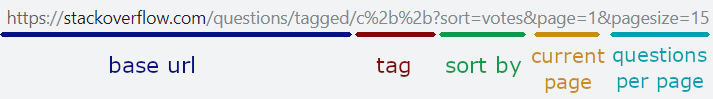
\includegraphics[width=1.0\columnwidth]{so-url}%
    \caption[The structure of a Stack Overflow URL.]{\captionstyle{The structure of a Stack Overflow URL. Variables and their values are appended to the base url. The separator used is \texttt{\&}.}}%
    \label{fig:so-url}%
\end{figure}

With the generated URL, the page can be accessed from within a Python program with the library \textit{requests}. The returned result is the source code of the page at the given URL. Data can then be extracted from it using the \textit{Beautiful Soup} Python library. Firstly, an instance of the \texttt{BeautifulSoup} class is created. The source code retrieved earlier is passed to it. The library can then parse it and create a \textit{parse tree} which as an efficient data structure for storing hierarchical data. 

The data needed from each page of questions is the hyperlink to each question. To extract this data, the method \texttt{find\_all()} of the \texttt{BeautifulSoup} object can be used. It returns a list of all the occurrences of a specified HTML tag. In this case, the HTML \texttt{<a>} tag is needed as it is used to create hyperlinks. However, there are numerous hyperlinks on each Stack Overflow page. Only the hyperlinks which lead to a question page are needed. Using the Chrome browser developer tools, it was discovered that each link to a question was assigned a class value \enquote{question-hyperlink}. \cref{lst:hyperlink} shows the HTML code of an example hyperlink to a question.

\begin{lstlisting}[language=html, caption={\captionstyle{An example hyperlink to a Stack Overflow question.}}, label={lst:hyperlink}]
    <a href="/questions/121162/what-does-the-explicit-keyword-mean" class="question-hyperlink">What does the explicit keyword mean?</a>
\end{lstlisting}

With this information, only the URLs of the questions could be extracted. \cref{lst:extract-questions} shows the source code for extracting the hyperlinks to each question. The \texttt{find\_all()} method on line 3 returns a list of all \texttt{<a>} tags with a class value "question-hyperlink". A for-each loop iterates through this list. Each hyperlink's destination is extracted from the \texttt{href} parameter using the \texttt{get()} method. Each link's text is also extracted using the \texttt{get\_text()} method. The destination URL, however, is incomplete and it needs to be appended to the base Stack Overflow URL. The final question URL and the question title are passed to the \texttt{parse\_question()} method. The if statement on line 4 is needed as there is a "Hot Network Questions" section on each Stack Overflow page which contains hyperlinks to popular questions. The if statement ensures these links are not processed.

The \texttt{parse\_question()} method can be seen in \cref{lst:extract-answers}.

\begin{minipage}{\columnwidth}
	\begin{lstlisting}[caption={\captionstyle{Extracting answers for a specific Stack Overflow question.}}, label={lst:extract-answers}]
	def parse_question(url, title, data):
	# page to be scraped
	page = requests.get(url, headers=headers, timeout=(3, 30))
	# initialise bs4
	soup = BeautifulSoup(page.content, 'lxml')
	# get the question data, contained in a <div> with class "postcell"
	question = soup.find('div', class_='postcell')
	if question is not None:
	answers = soup.find_all('div', class_='answercell')
	# limit to max 3 answers per question
	end = len(answers)
	if end > CRAWLER_NUM_ANSWERS:
	end = CRAWLER_NUM_ANSWERS
	# for each answer found
	for i in range(0, end):
	# get the answer text
	answer = answers[i].find('div', class_='post-text').extract()
	# store the question and the answer in their own list
	answer = str(answer)
	entry = [title, answer]
	# add to the main list
	data.append(entry)
	\end{lstlisting}
\end{minipage}

\begin{minipage}{\linewidth}
	\begin{lstlisting}[caption={\captionstyle{Extracting the URL of each question on a Stack Overflow page.}}, label={lst:extract-questions}]
	# get a link to each question
	for ques_link in soup.find_all('a', {'class': 'question-hyperlink'}):
	# make sure no extra links are crawled
	if q_no == PAGE_SIZE:
	break
	# generate the link
	url = SO_URL + ques_link.get('href')
	# print question title for debugging purposes
	title = ques_link.get_text()
	# parse this question
	parse_question(url, title, data)
	# keep track of current question number
	q_no += 1
	\end{lstlisting}
\end{minipage}

The \textit{requests} library is used again to send a GET request to each of the question pages. The returned source code is then passed to an instance of \texttt{BeautifulSoup}. Using the Chrome browser's development tools it was discovered that the data about a question is stored in a HTML \texttt{<div>} with a class value "postcell". However this includes all data including the date the question was asked, the author, etc. The text of the post is stored in a \texttt{div} with class value "post-text". Each answer is stored in a \texttt{<div>} with class value "answercell". The actual text of the answer is stored in a \texttt{<div>} with class value "post-text". With this information, the answers to each question can be extracted by first finding them with the \texttt{find\_all()} method. The resulting list is then iterated through and each answer's text is extracted. The maximum number of answers scraped is currently set to 3. However, the if statement on line 12 ensures that in the event that less than three answers exist, no errors occur. Lastly, the question title and the top three answers are stored in a Python \textit{dict}.

The last step is to save the data stored in the dict to a file. The ChatterBot library supports training from external files by default. Custom trainers can be created to support different file formats, however the default \textit{YAML} format was used. The structure of a training file can be seen in \cref{fig:yaml-train}. The "\verb|- -|" tag is used to signify a statement, while the "\verb|-|" tag signifies an answer to a statement. To save the data collected from Stack Overflow in this format, the \textit{Ruamel.YAML} Python library was used. To ensure the data was saved in this required format, however, it had to first be stored in an appropriate data structure. Each question - answer pair was stored in a Python list. Each list was appended to a Python dict. Using the Ruamel.YAML library's \texttt{yaml} class, the data could be written to a file using the \texttt{yaml.dump()} method. The code used to achieve this can be seen in \cref{lst:write-file}.

\begin{figure}[!htb]%
    \centering
    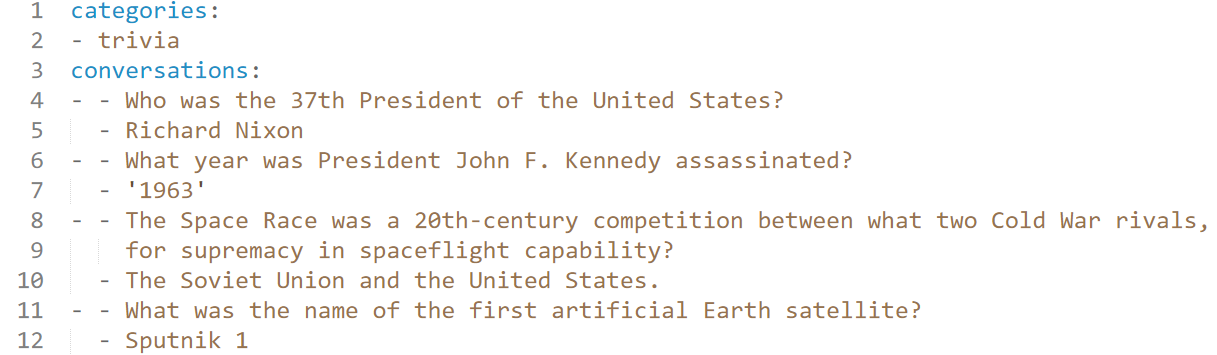
\includegraphics[width=1.0\columnwidth]{yaml-train}%
    \caption{\captionstyle{Example training file in the YAML format.}}%
    \label{fig:yaml-train}%
\end{figure}



\begin{lstlisting}[caption={\captionstyle{Writing scraped data to a file in the YAML format.}}, label={lst:write-file}]
# open out file
with open(out_file, 'w+', encoding="utf-8") as outfile:
    # write data
    yaml.dump(final_data, outfile)    
\end{lstlisting}

The resulting program worked well, however it was slow as only one question was processed at a time. To improve its performance, multithreading was implemented. This was achieved with a \texttt{ThreadPoolExecutor}. It allows the creation of asynchronous tasks. \cref{lst:threads} summarises the process. A \texttt{ThreadPoolExecutor} is created and its maximum number of threads is set. Threads are created and started and they are instructed to execute the \texttt{crawl\_pages} function. For each thread a suitable starting and ending page is calculated so that the work is split evenly. For example, if 10 pages were to be crawled with 2 threads, each thread will be assigned 5 pages. Additionally, thread 1 will start at page 1 and stop at page 5, while thread 2 will start at page 6 and stop at page 10.

\begin{lstlisting}[caption={\captionstyle{Multithreaded optimisation of the web crawler.}}, label={lst:threads}]
        with ThreadPoolExecutor(max_workers=workers) as executor:
            for i in range(workers):
                executor.submit(func, (i * num_pages + 1))
\end{lstlisting}

\cref{fig:crawlflow} summarises how one thread of the web crawler operates. When multiple threads are used, the same process occurs for each thread simultaneously.

\begin{figure}[htb]
	\centering
	\def\svgscale{0.7}
	\def\svgwidth{\columnwidth}
	%LaTeX with PSTricks extensions
%%Creator: inkscape 0.92.4
%%Please note this file requires PSTricks extensions
\psset{xunit=.5pt,yunit=.5pt,runit=.5pt}
\begin{pspicture}(537.33333333,561.33333333)
{
\newrgbcolor{curcolor}{0.7647059 0.18431373 0.02352941}
\pscustom[linewidth=1.33270017,linecolor=curcolor]
{
\newpath
\moveto(395.28610015,532.01394285)
\curveto(395.28610015,518.76540372)(353.74431125,508.02534049)(302.49991579,508.02533973)
\curveto(251.25551513,508.02533859)(209.71371811,518.76540237)(209.71371811,532.01394285)
\curveto(209.71371811,545.26248332)(251.25551513,556.00254711)(302.49991579,556.00254597)
\curveto(353.74431125,556.00254521)(395.28610015,545.26248198)(395.28610015,532.01394285)
\closepath
}
}
{
\newrgbcolor{curcolor}{1 1 1}
\pscustom[linestyle=none,fillstyle=solid,fillcolor=curcolor]
{
\newpath
\moveto(238.84005365,533.59079369)
\curveto(238.84005365,534.77773201)(239.07691889,535.81630081)(239.55064938,536.7065001)
\curveto(240.02959517,537.60190581)(240.71677092,538.28387514)(241.61217663,538.7524081)
\curveto(242.50758233,539.22613859)(243.55656397,539.46300383)(244.75912153,539.46300383)
\curveto(245.97728945,539.46300383)(247.11216361,539.23915018)(248.16374401,538.79144289)
\lineto(247.64836219,537.6201327)
\curveto(246.61760746,538.05741829)(245.62589195,538.27606108)(244.67321567,538.27606108)
\curveto(243.28325382,538.27606108)(242.19783172,537.86219548)(241.41694938,537.03446429)
\curveto(240.63607592,536.20673309)(240.2456392,535.0588429)(240.2456392,533.59079369)
\curveto(240.2456392,532.04985468)(240.62046112,530.88113882)(241.37010497,530.08464612)
\curveto(242.12495523,529.28815341)(243.23119855,528.88990706)(244.68883492,528.88990706)
\curveto(245.48013009,528.88990706)(246.25320281,528.98100601)(247.00805307,529.16320389)
\lineto(247.00805307,532.67716109)
\lineto(244.45457288,532.67716109)
\lineto(244.45457288,533.86410384)
\lineto(248.33554238,533.86410384)
\lineto(248.33554238,528.31204827)
\curveto(247.7316604,528.11942867)(247.11737002,527.97366681)(246.49267126,527.87476269)
\curveto(245.86796361,527.77584968)(245.1443474,527.72639318)(244.32182262,527.72639318)
\curveto(242.5934793,527.72639318)(241.24776309,528.23917178)(240.28467398,529.26472899)
\curveto(239.32159376,530.29548372)(238.84005365,531.73750529)(238.84005365,533.59079369)
\closepath
}
}
{
\newrgbcolor{curcolor}{1 1 1}
\pscustom[linestyle=none,fillstyle=solid,fillcolor=curcolor]
{
\newpath
\moveto(250.41267555,532.091506)
\curveto(250.41267555,533.47105502)(250.75105701,534.56688995)(251.42781992,535.37901079)
\curveto(252.10978926,536.19112273)(253.02341742,536.59717871)(254.16870441,536.59717871)
\curveto(255.24111047,536.59717871)(256.08966732,536.243178)(256.71437497,535.53517659)
\curveto(257.33907373,534.83239048)(257.65142312,533.90314752)(257.65142312,532.7474477)
\lineto(257.65142312,531.92751724)
\lineto(251.75579744,531.92751724)
\curveto(251.78182951,530.9227857)(252.034314,530.16013025)(252.51325091,529.63955091)
\curveto(252.99739423,529.11896268)(253.67675591,528.85866857)(254.55133595,528.85866857)
\curveto(255.47277374,528.85866857)(256.38379869,529.05128373)(257.28441082,529.43651404)
\lineto(257.28441082,528.28080978)
\curveto(256.82629957,528.08299265)(256.39161276,527.9424372)(255.98035037,527.85914344)
\curveto(255.5742944,527.77065215)(255.08234145,527.7264065)(254.50449154,527.7264065)
\curveto(253.23946589,527.7264065)(252.23994076,528.11164126)(251.50591615,528.88211077)
\curveto(250.77708908,529.65257139)(250.41267555,530.72237424)(250.41267555,532.09151933)
\closepath
\moveto(251.7870226,532.98170973)
\lineto(256.26147014,532.98170973)
\curveto(256.26147014,533.7990281)(256.07926338,534.4237313)(255.71484984,534.85581935)
\curveto(255.35043631,535.29311382)(254.82984808,535.51176105)(254.15308516,535.51176105)
\curveto(253.4659183,535.51176105)(252.91670367,535.2879074)(252.50544128,534.84020011)
\curveto(252.09937643,534.39249281)(251.85990353,533.77299602)(251.7870226,532.98170973)
\closepath
}
}
{
\newrgbcolor{curcolor}{1 1 1}
\pscustom[linestyle=none,fillstyle=solid,fillcolor=curcolor]
{
\newpath
\moveto(258.72123485,535.43366482)
\lineto(258.72123485,536.05836803)
\lineto(259.9472124,536.59717871)
\lineto(260.4938327,538.42443059)
\lineto(261.24347655,538.42443059)
\lineto(261.24347655,536.44099957)
\lineto(263.72667013,536.44099957)
\lineto(263.72667013,535.43366482)
\lineto(261.24347655,535.43366482)
\lineto(261.24347655,530.39699105)
\curveto(261.24347655,529.88161813)(261.36581398,529.48597499)(261.61048885,529.21006163)
\curveto(261.85516372,528.93414827)(262.19094197,528.79619159)(262.6178236,528.79619159)
\curveto(262.84687922,528.79619159)(263.06812522,528.8118286)(263.2815616,528.84310263)
\curveto(263.49500686,528.87952977)(263.66419759,528.91595691)(263.78913378,528.95238405)
\lineto(263.78913378,527.96066854)
\curveto(263.64857834,527.89296737)(263.44034394,527.83830445)(263.16443058,527.79667978)
\curveto(262.89373252,527.74985759)(262.64905765,527.72644649)(262.43040598,527.72644649)
\curveto(260.77494359,527.72644649)(259.9472124,528.59842777)(259.9472124,530.34239033)
\lineto(259.9472124,535.43371813)
\closepath
}
}
{
\newrgbcolor{curcolor}{1 1 1}
\pscustom[linestyle=none,fillstyle=solid,fillcolor=curcolor]
{
\newpath
\moveto(269.18501023,532.10712524)
\curveto(269.18501023,533.53873842)(269.5285981,534.64498174)(270.21577385,535.4258552)
\curveto(270.90815601,536.20673754)(271.8920619,536.59717871)(273.1674915,536.59717871)
\curveto(273.57875389,536.59717871)(273.99001628,536.55293306)(274.40127867,536.46444177)
\curveto(274.81254106,536.37595048)(275.13530771,536.27183106)(275.36957863,536.1520835)
\lineto(274.97132784,535.0510466)
\curveto(274.68500165,535.16557885)(274.37264782,535.25928544)(274.03426637,535.33216637)
\curveto(273.69588491,535.4102626)(273.39654712,535.44931072)(273.13625301,535.44931072)
\curveto(271.39749686,535.44931072)(270.52811879,534.34046419)(270.52811879,532.12277114)
\curveto(270.52811879,531.07118186)(270.7389564,530.26427189)(271.16063162,529.70204122)
\curveto(271.58751325,529.13981056)(272.21742287,528.85869523)(273.05036048,528.85869523)
\curveto(273.76356831,528.85869523)(274.49499414,529.01226671)(275.24463799,529.31940968)
\lineto(275.24463799,528.17151504)
\curveto(274.67198561,527.8747849)(273.95097261,527.72641983)(273.08159897,527.72641983)
\curveto(271.84260539,527.72641983)(270.88212394,528.10644817)(270.2001546,528.86650485)
\curveto(269.52339169,529.63176794)(269.18501023,530.71198363)(269.18501023,532.1071519)
\closepath
}
}
{
\newrgbcolor{curcolor}{1 1 1}
\pscustom[linestyle=none,fillstyle=solid,fillcolor=curcolor]
{
\newpath
\moveto(276.80638934,532.1695889)
\curveto(276.80638934,533.56476606)(277.15518363,534.65018816)(277.85277221,535.4258552)
\curveto(278.5503519,536.20673754)(279.51863854,536.59717871)(280.75763212,536.59717871)
\curveto(281.95498327,536.59717871)(282.90505634,536.19892791)(283.60785133,535.40242633)
\curveto(284.31584386,534.60593363)(284.66984012,533.52832115)(284.66984012,532.1695889)
\curveto(284.66984012,530.77442063)(284.31844706,529.68379211)(283.61566095,528.89770336)
\curveto(282.91286596,528.1168299)(281.94197167,527.72639318)(280.70297809,527.72639318)
\curveto(279.937715,527.72639318)(279.25834887,527.90599674)(278.66487972,528.26520386)
\curveto(278.07141056,528.62440209)(277.61329487,529.13977946)(277.29053266,529.81133596)
\curveto(276.96777045,530.48289247)(276.80638934,531.26897678)(276.80638934,532.1695889)
\closepath
\moveto(278.1494979,532.1695889)
\curveto(278.1494979,531.07635718)(278.36814514,530.24341957)(278.8054396,529.67077608)
\curveto(279.24273407,529.09813258)(279.88565973,528.81181083)(280.73421658,528.81181083)
\curveto(281.58276455,528.81181083)(282.22568577,529.09552937)(282.66298024,529.66296645)
\curveto(283.10548112,530.23560995)(283.32673156,531.07115076)(283.32673156,532.1695889)
\curveto(283.32673156,533.25761421)(283.10548112,534.08274219)(282.66298024,534.64497286)
\curveto(282.22568577,535.21241882)(281.57755814,535.4961418)(280.71859734,535.4961418)
\curveto(279.87004048,535.4961418)(279.22971803,535.21762524)(278.79762998,534.6605921)
\curveto(278.36554193,534.10356785)(278.1494979,533.27323345)(278.1494979,532.1695889)
\closepath
}
}
{
\newrgbcolor{curcolor}{1 1 1}
\pscustom[linestyle=none,fillstyle=solid,fillcolor=curcolor]
{
\newpath
\moveto(286.93439091,527.88257231)
\lineto(286.93439091,536.44099957)
\lineto(287.9885834,536.44099957)
\lineto(288.19941656,535.26967606)
\lineto(288.2619202,535.26967606)
\curveto(288.52742073,535.69135128)(288.89963945,536.01672115)(289.37857635,536.24578565)
\curveto(289.85752214,536.48004769)(290.3911264,536.59717871)(290.97938915,536.59717871)
\curveto(292.01014388,536.59717871)(292.78581536,536.34729742)(293.30640359,535.84753486)
\curveto(293.82699182,535.35297871)(294.08728593,534.55908477)(294.08728593,533.46585305)
\lineto(294.08728593,527.88257231)
\lineto(292.79102178,527.88257231)
\lineto(292.79102178,533.41899531)
\curveto(292.79102178,534.11658389)(292.63224388,534.63717212)(292.31468808,534.98075999)
\curveto(291.99713229,535.32434787)(291.49997293,535.4961418)(290.82321001,535.4961418)
\curveto(289.9278043,535.4961418)(289.27186705,535.2540657)(288.85539824,534.7699135)
\curveto(288.43892944,534.28577018)(288.23069504,533.48667427)(288.23069504,532.37262577)
\lineto(288.23069504,527.88257231)
\closepath
}
}
{
\newrgbcolor{curcolor}{1 1 1}
\pscustom[linestyle=none,fillstyle=solid,fillcolor=curcolor]
{
\newpath
\moveto(295.59434327,535.43366482)
\lineto(295.59434327,536.01931991)
\lineto(297.12485613,536.48785731)
\lineto(297.12485613,536.96419101)
\curveto(297.12485613,539.06736069)(298.0436907,540.11894553)(299.88135986,540.11894553)
\curveto(300.33427357,540.11894553)(300.86527463,540.02784215)(301.47436303,539.84563538)
\lineto(301.13857589,538.80706213)
\curveto(300.63881333,538.96844324)(300.21193614,539.04913379)(299.85794432,539.04913379)
\curveto(299.3685857,539.04913379)(299.00677537,538.88514948)(298.77251333,538.55718085)
\curveto(298.5382513,538.23441864)(298.42112028,537.71383485)(298.42112028,536.9954295)
\lineto(298.42112028,536.44099957)
\lineto(300.59977854,536.44099957)
\lineto(300.59977854,535.43366482)
\lineto(298.42112028,535.43366482)
\lineto(298.42112028,527.88257231)
\lineto(297.12485613,527.88257231)
\lineto(297.12485613,535.43366482)
\closepath
\moveto(302.0522085,538.76021772)
\curveto(302.0522085,539.05694786)(302.12508943,539.27298744)(302.27085129,539.40833647)
\curveto(302.41662203,539.5489008)(302.5988288,539.61918296)(302.81747159,539.61918296)
\curveto(303.02570155,539.61918296)(303.20530511,539.5489008)(303.35628227,539.40833647)
\curveto(303.50725055,539.26778103)(303.58273468,539.05174144)(303.58273468,538.76021772)
\curveto(303.58273468,538.46868512)(303.50725055,538.25003788)(303.35628227,538.10427602)
\curveto(303.20530511,537.96371169)(303.02570155,537.89342953)(302.81747159,537.89342953)
\curveto(302.5988288,537.89342953)(302.41662203,537.96371169)(302.27085129,538.10427602)
\curveto(302.12508943,538.25003788)(302.0522085,538.46868512)(302.0522085,538.76021772)
\closepath
\moveto(302.16148991,527.88257231)
\lineto(302.16148991,536.44099957)
\lineto(303.45775406,536.44099957)
\lineto(303.45775406,527.88257231)
\closepath
}
}
{
\newrgbcolor{curcolor}{1 1 1}
\pscustom[linestyle=none,fillstyle=solid,fillcolor=curcolor]
{
\newpath
\moveto(305.13667641,526.43012903)
\curveto(305.13667641,526.95071725)(305.30326393,527.40102331)(305.63643898,527.78104721)
\curveto(305.96961402,528.16107999)(306.43814254,528.4187709)(307.04202452,528.55411993)
\curveto(306.82338173,528.65303294)(306.6385762,528.80660886)(306.48760792,529.01484771)
\curveto(306.34183718,529.22307766)(306.26895181,529.46514932)(306.26895181,529.74106268)
\curveto(306.26895181,530.05341207)(306.35224557,530.32671777)(306.51883309,530.56097981)
\curveto(306.68542061,530.79524185)(306.94831793,531.0216987)(307.30752505,531.24035038)
\curveto(306.86502417,531.42255715)(306.50321829,531.73230332)(306.2221074,532.1695889)
\curveto(305.94619404,532.60688337)(305.80823736,533.10664593)(305.80823736,533.6688766)
\curveto(305.80823736,534.60593363)(306.08935269,535.32694663)(306.65158335,535.83191561)
\curveto(307.21381402,536.34209101)(308.01031116,536.59717871)(309.04107478,536.59717871)
\curveto(309.48878208,536.59717871)(309.89223485,536.54511899)(310.25143308,536.44099957)
\lineto(313.21097368,536.44099957)
\lineto(313.21097368,535.62108245)
\lineto(311.62578013,535.43366482)
\curveto(311.77155088,535.25145805)(311.90169794,535.0119896)(312.0162213,534.71525946)
\curveto(312.13075356,534.42372686)(312.18801968,534.09315502)(312.18801968,533.72354396)
\curveto(312.18801968,532.88539993)(311.90169794,532.21644664)(311.32905444,531.71668407)
\curveto(310.75641095,531.21692151)(309.97032663,530.96704023)(308.9708015,530.96704023)
\curveto(308.71571381,530.96704023)(308.47624091,530.98787477)(308.25238282,531.02954387)
\curveto(307.70056499,530.73802014)(307.42465607,530.37100784)(307.42465607,529.92850696)
\curveto(307.42465607,529.69424493)(307.52096587,529.51984778)(307.71358547,529.40531553)
\curveto(307.90619618,529.29599858)(308.23676802,529.2413401)(308.70530098,529.2413401)
\lineto(310.22020792,529.2413401)
\curveto(311.14685212,529.2413401)(311.85745229,529.04611729)(312.35200844,528.65567168)
\curveto(312.85177101,528.26523495)(313.10165229,527.69779787)(313.10165229,526.95336044)
\curveto(313.10165229,526.00589058)(312.72162395,525.28487758)(311.96156727,524.79032143)
\curveto(311.20151059,524.29055886)(310.09265962,524.04067758)(308.63501437,524.04067758)
\curveto(307.51575945,524.04067758)(306.6515878,524.24891198)(306.04249939,524.66538078)
\curveto(305.43861741,525.08184959)(305.13667641,525.67011233)(305.13667641,526.43016901)
\closepath
\moveto(306.38608283,526.44572162)
\curveto(306.38608283,525.98240396)(306.58130563,525.63101091)(306.97175124,525.39154245)
\curveto(307.36218797,525.15206512)(307.92181543,525.03232645)(308.65063361,525.03232645)
\curveto(309.73865892,525.03232645)(310.54296569,525.19631076)(311.06355391,525.52427939)
\curveto(311.58934855,525.84705049)(311.85224588,526.28694816)(311.85224588,526.84397241)
\curveto(311.85224588,527.30729007)(311.70908278,527.63005228)(311.42275659,527.81225905)
\curveto(311.1364304,527.9892594)(310.59762416,528.07775958)(309.80633788,528.07775958)
\lineto(308.25238282,528.07775958)
\curveto(307.66412008,528.07775958)(307.2060044,527.93719969)(306.87803577,527.65607992)
\curveto(306.55006714,527.37496903)(306.38608283,526.97151626)(306.38608283,526.44572162)
\closepath
\moveto(307.08888226,533.70008843)
\curveto(307.08888226,533.10141286)(307.25807299,532.64850359)(307.59645445,532.34136063)
\curveto(307.93483591,532.03421766)(308.40596319,531.88064618)(309.00983629,531.88064618)
\curveto(310.27486195,531.88064618)(310.90737478,532.49493655)(310.90737478,533.7235173)
\curveto(310.90737478,535.00935974)(310.26705677,535.65228096)(308.98642075,535.65228096)
\curveto(308.37733235,535.65228096)(307.90880383,535.48829664)(307.5808352,535.16032801)
\curveto(307.25286658,534.83235939)(307.08888226,534.34561286)(307.08888226,533.70008843)
\closepath
}
}
{
\newrgbcolor{curcolor}{1 1 1}
\pscustom[linestyle=none,fillstyle=solid,fillcolor=curcolor]
{
\newpath
\moveto(314.88985605,530.84209959)
\lineto(314.88985605,536.44099957)
\lineto(316.20173945,536.44099957)
\lineto(316.20173945,530.88895732)
\curveto(316.20173945,530.19136875)(316.36051735,529.67078052)(316.67807315,529.32719264)
\curveto(316.99562894,528.98360477)(317.4927883,528.81181083)(318.16955122,528.81181083)
\curveto(319.06495693,528.81181083)(319.71829097,529.0564857)(320.12955336,529.54583544)
\curveto(320.54602217,530.03518517)(320.75425657,530.83428552)(320.75425657,531.94313649)
\lineto(320.75425657,536.44099957)
\lineto(322.05052072,536.44099957)
\lineto(322.05052072,527.88257231)
\lineto(320.98072231,527.88257231)
\lineto(320.79330468,529.03045362)
\lineto(320.72307138,529.03045362)
\curveto(320.45757086,528.6087784)(320.08795091,528.28601619)(319.61421153,528.06216699)
\curveto(319.14568746,527.83831778)(318.60948443,527.72639318)(318.00560244,527.72639318)
\curveto(316.96443487,527.72639318)(316.18355698,527.97367125)(315.66296875,528.4682274)
\curveto(315.14758694,528.96278355)(314.88989603,529.75407428)(314.88989603,530.84209959)
\closepath
}
}
{
\newrgbcolor{curcolor}{1 1 1}
\pscustom[linestyle=none,fillstyle=solid,fillcolor=curcolor]
{
\newpath
\moveto(324.7914052,527.88257231)
\lineto(324.7914052,536.44099957)
\lineto(325.86120361,536.44099957)
\lineto(326.00957312,534.85581935)
\lineto(326.07207676,534.85581935)
\curveto(326.38963256,535.4128436)(326.77226411,535.842324)(327.2199714,536.14426055)
\curveto(327.66766981,536.44620599)(328.15962276,536.59717871)(328.69583023,536.59717871)
\curveto(329.07585413,536.59717871)(329.41683879,536.5659491)(329.71878423,536.50348988)
\lineto(329.53917623,535.30092788)
\curveto(329.18517552,535.37902411)(328.87282614,535.41807223)(328.60212808,535.41807223)
\curveto(327.90974592,535.41807223)(327.31627676,535.1369569)(326.82172061,534.57472623)
\curveto(326.33237088,534.01249557)(326.08769601,533.31230822)(326.08769601,532.4741642)
\lineto(326.08769601,527.88259896)
\closepath
}
}
{
\newrgbcolor{curcolor}{1 1 1}
\pscustom[linestyle=none,fillstyle=solid,fillcolor=curcolor]
{
\newpath
\moveto(330.67923459,530.24863487)
\curveto(330.67923459,531.97697819)(332.06139127,532.88279673)(334.82570462,532.96609049)
\lineto(336.27813458,533.01300153)
\lineto(336.27813458,533.54398926)
\curveto(336.27813458,534.21554576)(336.13237272,534.71010191)(335.84084899,535.02765771)
\curveto(335.5545228,535.35042881)(335.09380391,535.51181436)(334.45869232,535.51181436)
\curveto(333.74548449,535.51181436)(332.93857452,535.29316713)(332.0379624,534.85587266)
\lineto(331.6397116,535.84758817)
\curveto(332.06138682,536.07664379)(332.52210572,536.25624735)(333.02186828,536.38639885)
\curveto(333.52683726,536.51654146)(334.03180624,536.58161277)(334.53677522,536.58161277)
\curveto(335.55712601,536.58161277)(336.31197628,536.35515591)(336.80132601,535.9022422)
\curveto(337.29588216,535.44933737)(337.54316023,534.7231224)(337.54316023,533.72359727)
\lineto(337.54316023,527.88262562)
\lineto(336.58268322,527.88262562)
\lineto(336.32499231,529.10079354)
\lineto(336.26248868,529.10079354)
\curveto(335.83560704,528.56458607)(335.40872541,528.20017697)(334.98184377,528.00756626)
\curveto(334.56017744,527.82015308)(334.03178403,527.72644649)(333.39666355,527.72644649)
\curveto(332.5481067,527.72644649)(331.88175661,527.94509372)(331.39761329,528.38238818)
\curveto(330.91867639,528.81967376)(330.67920793,529.44177376)(330.67920793,530.24868818)
\closepath
\moveto(332.0379624,530.23304228)
\curveto(332.0379624,529.76450932)(332.17852228,529.40790541)(332.45964206,529.16323054)
\curveto(332.74595936,528.91855568)(333.14420571,528.79621824)(333.65438111,528.79621824)
\curveto(334.46128664,528.79621824)(335.09379947,529.01746868)(335.5519196,529.45996956)
\curveto(336.01523725,529.90247044)(336.24689608,530.52196723)(336.24689608,531.31845994)
\lineto(336.24689608,532.09153265)
\lineto(334.95064526,532.03689195)
\curveto(333.91988164,532.00046481)(333.17544421,531.8390837)(332.71733296,531.55274863)
\curveto(332.26441925,531.27163774)(332.0379624,530.83174451)(332.0379624,530.23306893)
\closepath
}
}
{
\newrgbcolor{curcolor}{1 1 1}
\pscustom[linestyle=none,fillstyle=solid,fillcolor=curcolor]
{
\newpath
\moveto(339.08930567,535.43366482)
\lineto(339.08930567,536.05836803)
\lineto(340.31528321,536.59717871)
\lineto(340.86189019,538.42443059)
\lineto(341.61153403,538.42443059)
\lineto(341.61153403,536.44099957)
\lineto(344.09474094,536.44099957)
\lineto(344.09474094,535.43366482)
\lineto(341.61153403,535.43366482)
\lineto(341.61153403,530.39699105)
\curveto(341.61153403,529.88161813)(341.73387147,529.48597499)(341.97854633,529.21006163)
\curveto(342.22323009,528.93414827)(342.55900834,528.79619159)(342.98588109,528.79619159)
\curveto(343.21494559,528.79619159)(343.43619603,528.8118286)(343.64963241,528.84310263)
\curveto(343.86307767,528.87952977)(344.0322684,528.91595691)(344.1572046,528.95238405)
\lineto(344.1572046,527.96066854)
\curveto(344.01664915,527.89296737)(343.80841475,527.83830445)(343.53250139,527.79667978)
\curveto(343.26179445,527.74985759)(343.01711958,527.72644649)(342.79847679,527.72644649)
\curveto(341.1430144,527.72644649)(340.31528321,528.59842777)(340.31528321,530.34239033)
\lineto(340.31528321,535.43371813)
\closepath
}
}
{
\newrgbcolor{curcolor}{1 1 1}
\pscustom[linestyle=none,fillstyle=solid,fillcolor=curcolor]
{
\newpath
\moveto(345.76581369,538.76021772)
\curveto(345.76581369,539.05694786)(345.83869462,539.27298744)(345.98445648,539.40833647)
\curveto(346.13022722,539.5489008)(346.31243399,539.61918296)(346.53107678,539.61918296)
\curveto(346.73931562,539.61918296)(346.91891919,539.5489008)(347.06988746,539.40833647)
\curveto(347.22085574,539.26778103)(347.29633987,539.05174144)(347.29633987,538.76021772)
\curveto(347.29633987,538.46868512)(347.22085574,538.25003788)(347.06988746,538.10427602)
\curveto(346.91891919,537.96371169)(346.73931562,537.89342953)(346.53107678,537.89342953)
\curveto(346.31243399,537.89342953)(346.13022722,537.96371169)(345.98445648,538.10427602)
\curveto(345.83869462,538.25003788)(345.76581369,538.46868512)(345.76581369,538.76021772)
\closepath
\moveto(345.8750951,527.88257231)
\lineto(345.8750951,536.44099957)
\lineto(347.17135925,536.44099957)
\lineto(347.17135925,527.88257231)
\closepath
}
}
{
\newrgbcolor{curcolor}{1 1 1}
\pscustom[linestyle=none,fillstyle=solid,fillcolor=curcolor]
{
\newpath
\moveto(349.45937889,532.1695889)
\curveto(349.45937889,533.56476606)(349.80816874,534.65018816)(350.50574843,535.4258552)
\curveto(351.20333701,536.20673754)(352.17162809,536.59717871)(353.41062167,536.59717871)
\curveto(354.60797282,536.59717871)(355.55804144,536.19892791)(356.26082755,535.40242633)
\curveto(356.96882896,534.60593363)(357.32282967,533.52832115)(357.32282967,532.1695889)
\curveto(357.32282967,530.77442063)(356.97143217,529.68379211)(356.26863717,528.89770336)
\curveto(355.56585107,528.1168299)(354.59495678,527.72639318)(353.35595431,527.72639318)
\curveto(352.5907001,527.72639318)(351.91133842,527.90599674)(351.31786926,528.26520386)
\curveto(350.72440011,528.62440209)(350.26628442,529.13977946)(349.94352221,529.81133596)
\curveto(349.62076,530.48289247)(349.45937889,531.26897678)(349.45937889,532.1695889)
\closepath
\moveto(350.80248745,532.1695889)
\curveto(350.80248745,531.07635718)(351.02113468,530.24341957)(351.45842915,529.67077608)
\curveto(351.89571473,529.09813258)(352.53863595,528.81181083)(353.3871928,528.81181083)
\curveto(354.23574966,528.81181083)(354.87867532,529.09552937)(355.31596978,529.66296645)
\curveto(355.75846178,530.23560995)(355.97970778,531.07115076)(355.97970778,532.1695889)
\curveto(355.97970778,533.25761421)(355.75846178,534.08274219)(355.31596978,534.64497286)
\curveto(354.87867532,535.21241882)(354.23054324,535.4961418)(353.37157356,535.4961418)
\curveto(352.5230167,535.4961418)(351.88269869,535.21762524)(351.45061953,534.6605921)
\curveto(351.01853148,534.10356785)(350.80248745,533.27323345)(350.80248745,532.1695889)
\closepath
}
}
{
\newrgbcolor{curcolor}{1 1 1}
\pscustom[linestyle=none,fillstyle=solid,fillcolor=curcolor]
{
\newpath
\moveto(359.58738045,527.88257231)
\lineto(359.58738045,536.44099957)
\lineto(360.64155962,536.44099957)
\lineto(360.85239279,535.26967606)
\lineto(360.91489642,535.26967606)
\curveto(361.18039695,535.69135128)(361.55261567,536.01672115)(362.03155257,536.24578565)
\curveto(362.51048948,536.48004769)(363.0440893,536.59717871)(363.63235204,536.59717871)
\curveto(364.66311566,536.59717871)(365.43879159,536.34729742)(365.95937981,535.84753486)
\curveto(366.47995915,535.35297871)(366.74024882,534.55908477)(366.74024882,533.46585305)
\lineto(366.74024882,527.88257231)
\lineto(365.443998,527.88257231)
\lineto(365.443998,533.41899531)
\curveto(365.443998,534.11658389)(365.28521566,534.63717212)(364.96765098,534.98075999)
\curveto(364.65009518,535.32434787)(364.15293582,535.4961418)(363.47617291,535.4961418)
\curveto(362.5807672,535.4961418)(361.92482994,535.2540657)(361.50836114,534.7699135)
\curveto(361.09189233,534.28577018)(360.88365793,533.48667427)(360.88365793,532.37262577)
\lineto(360.88365793,527.88257231)
\closepath
}
}
{
\newrgbcolor{curcolor}{0.24705882 0.31764707 0.70980394}
\pscustom[linewidth=1.33270017,linecolor=curcolor]
{
\newpath
\moveto(362.47142359,429.39601618)
\lineto(362.47142359,477.37322242)
\lineto(242.528408,477.37322242)
\lineto(242.528408,429.39601618)
\closepath
}
}
{
\newrgbcolor{curcolor}{1 1 1}
\pscustom[linestyle=none,fillstyle=solid,fillcolor=curcolor]
{
\newpath
\moveto(252.68503596,449.62027439)
\lineto(252.68503596,450.90090597)
\curveto(253.15356892,450.70308884)(253.66374431,450.54691415)(254.21556215,450.43238189)
\curveto(254.76737998,450.31785852)(255.31399584,450.26059684)(255.85540973,450.26059684)
\curveto(256.74040261,450.26059684)(257.40675269,450.42718436)(257.85445999,450.7603594)
\curveto(258.3021584,451.09873198)(258.52600761,451.56725605)(258.52600761,452.16593162)
\curveto(258.52600761,452.56158365)(258.44531705,452.88435031)(258.28393595,453.13423159)
\curveto(258.12776126,453.3893104)(257.86226517,453.62357244)(257.48744769,453.8370177)
\curveto(257.11782774,454.05045407)(256.55298942,454.29252573)(255.79293274,454.56323268)
\curveto(254.73093951,454.94326546)(253.97088728,455.39357152)(253.51277604,455.91415086)
\curveto(253.05986233,456.43473909)(252.83340547,457.11410521)(252.83340547,457.95224924)
\curveto(252.83340547,458.8320357)(253.16397731,459.53222304)(253.82512098,460.05281127)
\curveto(254.48626465,460.57339949)(255.36084914,460.83369361)(256.44887444,460.83369361)
\curveto(257.5837486,460.83369361)(258.62752382,460.62545921)(259.5802001,460.2089904)
\lineto(259.16633006,459.05328614)
\curveto(258.2240755,459.44892928)(257.30784413,459.64675085)(256.41763595,459.64675085)
\curveto(255.71484984,459.64675085)(255.16563077,459.49578258)(254.76997875,459.19384603)
\curveto(254.3743356,458.89190947)(254.17651403,458.47283746)(254.17651403,457.93662999)
\curveto(254.17651403,457.54098685)(254.24939496,457.21562143)(254.39515682,456.96053373)
\curveto(254.54092757,456.71065245)(254.78560688,456.47898918)(255.12919475,456.26554392)
\curveto(255.47798015,456.05731396)(256.00897677,455.82565513)(256.72218459,455.57056743)
\curveto(257.91952685,455.14368579)(258.74205163,454.68557011)(259.18975893,454.19622038)
\curveto(259.64267264,453.70687064)(259.86912949,453.0717546)(259.86912949,452.29087226)
\curveto(259.86912949,451.28614072)(259.50471596,450.50265961)(258.77588889,449.94042895)
\curveto(258.0470707,449.37819829)(257.0579584,449.09708295)(255.80855199,449.09708295)
\curveto(254.45502616,449.09708295)(253.41385415,449.2714801)(252.68503596,449.62027439)
\closepath
}
}
{
\newrgbcolor{curcolor}{1 1 1}
\pscustom[linestyle=none,fillstyle=solid,fillcolor=curcolor]
{
\newpath
\moveto(260.87646425,456.8043546)
\lineto(260.87646425,457.4290578)
\lineto(262.10244179,457.96786848)
\lineto(262.64904877,459.79512036)
\lineto(263.39869261,459.79512036)
\lineto(263.39869261,457.81168935)
\lineto(265.88189952,457.81168935)
\lineto(265.88189952,456.8043546)
\lineto(263.39869261,456.8043546)
\lineto(263.39869261,451.76768083)
\curveto(263.39869261,451.2523079)(263.52103005,450.85666476)(263.76570491,450.5807514)
\curveto(264.01038867,450.30483804)(264.34616692,450.16688136)(264.77303967,450.16688136)
\curveto(265.00210417,450.16688136)(265.22335461,450.18251838)(265.43679099,450.21379241)
\curveto(265.65023625,450.25021955)(265.81942698,450.28664669)(265.94436318,450.32307382)
\lineto(265.94436318,449.33135832)
\curveto(265.80380773,449.26365715)(265.59557333,449.20899423)(265.31965997,449.16736956)
\curveto(265.04895303,449.12054736)(264.80427816,449.09713626)(264.58563537,449.09713626)
\curveto(262.93017298,449.09713626)(262.10244179,449.96911754)(262.10244179,451.7130801)
\lineto(262.10244179,456.8044079)
\closepath
}
}
{
\newrgbcolor{curcolor}{1 1 1}
\pscustom[linestyle=none,fillstyle=solid,fillcolor=curcolor]
{
\newpath
\moveto(267.02197121,451.61932465)
\curveto(267.02197121,453.34766796)(268.40412789,454.2534865)(271.16844124,454.33678026)
\lineto(272.62088452,454.38369131)
\lineto(272.62088452,454.91467904)
\curveto(272.62088452,455.58623554)(272.47511822,456.08079169)(272.18358562,456.39834749)
\curveto(271.89726831,456.72111859)(271.43654942,456.88250413)(270.80142894,456.88250413)
\curveto(270.08823,456.88250413)(269.28132447,456.6638569)(268.38071234,456.22656244)
\lineto(267.98246155,457.21827794)
\curveto(268.40413677,457.44733356)(268.86485566,457.62693712)(269.36461823,457.75708862)
\curveto(269.86958721,457.88723124)(270.37455619,457.95230254)(270.87952517,457.95230254)
\curveto(271.89986708,457.95230254)(272.6547129,457.72584569)(273.14406263,457.27293198)
\curveto(273.63861878,456.82002715)(273.88589686,456.09381217)(273.88589686,455.09428704)
\lineto(273.88589686,449.25331539)
\lineto(272.92541984,449.25331539)
\lineto(272.66772894,450.47148332)
\lineto(272.6052253,450.47148332)
\curveto(272.17834366,449.93527584)(271.75146203,449.57086675)(271.32458039,449.37825604)
\curveto(270.90290517,449.19084285)(270.37451177,449.09713626)(269.73940017,449.09713626)
\curveto(268.89084332,449.09713626)(268.22449323,449.31578349)(267.74034991,449.75307796)
\curveto(267.26140412,450.19036354)(267.02193123,450.81246354)(267.02193123,451.61937796)
\closepath
\moveto(268.38071234,451.60373206)
\curveto(268.38071234,451.1351991)(268.52126779,450.77859519)(268.80237868,450.53392032)
\curveto(269.08870487,450.28924545)(269.48695566,450.16690802)(269.99713106,450.16690802)
\curveto(270.80403659,450.16690802)(271.43654498,450.38815846)(271.89465622,450.83065934)
\curveto(272.35798276,451.27316022)(272.58964603,451.89265701)(272.58964603,452.68914971)
\lineto(272.58964603,453.46222243)
\lineto(271.29338188,453.40758172)
\curveto(270.26262714,453.37115458)(269.51818971,453.20977348)(269.06006959,452.9234384)
\curveto(268.60716476,452.64232751)(268.38071234,452.20243428)(268.38071234,451.60375871)
\closepath
}
}
{
\newrgbcolor{curcolor}{1 1 1}
\pscustom[linestyle=none,fillstyle=solid,fillcolor=curcolor]
{
\newpath
\moveto(276.56431768,449.25326209)
\lineto(276.56431768,457.81168935)
\lineto(277.63411609,457.81168935)
\lineto(277.7824856,456.22650913)
\lineto(277.84498924,456.22650913)
\curveto(278.16254504,456.78353338)(278.54517659,457.21301378)(278.99288388,457.51495033)
\curveto(279.44058229,457.81689576)(279.93253524,457.96786848)(280.46874271,457.96786848)
\curveto(280.8487666,457.96786848)(281.18975127,457.93663887)(281.49169671,457.87417966)
\lineto(281.3120887,456.67161766)
\curveto(280.958088,456.74971389)(280.64573862,456.788762)(280.37504056,456.788762)
\curveto(279.6826584,456.788762)(279.08918924,456.50764667)(278.59463309,455.94541601)
\curveto(278.10528335,455.38318534)(277.86060849,454.682998)(277.86060849,453.84485397)
\lineto(277.86060849,449.25328874)
\closepath
}
}
{
\newrgbcolor{curcolor}{1 1 1}
\pscustom[linestyle=none,fillstyle=solid,fillcolor=curcolor]
{
\newpath
\moveto(281.96019413,456.8043546)
\lineto(281.96019413,457.4290578)
\lineto(283.18617167,457.96786848)
\lineto(283.73279197,459.79512036)
\lineto(284.48243582,459.79512036)
\lineto(284.48243582,457.81168935)
\lineto(286.9656294,457.81168935)
\lineto(286.9656294,456.8043546)
\lineto(284.48243582,456.8043546)
\lineto(284.48243582,451.76768083)
\curveto(284.48243582,451.2523079)(284.60477325,450.85666476)(284.84944812,450.5807514)
\curveto(285.09412299,450.30483804)(285.42990124,450.16688136)(285.85678287,450.16688136)
\curveto(286.08583849,450.16688136)(286.30708449,450.18251838)(286.52052087,450.21379241)
\curveto(286.73396613,450.25021955)(286.90315686,450.28664669)(287.02809306,450.32307382)
\lineto(287.02809306,449.33135832)
\curveto(286.88753761,449.26365715)(286.67930321,449.20899423)(286.40338985,449.16736956)
\curveto(286.13269179,449.12054736)(285.88801692,449.09713626)(285.66936525,449.09713626)
\curveto(284.01390286,449.09713626)(283.18617167,449.96911754)(283.18617167,451.7130801)
\lineto(283.18617167,456.8044079)
\closepath
}
}
{
\newrgbcolor{curcolor}{1 1 1}
\pscustom[linestyle=none,fillstyle=solid,fillcolor=curcolor]
{
\newpath
\moveto(292.4239695,453.47781502)
\curveto(292.4239695,454.9094282)(292.76755737,456.01567152)(293.45473312,456.79654497)
\curveto(294.14711528,457.57742731)(295.13102117,457.96786848)(296.40645077,457.96786848)
\curveto(296.81771316,457.96786848)(297.22897555,457.92362284)(297.64023794,457.83513154)
\curveto(298.05150033,457.74664025)(298.37426698,457.64252083)(298.6085379,457.52277328)
\lineto(298.21028711,456.42173638)
\curveto(297.92396092,456.53626863)(297.6116071,456.62997522)(297.27322564,456.70285615)
\curveto(296.93484418,456.78095238)(296.63550639,456.8200005)(296.37521228,456.8200005)
\curveto(294.63645613,456.8200005)(293.76707806,455.71115397)(293.76707806,453.49346092)
\curveto(293.76707806,452.44187164)(293.97791567,451.63496166)(294.39959089,451.072731)
\curveto(294.82647252,450.51050033)(295.45638215,450.229385)(296.28931975,450.229385)
\curveto(297.00252758,450.229385)(297.73395341,450.38295649)(298.48359726,450.69009945)
\lineto(298.48359726,449.54220481)
\curveto(297.91094488,449.24547468)(297.18993188,449.09710961)(296.32055825,449.09710961)
\curveto(295.08156466,449.09710961)(294.12108321,449.47713795)(293.43911387,450.23719462)
\curveto(292.76235096,451.00245772)(292.4239695,452.0826734)(292.4239695,453.47784167)
\closepath
}
}
{
\newrgbcolor{curcolor}{1 1 1}
\pscustom[linestyle=none,fillstyle=solid,fillcolor=curcolor]
{
\newpath
\moveto(300.52168231,449.25326209)
\lineto(300.52168231,457.81168935)
\lineto(301.59149405,457.81168935)
\lineto(301.73986356,456.22650913)
\lineto(301.8023672,456.22650913)
\curveto(302.11992299,456.78353338)(302.50255454,457.21301378)(302.95026184,457.51495033)
\curveto(303.39796025,457.81689576)(303.88991319,457.96786848)(304.42612066,457.96786848)
\curveto(304.80614456,457.96786848)(305.14712922,457.93663887)(305.44907466,457.87417966)
\lineto(305.26946666,456.67161766)
\curveto(304.91547484,456.74971389)(304.60312546,456.788762)(304.33241851,456.788762)
\curveto(303.64003635,456.788762)(303.04656719,456.50764667)(302.55201104,455.94541601)
\curveto(302.06266131,455.38318534)(301.81798644,454.682998)(301.81798644,453.84485397)
\lineto(301.81798644,449.25328874)
\closepath
}
}
{
\newrgbcolor{curcolor}{1 1 1}
\pscustom[linestyle=none,fillstyle=solid,fillcolor=curcolor]
{
\newpath
\moveto(306.40951169,451.61932465)
\curveto(306.40951169,453.34766796)(307.79166837,454.2534865)(310.55598172,454.33678026)
\lineto(312.00841168,454.38369131)
\lineto(312.00841168,454.91467904)
\curveto(312.00841168,455.58623554)(311.86264982,456.08079169)(311.5711261,456.39834749)
\curveto(311.28479991,456.72111859)(310.82408102,456.88250413)(310.18896942,456.88250413)
\curveto(309.4757616,456.88250413)(308.66885163,456.6638569)(307.7682395,456.22656244)
\lineto(307.36998871,457.21827794)
\curveto(307.79166393,457.44733356)(308.25238282,457.62693712)(308.75214539,457.75708862)
\curveto(309.25711437,457.88723124)(309.76208335,457.95230254)(310.26705233,457.95230254)
\curveto(311.28740312,457.95230254)(312.04225338,457.72584569)(312.53160312,457.27293198)
\curveto(313.02615927,456.82002715)(313.27343734,456.09381217)(313.27343734,455.09428704)
\lineto(313.27343734,449.25331539)
\lineto(312.31296033,449.25331539)
\lineto(312.05526942,450.47148332)
\lineto(311.99276578,450.47148332)
\curveto(311.56589303,449.93527584)(311.13901584,449.57086675)(310.7121342,449.37825604)
\curveto(310.29045898,449.19084285)(309.76206114,449.09713626)(309.12694066,449.09713626)
\curveto(308.27839269,449.09713626)(307.6120426,449.31578349)(307.1278904,449.75307796)
\curveto(306.64895349,450.19036354)(306.40948504,450.81246354)(306.40948504,451.61937796)
\closepath
\moveto(307.7682395,451.60373206)
\curveto(307.7682395,451.1351991)(307.90879939,450.77859519)(308.18991916,450.53392032)
\curveto(308.47623647,450.28924545)(308.87448282,450.16690802)(309.38465822,450.16690802)
\curveto(310.19157263,450.16690802)(310.82408546,450.38815846)(311.2821967,450.83065934)
\curveto(311.74552325,451.27316022)(311.97718652,451.89265701)(311.97718652,452.68914971)
\lineto(311.97718652,453.46222243)
\lineto(310.68092237,453.40758172)
\curveto(309.65015874,453.37115458)(308.90572131,453.20977348)(308.44761007,452.9234384)
\curveto(307.99469636,452.64232751)(307.7682395,452.20243428)(307.7682395,451.60375871)
\closepath
}
}
{
\newrgbcolor{curcolor}{1 1 1}
\pscustom[linestyle=none,fillstyle=solid,fillcolor=curcolor]
{
\newpath
\moveto(314.75710579,457.81168935)
\lineto(316.1158336,457.81168935)
\curveto(316.66766032,455.66167081)(317.08673233,454.02442644)(317.37304963,452.89995623)
\curveto(317.66458224,451.7754949)(317.83116976,451.01804587)(317.8728122,450.62760914)
\lineto(317.93531584,450.62760914)
\curveto(317.9925331,450.92433928)(318.08363648,451.30696638)(318.20862599,451.77549045)
\curveto(318.3387686,452.24922983)(318.4506932,452.62405175)(318.5443998,452.89995623)
\lineto(320.11396077,457.81168935)
\lineto(321.51954632,457.81168935)
\lineto(323.0500725,452.89995623)
\curveto(323.34159622,452.00455052)(323.5394178,451.25230346)(323.64353722,450.64321506)
\lineto(323.70604086,450.64321506)
\curveto(323.72683098,450.83062824)(323.78148945,451.11955764)(323.87001629,451.51000325)
\curveto(323.96372288,451.90043998)(324.50773553,454.00100201)(325.50205424,457.81168935)
\lineto(326.84517613,457.81168935)
\lineto(324.47911357,449.25326209)
\lineto(322.94077776,449.25326209)
\lineto(321.37120346,454.27430328)
\curveto(321.27229934,454.58145513)(321.0874938,455.27904371)(320.81678686,456.36706901)
\lineto(320.75428322,456.36706901)
\curveto(320.54605326,455.45604406)(320.36385094,454.75325351)(320.20767625,454.25869736)
\lineto(318.59125753,449.25326209)
\lineto(317.09196984,449.25326209)
\closepath
}
}
{
\newrgbcolor{curcolor}{1 1 1}
\pscustom[linestyle=none,fillstyle=solid,fillcolor=curcolor]
{
\newpath
\moveto(328.38344531,449.25326209)
\lineto(328.38344531,461.40372945)
\lineto(329.67970946,461.40372945)
\lineto(329.67970946,449.25326209)
\closepath
}
}
{
\newrgbcolor{curcolor}{1 1 1}
\pscustom[linestyle=none,fillstyle=solid,fillcolor=curcolor]
{
\newpath
\moveto(332.33470142,460.1309075)
\curveto(332.33470142,460.42763763)(332.40758235,460.64367722)(332.55334421,460.77902625)
\curveto(332.69910607,460.91959058)(332.88131284,460.98987274)(333.09996451,460.98987274)
\curveto(333.30819447,460.98987274)(333.48779359,460.91959058)(333.63876186,460.77902625)
\curveto(333.78973014,460.6384708)(333.86521428,460.42243122)(333.86521428,460.1309075)
\curveto(333.86521428,459.83937489)(333.78973014,459.62072766)(333.63876186,459.4749658)
\curveto(333.48779359,459.33440147)(333.30819447,459.26411931)(333.09996451,459.26411931)
\curveto(332.88131284,459.26411931)(332.69910607,459.33440147)(332.55334421,459.4749658)
\curveto(332.40758235,459.62072766)(332.33470142,459.83937489)(332.33470142,460.1309075)
\closepath
\moveto(332.44398283,449.25326209)
\lineto(332.44398283,457.81168935)
\lineto(333.74023365,457.81168935)
\lineto(333.74023365,449.25326209)
\closepath
}
}
{
\newrgbcolor{curcolor}{1 1 1}
\pscustom[linestyle=none,fillstyle=solid,fillcolor=curcolor]
{
\newpath
\moveto(336.50458699,449.25326209)
\lineto(336.50458699,457.81168935)
\lineto(337.55877948,457.81168935)
\lineto(337.76961265,456.64036584)
\lineto(337.83211629,456.64036584)
\curveto(338.09760793,457.06204106)(338.46982665,457.38741092)(338.94877243,457.61647543)
\curveto(339.42770934,457.85073746)(339.96130916,457.96786848)(340.5495719,457.96786848)
\curveto(341.58033552,457.96786848)(342.356007,457.7179872)(342.87658635,457.21822463)
\curveto(343.39717457,456.72366848)(343.65746869,455.92977455)(343.65746869,454.83654283)
\lineto(343.65746869,449.25326209)
\lineto(342.36120454,449.25326209)
\lineto(342.36120454,454.78968509)
\curveto(342.36120454,455.48727367)(342.20242664,456.00786189)(341.88487084,456.35144977)
\curveto(341.56731504,456.69503764)(341.07015568,456.86683158)(340.39339277,456.86683158)
\curveto(339.49798706,456.86683158)(338.8420498,456.62475548)(338.425581,456.14060327)
\curveto(338.0091122,455.65645996)(337.80087779,454.85736405)(337.80087779,453.74331555)
\lineto(337.80087779,449.25326209)
\closepath
}
}
{
\newrgbcolor{curcolor}{1 1 1}
\pscustom[linestyle=none,fillstyle=solid,fillcolor=curcolor]
{
\newpath
\moveto(345.24262225,447.8008188)
\curveto(345.24262225,448.32140703)(345.40920977,448.77171309)(345.74238482,449.15173699)
\curveto(346.07555986,449.53176977)(346.54408838,449.78946067)(347.14797036,449.9248097)
\curveto(346.92932757,450.02372271)(346.74452204,450.17729864)(346.59355376,450.38553748)
\curveto(346.44778302,450.59376744)(346.37489765,450.8358391)(346.37489765,451.11175246)
\curveto(346.37489765,451.42410184)(346.45819141,451.69740755)(346.62477893,451.93166959)
\curveto(346.79136645,452.16593162)(347.05426377,452.39238848)(347.41347089,452.61104015)
\curveto(346.97097001,452.79324692)(346.60916413,453.1029931)(346.32805324,453.54027868)
\curveto(346.05213988,453.97757314)(345.9141832,454.47733571)(345.9141832,455.03956637)
\curveto(345.9141832,455.9766234)(346.19529853,456.69763641)(346.75752919,457.20260539)
\curveto(347.31975986,457.71278078)(348.116257,457.96786848)(349.14702062,457.96786848)
\curveto(349.59472792,457.96786848)(349.99818069,457.91580877)(350.35737892,457.81168935)
\lineto(353.31691952,457.81168935)
\lineto(353.31691952,456.99177222)
\lineto(351.73172597,456.8043546)
\curveto(351.87749672,456.62214783)(352.00764378,456.38267938)(352.12216714,456.08594924)
\curveto(352.2366994,455.79441664)(352.29396552,455.4638448)(352.29396552,455.09423373)
\curveto(352.29396552,454.25608971)(352.00764378,453.58713642)(351.43500028,453.08737385)
\curveto(350.86235679,452.58761129)(350.07627247,452.33773)(349.07674734,452.33773)
\curveto(348.82165965,452.33773)(348.58218675,452.35856455)(348.35832866,452.40023364)
\curveto(347.80651083,452.10870992)(347.53060191,451.74169762)(347.53060191,451.29919674)
\curveto(347.53060191,451.0649347)(347.62691171,450.89053756)(347.81953131,450.7760053)
\curveto(348.01214202,450.66668835)(348.34271386,450.61202988)(348.81124682,450.61202988)
\lineto(350.32615376,450.61202988)
\curveto(351.25279796,450.61202988)(351.96339813,450.41680707)(352.45795428,450.02636146)
\curveto(352.95771685,449.63592473)(353.20759813,449.06848765)(353.20759813,448.32405022)
\curveto(353.20759813,447.37658036)(352.82756979,446.65556735)(352.06751311,446.1610112)
\curveto(351.30745643,445.66124864)(350.19860546,445.41136735)(348.74096021,445.41136735)
\curveto(347.62170529,445.41136735)(346.75753364,445.61960176)(346.14844523,446.03607056)
\curveto(345.54456325,446.45253936)(345.24262225,447.04080211)(345.24262225,447.80085878)
\closepath
\moveto(346.49202867,447.8164114)
\curveto(346.49202867,447.35309374)(346.68725147,447.00170068)(347.07769708,446.76223223)
\curveto(347.46813381,446.52275489)(348.02776127,446.40301623)(348.75657945,446.40301623)
\curveto(349.84460476,446.40301623)(350.64891153,446.56700054)(351.16949975,446.89496917)
\curveto(351.69529439,447.21774027)(351.95819172,447.65763794)(351.95819172,448.21466219)
\curveto(351.95819172,448.67797985)(351.81502862,449.00074206)(351.52870243,449.18294883)
\curveto(351.24237624,449.35994918)(350.70357,449.44844935)(349.91228372,449.44844935)
\lineto(348.35832866,449.44844935)
\curveto(347.77006592,449.44844935)(347.31195024,449.30788947)(346.98398161,449.02676969)
\curveto(346.65601298,448.7456588)(346.49202867,448.34220604)(346.49202867,447.8164114)
\closepath
\moveto(347.1948281,455.07077821)
\curveto(347.1948281,454.47210264)(347.36401883,454.01919337)(347.70240029,453.7120504)
\curveto(348.04078175,453.40490744)(348.51190903,453.25133595)(349.11578213,453.25133595)
\curveto(350.38080779,453.25133595)(351.01332062,453.86562633)(351.01332062,455.09420708)
\curveto(351.01332062,456.38004951)(350.37300261,457.02297073)(349.09236659,457.02297073)
\curveto(348.48327819,457.02297073)(348.01474967,456.85898642)(347.68678104,456.53101779)
\curveto(347.35881242,456.20304916)(347.1948281,455.71630264)(347.1948281,455.07077821)
\closepath
}
}
{
\newrgbcolor{curcolor}{0 0 0}
\pscustom[linewidth=1.33270017,linecolor=curcolor]
{
\newpath
\moveto(302.49991579,507.9946743)
\lineto(302.49991579,491.46252865)
}
}
{
\newrgbcolor{curcolor}{0 0 0}
\pscustom[linestyle=none,fillstyle=solid,fillcolor=curcolor]
{
\newpath
\moveto(307.1643664,491.1253555)
\lineto(302.49991579,477.79835377)
\lineto(297.83546519,491.1253555)
\closepath
}
}
{
\newrgbcolor{curcolor}{0 0 0}
\pscustom[linewidth=1.33270017,linecolor=curcolor]
{
\newpath
\moveto(307.1643664,491.1253555)
\lineto(302.49991579,477.79835377)
\lineto(297.83546519,491.1253555)
\closepath
}
}
{
\newrgbcolor{curcolor}{0 0 0}
\pscustom[linestyle=none,fillstyle=solid,fillcolor=curcolor]
{
\newpath
\moveto(304.89877611,396.34503855)
\curveto(304.89877611,395.02018459)(303.82476976,393.94617824)(302.49991579,393.94617824)
\curveto(301.17506183,393.94617824)(300.10105548,395.02018459)(300.10105548,396.34503855)
\curveto(300.10105548,397.66989252)(301.17506183,398.74389887)(302.49991579,398.74389887)
\curveto(303.82476976,398.74389887)(304.89877611,397.66989252)(304.89877611,396.34503855)
\closepath
}
}
{
\newrgbcolor{curcolor}{0 0 0}
\pscustom[linewidth=1.33270017,linecolor=curcolor]
{
\newpath
\moveto(304.89877611,396.34503855)
\curveto(304.89877611,395.02018459)(303.82476976,393.94617824)(302.49991579,393.94617824)
\curveto(301.17506183,393.94617824)(300.10105548,395.02018459)(300.10105548,396.34503855)
\curveto(300.10105548,397.66989252)(301.17506183,398.74389887)(302.49991579,398.74389887)
\curveto(303.82476976,398.74389887)(304.89877611,397.66989252)(304.89877611,396.34503855)
\closepath
}
}
{
\newrgbcolor{curcolor}{0 0 0}
\pscustom[linewidth=1.33270017,linecolor=curcolor]
{
\newpath
\moveto(302.49991579,428.86426881)
\lineto(302.49991579,399.25167096)
}
}
{
\newrgbcolor{curcolor}{0.81960785 0.27450982 0.10588235}
\pscustom[linewidth=1.33270017,linecolor=curcolor]
{
\newpath
\moveto(316.91040277,339.30548446)
\lineto(161.23369742,363.29408758)
\lineto(5.55593792,339.30548446)
\lineto(161.23369742,315.31688134)
\closepath
}
}
{
\newrgbcolor{curcolor}{1 1 1}
\pscustom[linestyle=none,fillstyle=solid,fillcolor=curcolor]
{
\newpath
\moveto(84.17342176,335.17411393)
\lineto(84.17342176,346.59057002)
\lineto(86.17247202,346.59057002)
\lineto(89.78794233,337.17316419)
\lineto(89.85040598,337.17316419)
\lineto(93.49711078,346.59057002)
\lineto(95.48054979,346.59057002)
\lineto(95.48054979,335.17411393)
\lineto(94.15305648,335.17411393)
\lineto(94.15305648,342.52999251)
\curveto(94.15305648,343.37334295)(94.18949694,344.28957432)(94.26237787,345.27868662)
\lineto(94.19991422,345.27868662)
\lineto(90.29551318,335.17411393)
\lineto(89.22570944,335.17411393)
\lineto(85.35254956,345.29430587)
\lineto(85.2900859,345.29430587)
\curveto(85.36296683,344.49260675)(85.3994073,343.53993492)(85.3994073,342.43629036)
\lineto(85.3994073,335.17411393)
\closepath
}
}
{
\newrgbcolor{curcolor}{1 1 1}
\pscustom[linestyle=none,fillstyle=solid,fillcolor=curcolor]
{
\newpath
\moveto(97.93251021,339.46114384)
\curveto(97.93251021,340.85631212)(98.28130272,341.94173422)(98.97888775,342.71741014)
\curveto(99.67647366,343.49828359)(100.64476385,343.88872032)(101.88375832,343.88872032)
\curveto(103.08110591,343.88872032)(104.03117543,343.49047397)(104.73396687,342.69398127)
\curveto(105.44196383,341.89747968)(105.79596232,340.81986721)(105.79596232,339.46114384)
\curveto(105.79596232,338.06596669)(105.4445666,336.97533817)(104.74177516,336.1892583)
\curveto(104.03898372,335.40837596)(103.06809076,335.01793479)(101.82909629,335.01793479)
\curveto(101.06383498,335.01793479)(100.38447018,335.19753835)(99.79100192,335.55674547)
\curveto(99.19753454,335.91595259)(98.73941885,336.4313344)(98.41665486,337.10289091)
\curveto(98.09389176,337.77443852)(97.93251021,338.56052284)(97.93251021,339.46114384)
\closepath
\moveto(99.27562277,339.46114384)
\curveto(99.27562277,338.36791212)(99.49426867,337.53497451)(99.93156047,336.96233102)
\curveto(100.36885316,336.38968752)(101.01177704,336.10336578)(101.86033212,336.10336578)
\curveto(102.7088872,336.10336578)(103.35181064,336.38708432)(103.78910244,336.9545214)
\curveto(104.23160065,337.52716489)(104.45284976,338.36270571)(104.45284976,339.46114384)
\curveto(104.45284976,340.54916915)(104.23160065,341.37429714)(103.78910244,341.9365278)
\curveto(103.35181064,342.50396488)(102.70368123,342.78768342)(101.84471421,342.78768342)
\curveto(100.99615913,342.78768342)(100.35583845,342.5091713)(99.92375218,341.95214705)
\curveto(99.49166591,341.39511391)(99.27562277,340.56477951)(99.27562277,339.46114384)
\closepath
}
}
{
\newrgbcolor{curcolor}{1 1 1}
\pscustom[linestyle=none,fillstyle=solid,fillcolor=curcolor]
{
\newpath
\moveto(108.06051044,335.17411393)
\lineto(108.06051044,343.73254119)
\lineto(109.13031551,343.73254119)
\lineto(109.27868236,342.14736097)
\lineto(109.34114602,342.14736097)
\curveto(109.65870359,342.70438522)(110.04133425,343.13387006)(110.48903799,343.43581549)
\curveto(110.93674173,343.73775205)(111.42869556,343.88872032)(111.96489948,343.88872032)
\curveto(112.34492693,343.88872032)(112.68591071,343.85749071)(112.98785082,343.7950315)
\lineto(112.80824814,342.59248283)
\curveto(112.45425011,342.67057906)(112.1418985,342.70962717)(111.87119334,342.70962717)
\curveto(111.17881473,342.70962717)(110.5853469,342.4285074)(110.09078986,341.86626785)
\curveto(109.60143924,341.30403718)(109.35676393,340.60384984)(109.35676393,339.76570581)
\lineto(109.35676393,335.17411393)
\closepath
}
}
{
\newrgbcolor{curcolor}{1 1 1}
\pscustom[linestyle=none,fillstyle=solid,fillcolor=curcolor]
{
\newpath
\moveto(114.11232325,339.38304761)
\curveto(114.11232325,340.76260553)(114.45070427,341.85844045)(115.12746629,342.6705524)
\curveto(115.80943385,343.48266435)(116.72306201,343.88872032)(117.86835078,343.88872032)
\curveto(118.94075862,343.88872032)(119.78931414,343.53472406)(120.41401734,342.82673153)
\curveto(121.03872055,342.12393654)(121.35107215,341.19468913)(121.35107215,340.03898931)
\lineto(121.35107215,339.21907218)
\lineto(115.45543581,339.21907218)
\curveto(115.48146789,338.21434064)(115.73395193,337.45168075)(116.21288795,336.93109253)
\curveto(116.69703304,336.4105043)(117.37639784,336.15021019)(118.25098233,336.15021019)
\curveto(119.17241922,336.15021019)(120.08344462,336.34282979)(120.98405852,336.72806898)
\lineto(120.98405852,335.57236472)
\curveto(120.52594284,335.37453871)(120.09125335,335.23397882)(119.67999008,335.15068506)
\curveto(119.27393322,335.06219377)(118.78197983,335.01794812)(118.20412992,335.01794812)
\curveto(116.93910515,335.01794812)(115.93958002,335.40318287)(115.20555453,336.17365238)
\curveto(114.47673368,336.94412189)(114.11232325,338.01392474)(114.11232325,339.38306094)
\closepath
\moveto(115.4866703,340.27325135)
\lineto(119.96110719,340.27325135)
\curveto(119.96110719,341.09056971)(119.7789022,341.71527292)(119.41449221,342.14736097)
\curveto(119.05008134,342.58465543)(118.52949534,342.80330267)(117.8527342,342.80330267)
\curveto(117.16556023,342.80330267)(116.61634205,342.57944902)(116.20507966,342.13174172)
\curveto(115.79902191,341.68404331)(115.55955212,341.06454652)(115.4866703,340.27325135)
\closepath
}
}
{
\newrgbcolor{curcolor}{1 1 1}
\pscustom[linestyle=none,fillstyle=solid,fillcolor=curcolor]
{
\newpath
\moveto(127.70742694,331.33219254)
\lineto(127.70742694,343.73254119)
\lineto(128.7616141,343.73254119)
\lineto(128.94121544,342.56123101)
\lineto(129.0036791,342.56123101)
\curveto(129.33685414,343.02975508)(129.72469077,343.36813654)(130.16718899,343.57637538)
\curveto(130.6096872,343.78460534)(131.1172585,343.88872032)(131.68990289,343.88872032)
\curveto(132.8247806,343.88872032)(133.69936509,343.5008868)(134.31365635,342.72521976)
\curveto(134.93315403,341.94954384)(135.24290287,340.86151853)(135.24290287,339.46114384)
\curveto(135.24290287,338.05556274)(134.92794806,336.96233102)(134.29803844,336.18144868)
\curveto(133.67333523,335.40577276)(132.80395672,335.01793479)(131.68990289,335.01793479)
\curveto(131.13287597,335.01793479)(130.62270191,335.11945101)(130.1593807,335.32248344)
\curveto(129.70126501,335.5307134)(129.31603115,335.84826919)(129.0036791,336.27515083)
\lineto(128.90997695,336.27515083)
\curveto(128.97244505,335.77538826)(129.0036791,335.30165778)(129.0036791,334.85395936)
\lineto(129.0036791,331.33219254)
\closepath
\moveto(129.00368576,339.46114384)
\curveto(129.00368576,338.25858629)(129.20411143,337.39701339)(129.60496277,336.87642517)
\curveto(130.0058141,336.36105224)(130.64873798,336.10336578)(131.53373441,336.10336578)
\curveto(132.27296632,336.10336578)(132.85081667,336.40269912)(133.26728548,337.00136581)
\curveto(133.68895981,337.60004138)(133.89979698,338.42517381)(133.89979698,339.47676309)
\curveto(133.89979698,340.54396273)(133.68895981,341.3612811)(133.26728548,341.92871818)
\curveto(132.85081667,342.50136167)(132.26255438,342.78768342)(131.50249859,342.78768342)
\curveto(130.6279141,342.78768342)(129.99540216,342.54561176)(129.60496277,342.06146844)
\curveto(129.21452337,341.57732512)(129.01409771,340.80685561)(129.00368576,339.75005991)
\closepath
}
}
{
\newrgbcolor{curcolor}{1 1 1}
\pscustom[linestyle=none,fillstyle=solid,fillcolor=curcolor]
{
\newpath
\moveto(136.87494616,337.54017649)
\curveto(136.87494616,339.2685198)(138.25710417,340.17433834)(141.02142019,340.2576321)
\lineto(142.47385015,340.30454315)
\lineto(142.47385015,340.83554421)
\curveto(142.47385015,341.50710071)(142.32808384,342.00165686)(142.03655124,342.31921265)
\curveto(141.75023393,342.64197487)(141.28951504,342.80335597)(140.65439456,342.80335597)
\curveto(139.94119562,342.80335597)(139.1342892,342.58470874)(138.2336753,342.14741428)
\lineto(137.83542717,343.13912978)
\curveto(138.25710239,343.3681854)(138.71782129,343.54778896)(139.21758385,343.67794046)
\curveto(139.72255283,343.80808308)(140.22752181,343.87315438)(140.73249079,343.87315438)
\curveto(141.75284158,343.87315438)(142.50769185,343.64670197)(142.99704158,343.19379714)
\curveto(143.49159773,342.74088343)(143.73887581,342.01466401)(143.73887581,341.01513888)
\lineto(143.73887581,335.17411393)
\lineto(142.77838546,335.17411393)
\lineto(142.52070788,336.39228185)
\lineto(142.45820425,336.39228185)
\curveto(142.03132261,335.85608326)(141.60444098,335.49167417)(141.17755934,335.29905457)
\curveto(140.75588412,335.11164138)(140.22749072,335.01793479)(139.59237912,335.01793479)
\curveto(138.74382404,335.01793479)(138.07747396,335.23658203)(137.59332886,335.67387649)
\curveto(137.11438929,336.11117096)(136.87491951,336.73327096)(136.87491951,337.54017649)
\closepath
\moveto(138.2336753,337.5245839)
\curveto(138.2336753,337.05605982)(138.37423386,336.69946035)(138.65535097,336.45478549)
\curveto(138.94167271,336.21011062)(139.33992128,336.08777318)(139.85009668,336.08777318)
\curveto(140.65700221,336.08777318)(141.28951504,336.30901918)(141.74763517,336.75151118)
\curveto(142.21095283,337.19401206)(142.44261165,337.81350885)(142.44261165,338.61000155)
\lineto(142.44261165,339.38307427)
\lineto(141.14636083,339.32843356)
\curveto(140.11559721,339.29200642)(139.37115711,339.13062532)(138.91304054,338.84429024)
\curveto(138.46013038,338.56317047)(138.2336753,338.12327279)(138.2336753,337.52459722)
\closepath
}
}
{
\newrgbcolor{curcolor}{1 1 1}
\pscustom[linestyle=none,fillstyle=solid,fillcolor=curcolor]
{
\newpath
\moveto(145.3474849,333.72168397)
\curveto(145.3474849,334.24226331)(145.51407242,334.69256937)(145.84724746,335.07260215)
\curveto(146.1804225,335.45262605)(146.64895102,335.71031696)(147.25283301,335.84567487)
\curveto(147.03418133,335.94457899)(146.84937136,336.09815048)(146.69840308,336.30638932)
\curveto(146.55264122,336.51461928)(146.47976029,336.75669094)(146.47976029,337.0326043)
\curveto(146.47976029,337.34495368)(146.56305405,337.61826383)(146.72964157,337.85253475)
\curveto(146.89622909,338.08679679)(147.15912641,338.3132492)(147.51833353,338.53189199)
\curveto(147.07583265,338.71409876)(146.71402233,339.02384938)(146.43290255,339.46114384)
\curveto(146.15699808,339.89842942)(146.01904584,340.39819199)(146.01904584,340.96043154)
\curveto(146.01904584,341.89747968)(146.30016117,342.61848825)(146.86239184,343.12345723)
\curveto(147.4246225,343.63363262)(148.22111964,343.88872032)(149.25188327,343.88872032)
\curveto(149.69958168,343.88872032)(150.10303444,343.83666061)(150.46224156,343.73254119)
\lineto(153.42176884,343.73254119)
\lineto(153.42176884,342.91262406)
\lineto(151.83658862,342.72521976)
\curveto(151.98235048,342.54301299)(152.11249753,342.3035401)(152.22702979,342.00680108)
\curveto(152.34155316,341.71527736)(152.39881484,341.38470552)(152.39881484,341.01508557)
\curveto(152.39881484,340.17694155)(152.11249309,339.50798826)(151.5398496,339.00822569)
\curveto(150.9672061,338.50846313)(150.18112179,338.25858184)(149.18159666,338.25858184)
\curveto(148.92650896,338.25858184)(148.68704051,338.27941639)(148.4631913,338.32108548)
\curveto(147.91137347,338.02955288)(147.63546455,337.66254057)(147.63546455,337.22004858)
\curveto(147.63546455,336.98577766)(147.73176991,336.81138051)(147.92438062,336.69685714)
\curveto(148.11700022,336.58753131)(148.44757206,336.53286839)(148.91609613,336.53286839)
\lineto(150.43100307,336.53286839)
\curveto(151.35764727,336.53286839)(152.06824745,336.33765002)(152.5628036,335.9472133)
\curveto(153.06256616,335.55676769)(153.31244744,334.98932616)(153.31244744,334.24488873)
\curveto(153.31244744,333.29742775)(152.9324191,332.57641919)(152.17236243,332.08186304)
\curveto(151.41230575,331.58210048)(150.30345922,331.33221919)(148.84582285,331.33221919)
\curveto(147.72655905,331.33221919)(146.86238739,331.5404536)(146.25330788,331.9569224)
\curveto(145.64942589,332.3733912)(145.3474849,332.96165395)(145.3474849,333.72171062)
\closepath
\moveto(146.59689131,333.73727656)
\curveto(146.59689131,333.2739589)(146.79210967,332.92256585)(147.1825464,332.6830974)
\curveto(147.57299201,332.44362895)(148.13262391,332.32389472)(148.8614421,332.32389472)
\curveto(149.9494674,332.32389472)(150.75376973,332.48787903)(151.27434907,332.81584766)
\curveto(151.80014371,333.13860987)(152.06304103,333.57850311)(152.06304103,334.13552735)
\curveto(152.06304103,334.5988539)(151.91988238,334.92162055)(151.63356507,335.10382732)
\curveto(151.34723888,335.28081879)(150.80843265,335.36931452)(150.01714636,335.36931452)
\lineto(148.4631913,335.36931452)
\curveto(147.87492856,335.36931452)(147.41681288,335.22875908)(147.08884425,334.94764819)
\curveto(146.76087562,334.66652841)(146.59689131,334.2630712)(146.59689131,333.73727656)
\closepath
\moveto(147.29967742,340.99164338)
\curveto(147.29967742,340.39297669)(147.46886815,339.94006742)(147.80724961,339.63291557)
\curveto(148.14563106,339.3257726)(148.61676279,339.17220112)(149.22064477,339.17220112)
\curveto(150.48567043,339.17220112)(151.11818326,339.7864915)(151.11818326,341.01507225)
\curveto(151.11818326,342.30092357)(150.47786081,342.94384923)(149.1972159,342.94384923)
\curveto(148.5881275,342.94384923)(148.11959899,342.77986491)(147.79163036,342.45189628)
\curveto(147.46366173,342.12392766)(147.29967742,341.63717669)(147.29967742,340.99164338)
\closepath
}
}
{
\newrgbcolor{curcolor}{1 1 1}
\pscustom[linestyle=none,fillstyle=solid,fillcolor=curcolor]
{
\newpath
\moveto(154.71803299,339.38304761)
\curveto(154.71803299,340.76260553)(155.05641445,341.85844045)(155.73317736,342.6705524)
\curveto(156.4151467,343.48266435)(157.32877486,343.88872032)(158.47406185,343.88872032)
\curveto(159.54646791,343.88872032)(160.39502032,343.53472406)(161.01971909,342.82673153)
\curveto(161.64442673,342.12393654)(161.95678056,341.19468913)(161.95678056,340.03898931)
\lineto(161.95678056,339.21907218)
\lineto(156.06114155,339.21907218)
\curveto(156.08717363,338.21434064)(156.33965812,337.45168075)(156.81859502,336.93109253)
\curveto(157.30273834,336.4105043)(157.98210446,336.15021019)(158.8566934,336.15021019)
\curveto(159.77813118,336.15021019)(160.68915613,336.34282979)(161.58976826,336.72806898)
\lineto(161.58976826,335.57236472)
\curveto(161.13164813,335.37453871)(160.69695687,335.23397882)(160.28569448,335.15068506)
\curveto(159.87963851,335.06219377)(159.38768557,335.01794812)(158.80983566,335.01794812)
\curveto(157.54481,335.01794812)(156.54528487,335.40318287)(155.81126027,336.17365238)
\curveto(155.08244208,336.94412189)(154.71803299,338.01392474)(154.71803299,339.38306094)
\closepath
\moveto(156.09238004,340.27325135)
\lineto(160.56681426,340.27325135)
\curveto(160.56681426,341.09056971)(160.38460749,341.71527292)(160.02019396,342.14736097)
\curveto(159.6557893,342.58465543)(159.13520552,342.80330267)(158.4584426,342.80330267)
\curveto(157.77126686,342.80330267)(157.22204779,342.57944902)(156.8107854,342.13174172)
\curveto(156.40472942,341.68404331)(156.16526097,341.06454652)(156.09238004,340.27325135)
\closepath
}
}
{
\newrgbcolor{curcolor}{1 1 1}
\pscustom[linestyle=none,fillstyle=solid,fillcolor=curcolor]
{
\newpath
\moveto(163.61224739,341.63197916)
\curveto(163.61224739,342.32956774)(163.89596593,342.8787868)(164.46340301,343.27963636)
\curveto(165.03084009,343.68569234)(165.80911478,343.88872032)(166.79822707,343.88872032)
\curveto(167.71966486,343.88872032)(168.62028142,343.70131158)(169.50007677,343.3264941)
\lineto(169.03934899,342.27230161)
\curveto(168.18038819,342.62630231)(167.4021135,342.80330267)(166.70452493,342.80330267)
\curveto(166.09023011,342.80330267)(165.62690801,342.70699287)(165.31455863,342.51437327)
\curveto(165.00220924,342.32176255)(164.84603455,342.05626647)(164.84603455,341.71788501)
\curveto(164.84603455,341.4888205)(164.90329624,341.2935977)(165.01781961,341.13221659)
\curveto(165.13755827,340.97083549)(165.32757466,340.817264)(165.58786878,340.67150214)
\curveto(165.84816289,340.52574028)(166.34792546,340.31490267)(167.08715647,340.03898931)
\curveto(168.10230085,339.66936936)(168.78686895,339.29715065)(169.14086077,338.92233316)
\curveto(169.50006789,338.5475068)(169.67967145,338.07637507)(169.67967145,337.508938)
\curveto(169.67967145,336.71244529)(169.38293687,336.09815492)(168.78946771,335.66606687)
\curveto(168.19599855,335.23397882)(167.36306095,335.01793479)(166.29065489,335.01793479)
\curveto(165.15578073,335.01793479)(164.27078785,335.19753835)(163.63567626,335.55674547)
\lineto(163.63567626,336.75929415)
\curveto(164.04693864,336.55106419)(164.48683187,336.38707987)(164.95535595,336.26734121)
\curveto(165.42908644,336.14761142)(165.88459891,336.08774653)(166.32189338,336.08774653)
\curveto(166.9986563,336.08774653)(167.51924452,336.19446472)(167.88365806,336.40790109)
\curveto(168.24806271,336.62654388)(168.43026503,336.95711572)(168.43026503,337.3996166)
\curveto(168.43026503,337.73279164)(168.28450317,338.01651018)(167.99297945,338.25077222)
\curveto(167.70665326,338.49024067)(167.14441816,338.77136045)(166.30627413,339.09413154)
\curveto(165.50978143,339.39086168)(164.94234435,339.64854814)(164.60396289,339.86719093)
\curveto(164.27078785,340.09104902)(164.02090657,340.34353351)(163.85431905,340.6246444)
\curveto(163.69293794,340.90576418)(163.61224739,341.24154243)(163.61224739,341.63197916)
\closepath
}
}
{
\newrgbcolor{curcolor}{1 1 1}
\pscustom[linestyle=none,fillstyle=solid,fillcolor=curcolor]
{
\newpath
\moveto(174.80223774,342.72521976)
\lineto(174.80223774,343.34992297)
\lineto(176.02821528,343.88872032)
\lineto(176.57483558,345.71598553)
\lineto(177.32447943,345.71598553)
\lineto(177.32447943,343.73254119)
\lineto(179.80767301,343.73254119)
\lineto(179.80767301,342.72521976)
\lineto(177.32447943,342.72521976)
\lineto(177.32447943,337.688546)
\curveto(177.32447943,337.17316419)(177.44681686,336.7775166)(177.69149173,336.50160324)
\curveto(177.9361666,336.22569877)(178.27194485,336.08774653)(178.69882648,336.08774653)
\curveto(178.92788211,336.08774653)(179.14913255,336.10333912)(179.36257781,336.13452431)
\curveto(179.57601418,336.17095144)(179.74520491,336.20737858)(179.87014999,336.24380572)
\lineto(179.87014999,335.25209021)
\curveto(179.72958566,335.18438904)(179.52135126,335.12973057)(179.24544679,335.08811478)
\curveto(178.97473984,335.04129259)(178.73006053,335.01788149)(178.51140886,335.01788149)
\curveto(176.85594647,335.01788149)(176.02821528,335.88986277)(176.02821528,337.63382533)
\lineto(176.02821528,342.72516645)
\closepath
}
}
{
\newrgbcolor{curcolor}{1 1 1}
\pscustom[linestyle=none,fillstyle=solid,fillcolor=curcolor]
{
\newpath
\moveto(181.11174678,339.46114384)
\curveto(181.11174678,340.85631212)(181.46053663,341.94173422)(182.15811632,342.71741014)
\curveto(182.8557049,343.49828359)(183.82399598,343.88872032)(185.06298957,343.88872032)
\curveto(186.26034071,343.88872032)(187.21040934,343.49047397)(187.91319545,342.69398127)
\curveto(188.62119685,341.89747968)(188.97519756,340.81986721)(188.97519756,339.46114384)
\curveto(188.97519756,338.06596669)(188.62380006,336.97533817)(187.92100507,336.1892583)
\curveto(187.21821896,335.40837596)(186.24732467,335.01793479)(185.0083222,335.01793479)
\curveto(184.243068,335.01793479)(183.56370631,335.19753835)(182.97023716,335.55674547)
\curveto(182.376768,335.91595259)(181.91865232,336.4313344)(181.5958901,337.10289091)
\curveto(181.27312789,337.77443852)(181.11174678,338.56052284)(181.11174678,339.46114384)
\closepath
\moveto(182.45485535,339.46114384)
\curveto(182.45485535,338.36791212)(182.67350258,337.53497451)(183.11079704,336.96233102)
\curveto(183.54808262,336.38968752)(184.19100384,336.10336578)(185.0395607,336.10336578)
\curveto(185.88811755,336.10336578)(186.53104321,336.38708432)(186.96833768,336.9545214)
\curveto(187.41082967,337.52716489)(187.63207567,338.36270571)(187.63207567,339.46114384)
\curveto(187.63207567,340.54916915)(187.41082967,341.37429714)(186.96833768,341.9365278)
\curveto(186.53104321,342.50396488)(185.88291114,342.78768342)(185.02394145,342.78768342)
\curveto(184.17539348,342.78768342)(183.53507547,342.5091713)(183.10298742,341.95214705)
\curveto(182.67089937,341.39511391)(182.45485535,340.56477951)(182.45485535,339.46114384)
\closepath
}
}
{
\newrgbcolor{curcolor}{1 1 1}
\pscustom[linestyle=none,fillstyle=solid,fillcolor=curcolor]
{
\newpath
\moveto(194.91768098,339.39866686)
\curveto(194.91768098,340.83028004)(195.26126885,341.9365278)(195.9484446,342.71741014)
\curveto(196.64082676,343.49828359)(197.62473265,343.88872032)(198.90016225,343.88872032)
\curveto(199.31142464,343.88872032)(199.72268703,343.84447468)(200.13394942,343.75598338)
\curveto(200.54521181,343.66749209)(200.86797846,343.56337711)(201.10224938,343.44363844)
\lineto(200.70399859,342.34260154)
\curveto(200.4176724,342.45712491)(200.10531858,342.55082706)(199.76693712,342.62370799)
\curveto(199.42855566,342.70180422)(199.12922232,342.74085234)(198.86893709,342.74085234)
\curveto(197.13017206,342.74085234)(196.26078954,341.63200581)(196.26078954,339.41431276)
\curveto(196.26078954,338.36273236)(196.47162715,337.55582239)(196.89330237,336.99358284)
\curveto(197.320184,336.43135217)(197.95009363,336.15023684)(198.78303123,336.15023684)
\curveto(199.49623906,336.15023684)(200.22766489,336.30380832)(200.97730874,336.61095129)
\lineto(200.97730874,335.46306998)
\curveto(200.40466525,335.16633096)(199.68365224,335.01796145)(198.81426973,335.01796145)
\curveto(197.57527614,335.01796145)(196.61479469,335.39798979)(195.93282535,336.15804646)
\curveto(195.25606244,336.92330956)(194.91768098,338.00352524)(194.91768098,339.39869351)
\closepath
}
}
{
\newrgbcolor{curcolor}{1 1 1}
\pscustom[linestyle=none,fillstyle=solid,fillcolor=curcolor]
{
\newpath
\moveto(203.01539379,335.17411393)
\lineto(203.01539379,343.73254119)
\lineto(204.08520553,343.73254119)
\lineto(204.23357504,342.14736097)
\lineto(204.29607868,342.14736097)
\curveto(204.61363447,342.70438522)(204.99626602,343.13387006)(205.44397332,343.43581549)
\curveto(205.89168061,343.73775205)(206.38363355,343.88872032)(206.91983214,343.88872032)
\curveto(207.29986492,343.88872032)(207.64084959,343.85749071)(207.94278614,343.7950315)
\lineto(207.76317814,342.59248283)
\curveto(207.40918632,342.67057906)(207.09683694,342.70962717)(206.82612999,342.70962717)
\curveto(206.13374783,342.70962717)(205.54027867,342.4285074)(205.04572252,341.86626785)
\curveto(204.55637279,341.30403718)(204.31169792,340.60384984)(204.31169792,339.76570581)
\lineto(204.31169792,335.17411393)
\closepath
}
}
{
\newrgbcolor{curcolor}{1 1 1}
\pscustom[linestyle=none,fillstyle=solid,fillcolor=curcolor]
{
\newpath
\moveto(208.90322317,337.54017649)
\curveto(208.90322317,339.2685198)(210.28537985,340.17433834)(213.0496932,340.2576321)
\lineto(214.50212316,340.30454315)
\lineto(214.50212316,340.83554421)
\curveto(214.50212316,341.50710071)(214.3563613,342.00165686)(214.06483758,342.31921265)
\curveto(213.77851139,342.64197487)(213.3177925,342.80335597)(212.6826809,342.80335597)
\curveto(211.96948196,342.80335597)(211.16257199,342.58470874)(210.26195098,342.14741428)
\lineto(209.86371352,343.13912978)
\curveto(210.28537985,343.3681854)(210.7460943,343.54778896)(211.24585687,343.67794046)
\curveto(211.75082585,343.80808308)(212.25579483,343.87315438)(212.76076381,343.87315438)
\curveto(213.7811146,343.87315438)(214.53596486,343.64670197)(215.0253146,343.19379714)
\curveto(215.51987074,342.74088343)(215.76714882,342.01466401)(215.76714882,341.01513888)
\lineto(215.76714882,335.17411393)
\lineto(214.8066718,335.17411393)
\lineto(214.5489809,336.39228185)
\lineto(214.48647726,336.39228185)
\curveto(214.05959563,335.85608326)(213.63271399,335.49167417)(213.20583236,335.29905457)
\curveto(212.78415714,335.11164138)(212.25575929,335.01793479)(211.62063881,335.01793479)
\curveto(210.77209084,335.01793479)(210.10574075,335.23658203)(209.62158855,335.67387649)
\curveto(209.14265165,336.11117096)(208.90318319,336.73327096)(208.90318319,337.54017649)
\closepath
\moveto(210.26195098,337.5245839)
\curveto(210.26195098,337.05605982)(210.40251087,336.69946035)(210.68363064,336.45478549)
\curveto(210.96995683,336.21011062)(211.36820318,336.08777318)(211.8783697,336.08777318)
\curveto(212.68528411,336.08777318)(213.31779694,336.30901918)(213.77590818,336.75151118)
\curveto(214.23923473,337.19401206)(214.470898,337.81350885)(214.470898,338.61000155)
\lineto(214.470898,339.38307427)
\lineto(213.17463385,339.32843356)
\curveto(212.14387022,339.29200642)(211.39943279,339.13062532)(210.94132155,338.84429024)
\curveto(210.48840784,338.56317047)(210.26195098,338.12327279)(210.26195098,337.52459722)
\closepath
}
}
{
\newrgbcolor{curcolor}{1 1 1}
\pscustom[linestyle=none,fillstyle=solid,fillcolor=curcolor]
{
\newpath
\moveto(217.25081727,343.73254119)
\lineto(218.6095584,343.73254119)
\curveto(219.16137624,341.58252265)(219.58044381,339.94528272)(219.86676111,338.82082139)
\curveto(220.15829372,337.69635118)(220.32488124,336.93889771)(220.36652368,336.54846098)
\lineto(220.42902731,336.54846098)
\curveto(220.48624458,336.84519112)(220.57734796,337.22782266)(220.70233747,337.69635562)
\curveto(220.83248008,338.17008611)(220.94440468,338.54490803)(221.03811128,338.82082139)
\lineto(222.60768558,343.73254119)
\lineto(224.0132578,343.73254119)
\lineto(225.54378398,338.82082139)
\curveto(225.83531659,337.92541568)(226.03313816,337.17316863)(226.1372487,336.56408023)
\lineto(226.19975234,336.56408023)
\curveto(226.22054246,336.75149341)(226.27520093,337.04041836)(226.36372776,337.43085509)
\curveto(226.45743436,337.82129182)(227.00144701,339.92185385)(227.99576572,343.73254119)
\lineto(229.33888761,343.73254119)
\lineto(226.97282505,335.17411393)
\lineto(225.43448924,335.17411393)
\lineto(223.86491494,340.19516845)
\curveto(223.76601082,340.50231141)(223.58120528,341.19989555)(223.31049834,342.28792085)
\lineto(223.2479947,342.28792085)
\curveto(223.03976474,341.3768959)(222.85756242,340.67410535)(222.70138773,340.1795492)
\lineto(221.08496901,335.17411393)
\lineto(219.58568132,335.17411393)
\closepath
}
}
{
\newrgbcolor{curcolor}{1 1 1}
\pscustom[linestyle=none,fillstyle=solid,fillcolor=curcolor]
{
\newpath
\moveto(230.87715679,335.17411393)
\lineto(230.87715679,347.32459462)
\lineto(232.17342094,347.32459462)
\lineto(232.17342094,335.17411393)
\closepath
}
}
{
\newrgbcolor{curcolor}{1 1 1}
\pscustom[linestyle=none,fillstyle=solid,fillcolor=curcolor]
{
\newpath
\moveto(233.77422041,345.98147273)
\curveto(234.75812629,346.49685454)(235.78628226,346.75454545)(236.85868832,346.75454545)
\curveto(237.85301592,346.75454545)(238.62608864,346.50987058)(239.17790647,346.02052085)
\curveto(239.7297243,345.53117111)(240.00563322,344.8413966)(240.00563322,343.95119731)
\curveto(240.00563322,343.57116452)(239.95357795,343.23538627)(239.84946742,342.94386255)
\curveto(239.75055441,342.65753636)(239.6021849,342.38422621)(239.40435888,342.1239321)
\curveto(239.20653287,341.8688444)(238.77965124,341.4549788)(238.12371398,340.88233531)
\curveto(237.59792822,340.4346369)(237.24913838,340.06241818)(237.07734444,339.76567916)
\curveto(236.91075692,339.46894902)(236.82746316,339.07330588)(236.82746316,338.57874973)
\lineto(236.82746316,338.32105883)
\lineto(235.8201284,338.32105883)
\lineto(235.8201284,338.74272516)
\curveto(235.8201284,339.35181356)(235.91383499,339.85157613)(236.10124818,340.24201286)
\curveto(236.28865248,340.63766488)(236.63744232,341.05413369)(237.14761772,341.49141927)
\curveto(237.85561913,342.09009484)(238.30071877,342.54040534)(238.48291666,342.84235078)
\curveto(238.67032984,343.14428733)(238.76403643,343.50869642)(238.76403643,343.93557806)
\curveto(238.76403643,344.46657023)(238.59224249,344.87522941)(238.24865462,345.1615556)
\curveto(237.91027316,345.45308821)(237.42092343,345.59885451)(236.78060542,345.59885451)
\curveto(236.36934303,345.59885451)(235.96849347,345.54939801)(235.57805674,345.450485)
\curveto(235.18761113,345.35677841)(234.73990384,345.18238126)(234.23493486,344.92729357)
\closepath
\moveto(235.43749686,336.00184068)
\curveto(235.43749686,336.70984209)(235.74984624,337.06384279)(236.374545,337.06384279)
\curveto(236.67649044,337.06384279)(236.90815371,336.97273941)(237.06953482,336.79053264)
\curveto(237.23612234,336.60832587)(237.3194161,336.34542855)(237.3194161,336.00184068)
\curveto(237.3194161,335.66866563)(237.23612234,335.40837596)(237.06953482,335.22097166)
\curveto(236.90294729,335.0387649)(236.67128402,334.94766151)(236.374545,334.94766151)
\curveto(236.10384694,334.94766151)(235.87999774,335.02835207)(235.70299738,335.18973317)
\curveto(235.52599703,335.35632069)(235.43749686,335.6270232)(235.43749686,336.00184068)
\closepath
}
}
{
\newrgbcolor{curcolor}{0 0 0}
\pscustom[linewidth=1.33270017,linecolor=curcolor]
{
\newpath
\moveto(300.04774747,395.35485565)
\curveto(290.04183457,391.31544143)(251.21228232,375.63622389)(217.1577948,361.8867562)
}
}
{
\newrgbcolor{curcolor}{0 0 0}
\pscustom[linestyle=none,fillstyle=solid,fillcolor=curcolor]
{
\newpath
\moveto(218.51315087,357.40355282)
\lineto(204.40918494,356.73853543)
\lineto(215.02014372,366.05410964)
\closepath
}
}
{
\newrgbcolor{curcolor}{0 0 0}
\pscustom[linewidth=1.33270017,linecolor=curcolor]
{
\newpath
\moveto(218.51315087,357.40355282)
\lineto(204.40918494,356.73853543)
\lineto(215.02014372,366.05410964)
\closepath
}
}
{
\newrgbcolor{curcolor}{0.24705882 0.31764707 0.70980394}
\pscustom[linewidth=1.33270017,linecolor=curcolor]
{
\newpath
\moveto(279.17766276,220.69516904)
\lineto(279.17766276,268.67237528)
\lineto(171.22894872,268.67237528)
\lineto(171.22894872,220.69516904)
\closepath
}
}
{
\newrgbcolor{curcolor}{1 1 1}
\pscustom[linestyle=none,fillstyle=solid,fillcolor=curcolor]
{
\newpath
\moveto(182.12741091,240.55240162)
\lineto(182.12741091,251.96885771)
\lineto(188.49157399,251.96885771)
\lineto(188.49157399,250.78972458)
\lineto(183.45491356,250.78972458)
\lineto(183.45491356,247.11177863)
\lineto(188.18703868,247.11177863)
\lineto(188.18703868,245.94046844)
\lineto(183.45491356,245.94046844)
\lineto(183.45491356,241.73933105)
\lineto(188.49157399,241.73933105)
\lineto(188.49157399,240.55240162)
\closepath
}
}
{
\newrgbcolor{curcolor}{1 1 1}
\pscustom[linestyle=none,fillstyle=solid,fillcolor=curcolor]
{
\newpath
\moveto(189.76440927,240.55240162)
\lineto(192.89573493,244.93313369)
\lineto(189.92058841,249.11082889)
\lineto(191.39644723,249.11082889)
\lineto(193.6531884,245.83114705)
\lineto(195.90211994,249.11082889)
\lineto(197.36235952,249.11082889)
\lineto(194.387213,244.93313369)
\lineto(197.51853865,240.55240162)
\lineto(196.05048945,240.55240162)
\lineto(193.6531884,244.01950109)
\lineto(191.23245848,240.55240162)
\closepath
}
}
{
\newrgbcolor{curcolor}{1 1 1}
\pscustom[linestyle=none,fillstyle=solid,fillcolor=curcolor]
{
\newpath
\moveto(198.07296858,248.10350746)
\lineto(198.07296858,248.72821067)
\lineto(199.29894612,249.26700802)
\lineto(199.8455531,251.09427323)
\lineto(200.59519695,251.09427323)
\lineto(200.59519695,249.11082889)
\lineto(203.07840385,249.11082889)
\lineto(203.07840385,248.10350746)
\lineto(200.59519695,248.10350746)
\lineto(200.59519695,243.06683369)
\curveto(200.59519695,242.55145188)(200.71753438,242.1558043)(200.96220925,241.87989094)
\curveto(201.206893,241.60398646)(201.54267125,241.46603423)(201.969544,241.46603423)
\curveto(202.19860851,241.46603423)(202.41985895,241.48162682)(202.63329532,241.512812)
\curveto(202.84674058,241.54923914)(203.01593131,241.58566628)(203.14086751,241.62209342)
\lineto(203.14086751,240.63037791)
\curveto(203.00031207,240.56267674)(202.79207766,240.50801827)(202.5161643,240.46640248)
\curveto(202.24545736,240.41958028)(202.00078249,240.39616918)(201.7821397,240.39616918)
\curveto(200.12667732,240.39616918)(199.29894612,241.26815046)(199.29894612,243.01211303)
\lineto(199.29894612,248.10345415)
\closepath
}
}
{
\newrgbcolor{curcolor}{1 1 1}
\pscustom[linestyle=none,fillstyle=solid,fillcolor=curcolor]
{
\newpath
\moveto(204.858798,240.55240162)
\lineto(204.858798,249.11082889)
\lineto(205.92860973,249.11082889)
\lineto(206.07697924,247.52564866)
\lineto(206.13948288,247.52564866)
\curveto(206.45703868,248.08267291)(206.83967023,248.51215776)(207.28737752,248.81410319)
\curveto(207.73507593,249.11603974)(208.22702888,249.26700802)(208.76323635,249.26700802)
\curveto(209.14326024,249.26700802)(209.48424491,249.23577841)(209.78619035,249.1733192)
\lineto(209.60658234,247.97077052)
\curveto(209.25259052,248.04886675)(208.94024114,248.08791487)(208.6695342,248.08791487)
\curveto(207.97715204,248.08791487)(207.38368288,247.80679509)(206.88912673,247.24455554)
\curveto(206.399777,246.68232488)(206.15510213,245.98213753)(206.15510213,245.14399351)
\lineto(206.15510213,240.55240162)
\closepath
}
}
{
\newrgbcolor{curcolor}{1 1 1}
\pscustom[linestyle=none,fillstyle=solid,fillcolor=curcolor]
{
\newpath
\moveto(210.74662738,242.91846418)
\curveto(210.74662738,244.6468075)(212.12878406,245.55262604)(214.89309741,245.6359198)
\lineto(216.34552737,245.68283085)
\lineto(216.34552737,246.2138319)
\curveto(216.34552737,246.8853884)(216.19976551,247.37994455)(215.90824179,247.69750035)
\curveto(215.6219156,248.02026256)(215.16119671,248.18164367)(214.52608511,248.18164367)
\curveto(213.81287729,248.18164367)(213.00596731,247.96299644)(212.10535519,247.52570197)
\lineto(211.7071044,248.51741748)
\curveto(212.12877962,248.7464731)(212.58949851,248.92607666)(213.08926107,249.05622816)
\curveto(213.59423005,249.18637077)(214.09919903,249.25144208)(214.60416801,249.25144208)
\curveto(215.6245188,249.25144208)(216.37936907,249.02498967)(216.8687188,248.57208484)
\curveto(217.36327495,248.11917113)(217.61055303,247.39295171)(217.61055303,246.39342658)
\lineto(217.61055303,240.55240162)
\lineto(216.65007601,240.55240162)
\lineto(216.39238511,241.77056954)
\lineto(216.32988147,241.77056954)
\curveto(215.90300872,241.23437096)(215.47613153,240.86996186)(215.04924989,240.67734226)
\curveto(214.62757467,240.48992908)(214.09917682,240.39622249)(213.46405634,240.39622249)
\curveto(212.61550837,240.39622249)(211.94915829,240.61486972)(211.46500608,241.05216419)
\curveto(210.98606918,241.48945865)(210.74660073,242.11155865)(210.74660073,242.91846418)
\closepath
\moveto(212.10535519,242.90287159)
\curveto(212.10535519,242.43434752)(212.24591508,242.07774805)(212.52703485,241.83307318)
\curveto(212.81335216,241.58839831)(213.21159851,241.46606088)(213.7217739,241.46606088)
\curveto(214.52868832,241.46606088)(215.16120115,241.68730688)(215.61931239,242.12979888)
\curveto(216.08263893,242.57229976)(216.3143022,243.19179655)(216.3143022,243.98828925)
\lineto(216.3143022,244.76136196)
\lineto(215.01803805,244.70672126)
\curveto(213.98727443,244.67029412)(213.242837,244.50891301)(212.78472576,244.22257794)
\curveto(212.33181204,243.94145816)(212.10535519,243.50156049)(212.10535519,242.90288492)
\closepath
}
}
{
\newrgbcolor{curcolor}{1 1 1}
\pscustom[linestyle=none,fillstyle=solid,fillcolor=curcolor]
{
\newpath
\moveto(219.81264016,244.77695456)
\curveto(219.81264016,246.20856774)(220.15622359,247.3148155)(220.84339045,248.09569784)
\curveto(221.53577262,248.87657129)(222.51968294,249.26700802)(223.79512143,249.26700802)
\curveto(224.20638382,249.26700802)(224.61764621,249.22276237)(225.0289086,249.13427108)
\curveto(225.44017099,249.04577979)(225.7629332,248.94166481)(225.99719524,248.82192614)
\lineto(225.59894444,247.72088924)
\curveto(225.31262714,247.83541261)(225.00027776,247.92911476)(224.6618963,248.00199569)
\curveto(224.32351484,248.08009192)(224.02417705,248.11914003)(223.76388294,248.11914003)
\curveto(222.02512679,248.11914003)(221.15574872,247.01029351)(221.15574872,244.79260046)
\curveto(221.15574872,243.74102006)(221.36658633,242.93411008)(221.78826155,242.37187053)
\curveto(222.21514318,241.80963987)(222.84505281,241.52852454)(223.67799041,241.52852454)
\curveto(224.39118935,241.52852454)(225.12261075,241.68209602)(225.87225459,241.98923899)
\lineto(225.87225459,240.84135767)
\curveto(225.2996111,240.54461865)(224.57859809,240.39624914)(223.70921558,240.39624914)
\curveto(222.470222,240.39624914)(221.50974054,240.77627748)(220.82777121,241.53633416)
\curveto(220.15101717,242.30159725)(219.81264016,243.38181294)(219.81264016,244.77698121)
\closepath
}
}
{
\newrgbcolor{curcolor}{1 1 1}
\pscustom[linestyle=none,fillstyle=solid,fillcolor=curcolor]
{
\newpath
\moveto(226.77807758,248.10350746)
\lineto(226.77807758,248.72821067)
\lineto(228.00405512,249.26700802)
\lineto(228.55067542,251.09427323)
\lineto(229.30031927,251.09427323)
\lineto(229.30031927,249.11082889)
\lineto(231.78351285,249.11082889)
\lineto(231.78351285,248.10350746)
\lineto(229.30031927,248.10350746)
\lineto(229.30031927,243.06683369)
\curveto(229.30031927,242.55145188)(229.4226567,242.1558043)(229.66733157,241.87989094)
\curveto(229.91200644,241.60398646)(230.24778469,241.46603423)(230.67466632,241.46603423)
\curveto(230.90372194,241.46603423)(231.12496794,241.48162682)(231.33840432,241.512812)
\curveto(231.55184958,241.54923914)(231.72104031,241.58566628)(231.84597651,241.62209342)
\lineto(231.84597651,240.63037791)
\curveto(231.70542106,240.56267674)(231.49718666,240.50801827)(231.2212733,240.46640248)
\curveto(230.95057524,240.41958028)(230.70590037,240.39616918)(230.4872487,240.39616918)
\curveto(228.83178631,240.39616918)(228.00405512,241.26815046)(228.00405512,243.01211303)
\lineto(228.00405512,248.10345415)
\closepath
}
}
{
\newrgbcolor{curcolor}{1 1 1}
\pscustom[linestyle=none,fillstyle=solid,fillcolor=curcolor]
{
\newpath
\moveto(237.71818664,240.55240162)
\lineto(237.71818664,252.70288232)
\lineto(239.01445079,252.70288232)
\lineto(239.01445079,240.55240162)
\closepath
}
}
{
\newrgbcolor{curcolor}{1 1 1}
\pscustom[linestyle=none,fillstyle=solid,fillcolor=curcolor]
{
\newpath
\moveto(241.66944275,251.43004703)
\curveto(241.66944275,251.72677717)(241.74232368,251.9428212)(241.88808554,252.07817911)
\curveto(242.0338474,252.21873455)(242.21605417,252.28901228)(242.43470585,252.28901228)
\curveto(242.64293581,252.28901228)(242.82253492,252.21873455)(242.9735032,252.07817911)
\curveto(243.12447147,251.93761478)(243.19995561,251.72157076)(243.19995561,251.43004703)
\curveto(243.19995561,251.13851443)(243.12447147,250.9198672)(242.9735032,250.77410534)
\curveto(242.82253492,250.63354989)(242.64293581,250.56327217)(242.43470585,250.56327217)
\curveto(242.21605417,250.56327217)(242.0338474,250.63354989)(241.88808554,250.77410534)
\curveto(241.74232368,250.9198672)(241.66944275,251.13851443)(241.66944275,251.43004703)
\closepath
\moveto(241.77872417,240.55240162)
\lineto(241.77872417,249.11082889)
\lineto(243.07497499,249.11082889)
\lineto(243.07497499,240.55240162)
\closepath
}
}
{
\newrgbcolor{curcolor}{1 1 1}
\pscustom[linestyle=none,fillstyle=solid,fillcolor=curcolor]
{
\newpath
\moveto(245.83932832,240.55240162)
\lineto(245.83932832,249.11082889)
\lineto(246.89352082,249.11082889)
\lineto(247.10435398,247.9395187)
\lineto(247.16685762,247.9395187)
\curveto(247.43234927,248.36119392)(247.80456798,248.68655934)(248.28351377,248.91561496)
\curveto(248.76245067,249.149877)(249.2960505,249.26700802)(249.88431324,249.26700802)
\curveto(250.91507686,249.26700802)(251.69074834,249.01712674)(252.21132768,248.51736417)
\curveto(252.73191591,248.02280802)(252.99221002,247.22891409)(252.99221002,246.13568236)
\lineto(252.99221002,240.55240162)
\lineto(251.69594587,240.55240162)
\lineto(251.69594587,246.08883795)
\curveto(251.69594587,246.78641765)(251.53716797,247.30700143)(251.21961218,247.65058931)
\curveto(250.90205638,247.99417718)(250.40489702,248.16597112)(249.7281341,248.16597112)
\curveto(248.8327284,248.16597112)(248.17679114,247.92389946)(247.76032234,247.43975614)
\curveto(247.34385353,246.95561282)(247.13561913,246.15651247)(247.13561913,245.04245509)
\lineto(247.13561913,240.55240162)
\closepath
}
}
{
\newrgbcolor{curcolor}{1 1 1}
\pscustom[linestyle=none,fillstyle=solid,fillcolor=curcolor]
{
\newpath
\moveto(255.64717533,240.55240162)
\lineto(255.64717533,252.70288232)
\lineto(256.92782023,252.70288232)
\lineto(256.92782023,246.26062301)
\curveto(256.92782023,245.9743057)(256.90698568,245.53180926)(256.86531659,244.93313369)
\lineto(256.92782023,244.93313369)
\curveto(257.15166944,245.25068949)(257.49264966,245.66715829)(257.9507609,246.1825401)
\lineto(260.71507426,249.11082889)
\lineto(262.25341007,249.11082889)
\lineto(258.7863106,245.46413475)
\lineto(262.49548173,240.55240162)
\lineto(260.92592075,240.55240162)
\lineto(257.90391649,244.59735988)
\lineto(256.92782023,243.75400056)
\lineto(256.92782023,240.55240162)
\closepath
}
}
{
\newrgbcolor{curcolor}{1 1 1}
\pscustom[linestyle=none,fillstyle=solid,fillcolor=curcolor]
{
\newpath
\moveto(263.50281648,247.01026685)
\curveto(263.50281648,247.70785543)(263.78653502,248.2570745)(264.3539721,248.65792406)
\curveto(264.92140918,249.06398003)(265.69968387,249.26700802)(266.68879617,249.26700802)
\curveto(267.61023395,249.26700802)(268.51085052,249.07959928)(269.39064586,248.7047818)
\lineto(268.92991809,247.65058931)
\curveto(268.07095729,248.00459001)(267.2926826,248.18159036)(266.59509402,248.18159036)
\curveto(265.98080808,248.18159036)(265.51748598,248.08528056)(265.20512772,247.89266096)
\curveto(264.89277834,247.70005025)(264.73660365,247.43455416)(264.73660365,247.09617271)
\curveto(264.73660365,246.8671082)(264.79386977,246.67188539)(264.90840202,246.51050429)
\curveto(265.02813181,246.34912318)(265.21814376,246.1955517)(265.47843787,246.04978984)
\curveto(265.73873198,245.90402798)(266.23849455,245.69319037)(266.97772556,245.41727701)
\curveto(267.99286994,245.04765706)(268.67744248,244.67543834)(269.03144319,244.30062086)
\curveto(269.39064142,243.92579449)(269.57024054,243.45466277)(269.57024054,242.88722569)
\curveto(269.57024054,242.09073299)(269.27350596,241.47644262)(268.6800368,241.04435457)
\curveto(268.08657653,240.61226652)(267.25363892,240.39622249)(266.18122398,240.39622249)
\curveto(265.04634982,240.39622249)(264.16135694,240.57582605)(263.52624535,240.93503317)
\lineto(263.52624535,242.13758184)
\curveto(263.93750774,241.92935188)(264.37740097,241.76536757)(264.84592504,241.6456289)
\curveto(265.31965553,241.52589912)(265.77516801,241.46603423)(266.21246247,241.46603423)
\curveto(266.88922539,241.46603423)(267.40981361,241.57275241)(267.77422715,241.78618879)
\curveto(268.1386318,242.00483158)(268.32083413,242.33540342)(268.32083413,242.7779043)
\curveto(268.32083413,243.11107934)(268.17507227,243.39479788)(267.88354855,243.62905992)
\curveto(267.59722236,243.86852837)(267.03498725,244.14964814)(266.19684322,244.47241924)
\curveto(265.40035052,244.76914938)(264.83291344,245.02683584)(264.49453199,245.24547863)
\curveto(264.16135694,245.46933672)(263.91147566,245.72182121)(263.74488814,246.0029321)
\curveto(263.58350703,246.28405187)(263.50281648,246.61983013)(263.50281648,247.01026685)
\closepath
}
}
{
\newrgbcolor{curcolor}{0 0 0}
\pscustom[linewidth=1.33270017,linecolor=curcolor]
{
\newpath
\moveto(176.06931575,317.35991071)
\curveto(183.58707743,306.24119316)(192.89732084,292.46906957)(201.38528825,279.91370124)
}
}
{
\newrgbcolor{curcolor}{0 0 0}
\pscustom[linestyle=none,fillstyle=solid,fillcolor=curcolor]
{
\newpath
\moveto(205.27410735,282.48981068)
\lineto(208.87373052,268.8362974)
\lineto(197.54577905,277.2642933)
\closepath
}
}
{
\newrgbcolor{curcolor}{0 0 0}
\pscustom[linewidth=1.33270017,linecolor=curcolor]
{
\newpath
\moveto(205.27410735,282.48981068)
\lineto(208.87373052,268.8362974)
\lineto(197.54577905,277.2642933)
\closepath
}
}
{
\newrgbcolor{curcolor}{0 0 0}
\pscustom[linestyle=none,fillstyle=solid,fillcolor=curcolor]
{
\newpath
\moveto(204.0362821,300.61241404)
\lineto(206.66003557,300.61241404)
\lineto(209.02609813,295.91151408)
\lineto(211.40777994,300.61241404)
\lineto(214.01591416,300.61241404)
\lineto(210.2286468,293.63915367)
\lineto(210.2286468,289.19595795)
\lineto(207.82353613,289.19595795)
\lineto(207.82353613,293.56107077)
\closepath
}
}
{
\newrgbcolor{curcolor}{0 0 0}
\pscustom[linestyle=none,fillstyle=solid,fillcolor=curcolor]
{
\newpath
\moveto(214.74993876,293.49860711)
\curveto(214.74993876,294.9614499)(215.11434785,296.09111764)(215.84316604,296.88761034)
\curveto(216.57719064,297.68931835)(217.58973181,298.09017235)(218.88078954,298.09017235)
\curveto(220.11457671,298.09017235)(221.07505817,297.73877485)(221.76223391,297.03597985)
\curveto(222.44940078,296.33319375)(222.79298421,295.3623039)(222.79298421,294.12331032)
\lineto(222.79298421,292.96760605)
\lineto(217.16284573,292.96760605)
\curveto(217.18887781,292.29084314)(217.38930703,291.76244529)(217.76413339,291.38241251)
\curveto(218.13895088,291.00238861)(218.66474108,290.81237666)(219.34150399,290.81237666)
\curveto(219.86729863,290.81237666)(220.36445799,290.86703958)(220.83298206,290.97636542)
\curveto(221.30150614,291.08568237)(221.79085587,291.26007952)(222.30103127,291.49955685)
\lineto(222.30103127,289.6566724)
\curveto(221.88456246,289.44844244)(221.43946282,289.29487096)(220.96573233,289.19595795)
\curveto(220.49200184,289.09183853)(219.91415193,289.03977881)(219.2321826,289.03977881)
\curveto(217.82660149,289.03977881)(216.72816336,289.42761678)(215.93686819,290.2032927)
\curveto(215.1455819,290.97896863)(214.74993876,292.07740676)(214.74993876,293.49860711)
\closepath
\moveto(217.21751309,294.55278628)
\lineto(220.55967191,294.55278628)
\curveto(220.54927685,295.14104902)(220.39570537,295.59395829)(220.09895746,295.91151408)
\curveto(219.80222733,296.2342763)(219.40137777,296.3956574)(218.89640879,296.3956574)
\curveto(218.39143981,296.3956574)(217.99579222,296.2342763)(217.70946603,295.91151408)
\curveto(217.42314873,295.59395829)(217.25916441,295.14104902)(217.21751309,294.55278628)
\closepath
}
}
{
\newrgbcolor{curcolor}{0 0 0}
\pscustom[linestyle=none,fillstyle=solid,fillcolor=curcolor]
{
\newpath
\moveto(224.214189,295.65382318)
\curveto(224.214189,296.4294991)(224.51352679,297.02817467)(225.11220236,297.44984989)
\curveto(225.71608435,297.87673153)(226.56984317,298.09017235)(227.67347884,298.09017235)
\curveto(228.72506812,298.09017235)(229.74802212,297.86111228)(230.74234084,297.40299216)
\lineto(230.02393548,295.68506167)
\curveto(229.58664102,295.87247485)(229.17797739,296.02604634)(228.79794461,296.14577612)
\curveto(228.41792072,296.26551479)(228.0300872,296.32538412)(227.63444405,296.32538412)
\curveto(226.93164906,296.32538412)(226.58025156,296.13536773)(226.58025156,295.75533495)
\curveto(226.58025156,295.54189858)(226.69217616,295.35709304)(226.91602537,295.20091835)
\curveto(227.14508988,295.04474366)(227.64224923,294.81308039)(228.40750344,294.50592854)
\curveto(229.08947278,294.23002406)(229.58923534,293.9723376)(229.90679114,293.73286915)
\curveto(230.22435582,293.4934007)(230.4586223,293.21748734)(230.60959057,292.90512907)
\curveto(230.76055885,292.59277969)(230.83604299,292.22056097)(230.83604299,291.78847292)
\curveto(230.83604299,290.89306721)(230.52369361,290.21110232)(229.89899484,289.74257825)
\curveto(229.27949361,289.27404529)(228.3502462,289.03977881)(227.11125262,289.03977881)
\curveto(226.47613214,289.03977881)(225.93472269,289.08402446)(225.48702428,289.17251575)
\curveto(225.03931699,289.25576509)(224.62024497,289.38070573)(224.22980825,289.54733768)
\lineto(224.22980825,291.51514944)
\curveto(224.67230913,291.30691948)(225.16946849,291.13252678)(225.72128632,290.99197134)
\curveto(226.27831057,290.85140701)(226.7676603,290.78112484)(227.18933552,290.78112484)
\curveto(228.05351162,290.78112484)(228.48559967,291.03100612)(228.48559967,291.53076869)
\curveto(228.48559967,291.71818187)(228.42833355,291.86915459)(228.31380129,291.98368684)
\curveto(228.19927792,292.10341663)(228.00145635,292.23616245)(227.72033658,292.38192431)
\curveto(227.4392168,292.53290147)(227.06439488,292.70729861)(226.59587081,292.90511574)
\curveto(225.92431431,293.18623552)(225.42975816,293.44652963)(225.11220236,293.68599808)
\curveto(224.79985298,293.92546653)(224.57079291,294.19877224)(224.42502217,294.50591521)
\curveto(224.28446672,294.81827348)(224.214189,295.20090502)(224.214189,295.65380985)
\closepath
}
}
{
\newrgbcolor{curcolor}{0.7647059 0.18431373 0.02352941}
\pscustom[linewidth=1.33270017,linecolor=curcolor]
{
\newpath
\moveto(141.90261487,244.68378549)
\curveto(141.90261487,231.4352462)(112.37030542,220.6951829)(75.94035459,220.69518237)
\curveto(39.51040261,220.69518231)(9.97809137,231.43524578)(9.97809137,244.68378549)
\curveto(9.97809137,257.93232519)(39.51040261,268.67238866)(75.94035459,268.67238861)
\curveto(112.37030542,268.67238807)(141.90261487,257.93232478)(141.90261487,244.68378549)
\closepath
}
}
{
\newrgbcolor{curcolor}{1 1 1}
\pscustom[linestyle=none,fillstyle=solid,fillcolor=curcolor]
{
\newpath
\moveto(33.50478621,251.96885771)
\lineto(34.91036909,251.96885771)
\lineto(36.71419876,244.91751444)
\curveto(36.96408005,243.92840214)(37.14628504,243.03299644)(37.26081374,242.23129732)
\curveto(37.40137273,243.18396471)(37.60960714,244.11581089)(37.88551694,245.02683584)
\lineto(39.93142094,251.96885771)
\lineto(41.33700249,251.96885771)
\lineto(43.48441959,244.96437218)
\curveto(43.73430088,244.15745777)(43.94513849,243.24643281)(44.11693242,242.23129732)
\curveto(44.21584365,242.97052834)(44.40325461,243.87114046)(44.67916531,244.93313369)
\lineto(46.47518669,251.96885771)
\lineto(47.88076824,251.96885771)
\lineto(44.82753215,240.55240162)
\lineto(43.51565542,240.55240162)
\lineto(41.21206185,248.19720961)
\curveto(41.10273868,248.53559107)(40.98040124,248.9624727)(40.84504955,249.47785451)
\curveto(40.70969696,249.99322744)(40.63941746,250.30297361)(40.63421105,250.40709304)
\curveto(40.51968235,249.71991729)(40.33747736,248.96767023)(40.08759608,248.15035187)
\lineto(37.85428245,240.55240162)
\lineto(36.54240571,240.55240162)
\closepath
}
}
{
\newrgbcolor{curcolor}{1 1 1}
\pscustom[linestyle=none,fillstyle=solid,fillcolor=curcolor]
{
\newpath
\moveto(49.47376208,240.55240162)
\lineto(49.47376208,249.11082889)
\lineto(50.54356582,249.11082889)
\lineto(50.69193267,247.52564866)
\lineto(50.75439633,247.52564866)
\curveto(51.0719539,248.08267291)(51.454585,248.51215776)(51.90228963,248.81410319)
\curveto(52.34999338,249.11603974)(52.84194676,249.26700802)(53.37814979,249.26700802)
\curveto(53.75817813,249.26700802)(54.09916235,249.23577841)(54.40110246,249.1733192)
\lineto(54.22149979,247.97077052)
\curveto(53.86750086,248.04886675)(53.55514926,248.08791487)(53.28444498,248.08791487)
\curveto(52.59206548,248.08791487)(51.99859721,247.80679509)(51.50404017,247.24455554)
\curveto(51.01468955,246.68232488)(50.77001424,245.98213753)(50.77001424,245.14399351)
\lineto(50.77001424,240.55240162)
\closepath
}
}
{
\newrgbcolor{curcolor}{1 1 1}
\pscustom[linestyle=none,fillstyle=solid,fillcolor=curcolor]
{
\newpath
\moveto(55.89258719,251.43004703)
\curveto(55.89258719,251.72677717)(55.96546946,251.9428212)(56.11123398,252.07817911)
\curveto(56.25699762,252.21873455)(56.43920261,252.28901228)(56.65784896,252.28901228)
\curveto(56.86608336,252.28901228)(57.04568558,252.21873455)(57.19665564,252.07817911)
\curveto(57.34762569,251.93761478)(57.42311072,251.72157076)(57.42311072,251.43004703)
\curveto(57.42311072,251.13851443)(57.34762569,250.9198672)(57.19665564,250.77410534)
\curveto(57.04568558,250.63354989)(56.86608336,250.56327217)(56.65784896,250.56327217)
\curveto(56.43920261,250.56327217)(56.25699762,250.63354989)(56.11123398,250.77410534)
\curveto(55.96546946,250.9198672)(55.89258719,251.13851443)(55.89258719,251.43004703)
\closepath
\moveto(56.00190859,240.55240162)
\lineto(56.00190859,249.11082889)
\lineto(57.29817007,249.11082889)
\lineto(57.29817007,240.55240162)
\closepath
}
}
{
\newrgbcolor{curcolor}{1 1 1}
\pscustom[linestyle=none,fillstyle=solid,fillcolor=curcolor]
{
\newpath
\moveto(58.9302067,248.10350746)
\lineto(58.9302067,248.72821067)
\lineto(60.15618691,249.26700802)
\lineto(60.70280188,251.09427323)
\lineto(61.45244573,251.09427323)
\lineto(61.45244573,249.11082889)
\lineto(63.93564064,249.11082889)
\lineto(63.93564064,248.10350746)
\lineto(61.45244573,248.10350746)
\lineto(61.45244573,243.06683369)
\curveto(61.45244573,242.55145188)(61.57478361,242.1558043)(61.81945936,241.87989094)
\curveto(62.06413423,241.60398646)(62.39991204,241.46603423)(62.82679278,241.46603423)
\curveto(63.05585107,241.46603423)(63.27710018,241.48162682)(63.49054011,241.512812)
\curveto(63.70398004,241.54923914)(63.87317032,241.58566628)(63.99811096,241.62209342)
\lineto(63.99811096,240.63037791)
\curveto(63.85755285,240.56267674)(63.64931845,240.50801827)(63.37340776,240.46640248)
\curveto(63.10270348,240.41958028)(62.85802817,240.39616918)(62.63938182,240.39616918)
\curveto(60.98391855,240.39616918)(60.15618691,241.26815046)(60.15618691,243.01211303)
\lineto(60.15618691,248.10345415)
\closepath
}
}
{
\newrgbcolor{curcolor}{1 1 1}
\pscustom[linestyle=none,fillstyle=solid,fillcolor=curcolor]
{
\newpath
\moveto(65.23970908,244.76133531)
\curveto(65.23970908,246.14089322)(65.5780901,247.23672815)(66.25485213,248.0488401)
\curveto(66.93681968,248.86095204)(67.85044784,249.26700802)(68.99573661,249.26700802)
\curveto(70.06814445,249.26700802)(70.91669997,248.91301176)(71.54140318,248.20501923)
\curveto(72.16610638,247.50222424)(72.47845799,246.57297683)(72.47845799,245.41727701)
\lineto(72.47845799,244.59735988)
\lineto(66.58282164,244.59735988)
\curveto(66.60885372,243.59262834)(66.86133777,242.82996845)(67.34027378,242.30938022)
\curveto(67.82441888,241.788792)(68.50378367,241.52849788)(69.37836816,241.52849788)
\curveto(70.29980505,241.52849788)(71.21083045,241.72111748)(72.11144435,242.10635668)
\lineto(72.11144435,240.95065242)
\curveto(71.65332867,240.7528264)(71.21863919,240.61226652)(70.80737591,240.52897275)
\curveto(70.40131905,240.44048146)(69.90936566,240.39623582)(69.33151575,240.39623582)
\curveto(68.06649098,240.39623582)(67.06696585,240.78147057)(66.33294036,241.55194008)
\curveto(65.60411951,242.32240959)(65.23970908,243.39221244)(65.23970908,244.76134864)
\closepath
\moveto(66.61405614,245.65153905)
\lineto(71.08849302,245.65153905)
\curveto(71.08849302,246.46885741)(70.90628803,247.09356061)(70.54187805,247.52564866)
\curveto(70.17746718,247.96294313)(69.65688117,248.18159036)(68.98012003,248.18159036)
\curveto(68.29294606,248.18159036)(67.74372788,247.95773671)(67.33246549,247.51002942)
\curveto(66.92640774,247.06233101)(66.68693796,246.44283422)(66.61405614,245.65153905)
\closepath
}
}
{
\newrgbcolor{curcolor}{1 1 1}
\pscustom[linestyle=none,fillstyle=solid,fillcolor=curcolor]
{
\newpath
\moveto(77.70253871,248.10350746)
\lineto(77.70253871,248.72821067)
\lineto(78.92851759,249.26700802)
\lineto(79.4751339,251.09427323)
\lineto(80.22477774,251.09427323)
\lineto(80.22477774,249.11082889)
\lineto(82.70797265,249.11082889)
\lineto(82.70797265,248.10350746)
\lineto(80.22477774,248.10350746)
\lineto(80.22477774,243.06683369)
\curveto(80.22477774,242.55145188)(80.34711518,242.1558043)(80.59179004,241.87989094)
\curveto(80.8364658,241.60398646)(81.17224405,241.46603423)(81.5991248,241.46603423)
\curveto(81.82818219,241.46603423)(82.0494313,241.48162682)(82.26287212,241.512812)
\curveto(82.47631205,241.54923914)(82.64550233,241.58566628)(82.77044298,241.62209342)
\lineto(82.77044298,240.63037791)
\curveto(82.62988487,240.56267674)(82.42165046,240.50801827)(82.14573977,240.46640248)
\curveto(81.8750346,240.41958028)(81.63035929,240.39616918)(81.41171384,240.39616918)
\curveto(79.75624967,240.39616918)(78.92851759,241.26815046)(78.92851759,243.01211303)
\lineto(78.92851759,248.10345415)
\closepath
}
}
{
\newrgbcolor{curcolor}{1 1 1}
\pscustom[linestyle=none,fillstyle=solid,fillcolor=curcolor]
{
\newpath
\moveto(84.0120411,244.83943154)
\curveto(84.0120411,246.23459981)(84.36083361,247.32002191)(85.05841863,248.09569784)
\curveto(85.75600366,248.87657129)(86.72429341,249.26700802)(87.96328788,249.26700802)
\curveto(89.16063636,249.26700802)(90.11070587,248.86876167)(90.81349642,248.07226897)
\curveto(91.52149339,247.27576738)(91.87549187,246.19815491)(91.87549187,244.83943154)
\curveto(91.87549187,243.44425438)(91.5240966,242.35362587)(90.82130605,241.567546)
\curveto(90.11851461,240.78666366)(89.14762165,240.39622249)(87.90862718,240.39622249)
\curveto(87.14336586,240.39622249)(86.46400107,240.57582605)(85.8705328,240.93503317)
\curveto(85.27706453,241.29424029)(84.81894885,241.8096221)(84.49618575,242.4811786)
\curveto(84.17342265,243.15272622)(84.0120411,243.93881053)(84.0120411,244.83943154)
\closepath
\moveto(85.35515232,244.83943154)
\curveto(85.35515232,243.74619982)(85.57379867,242.91326221)(86.01109136,242.34061872)
\curveto(86.44838316,241.76797522)(87.0913066,241.48165347)(87.93986167,241.48165347)
\curveto(88.78841675,241.48165347)(89.43134063,241.76537201)(89.86863332,242.33280909)
\curveto(90.31113154,242.90545259)(90.53238065,243.7409934)(90.53238065,244.83943154)
\curveto(90.53238065,245.92745685)(90.31113154,246.75258483)(89.86863332,247.3148155)
\curveto(89.43134063,247.88225258)(88.78321078,248.16597112)(87.92424376,248.16597112)
\curveto(87.07568868,248.16597112)(86.43536801,247.88745899)(86.00328173,247.33043474)
\curveto(85.57119546,246.77340161)(85.35515232,245.94306721)(85.35515232,244.83943154)
\closepath
}
}
{
\newrgbcolor{curcolor}{1 1 1}
\pscustom[linestyle=none,fillstyle=solid,fillcolor=curcolor]
{
\newpath
\moveto(97.14642501,248.10350746)
\lineto(97.14642501,248.68916255)
\lineto(98.67694853,249.15768662)
\lineto(98.67694853,249.63402032)
\curveto(98.67694853,251.73719)(99.59578266,252.78877484)(101.43345093,252.78877484)
\curveto(101.88636109,252.78877484)(102.41735903,252.69767146)(103.02644477,252.51546469)
\lineto(102.69066696,251.47690477)
\curveto(102.1909044,251.63828588)(101.76402365,251.71897643)(101.41002472,251.71897643)
\curveto(100.9206741,251.71897643)(100.55886688,251.55499212)(100.32460307,251.22702349)
\curveto(100.09033926,250.90425239)(99.97320735,250.38366417)(99.97320735,249.66525881)
\lineto(99.97320735,249.11082889)
\lineto(102.15186028,249.11082889)
\lineto(102.15186028,248.10350746)
\lineto(99.97320735,248.10350746)
\lineto(99.97320735,240.55240162)
\lineto(98.67694853,240.55240162)
\lineto(98.67694853,248.10350746)
\closepath
\moveto(103.60429424,251.43004703)
\curveto(103.60429424,251.72677717)(103.6771765,251.9428212)(103.82294103,252.07817911)
\curveto(103.96870466,252.21873455)(104.15090965,252.28901228)(104.369556,252.28901228)
\curveto(104.5777904,252.28901228)(104.75739263,252.21873455)(104.90836268,252.07817911)
\curveto(105.05933273,251.93761478)(105.13481776,251.72157076)(105.13481776,251.43004703)
\curveto(105.13481776,251.13851443)(105.05933273,250.9198672)(104.90836268,250.77410534)
\curveto(104.75739263,250.63354989)(104.5777904,250.56327217)(104.369556,250.56327217)
\curveto(104.15090965,250.56327217)(103.96870466,250.63354989)(103.82294103,250.77410534)
\curveto(103.6771765,250.9198672)(103.60429424,251.13851443)(103.60429424,251.43004703)
\closepath
\moveto(103.71361563,240.55240162)
\lineto(103.71361563,249.11082889)
\lineto(105.00987445,249.11082889)
\lineto(105.00987445,240.55240162)
\closepath
}
}
{
\newrgbcolor{curcolor}{1 1 1}
\pscustom[linestyle=none,fillstyle=solid,fillcolor=curcolor]
{
\newpath
\moveto(107.75857122,240.55240162)
\lineto(107.75857122,252.70288232)
\lineto(109.05483004,252.70288232)
\lineto(109.05483004,240.55240162)
\closepath
}
}
{
\newrgbcolor{curcolor}{1 1 1}
\pscustom[linestyle=none,fillstyle=solid,fillcolor=curcolor]
{
\newpath
\moveto(111.3428057,244.76133531)
\curveto(111.3428057,246.14089322)(111.68118672,247.23672815)(112.35794875,248.0488401)
\curveto(113.0399163,248.86095204)(113.95354446,249.26700802)(115.09883323,249.26700802)
\curveto(116.17124107,249.26700802)(117.01979659,248.91301176)(117.6444998,248.20501923)
\curveto(118.269203,247.50222424)(118.58155461,246.57297683)(118.58155461,245.41727701)
\lineto(118.58155461,244.59735988)
\lineto(112.68591826,244.59735988)
\curveto(112.71195034,243.59262834)(112.96443439,242.82996845)(113.4433704,242.30938022)
\curveto(113.9275155,241.788792)(114.60688029,241.52849788)(115.48146478,241.52849788)
\curveto(116.40290167,241.52849788)(117.31392707,241.72111748)(118.21454097,242.10635668)
\lineto(118.21454097,240.95065242)
\curveto(117.75642529,240.7528264)(117.32173581,240.61226652)(116.91047253,240.52897275)
\curveto(116.50441567,240.44048146)(116.01246228,240.39623582)(115.43461237,240.39623582)
\curveto(114.1695876,240.39623582)(113.17006247,240.78147057)(112.43603698,241.55194008)
\curveto(111.70721613,242.32240959)(111.3428057,243.39221244)(111.3428057,244.76134864)
\closepath
\moveto(112.71715276,245.65153905)
\lineto(117.19158964,245.65153905)
\curveto(117.19158964,246.46885741)(117.00938465,247.09356061)(116.64497467,247.52564866)
\curveto(116.2805638,247.96294313)(115.75997779,248.18159036)(115.08321665,248.18159036)
\curveto(114.39604268,248.18159036)(113.8468245,247.95773671)(113.43556211,247.51002942)
\curveto(113.02950436,247.06233101)(112.79003458,246.44283422)(112.71715276,245.65153905)
\closepath
}
}
{
\newrgbcolor{curcolor}{0 0 0}
\pscustom[linewidth=1.33270017,linecolor=curcolor]
{
\newpath
\moveto(141.87889281,317.83435197)
\curveto(131.33003786,306.13191175)(118.03835268,291.38691703)(106.15706409,278.20517962)
}
}
{
\newrgbcolor{curcolor}{0 0 0}
\pscustom[linestyle=none,fillstyle=solid,fillcolor=curcolor]
{
\newpath
\moveto(109.39792437,274.83478088)
\lineto(97.01020972,268.0580005)
\lineto(102.46868309,281.07981389)
\closepath
}
}
{
\newrgbcolor{curcolor}{0 0 0}
\pscustom[linewidth=1.33270017,linecolor=curcolor]
{
\newpath
\moveto(109.39792437,274.83478088)
\lineto(97.01020972,268.0580005)
\lineto(102.46868309,281.07981389)
\closepath
}
}
{
\newrgbcolor{curcolor}{0 0 0}
\pscustom[linestyle=none,fillstyle=solid,fillcolor=curcolor]
{
\newpath
\moveto(132.1740542,289.19595795)
\lineto(132.1740542,300.61241404)
\lineto(135.22729162,300.61241404)
\lineto(140.18587049,292.06178307)
\lineto(140.2405112,292.06178307)
\curveto(140.16241497,293.54545152)(140.12336685,294.59443316)(140.12336685,295.20872797)
\lineto(140.12336685,300.61241404)
\lineto(142.30201179,300.61241404)
\lineto(142.30201179,289.19595795)
\lineto(139.22535349,289.19595795)
\lineto(134.25896234,297.83248144)
\lineto(134.18868906,297.83248144)
\curveto(134.28760029,296.30716167)(134.3370559,295.21913636)(134.3370559,294.56840552)
\lineto(134.3370559,289.19595795)
\closepath
}
}
{
\newrgbcolor{curcolor}{0 0 0}
\pscustom[linestyle=none,fillstyle=solid,fillcolor=curcolor]
{
\newpath
\moveto(144.44947154,293.57669001)
\curveto(144.44947154,295.00309678)(144.82169025,296.1119433)(145.56612769,296.90322959)
\curveto(146.31056512,297.69452476)(147.35694354,298.09017235)(148.70526296,298.09017235)
\curveto(149.54340699,298.09017235)(150.282638,297.90796558)(150.92295601,297.54355204)
\curveto(151.56328291,297.17914739)(152.05523585,296.6559604)(152.39881484,295.97399107)
\curveto(152.74240271,295.29202173)(152.91419665,294.49292138)(152.91419665,293.57669001)
\curveto(152.91419665,292.15548967)(152.53937473,291.04403993)(151.78973088,290.24234082)
\curveto(151.04008703,289.44063282)(149.99631181,289.03977881)(148.65840522,289.03977881)
\curveto(147.8202612,289.03977881)(147.08103018,289.22198558)(146.44071217,289.58639912)
\curveto(145.80039416,289.95601018)(145.30844122,290.48440359)(144.96485335,291.17157934)
\curveto(144.62126547,291.85875509)(144.44947154,292.66045865)(144.44947154,293.57669001)
\closepath
\moveto(146.87801108,293.57669001)
\curveto(146.87801108,292.71251391)(147.01856653,292.05917987)(147.29967742,291.61668787)
\curveto(147.58600361,291.17418699)(148.04932571,290.95293655)(148.68964372,290.95293655)
\curveto(149.3247642,290.95293655)(149.78027667,291.17158378)(150.05618115,291.60887825)
\curveto(150.33730092,292.05137024)(150.47786081,292.7073075)(150.47786081,293.57669001)
\curveto(150.47786081,294.44086612)(150.33730092,295.08899375)(150.05618115,295.52107291)
\curveto(149.77507026,295.95316096)(149.31435137,296.16920499)(148.67402447,296.16920499)
\curveto(148.03891288,296.16920499)(147.58079719,295.95316096)(147.29967742,295.52107291)
\curveto(147.01856653,295.09419128)(146.87801108,294.44606365)(146.87801108,293.57669001)
\closepath
}
}
{
\newrgbcolor{curcolor}{0 0 0}
\pscustom[linestyle=none,fillstyle=solid,fillcolor=curcolor]
{
\newpath
\moveto(227.60216605,187.64420474)
\curveto(227.60216605,186.31935078)(226.52815971,185.24534443)(225.20330574,185.24534443)
\curveto(223.87845178,185.24534443)(222.80444543,186.31935078)(222.80444543,187.64420474)
\curveto(222.80444543,188.96905871)(223.87845178,190.04306506)(225.20330574,190.04306506)
\curveto(226.52815971,190.04306506)(227.60216605,188.96905871)(227.60216605,187.64420474)
\closepath
}
}
{
\newrgbcolor{curcolor}{0 0 0}
\pscustom[linewidth=1.33270017,linecolor=curcolor]
{
\newpath
\moveto(227.60216605,187.64420474)
\curveto(227.60216605,186.31935078)(226.52815971,185.24534443)(225.20330574,185.24534443)
\curveto(223.87845178,185.24534443)(222.80444543,186.31935078)(222.80444543,187.64420474)
\curveto(222.80444543,188.96905871)(223.87845178,190.04306506)(225.20330574,190.04306506)
\curveto(226.52815971,190.04306506)(227.60216605,188.96905871)(227.60216605,187.64420474)
\closepath
}
}
{
\newrgbcolor{curcolor}{0 0 0}
\pscustom[linewidth=1.33270017,linecolor=curcolor]
{
\newpath
\moveto(225.20330574,220.16342167)
\lineto(225.20330574,190.55082382)
}
}
{
\newrgbcolor{curcolor}{0.81960785 0.27450982 0.10588235}
\pscustom[linewidth=1.33270017,linecolor=curcolor]
{
\newpath
\moveto(524.74099669,130.60463733)
\lineto(362.47142359,154.59324045)
\lineto(200.20051779,130.60463733)
\lineto(362.47142359,106.61603421)
\closepath
}
}
{
\newrgbcolor{curcolor}{1 1 1}
\pscustom[linestyle=none,fillstyle=solid,fillcolor=curcolor]
{
\newpath
\moveto(281.41357382,126.47326946)
\lineto(281.41357382,137.88972022)
\lineto(283.41262408,137.88972022)
\lineto(287.02809306,128.47231972)
\lineto(287.09059669,128.47231972)
\lineto(290.73730416,137.88972022)
\lineto(292.72073517,137.88972022)
\lineto(292.72073517,126.47326946)
\lineto(291.39323253,126.47326946)
\lineto(291.39323253,133.82914938)
\curveto(291.39323253,134.67249893)(291.42965967,135.5887303)(291.50251394,136.57784348)
\lineto(291.44001031,136.57784348)
\lineto(287.53561194,126.47326946)
\lineto(286.46581353,126.47326946)
\lineto(282.59265365,136.5934614)
\lineto(282.53015001,136.5934614)
\curveto(282.60300428,135.79175873)(282.63943142,134.839086)(282.63943142,133.73544323)
\lineto(282.63943142,126.47326946)
\closepath
}
}
{
\newrgbcolor{curcolor}{1 1 1}
\pscustom[linestyle=none,fillstyle=solid,fillcolor=curcolor]
{
\newpath
\moveto(295.17266361,130.76029404)
\curveto(295.17266361,132.15546498)(295.52145789,133.24088708)(296.21904647,134.01656034)
\curveto(296.91662617,134.79743912)(297.88491281,135.18787852)(299.12390639,135.18787852)
\curveto(300.32125753,135.18787852)(301.2713306,134.78963039)(301.97412559,133.99313413)
\curveto(302.68211812,133.19663699)(303.03611438,132.11902363)(303.03611438,130.76029404)
\curveto(303.03611438,129.36512399)(302.68472133,128.27449637)(301.98193522,127.48841117)
\curveto(301.27914022,126.70753238)(300.30824594,126.31709299)(299.06925235,126.31709299)
\curveto(298.30398926,126.31709299)(297.62462313,126.49669521)(297.03115398,126.85589967)
\curveto(296.43768482,127.21510412)(295.97956914,127.73048416)(295.65680692,128.40203977)
\curveto(295.33404471,129.07359627)(295.17266361,129.85968103)(295.17266361,130.76029404)
\closepath
\moveto(296.51577217,130.76029404)
\curveto(296.51577217,129.6670641)(296.7344194,128.83412649)(297.17171387,128.26148122)
\curveto(297.60900833,127.68883683)(298.25193399,127.40251464)(299.10049085,127.40251464)
\curveto(299.94903882,127.40251464)(300.59196003,127.68623407)(301.0292545,128.25367293)
\curveto(301.47175538,128.82631731)(301.69300582,129.66185768)(301.69300582,130.76029404)
\curveto(301.69300582,131.84831935)(301.47175538,132.67344822)(301.0292545,133.23568066)
\curveto(300.59196003,133.80311952)(299.9438324,134.08683895)(299.0848716,134.08683895)
\curveto(298.23631474,134.08683895)(297.59599229,133.80832549)(297.16390424,133.25129858)
\curveto(296.73181619,132.69427166)(296.51577217,131.86393682)(296.51577217,130.76029404)
\closepath
}
}
{
\newrgbcolor{curcolor}{1 1 1}
\pscustom[linestyle=none,fillstyle=solid,fillcolor=curcolor]
{
\newpath
\moveto(305.30066517,126.47326946)
\lineto(305.30066517,135.03170338)
\lineto(306.37046358,135.03170338)
\lineto(306.51883309,133.44651783)
\lineto(306.58133673,133.44651783)
\curveto(306.89889253,134.00354563)(307.28152407,134.43302914)(307.72923137,134.73496836)
\curveto(308.17692978,135.03690846)(308.66888272,135.18787852)(309.20509019,135.18787852)
\curveto(309.58511409,135.18787852)(309.92609876,135.15664447)(310.22804419,135.09417637)
\lineto(310.04843619,133.89162236)
\curveto(309.69443549,133.96970971)(309.3820861,134.00875338)(309.11138805,134.00875338)
\curveto(308.41900588,134.00875338)(307.82553673,133.72763716)(307.33098058,133.16540472)
\curveto(306.84163084,132.60317139)(306.59695597,131.90298316)(306.59695597,131.06484002)
\lineto(306.59695597,126.47327212)
\closepath
}
}
{
\newrgbcolor{curcolor}{1 1 1}
\pscustom[linestyle=none,fillstyle=solid,fillcolor=curcolor]
{
\newpath
\moveto(311.35248331,130.68220714)
\curveto(311.35248331,132.06175972)(311.69086033,133.15759332)(312.36761436,133.96970793)
\curveto(313.04958369,134.78182165)(313.9632163,135.18787852)(315.10851217,135.18787852)
\curveto(316.18091823,135.18787852)(317.02947064,134.83388003)(317.65416941,134.12588307)
\curveto(318.27887706,133.42309163)(318.59123088,132.49384555)(318.59123088,131.33814484)
\lineto(318.59123088,130.51822238)
\lineto(312.69559187,130.51822238)
\curveto(312.72162395,129.51349084)(312.97410844,128.75083228)(313.45304534,128.23024672)
\curveto(313.93718866,127.70966027)(314.61655034,127.44936705)(315.49113039,127.44936705)
\curveto(316.41256818,127.44936705)(317.32359757,127.64198398)(318.22421858,128.02721785)
\lineto(318.22421858,126.87151758)
\curveto(317.76609845,126.67369423)(317.33140719,126.53313568)(316.92014481,126.44984192)
\curveto(316.51408883,126.36134174)(316.02213589,126.31709165)(315.44428598,126.31709165)
\curveto(314.17926032,126.31709165)(313.17973519,126.70232552)(312.44571059,127.47279325)
\curveto(311.7168924,128.2432601)(311.35248331,129.31306473)(311.35248331,130.68220714)
\closepath
\moveto(312.72683036,131.57240821)
\lineto(317.20126458,131.57240821)
\curveto(317.20126458,132.38972835)(317.01905781,133.01443156)(316.65464428,133.44651783)
\curveto(316.29023963,133.88381052)(315.76965584,134.10245686)(315.09289292,134.10245686)
\curveto(314.40571718,134.10245686)(313.85649811,133.87860499)(313.44523572,133.43090125)
\curveto(313.03917975,132.98319662)(312.79971129,132.36369894)(312.72683036,131.57240821)
\closepath
}
}
{
\newrgbcolor{curcolor}{1 1 1}
\pscustom[linestyle=none,fillstyle=solid,fillcolor=curcolor]
{
\newpath
\moveto(324.94758434,126.47326946)
\lineto(324.94758434,138.62374615)
\lineto(326.24383516,138.62374615)
\lineto(326.24383516,126.47326946)
\closepath
}
}
{
\newrgbcolor{curcolor}{1 1 1}
\pscustom[linestyle=none,fillstyle=solid,fillcolor=curcolor]
{
\newpath
\moveto(328.89882712,137.35091353)
\curveto(328.89882712,137.64764722)(328.97170805,137.86369036)(329.11746991,137.99904294)
\curveto(329.26324065,138.13960105)(329.44544742,138.20988011)(329.66409021,138.20988011)
\curveto(329.87232906,138.20988011)(330.05193262,138.13960105)(330.20290089,137.99904294)
\curveto(330.35386917,137.85848483)(330.42935331,137.6424417)(330.42935331,137.35091353)
\curveto(330.42935331,137.05938537)(330.35386917,136.84073903)(330.20290089,136.6949745)
\curveto(330.05193262,136.55441639)(329.87232906,136.48413734)(329.66409021,136.48413734)
\curveto(329.44544742,136.48413734)(329.26324065,136.55441639)(329.11746991,136.6949745)
\curveto(328.97170805,136.84073903)(328.89882712,137.05938537)(328.89882712,137.35091353)
\closepath
\moveto(329.00810853,126.47326946)
\lineto(329.00810853,135.03170338)
\lineto(330.30437268,135.03170338)
\lineto(330.30437268,126.47326946)
\closepath
}
}
{
\newrgbcolor{curcolor}{1 1 1}
\pscustom[linestyle=none,fillstyle=solid,fillcolor=curcolor]
{
\newpath
\moveto(333.06872602,126.47326946)
\lineto(333.06872602,135.03170338)
\lineto(334.12290518,135.03170338)
\lineto(334.33375168,133.86038387)
\lineto(334.39625531,133.86038387)
\curveto(334.66175584,134.28205909)(335.03397456,134.6074254)(335.51291146,134.8364828)
\curveto(335.99184837,135.07074661)(336.52544819,135.18787852)(337.11371093,135.18787852)
\curveto(338.14447455,135.18787852)(338.92015048,134.93799723)(339.4407387,134.43823467)
\curveto(339.96132693,133.94367763)(340.22162104,133.14978414)(340.22162104,132.05655419)
\lineto(340.22162104,126.47326946)
\lineto(338.92535689,126.47326946)
\lineto(338.92535689,132.00970045)
\curveto(338.92535689,132.70728637)(338.76657899,133.22787237)(338.4490232,133.57145847)
\curveto(338.1314674,133.91504546)(337.63430804,134.08683895)(336.95754512,134.08683895)
\curveto(336.06213053,134.08683895)(335.40618883,133.8447664)(334.98972003,133.3606213)
\curveto(334.57325122,132.87647621)(334.36501682,132.07737675)(334.36501682,130.96332292)
\lineto(334.36501682,126.47326946)
\closepath
}
}
{
\newrgbcolor{curcolor}{1 1 1}
\pscustom[linestyle=none,fillstyle=solid,fillcolor=curcolor]
{
\newpath
\moveto(342.87655969,126.47326946)
\lineto(342.87655969,138.62374615)
\lineto(344.1572046,138.62374615)
\lineto(344.1572046,132.18149484)
\curveto(344.1572046,131.8951722)(344.13637005,131.45267398)(344.09470096,130.85400019)
\lineto(344.1572046,130.85400019)
\curveto(344.3810538,131.17155776)(344.72203847,131.58802657)(345.1801586,132.1034066)
\lineto(347.94447195,135.03170338)
\lineto(349.48279443,135.03170338)
\lineto(346.01569497,131.38499725)
\lineto(349.72486609,126.47326946)
\lineto(348.15530512,126.47326946)
\lineto(345.13330086,130.51822238)
\lineto(344.1572046,129.67487239)
\lineto(344.1572046,126.47326946)
\closepath
}
}
{
\newrgbcolor{curcolor}{1 1 1}
\pscustom[linestyle=none,fillstyle=solid,fillcolor=curcolor]
{
\newpath
\moveto(350.73220084,132.93113868)
\curveto(350.73220084,133.62872371)(351.01592383,134.17794189)(351.58336979,134.57879322)
\curveto(352.15080687,134.98485008)(352.92908156,135.18787852)(353.91819386,135.18787852)
\curveto(354.83963164,135.18787852)(355.74024377,135.00046755)(356.62003023,134.62564563)
\lineto(356.15931578,133.57145847)
\curveto(355.30034609,133.9254574)(354.5220714,134.10245686)(353.82449171,134.10245686)
\curveto(353.21019689,134.10245686)(352.74687479,134.0061484)(352.43452541,133.81353146)
\curveto(352.12217603,133.62091453)(351.96600134,133.35541578)(351.96600134,133.01703521)
\curveto(351.96600134,132.78797692)(352.02326302,132.59275722)(352.13778639,132.43137612)
\curveto(352.25752506,132.26999412)(352.44754145,132.11642131)(352.70783556,131.97065767)
\curveto(352.96812079,131.82489314)(353.46788336,131.61405553)(354.20712326,131.33814484)
\curveto(355.22225875,130.96852933)(355.90682685,130.59631062)(356.26082755,130.22148869)
\curveto(356.62003467,129.84666677)(356.79963823,129.37553638)(356.79963823,128.80809752)
\curveto(356.79963823,128.01160038)(356.50290365,127.39730867)(355.9094345,126.9652224)
\curveto(355.31596534,126.53313612)(354.48302773,126.31709299)(353.41062167,126.31709299)
\curveto(352.27574751,126.31709299)(351.39075019,126.49669521)(350.75562971,126.85589967)
\lineto(350.75562971,128.05845367)
\curveto(351.1668921,127.85021927)(351.60678978,127.68623451)(352.07532273,127.5664994)
\curveto(352.54905322,127.44676429)(353.0045657,127.38689673)(353.44186016,127.38689673)
\curveto(354.11862308,127.38689673)(354.63920687,127.49361714)(355.00361152,127.70705795)
\curveto(355.36802505,127.9257043)(355.55023182,128.25627613)(355.55023182,128.69877346)
\curveto(355.55023182,129.0319485)(355.40446552,129.31566793)(355.11293291,129.54993175)
\curveto(354.82661561,129.78940198)(354.26438494,130.07051864)(353.42624092,130.39328174)
\curveto(352.62973933,130.69001543)(352.06229781,130.94770545)(351.72391635,131.16635179)
\curveto(351.39074131,131.39020366)(351.14086003,131.64268771)(350.9742725,131.92380393)
\curveto(350.8128914,132.20492104)(350.73220084,132.54069929)(350.73220084,132.93113868)
\closepath
}
}
{
\newrgbcolor{curcolor}{1 1 1}
\pscustom[linestyle=none,fillstyle=solid,fillcolor=curcolor]
{
\newpath
\moveto(361.92220452,134.02436863)
\lineto(361.92220452,134.64907183)
\lineto(363.14818207,135.18787852)
\lineto(363.69480237,137.01513573)
\lineto(364.44444622,137.01513573)
\lineto(364.44444622,135.03170338)
\lineto(366.9276398,135.03170338)
\lineto(366.9276398,134.02436863)
\lineto(364.44444622,134.02436863)
\lineto(364.44444622,128.98769886)
\curveto(364.44444622,128.47231883)(364.56678365,128.07667346)(364.81145852,127.80076277)
\curveto(365.05613338,127.52485208)(365.39191164,127.38689673)(365.81879327,127.38689673)
\curveto(366.04784889,127.38689673)(366.26909489,127.40251597)(366.48253126,127.43375447)
\curveto(366.69597652,127.47019937)(366.86516725,127.50663984)(366.99010345,127.54307586)
\lineto(366.99010345,126.55135902)
\curveto(366.84954801,126.48368451)(366.64131361,126.42902292)(366.36540025,126.38737426)
\curveto(366.09470219,126.34052541)(365.85002732,126.31710098)(365.63137565,126.31710098)
\curveto(363.97591326,126.31710098)(363.14818207,127.18908271)(363.14818207,128.93304616)
\lineto(363.14818207,134.02437662)
\closepath
}
}
{
\newrgbcolor{curcolor}{1 1 1}
\pscustom[linestyle=none,fillstyle=solid,fillcolor=curcolor]
{
\newpath
\moveto(368.23170024,130.76029404)
\curveto(368.23170024,132.15546498)(368.58049453,133.24088708)(369.27808311,134.01656034)
\curveto(369.97567169,134.79743912)(370.94396277,135.18787852)(372.18295635,135.18787852)
\curveto(373.38029861,135.18787852)(374.33036724,134.78963039)(375.03316223,133.99313413)
\curveto(375.74115476,133.19663699)(376.09515102,132.11902363)(376.09515102,130.76029404)
\curveto(376.09515102,129.36512399)(375.74375796,128.27449637)(375.04097185,127.48841117)
\curveto(374.33817686,126.70753238)(373.36728257,126.31709299)(372.12828899,126.31709299)
\curveto(371.3630259,126.31709299)(370.68365977,126.49669521)(370.09019061,126.85589967)
\curveto(369.49673034,127.21510412)(369.03861466,127.73048416)(368.71584356,128.40203977)
\curveto(368.39308135,129.07359627)(368.23170024,129.85968103)(368.23170024,130.76029404)
\closepath
\moveto(369.57482213,130.76029404)
\curveto(369.57482213,129.6670641)(369.79346492,128.83412649)(370.2307505,128.26148122)
\curveto(370.66804497,127.68883683)(371.31097063,127.40251464)(372.15952748,127.40251464)
\curveto(373.00808434,127.40251464)(373.65100555,127.68623407)(374.08829113,128.25367293)
\curveto(374.53079202,128.82631731)(374.75204246,129.66185768)(374.75204246,130.76029404)
\curveto(374.75204246,131.84831935)(374.53079202,132.67344822)(374.08829113,133.23568066)
\curveto(373.65100555,133.80311952)(373.00287792,134.08683895)(372.14390824,134.08683895)
\curveto(371.29535138,134.08683895)(370.65502893,133.80832549)(370.22294088,133.25129858)
\curveto(369.79086171,132.69427166)(369.57482213,131.86393682)(369.57482213,130.76029404)
\closepath
}
}
{
\newrgbcolor{curcolor}{1 1 1}
\pscustom[linestyle=none,fillstyle=solid,fillcolor=curcolor]
{
\newpath
\moveto(382.51398146,122.63134407)
\lineto(382.51398146,135.03170338)
\lineto(383.56817395,135.03170338)
\lineto(383.74776863,133.86038387)
\lineto(383.81027226,133.86038387)
\curveto(384.14344731,134.3289115)(384.53128083,134.66729251)(384.97377282,134.87552691)
\curveto(385.4162737,135.08376131)(385.92384589,135.18787852)(386.49648939,135.18787852)
\curveto(387.63137243,135.18787852)(388.50595692,134.80004189)(389.12024285,134.02436863)
\curveto(389.73974409,133.24869537)(390.0494947,132.16067051)(390.0494947,130.76029404)
\curveto(390.0494947,129.35471205)(389.73453767,128.26148166)(389.10462361,127.48060288)
\curveto(388.47992484,126.70492962)(387.61054677,126.31709299)(386.49648939,126.31709299)
\curveto(385.93946514,126.31709299)(385.42928974,126.41860743)(384.9659632,126.6216363)
\curveto(384.50785196,126.8298707)(384.12262165,127.14742783)(383.81027226,127.57430769)
\lineto(383.71658344,127.57430769)
\curveto(383.77904266,127.07454513)(383.81027226,126.60081197)(383.81027226,126.15310823)
\lineto(383.81027226,122.63134407)
\closepath
\moveto(383.81024561,130.76029404)
\curveto(383.81024561,129.55774093)(384.01067039,128.69617114)(384.41151995,128.17558469)
\curveto(384.81236951,127.66020466)(385.45529072,127.40251464)(386.3402836,127.40251464)
\curveto(387.0795235,127.40251464)(387.65737785,127.70185154)(388.07384666,128.30052533)
\curveto(388.49551299,128.89919913)(388.70634616,129.724328)(388.70634616,130.77591196)
\curveto(388.70634616,131.84311338)(388.49551299,132.66043352)(388.07384666,133.22787237)
\curveto(387.65737785,133.80051676)(387.06911511,134.08683895)(386.30905843,134.08683895)
\curveto(385.4344695,134.08683895)(384.80195667,133.8447664)(384.41151995,133.3606213)
\curveto(384.02108322,132.87647621)(383.82065844,132.10600892)(383.81024561,131.04921944)
\closepath
}
}
{
\newrgbcolor{curcolor}{1 1 1}
\pscustom[linestyle=none,fillstyle=solid,fillcolor=curcolor]
{
\newpath
\moveto(392.32182846,126.47326946)
\lineto(392.32182846,135.03170338)
\lineto(393.39162687,135.03170338)
\lineto(393.53999638,133.44651783)
\lineto(393.60250002,133.44651783)
\curveto(393.92005582,134.00354563)(394.30268736,134.43302914)(394.75039466,134.73496836)
\curveto(395.19810196,135.03690846)(395.6900549,135.18787852)(396.22625349,135.18787852)
\curveto(396.60628627,135.18787852)(396.94727093,135.15664447)(397.24920748,135.09417637)
\lineto(397.06961281,133.89162236)
\curveto(396.7156121,133.96970971)(396.40325828,134.00875338)(396.13255134,134.00875338)
\curveto(395.44016917,134.00875338)(394.84670002,133.72763716)(394.35214387,133.16540472)
\curveto(393.86279413,132.60317139)(393.61811927,131.90298316)(393.61811927,131.06484002)
\lineto(393.61811927,126.47327212)
\closepath
}
}
{
\newrgbcolor{curcolor}{1 1 1}
\pscustom[linestyle=none,fillstyle=solid,fillcolor=curcolor]
{
\newpath
\moveto(398.37363327,130.76029404)
\curveto(398.37363327,132.15546498)(398.72242756,133.24088708)(399.42001614,134.01656034)
\curveto(400.11759584,134.79743912)(401.08588247,135.18787852)(402.32487606,135.18787852)
\curveto(403.5222272,135.18787852)(404.47230027,134.78963039)(405.17509526,133.99313413)
\curveto(405.88308779,133.19663699)(406.23708405,132.11902363)(406.23708405,130.76029404)
\curveto(406.23708405,129.36512399)(405.885691,128.27449637)(405.18290489,127.48841117)
\curveto(404.48010989,126.70753238)(403.5092156,126.31709299)(402.27022202,126.31709299)
\curveto(401.50495893,126.31709299)(400.8255928,126.49669521)(400.23212365,126.85589967)
\curveto(399.63865449,127.21510412)(399.18053881,127.73048416)(398.85777659,128.40203977)
\curveto(398.53501438,129.07359627)(398.37363327,129.85968103)(398.37363327,130.76029404)
\closepath
\moveto(399.71674184,130.76029404)
\curveto(399.71674184,129.6670641)(399.93538907,128.83412649)(400.37268353,128.26148122)
\curveto(400.809978,127.68883683)(401.45290366,127.40251464)(402.30146051,127.40251464)
\curveto(403.15000848,127.40251464)(403.7929297,127.68623407)(404.23022417,128.25367293)
\curveto(404.67272505,128.82631731)(404.89397549,129.66185768)(404.89397549,130.76029404)
\curveto(404.89397549,131.84831935)(404.67272505,132.67344822)(404.23022417,133.23568066)
\curveto(403.7929297,133.80311952)(403.14480207,134.08683895)(402.28584127,134.08683895)
\curveto(401.43728441,134.08683895)(400.79696196,133.80832549)(400.36487391,133.25129858)
\curveto(399.93278586,132.69427166)(399.71674184,131.86393682)(399.71674184,130.76029404)
\closepath
}
}
{
\newrgbcolor{curcolor}{1 1 1}
\pscustom[linestyle=none,fillstyle=solid,fillcolor=curcolor]
{
\newpath
\moveto(408.02530114,130.69782372)
\curveto(408.02530114,132.12943601)(408.36888902,133.23568155)(409.05606476,134.01656034)
\curveto(409.74843804,134.79743912)(410.73234393,135.18787852)(412.00778242,135.18787852)
\curveto(412.41904481,135.18787852)(412.83030719,135.14362843)(413.24156958,135.05512825)
\curveto(413.65283197,134.96662808)(413.97559418,134.86251087)(414.20985622,134.74277665)
\lineto(413.81161875,133.64173708)
\curveto(413.52529256,133.75626578)(413.21293874,133.84997104)(412.87455728,133.92285286)
\curveto(412.53617582,134.0009402)(412.23683804,134.03998388)(411.97654392,134.03998388)
\curveto(410.23778778,134.03998388)(409.3684097,132.93113557)(409.3684097,130.71343897)
\curveto(409.3684097,129.66185502)(409.57924731,128.85494682)(410.00092253,128.29271438)
\curveto(410.42780417,127.73048105)(411.05771379,127.44936438)(411.8906514,127.44936438)
\curveto(412.60385034,127.44936438)(413.33527173,127.60293764)(414.08491558,127.91008416)
\lineto(414.08491558,126.76219086)
\curveto(413.51227208,126.46545717)(412.79126352,126.31709032)(411.92188989,126.31709032)
\curveto(410.68289631,126.31709032)(409.72241485,126.69711822)(409.04044552,127.45717401)
\curveto(408.3636826,128.22243532)(408.02530114,129.30265101)(408.02530114,130.69782106)
\closepath
}
}
{
\newrgbcolor{curcolor}{1 1 1}
\pscustom[linestyle=none,fillstyle=solid,fillcolor=curcolor]
{
\newpath
\moveto(415.64668026,130.68220714)
\curveto(415.64668026,132.06175972)(415.98506172,133.15759332)(416.66182463,133.96970793)
\curveto(417.34379397,134.78182165)(418.25742213,135.18787852)(419.40270912,135.18787852)
\curveto(420.47511518,135.18787852)(421.32366759,134.83388003)(421.94836635,134.12588307)
\curveto(422.573074,133.42309163)(422.88542783,132.49384555)(422.88542783,131.33814484)
\lineto(422.88542783,130.51822238)
\lineto(416.98978882,130.51822238)
\curveto(417.0158209,129.51349084)(417.26830539,128.75083228)(417.74724229,128.23024672)
\curveto(418.23138561,127.70966027)(418.91075173,127.44936705)(419.78534067,127.44936705)
\curveto(420.70677845,127.44936705)(421.6178034,127.64198398)(422.51841553,128.02721785)
\lineto(422.51841553,126.87151758)
\curveto(422.0602954,126.67369423)(421.62560414,126.53313568)(421.21434175,126.44984192)
\curveto(420.80828578,126.36134174)(420.31633284,126.31709165)(419.73848293,126.31709165)
\curveto(418.47345727,126.31709165)(417.47393214,126.70232552)(416.73990754,127.47279325)
\curveto(416.01108935,128.2432601)(415.64668026,129.31306473)(415.64668026,130.68220714)
\closepath
\moveto(417.02102731,131.57240821)
\lineto(421.49546153,131.57240821)
\curveto(421.49546153,132.38972835)(421.31325476,133.01443156)(420.94884122,133.44651783)
\curveto(420.58443657,133.88381052)(420.06385279,134.10245686)(419.38708987,134.10245686)
\curveto(418.69991412,134.10245686)(418.15069506,133.87860499)(417.73943267,133.43090125)
\curveto(417.33337669,132.98319662)(417.09390824,132.36369894)(417.02102731,131.57240821)
\closepath
}
}
{
\newrgbcolor{curcolor}{1 1 1}
\pscustom[linestyle=none,fillstyle=solid,fillcolor=curcolor]
{
\newpath
\moveto(424.54089466,132.93113868)
\curveto(424.54089466,133.62872371)(424.8246132,134.17794189)(425.39205028,134.57879322)
\curveto(425.95948736,134.98485008)(426.73776204,135.18787852)(427.72687434,135.18787852)
\curveto(428.64831213,135.18787852)(429.54892869,135.00046755)(430.42872404,134.62564563)
\lineto(429.96799626,133.57145847)
\curveto(429.10903546,133.9254574)(428.33076077,134.10245686)(427.6331722,134.10245686)
\curveto(427.01887738,134.10245686)(426.55555528,134.0061484)(426.2432059,133.81353146)
\curveto(425.93085651,133.62091453)(425.77468182,133.35541578)(425.77468182,133.01703521)
\curveto(425.77468182,132.78797692)(425.83194351,132.59275722)(425.94646687,132.43137612)
\curveto(426.06620554,132.26999412)(426.25622193,132.11642131)(426.51651605,131.97065767)
\curveto(426.77681016,131.82489314)(427.27657272,131.61405553)(428.01580374,131.33814484)
\curveto(429.03094812,130.96852933)(429.71551622,130.59631062)(430.06950804,130.22148869)
\curveto(430.42871516,129.84666677)(430.60831872,129.37553638)(430.60831872,128.80809752)
\curveto(430.60831872,128.01160038)(430.31158414,127.39730867)(429.71811498,126.9652224)
\curveto(429.12464582,126.53313612)(428.29170822,126.31709299)(427.21930216,126.31709299)
\curveto(426.084428,126.31709299)(425.19943068,126.49669521)(424.5643102,126.85589967)
\lineto(424.5643102,128.05845367)
\curveto(424.97558147,127.85021927)(425.41547914,127.68623451)(425.88400322,127.5664994)
\curveto(426.35773371,127.44676429)(426.81324618,127.38689673)(427.25054065,127.38689673)
\curveto(427.92730357,127.38689673)(428.44788735,127.49361714)(428.812292,127.70705795)
\curveto(429.17670554,127.9257043)(429.3589123,128.25627613)(429.3589123,128.69877346)
\curveto(429.3589123,129.0319485)(429.21315044,129.31566793)(428.92162672,129.54993175)
\curveto(428.63530053,129.78940198)(428.07306543,130.07051864)(427.2349214,130.39328174)
\curveto(426.4384287,130.69001543)(425.87099162,130.94770545)(425.53261016,131.16635179)
\curveto(425.19943512,131.39020366)(424.94955384,131.64268771)(424.78296632,131.92380393)
\curveto(424.62158521,132.20492104)(424.54089466,132.54069929)(424.54089466,132.93113868)
\closepath
}
}
{
\newrgbcolor{curcolor}{1 1 1}
\pscustom[linestyle=none,fillstyle=solid,fillcolor=curcolor]
{
\newpath
\moveto(432.16227377,132.93113868)
\curveto(432.16227377,133.62872371)(432.44599231,134.17794189)(433.01342939,134.57879322)
\curveto(433.58086647,134.98485008)(434.35914116,135.18787852)(435.34825346,135.18787852)
\curveto(436.26969124,135.18787852)(437.17030781,135.00046755)(438.05010316,134.62564563)
\lineto(437.58937538,133.57145847)
\curveto(436.73041458,133.9254574)(435.95213989,134.10245686)(435.25455131,134.10245686)
\curveto(434.64025649,134.10245686)(434.17693439,134.0061484)(433.86458501,133.81353146)
\curveto(433.55223563,133.62091453)(433.39606094,133.35541578)(433.39606094,133.01703521)
\curveto(433.39606094,132.78797692)(433.45332262,132.59275722)(433.56784599,132.43137612)
\curveto(433.68758466,132.26999412)(433.87760105,132.11642131)(434.13789516,131.97065767)
\curveto(434.39818928,131.82489314)(434.89795184,131.61405553)(435.63718286,131.33814484)
\curveto(436.65232723,130.96852933)(437.33689533,130.59631062)(437.69088715,130.22148869)
\curveto(438.05009427,129.84666677)(438.22969783,129.37553638)(438.22969783,128.80809752)
\curveto(438.22969783,128.01160038)(437.93296325,127.39730867)(437.3394941,126.9652224)
\curveto(436.74602494,126.53313612)(435.91308733,126.31709299)(434.84068127,126.31709299)
\curveto(433.70580711,126.31709299)(432.82080979,126.49669521)(432.18568931,126.85589967)
\lineto(432.18568931,128.05845367)
\curveto(432.59696059,127.85021927)(433.03685826,127.68623451)(433.50538233,127.5664994)
\curveto(433.97911282,127.44676429)(434.4346253,127.38689673)(434.87191976,127.38689673)
\curveto(435.54868268,127.38689673)(436.06926647,127.49361714)(436.43367112,127.70705795)
\curveto(436.79808465,127.9257043)(436.98029142,128.25627613)(436.98029142,128.69877346)
\curveto(436.98029142,129.0319485)(436.83452956,129.31566793)(436.54300584,129.54993175)
\curveto(436.25667965,129.78940198)(435.69444454,130.07051864)(434.85630052,130.39328174)
\curveto(434.05980782,130.69001543)(433.49237074,130.94770545)(433.15398928,131.16635179)
\curveto(432.82081424,131.39020366)(432.57093295,131.64268771)(432.40434543,131.92380393)
\curveto(432.24296433,132.20492104)(432.16227377,132.54069929)(432.16227377,132.93113868)
\closepath
}
}
{
\newrgbcolor{curcolor}{1 1 1}
\pscustom[linestyle=none,fillstyle=solid,fillcolor=curcolor]
{
\newpath
\moveto(439.1667593,137.28063492)
\curveto(440.15066519,137.79601496)(441.17882116,138.05370497)(442.25122722,138.05370497)
\curveto(443.24554594,138.05370497)(444.01861421,137.80902922)(444.57043204,137.31967771)
\curveto(445.12225876,136.83032708)(445.39817212,136.14055079)(445.39817212,135.25034884)
\curveto(445.39817212,134.87032139)(445.34611241,134.53454358)(445.24199299,134.24301542)
\curveto(445.14307998,133.95669278)(444.99471491,133.68338485)(444.79689778,133.42309163)
\curveto(444.59907177,133.16800482)(444.17219014,132.75413922)(443.51625288,132.18149484)
\curveto(442.99045824,131.7337902)(442.64166395,131.36157104)(442.46987001,131.06483735)
\curveto(442.30328249,130.76810366)(442.21998873,130.3724583)(442.21998873,129.87790126)
\lineto(442.21998873,129.62021169)
\lineto(441.21265398,129.62021169)
\lineto(441.21265398,130.04188602)
\curveto(441.21265398,130.65097176)(441.30636057,131.15073432)(441.49377375,131.54117372)
\curveto(441.68118693,131.93681864)(442.02998122,132.35328744)(442.54015662,132.79058013)
\curveto(443.24814914,133.38925392)(443.69324879,133.83956087)(443.87545556,134.14150098)
\curveto(444.06286874,134.44344108)(444.15657533,134.80785107)(444.15657533,135.23473092)
\curveto(444.15657533,135.76572931)(443.98478139,136.17438938)(443.64119352,136.46071113)
\curveto(443.30281206,136.75223929)(442.81346233,136.89800338)(442.17314432,136.89800338)
\curveto(441.76187304,136.89800338)(441.36101904,136.84854776)(440.97058232,136.74963653)
\curveto(440.58014559,136.65593083)(440.13244273,136.48153457)(439.62747375,136.22644776)
\closepath
\moveto(440.83002243,127.3010002)
\curveto(440.83002243,128.00899717)(441.14237625,128.36299565)(441.7670839,128.36299565)
\curveto(442.06902045,128.36299565)(442.30067928,128.27189316)(442.46206039,128.08968817)
\curveto(442.62864791,127.90748318)(442.71194167,127.64458719)(442.71194167,127.3010002)
\curveto(442.71194167,126.96782516)(442.62864791,126.70753238)(442.46206039,126.52012186)
\curveto(442.29547287,126.33791687)(442.06381404,126.24681438)(441.7670839,126.24681438)
\curveto(441.49637696,126.24681438)(441.27252331,126.32750493)(441.09552296,126.48888604)
\curveto(440.91852261,126.65547356)(440.83002243,126.92617828)(440.83002243,127.3010002)
\closepath
}
}
{
\newrgbcolor{curcolor}{0 0 0}
\pscustom[linewidth=1.33270017,linecolor=curcolor]
{
\newpath
\moveto(227.58484095,186.65400852)
\curveto(237.24558451,182.63991559)(274.54919506,167.13927988)(307.48421444,153.4537818)
}
}
{
\newrgbcolor{curcolor}{0 0 0}
\pscustom[linestyle=none,fillstyle=solid,fillcolor=curcolor]
{
\newpath
\moveto(309.30868098,157.74640906)
\lineto(319.82635075,148.32555153)
\lineto(305.72904831,149.13183514)
\closepath
}
}
{
\newrgbcolor{curcolor}{0 0 0}
\pscustom[linewidth=1.33270017,linecolor=curcolor]
{
\newpath
\moveto(309.30868098,157.74640906)
\lineto(319.82635075,148.32555153)
\lineto(305.72904831,149.13183514)
\closepath
}
}
{
\newrgbcolor{curcolor}{0 0 0}
\pscustom[linewidth=1.33270017,linecolor=curcolor]
{
\newpath
\moveto(362.47142359,155.0303661)
\lineto(362.47142359,187.64420474)
\lineto(362.47142359,339.30548446)
\curveto(362.47142359,363.94844337)(335.55621089,381.17226041)(317.78731948,389.85880014)
}
}
{
\newrgbcolor{curcolor}{0 0 0}
\pscustom[linestyle=none,fillstyle=solid,fillcolor=curcolor]
{
\newpath
\moveto(315.42710747,385.79939541)
\lineto(305.07602523,395.40283286)
\lineto(319.15733526,394.34999972)
\closepath
}
}
{
\newrgbcolor{curcolor}{0 0 0}
\pscustom[linewidth=1.33270017,linecolor=curcolor]
{
\newpath
\moveto(315.42710747,385.79939541)
\lineto(305.07602523,395.40283286)
\lineto(319.15733526,394.34999972)
\closepath
}
}
{
\newrgbcolor{curcolor}{0 0 0}
\pscustom[linestyle=none,fillstyle=solid,fillcolor=curcolor]
{
\newpath
\moveto(368.06254061,241.8851018)
\lineto(368.06254061,253.30155789)
\lineto(371.11577003,253.30155789)
\lineto(376.07434757,244.75092692)
\lineto(376.12898828,244.75092692)
\curveto(376.05089204,246.23459537)(376.01184393,247.283577)(376.01184393,247.89787182)
\lineto(376.01184393,253.30155789)
\lineto(378.19048887,253.30155789)
\lineto(378.19048887,241.8851018)
\lineto(375.11383057,241.8851018)
\lineto(370.14744341,250.52162529)
\lineto(370.07721012,250.52162529)
\curveto(370.17612312,248.99630552)(370.22557963,247.90828021)(370.22557963,247.25754937)
\lineto(370.22557963,241.8851018)
\closepath
}
}
{
\newrgbcolor{curcolor}{0 0 0}
\pscustom[linestyle=none,fillstyle=solid,fillcolor=curcolor]
{
\newpath
\moveto(380.33794862,246.26583386)
\curveto(380.33794862,247.69224063)(380.71016733,248.80108715)(381.45460476,249.59237344)
\curveto(382.1990422,250.38366861)(383.24542062,250.77931619)(384.59374004,250.77931619)
\curveto(385.43188407,250.77931619)(386.17111508,250.59710943)(386.81143309,250.23269589)
\curveto(387.45175999,249.86829124)(387.94371737,249.34510425)(388.28730525,248.66313492)
\curveto(388.63089312,247.98116558)(388.80268706,247.18206523)(388.80268706,246.26583386)
\curveto(388.80268706,244.84463351)(388.42786513,243.73318378)(387.67822128,242.93148466)
\curveto(386.92857744,242.12977666)(385.88480222,241.72892266)(384.54689563,241.72892266)
\curveto(383.70875161,241.72892266)(382.96951615,241.91112943)(382.32918925,242.27554297)
\curveto(381.68887124,242.64515403)(381.1969183,243.17354744)(380.85333043,243.86072319)
\curveto(380.50974255,244.54789894)(380.33794862,245.34960249)(380.33794862,246.26583386)
\closepath
\moveto(382.76648816,246.26583386)
\curveto(382.76648816,245.40165776)(382.90704361,244.74832371)(383.1881545,244.30583172)
\curveto(383.47448069,243.86333084)(383.93780279,243.6420804)(384.5781208,243.6420804)
\curveto(385.21324127,243.6420804)(385.66875375,243.86072763)(385.94465823,244.2980221)
\curveto(386.225778,244.74051409)(386.36633789,245.39645135)(386.36633789,246.26583386)
\curveto(386.36633789,247.13000996)(386.225778,247.7781376)(385.94465823,248.21021676)
\curveto(385.66354734,248.64230481)(385.20282844,248.85834884)(384.56250155,248.85834884)
\curveto(383.92738996,248.85834884)(383.46927427,248.64230481)(383.1881545,248.21021676)
\curveto(382.90704361,247.78333513)(382.76648816,247.13520749)(382.76648816,246.26583386)
\closepath
}
}
{
\newrgbcolor{curcolor}{0.24705882 0.31764707 0.70980394}
\pscustom[linewidth=1.33270017,linecolor=curcolor]
{
\newpath
\moveto(271.84781181,11.9943219)
\lineto(271.84781181,59.97152814)
\lineto(165.23179794,59.97152814)
\lineto(165.23179794,11.9943219)
\closepath
}
}
{
\newrgbcolor{curcolor}{1 1 1}
\pscustom[linestyle=none,fillstyle=solid,fillcolor=curcolor]
{
\newpath
\moveto(176.13026013,31.85155449)
\lineto(176.13026013,43.26800525)
\lineto(179.08980073,43.26800525)
\curveto(181.94260538,43.26800525)(183.3690077,42.15915695)(183.3690077,39.94146034)
\curveto(183.3690077,38.78575963)(182.97336456,37.89555767)(182.18207827,37.27085447)
\curveto(181.39598952,36.65135679)(180.26892054,36.34160795)(178.80087134,36.34160795)
\lineto(177.45776278,36.34160795)
\lineto(177.45776278,31.85155449)
\closepath
\moveto(177.45776278,37.48169163)
\lineto(178.65250183,37.48169163)
\curveto(179.82902731,37.48169163)(180.68018737,37.67170536)(181.20598201,38.05173281)
\curveto(181.73176777,38.43176115)(181.99466065,39.04084689)(181.99466065,39.87899002)
\curveto(181.99466065,40.63383939)(181.74738257,41.19607228)(181.25282642,41.56568868)
\curveto(180.75827027,41.93530507)(179.98780521,42.12011327)(178.94143122,42.12011327)
\lineto(177.45776278,42.12011327)
\closepath
}
}
{
\newrgbcolor{curcolor}{1 1 1}
\pscustom[linestyle=none,fillstyle=solid,fillcolor=curcolor]
{
\newpath
\moveto(185.55547559,31.85155449)
\lineto(185.55547559,40.40998841)
\lineto(186.625274,40.40998841)
\lineto(186.77364351,38.82480286)
\lineto(186.83614715,38.82480286)
\curveto(187.15370294,39.38183066)(187.53633005,39.81131417)(187.98402846,40.11325339)
\curveto(188.43173576,40.41519349)(188.92369314,40.56616355)(189.45990061,40.56616355)
\curveto(189.83992451,40.56616355)(190.18090473,40.5349295)(190.48284128,40.4724614)
\lineto(190.30324661,39.26990739)
\curveto(189.9492459,39.34799474)(189.63689208,39.38703841)(189.36618514,39.38703841)
\curveto(188.67381186,39.38703841)(188.08034714,39.10592219)(187.58579099,38.54368975)
\curveto(187.09643237,37.98145642)(186.85175307,37.28126819)(186.85175307,36.44312505)
\lineto(186.85175307,31.85155449)
\closepath
}
}
{
\newrgbcolor{curcolor}{1 1 1}
\pscustom[linestyle=none,fillstyle=solid,fillcolor=curcolor]
{
\newpath
\moveto(191.6072804,36.13857907)
\curveto(191.6072804,37.53375001)(191.95607469,38.61917211)(192.65366327,39.39484537)
\curveto(193.35125185,40.17572415)(194.31954293,40.56616355)(195.55853651,40.56616355)
\curveto(196.75587877,40.56616355)(197.7059474,40.16791542)(198.40874239,39.37141916)
\curveto(199.11673491,38.57492202)(199.47073118,37.49730866)(199.47073118,36.13857907)
\curveto(199.47073118,34.74340902)(199.11933812,33.6527814)(198.41655201,32.8666962)
\curveto(197.71375702,32.08581741)(196.74286273,31.69537802)(195.50386915,31.69537802)
\curveto(194.73860606,31.69537802)(194.05923993,31.87498025)(193.46577077,32.2341847)
\curveto(192.8723105,32.59338916)(192.41419482,33.10876919)(192.09142372,33.7803248)
\curveto(191.76866151,34.4518813)(191.6072804,35.23796606)(191.6072804,36.13857907)
\closepath
\moveto(192.95040229,36.13857907)
\curveto(192.95040229,35.04534913)(193.16904508,34.21241152)(193.60633066,33.63976625)
\curveto(194.04362513,33.06712186)(194.68655079,32.78079967)(195.53510764,32.78079967)
\curveto(196.3836645,32.78079967)(197.02658571,33.0645191)(197.46387129,33.63195796)
\curveto(197.90637217,34.20460234)(198.12762262,35.04014271)(198.12762262,36.13857907)
\curveto(198.12762262,37.22660438)(197.90637217,38.05173325)(197.46387129,38.61396569)
\curveto(197.02658571,39.18140455)(196.37845808,39.46512398)(195.5194884,39.46512398)
\curveto(194.67093154,39.46512398)(194.03060909,39.18661052)(193.59852104,38.62958361)
\curveto(193.16644187,38.07255669)(192.95040229,37.24222185)(192.95040229,36.13857907)
\closepath
}
}
{
\newrgbcolor{curcolor}{1 1 1}
\pscustom[linestyle=none,fillstyle=solid,fillcolor=curcolor]
{
\newpath
\moveto(201.25894827,36.07610875)
\curveto(201.25894827,37.50772104)(201.60253614,38.61396658)(202.28971189,39.39484537)
\curveto(202.98209405,40.17572415)(203.96599994,40.56616355)(205.24142954,40.56616355)
\curveto(205.65269193,40.56616355)(206.06395432,40.52191346)(206.47521671,40.43341328)
\curveto(206.8864791,40.34491311)(207.20924575,40.24079591)(207.44351667,40.12106168)
\lineto(207.04526588,39.02002211)
\curveto(206.75893969,39.13455081)(206.44658587,39.22825607)(206.10820441,39.30113789)
\curveto(205.76982295,39.37922523)(205.47048516,39.41826891)(205.21019105,39.41826891)
\curveto(203.4714349,39.41826891)(202.60205683,38.3094206)(202.60205683,36.091724)
\curveto(202.60205683,35.04014005)(202.81289444,34.23323185)(203.23456966,33.67099941)
\curveto(203.6614513,33.10876608)(204.29136092,32.82764941)(205.12429852,32.82764941)
\curveto(205.83750635,32.82764941)(206.56893219,32.98122268)(207.31857603,33.2883692)
\lineto(207.31857603,32.14047589)
\curveto(206.74592365,31.8437422)(206.02491065,31.69537535)(205.15553702,31.69537535)
\curveto(203.91654344,31.69537535)(202.95606198,32.07540325)(202.27409265,32.83545904)
\curveto(201.59732973,33.60072035)(201.25894827,34.68093604)(201.25894827,36.07610609)
\closepath
}
}
{
\newrgbcolor{curcolor}{1 1 1}
\pscustom[linestyle=none,fillstyle=solid,fillcolor=curcolor]
{
\newpath
\moveto(208.88032739,36.06049217)
\curveto(208.88032739,37.44004475)(209.21870884,38.53587835)(209.89547176,39.34799296)
\curveto(210.57744109,40.16010669)(211.49106926,40.56616355)(212.63635625,40.56616355)
\curveto(213.70876231,40.56616355)(214.55731916,40.21216506)(215.18202681,39.5041681)
\curveto(215.80672557,38.80137666)(216.11907495,37.87213058)(216.11907495,36.71642987)
\lineto(216.11907495,35.89650741)
\lineto(210.22343595,35.89650741)
\curveto(210.24946802,34.89177587)(210.50195251,34.12911732)(210.98088942,33.60853175)
\curveto(211.46503274,33.0879453)(212.14439886,32.82765208)(213.01898779,32.82765208)
\curveto(213.94042558,32.82765208)(214.85145053,33.02026901)(215.75206265,33.40550288)
\lineto(215.75206265,32.24980261)
\curveto(215.29395141,32.05197927)(214.8592646,31.91142071)(214.44800221,31.82812695)
\curveto(214.04193735,31.73962677)(213.54997996,31.69537669)(212.97213005,31.69537669)
\curveto(211.70711328,31.69537669)(210.70758815,32.08061055)(209.97355466,32.85107828)
\curveto(209.24473648,33.62154513)(208.88032739,34.69134976)(208.88032739,36.06049217)
\closepath
\moveto(210.25467444,36.95069324)
\lineto(214.72910865,36.95069324)
\curveto(214.72910865,37.76801338)(214.54690633,38.39271659)(214.18250168,38.82480286)
\curveto(213.81808814,39.26209555)(213.29749992,39.48074189)(212.620737,39.48074189)
\curveto(211.93356125,39.48074189)(211.38434218,39.25689002)(210.97307979,38.80918628)
\curveto(210.56702382,38.36148165)(210.32755537,37.74198397)(210.25467444,36.95069324)
\closepath
}
}
{
\newrgbcolor{curcolor}{1 1 1}
\pscustom[linestyle=none,fillstyle=solid,fillcolor=curcolor]
{
\newpath
\moveto(217.77454178,38.30942371)
\curveto(217.77454178,39.00700874)(218.05826032,39.55622692)(218.6256974,39.95707825)
\curveto(219.19313448,40.36313512)(219.97140917,40.56616355)(220.96052147,40.56616355)
\curveto(221.88195926,40.56616355)(222.78257582,40.37875259)(223.66237117,40.00393066)
\lineto(223.20164339,38.9497435)
\curveto(222.34268259,39.30374243)(221.5644079,39.48074189)(220.86681932,39.48074189)
\curveto(220.25253339,39.48074189)(219.78921129,39.38443343)(219.47685302,39.19181649)
\curveto(219.16450364,38.99919956)(219.00832895,38.73370081)(219.00832895,38.39532024)
\curveto(219.00832895,38.16626195)(219.06559508,37.97104226)(219.18012733,37.80966115)
\curveto(219.29985711,37.64827915)(219.48986906,37.49470634)(219.75016317,37.3489427)
\curveto(220.01045729,37.20317818)(220.51021985,36.99234057)(221.24945087,36.71642987)
\curveto(222.26459524,36.34681436)(222.94916778,35.97459565)(223.30316849,35.59977372)
\curveto(223.66236673,35.2249518)(223.84196584,34.75382141)(223.84196584,34.18638255)
\curveto(223.84196584,33.38988541)(223.54523126,32.7755937)(222.95176211,32.34350743)
\curveto(222.35830184,31.91142116)(221.52536423,31.69537802)(220.45294928,31.69537802)
\curveto(219.31807512,31.69537802)(218.43308225,31.87498025)(217.79797065,32.2341847)
\lineto(217.79797065,33.43673871)
\curveto(218.20923304,33.2285043)(218.64912627,33.06451955)(219.11765034,32.94478443)
\curveto(219.59138083,32.82504932)(220.04689331,32.76518176)(220.48418778,32.76518176)
\curveto(221.16095069,32.76518176)(221.68153892,32.87190217)(222.04595245,33.08534299)
\curveto(222.4103571,33.30398933)(222.59255943,33.63456117)(222.59255943,34.07705849)
\curveto(222.59255943,34.41023354)(222.44679757,34.69395296)(222.15527385,34.92821678)
\curveto(221.86894766,35.16768701)(221.30671255,35.44880367)(220.46856853,35.77156677)
\curveto(219.67207583,36.06830046)(219.10463875,36.32599048)(218.76625729,36.54463682)
\curveto(218.43308225,36.76848869)(218.18320096,37.02097274)(218.01661344,37.30208896)
\curveto(217.85523234,37.58320607)(217.77454178,37.91898432)(217.77454178,38.30942371)
\closepath
}
}
{
\newrgbcolor{curcolor}{1 1 1}
\pscustom[linestyle=none,fillstyle=solid,fillcolor=curcolor]
{
\newpath
\moveto(225.3959209,38.30942371)
\curveto(225.3959209,39.00700874)(225.67963944,39.55622692)(226.24707652,39.95707825)
\curveto(226.8145136,40.36313512)(227.59278829,40.56616355)(228.58190059,40.56616355)
\curveto(229.50333837,40.56616355)(230.40395494,40.37875259)(231.28375028,40.00393066)
\lineto(230.82302251,38.9497435)
\curveto(229.96406171,39.30374243)(229.18578702,39.48074189)(228.48819844,39.48074189)
\curveto(227.8739125,39.48074189)(227.4105904,39.38443343)(227.09823214,39.19181649)
\curveto(226.78588276,38.99919956)(226.62970807,38.73370081)(226.62970807,38.39532024)
\curveto(226.62970807,38.16626195)(226.68697419,37.97104226)(226.80150644,37.80966115)
\curveto(226.92123623,37.64827915)(227.11124818,37.49470634)(227.37154229,37.3489427)
\curveto(227.6318364,37.20317818)(228.13159897,36.99234057)(228.87082998,36.71642987)
\curveto(229.88597436,36.34681436)(230.5705469,35.97459565)(230.92454761,35.59977372)
\curveto(231.28374584,35.2249518)(231.46334496,34.75382141)(231.46334496,34.18638255)
\curveto(231.46334496,33.38988541)(231.16661038,32.7755937)(230.57314122,32.34350743)
\curveto(229.97968095,31.91142116)(229.14674334,31.69537802)(228.0743284,31.69537802)
\curveto(226.93945424,31.69537802)(226.05446136,31.87498025)(225.41934977,32.2341847)
\lineto(225.41934977,33.43673871)
\curveto(225.83061216,33.2285043)(226.27050539,33.06451955)(226.73902946,32.94478443)
\curveto(227.21275995,32.82504932)(227.66827243,32.76518176)(228.10556689,32.76518176)
\curveto(228.78232981,32.76518176)(229.30291803,32.87190217)(229.66733157,33.08534299)
\curveto(230.03173622,33.30398933)(230.21393855,33.63456117)(230.21393855,34.07705849)
\curveto(230.21393855,34.41023354)(230.06817669,34.69395296)(229.77665297,34.92821678)
\curveto(229.49032678,35.16768701)(228.92809167,35.44880367)(228.08994765,35.77156677)
\curveto(227.29345494,36.06830046)(226.72601786,36.32599048)(226.38763641,36.54463682)
\curveto(226.05446136,36.76848869)(225.80458008,37.02097274)(225.63799256,37.30208896)
\curveto(225.47661145,37.58320607)(225.3959209,37.91898432)(225.3959209,38.30942371)
\closepath
}
}
{
\newrgbcolor{curcolor}{1 1 1}
\pscustom[linestyle=none,fillstyle=solid,fillcolor=curcolor]
{
\newpath
\moveto(237.71818664,31.85155449)
\lineto(237.71818664,44.00203118)
\lineto(239.01445079,44.00203118)
\lineto(239.01445079,31.85155449)
\closepath
}
}
{
\newrgbcolor{curcolor}{1 1 1}
\pscustom[linestyle=none,fillstyle=solid,fillcolor=curcolor]
{
\newpath
\moveto(241.66944275,42.72919857)
\curveto(241.66944275,43.02593226)(241.74232368,43.24197539)(241.88808554,43.37732798)
\curveto(242.0338474,43.51788609)(242.21605417,43.58816514)(242.43470585,43.58816514)
\curveto(242.64293581,43.58816514)(242.82253492,43.51788609)(242.9735032,43.37732798)
\curveto(243.12447147,43.23676986)(243.19995561,43.02072673)(243.19995561,42.72919857)
\curveto(243.19995561,42.4376704)(243.12447147,42.21902406)(242.9735032,42.07325953)
\curveto(242.82253492,41.93270142)(242.64293581,41.86242237)(242.43470585,41.86242237)
\curveto(242.21605417,41.86242237)(242.0338474,41.93270142)(241.88808554,42.07325953)
\curveto(241.74232368,42.21902406)(241.66944275,42.4376704)(241.66944275,42.72919857)
\closepath
\moveto(241.77872417,31.85155449)
\lineto(241.77872417,40.40998841)
\lineto(243.07497499,40.40998841)
\lineto(243.07497499,31.85155449)
\closepath
}
}
{
\newrgbcolor{curcolor}{1 1 1}
\pscustom[linestyle=none,fillstyle=solid,fillcolor=curcolor]
{
\newpath
\moveto(245.83932832,31.85155449)
\lineto(245.83932832,40.40998841)
\lineto(246.89352082,40.40998841)
\lineto(247.10435398,39.2386689)
\lineto(247.16685762,39.2386689)
\curveto(247.43234927,39.66034412)(247.80456798,39.98571043)(248.28351377,40.21476783)
\curveto(248.76245067,40.44903164)(249.2960505,40.56616355)(249.88431324,40.56616355)
\curveto(250.91507686,40.56616355)(251.69074834,40.31628226)(252.21132768,39.8165197)
\curveto(252.73191591,39.32196266)(252.99221002,38.52806917)(252.99221002,37.43483923)
\lineto(252.99221002,31.85155449)
\lineto(251.69594587,31.85155449)
\lineto(251.69594587,37.38798549)
\curveto(251.69594587,38.0855714)(251.53716797,38.6061574)(251.21961218,38.9497435)
\curveto(250.90205638,39.29333049)(250.40489702,39.46512398)(249.7281341,39.46512398)
\curveto(248.8327284,39.46512398)(248.17679114,39.22305143)(247.76032234,38.73890634)
\curveto(247.34385353,38.25476124)(247.13561913,37.45566178)(247.13561913,36.34160795)
\lineto(247.13561913,31.85155449)
\closepath
}
}
{
\newrgbcolor{curcolor}{1 1 1}
\pscustom[linestyle=none,fillstyle=solid,fillcolor=curcolor]
{
\newpath
\moveto(255.64717533,31.85155449)
\lineto(255.64717533,44.00203118)
\lineto(256.92782023,44.00203118)
\lineto(256.92782023,37.55977987)
\curveto(256.92782023,37.27345723)(256.90698568,36.83095902)(256.86531659,36.23228522)
\lineto(256.92782023,36.23228522)
\curveto(257.15166944,36.54984279)(257.49264966,36.9663116)(257.9507609,37.48169163)
\lineto(260.71507426,40.40998841)
\lineto(262.25341007,40.40998841)
\lineto(258.7863106,36.76328228)
\lineto(262.49548173,31.85155449)
\lineto(260.92592075,31.85155449)
\lineto(257.90391649,35.89650741)
\lineto(256.92782023,35.05315742)
\lineto(256.92782023,31.85155449)
\closepath
}
}
{
\newrgbcolor{curcolor}{0 0 0}
\pscustom[linewidth=1.33270017,linecolor=curcolor]
{
\newpath
\moveto(332.64825911,110.99901854)
\curveto(313.75057066,98.57585406)(288.86772572,82.21749252)(267.162038,67.94800522)
}
}
{
\newrgbcolor{curcolor}{0 0 0}
\pscustom[linestyle=none,fillstyle=solid,fillcolor=curcolor]
{
\newpath
\moveto(269.18640956,63.69695821)
\lineto(255.48891718,60.273518)
\lineto(264.0621774,71.49218806)
\closepath
}
}
{
\newrgbcolor{curcolor}{0 0 0}
\pscustom[linewidth=1.33270017,linecolor=curcolor]
{
\newpath
\moveto(269.18640956,63.69695821)
\lineto(255.48891718,60.273518)
\lineto(264.0621774,71.49218806)
\closepath
}
}
{
\newrgbcolor{curcolor}{0 0 0}
\pscustom[linestyle=none,fillstyle=solid,fillcolor=curcolor]
{
\newpath
\moveto(306.65419545,91.91156424)
\lineto(309.27794891,91.91156424)
\lineto(311.64401147,87.21067228)
\lineto(314.02569328,91.91156424)
\lineto(316.6338275,91.91156424)
\lineto(312.84656015,84.93831453)
\lineto(312.84656015,80.49511348)
\lineto(310.44144947,80.49511348)
\lineto(310.44144947,84.8602263)
\closepath
}
}
{
\newrgbcolor{curcolor}{0 0 0}
\pscustom[linestyle=none,fillstyle=solid,fillcolor=curcolor]
{
\newpath
\moveto(317.3678521,84.79775598)
\curveto(317.3678521,86.26060321)(317.73226119,87.39027495)(318.46107938,88.1867712)
\curveto(319.19510398,88.98847387)(320.20764515,89.38932521)(321.49870289,89.38932521)
\curveto(322.73249005,89.38932521)(323.69297151,89.03792949)(324.38014726,88.33513805)
\curveto(325.06731412,87.63234661)(325.41089755,86.66145365)(325.41089755,85.42245918)
\lineto(325.41089755,84.26675892)
\lineto(319.78075907,84.26675892)
\curveto(319.80679115,83.58999689)(320.00722037,83.06160215)(320.38204674,82.6815747)
\curveto(320.75686422,82.30154636)(321.28265442,82.11153219)(321.95941734,82.11153219)
\curveto(322.48521198,82.11153219)(322.98237133,82.16619378)(323.45089541,82.27551695)
\curveto(323.91941948,82.38484012)(324.40876921,82.55923638)(324.91894461,82.79870572)
\lineto(324.91894461,80.95583192)
\curveto(324.50247581,80.74759752)(324.05737616,80.59402471)(323.58364567,80.49511348)
\curveto(323.10991518,80.39099583)(322.53206527,80.33893701)(321.85009594,80.33893701)
\curveto(320.44451484,80.33893701)(319.3460767,80.72677364)(318.55478153,81.5024469)
\curveto(317.76349524,82.27812016)(317.3678521,83.37655652)(317.3678521,84.79775598)
\closepath
\moveto(319.83542643,85.85194314)
\lineto(323.17758526,85.85194314)
\curveto(323.16719019,86.44020499)(323.01361871,86.8931147)(322.71687081,87.21067228)
\curveto(322.42014067,87.53343538)(322.01929111,87.69481693)(321.51432213,87.69481693)
\curveto(321.00935315,87.69481693)(320.61370557,87.53343538)(320.32737938,87.21067228)
\curveto(320.04106207,86.8931147)(319.87707776,86.44020499)(319.83542643,85.85194314)
\closepath
}
}
{
\newrgbcolor{curcolor}{0 0 0}
\pscustom[linestyle=none,fillstyle=solid,fillcolor=curcolor]
{
\newpath
\moveto(326.83210234,86.9529827)
\curveto(326.83210234,87.72865596)(327.13144013,88.32732976)(327.7301157,88.74900409)
\curveto(328.33399769,89.17588484)(329.18775652,89.38932521)(330.29139218,89.38932521)
\curveto(331.34298147,89.38932521)(332.36593547,89.16026737)(333.36025418,88.70215168)
\lineto(332.64184883,86.9842172)
\curveto(332.20455436,87.1716286)(331.79589074,87.32520142)(331.41585796,87.44493565)
\curveto(331.03583406,87.56467076)(330.64800054,87.62453832)(330.2523574,87.62453832)
\curveto(329.5495624,87.62453832)(329.1981649,87.43452459)(329.1981649,87.05449714)
\curveto(329.1981649,86.84105632)(329.31008951,86.65624813)(329.53393871,86.50007255)
\curveto(329.76300322,86.34389697)(330.26016258,86.11223636)(331.02541679,85.80509073)
\curveto(331.70738612,85.52918004)(332.20714868,85.27148957)(332.52470448,85.03201935)
\curveto(332.84226916,84.79255001)(333.07653564,84.51663976)(333.22750392,84.2042886)
\curveto(333.37847219,83.89193655)(333.45395633,83.51971739)(333.45395633,83.08763112)
\curveto(333.45395633,82.19222363)(333.14160695,81.51025608)(332.51690818,81.04172845)
\curveto(331.89740695,80.57320082)(330.96815954,80.33893701)(329.72916596,80.33893701)
\curveto(329.09404548,80.33893701)(328.55263604,80.3831871)(328.10493763,80.47168727)
\curveto(327.65723033,80.55498103)(327.23815832,80.67992168)(326.84772159,80.8465092)
\lineto(326.84772159,82.81432496)
\curveto(327.29022247,82.60609056)(327.78738183,82.4316943)(328.33919966,82.29113619)
\curveto(328.89622391,82.15057808)(329.38557365,82.08029903)(329.80724887,82.08029903)
\curveto(330.67142497,82.08029903)(331.10351302,82.33018031)(331.10351302,82.82994288)
\curveto(331.10351302,83.01735339)(331.04624689,83.168323)(330.93171464,83.2828517)
\curveto(330.81719127,83.40258682)(330.6193697,83.53533664)(330.33824992,83.68110116)
\curveto(330.05713015,83.83207033)(329.68230822,84.00646658)(329.21378415,84.20428993)
\curveto(328.54222765,84.48540615)(328.0476715,84.74569893)(327.7301157,84.98516827)
\curveto(327.41776632,85.22463761)(327.18870626,85.49794554)(327.04293551,85.80509206)
\curveto(326.90238007,86.11744322)(326.83210234,86.50007344)(326.83210234,86.9529827)
\closepath
}
}
{
\newrgbcolor{curcolor}{0 0 0}
\pscustom[linewidth=1.33270017,linecolor=curcolor]
{
\newpath
\moveto(202.11960604,59.99018595)
\curveto(187.51321214,84.55624805)(170.55326974,123.43697599)(185.22230054,154.59324045)
\curveto(190.43182552,165.65864999)(201.36663044,174.28655091)(210.48496503,179.94652854)
}
}
{
\newrgbcolor{curcolor}{0 0 0}
\pscustom[linestyle=none,fillstyle=solid,fillcolor=curcolor]
{
\newpath
\moveto(208.84174572,184.36043152)
\lineto(222.78578763,186.58204271)
\lineto(213.27030839,176.14966575)
\closepath
}
}
{
\newrgbcolor{curcolor}{0 0 0}
\pscustom[linewidth=1.33270017,linecolor=curcolor]
{
\newpath
\moveto(208.84174572,184.36043152)
\lineto(222.78578763,186.58204271)
\lineto(213.27030839,176.14966575)
\closepath
}
}
\end{pspicture}

	\caption{\captionstyle{A flow diagram of the data collection process.}}
	\label{fig:crawlflow}
\end{figure}

\subsubsection{Chatbot}
The other main part of the back-end program the script which processes user input to generate a response. 

%The initialisation of the chatbot can be seen in \cref{lst:chatbot}.
%
%\begin{lstlisting}[caption={\captionstyle{Initialisation of the Chatbot object.}}, label={lst:chatbot}]
%bot = ChatBot(
%    "C++ bot",
%    storage_adapter="chatterbot.storage.SQLStorageAdapter",
%    preprocessors=[
%        'chatterbot.preprocessors.unescape_html'
%    ],
%    logic_adapters=[
%        {
%            'import_path': 'chatbot.logic.BestMatch',
%            'default_response': 'I am sorry, but I do not understand.',
%            'maximum_similarity_threshold':  0.90
%        }
%    ]
%)
%\end{lstlisting}
An instance of ChatterBot's \texttt{ChatBot} class was created with the following configuration parameters:
\begin{itemize}
	\item \texttt{preprocessors} - a list of the preprocessors the chatbot should use. The \texttt{unescape\_html} preprocessor was used since It converts escaped HTML characters their symbol equivalents. For instance, "\texttt{\&lt;b\&gt;}" is converted to the \texttt{<b>} tag. This preprocessor was needed as the data collected from Stack Overflow includes HTML tags and some of them are escaped.
	
	\item \texttt{logic\_adapters} - the Best Match and Specific Response logic adapters were used.
	
	\item \texttt{database\_uri} - an SQLite database was used.
\end{itemize}

The ChatBot object was then trained with the previously collected data. At this stage, it could only interact with a user through a terminal.

\subsection{Front-end}
The front-end was implemented in Python with the Flask module.

\subsubsection{Project Structure}
As suggested in the Flask documentation \citep{Flask:online}, the project was structured with modularity in mind. The structure can be seen in \cref{lst:projstruct}. The following directories were created:

\begin{itemize}
	\item \texttt{Chatbot/} - the root directory of the project. It contains all subdirectories and configuration files.
	\item \texttt{chatbot/} - contains the directory in which the Python code for the back-end program is stored.
	\item \texttt{static/} - contains the static files used by the front-end, i.e. CSS styles, JavaScript code, images and icons.
	\item \texttt{tests/} - contains the unit tests for the application.
	\item \texttt{venv/} - contains the Python \textit{virtual environment} used for the project.
\end{itemize}

Structuring the project in this way ensured that scripts were separated based on their goal and it was easier to maintain the project.

\begin{minipage}{\linewidth}
	\begin{lstlisting}[caption={\captionstyle{The file structure of the project.}}, label={lst:projstruct},numbers=none]
	Chatbot/
	|---requirements.txt
	|   
	|---chatbot/
	|   |---__init__.py
	|   |---constants.py
	|   |---crawler.py
	|   |---bot.py
	|   |   
	|   |---static/
	|   |   |---css/
	|   |   |   |---style.css
	|   |   |       
	|   |   |---js/
	|   |       |---chatbot.js
	|   |           
	|   |---templates/
	|           |---base.html
	|           |---chatbot.html
	|           
	|---tests/
	|---venv/    
	\end{lstlisting}
\end{minipage}


\subsubsection{Application Setup}
The Flask documentation recommends organising the code in modules. For this reason, the \texttt{\_\_init\_\_.py} file is placed in the \texttt{chatbot/} directory (\cref{lst:projstruct}). The existence of this file Python interpreter that chatbot is a module which can be imported in Python files. Additionally, this script defines a method which initialises an instance of the \texttt{Flask} class. This method is known as the \textit{Application Factory} \citep{Flask:online}. The initialisation of the Flask app is achieved as follows:

\begin{enumerate}
    \item An instance of the Flask class is created.
    \item The instance is configured. A \texttt{SECRET\_KEY} variable is required by Flask. It is used for encryption of sensitive data such as passwords. During development, its value is set to the string "dev" so that debuggers can read encrypted information.
    \item The pages of the Flask application are defined. The code for creating the home page can be seen in \cref{lst:homepage}. On line 1, the address of the page is specified. The "/" indicates that this is the home page and is shown by default when the website is accessed. If a Contact page were to be added, its location would be "/contact" and it would be accessed by navigating to the address \texttt{website.com/\textbf{contact}}. Line 2 defines a Python function which will be called when this address is accessed. Line 3 uses the Flask method \texttt{render\_template()}. It requires the name of an HTML file which will be shown when this page is accessed. The HTML file is stored in the \texttt{templates/} directory. This method takes any number of other optional arguments. Every other variable passed to it will be forwarded to the template specified and its value can be used via the Jinja templating language. In this case, a 'title' variable is passed which specifies the title that will be shown in the page.
    \item The last requirement is that the Application Factory returns the final Flask object.
    \item The website can be run using the default server that comes with Flask. To do this, the command \texttt{flask run} can be executed from a terminal. Flask uses environment variables to locate a project. The variable \texttt{FLASK\_APP} must be set before the website can be accessed. To run the development server in debug mode, the variable \texttt{FLASK\_ENV} may be set to "development". 
\end{enumerate}

\begin{minipage}{\columnwidth}
	\begin{lstlisting}[caption={\captionstyle{Initialisation of the home page of the front-end application.}}, label={lst:homepage}]
	@app.route("/")
	def home():
	return render_template("chatbot.html", title="Chatbot")
	\end{lstlisting}
\end{minipage}

\subsubsection{Server-side Template Rendering}
The main goal for the website was to create a clean and simple interface which is easy to use and feels familiar. Messaging apps such as Facebook Messenger and WhatsApp were used as reference. The initial website interface is shown in \cref{fig:site-interface}. It was created with Jinja templates. When the user opens the website, the Flask server converts the templates to valid HTML which can be displayed by web browsers.

A main template (\texttt{base.html}) defines the structure of the webpage and implements the elements which exist on every page of the website (e.g. headers, footers, menus). In its \texttt{<head>} tag all the CSS styles and JavaScript scripts are loaded. Its \texttt{<body>} tag only contains an HTML \texttt{<h1>} element which has the value of the variable \texttt{title} passed from the Python code. \cref{lst:jinjavar} shows how this was achieved. Line 1 checks if the variable \texttt{title} has a value. If it does, it is used on line 2 as a heading. There is no other content in the \texttt{<body>} tag, except for a Jinja \texttt{block}. It defines a place in the page where content can be inserted. This can be achieved by creating another template which implements the code which should be in place of the empty \texttt{block}.

\begin{figure}[!htb]%
    \centering
    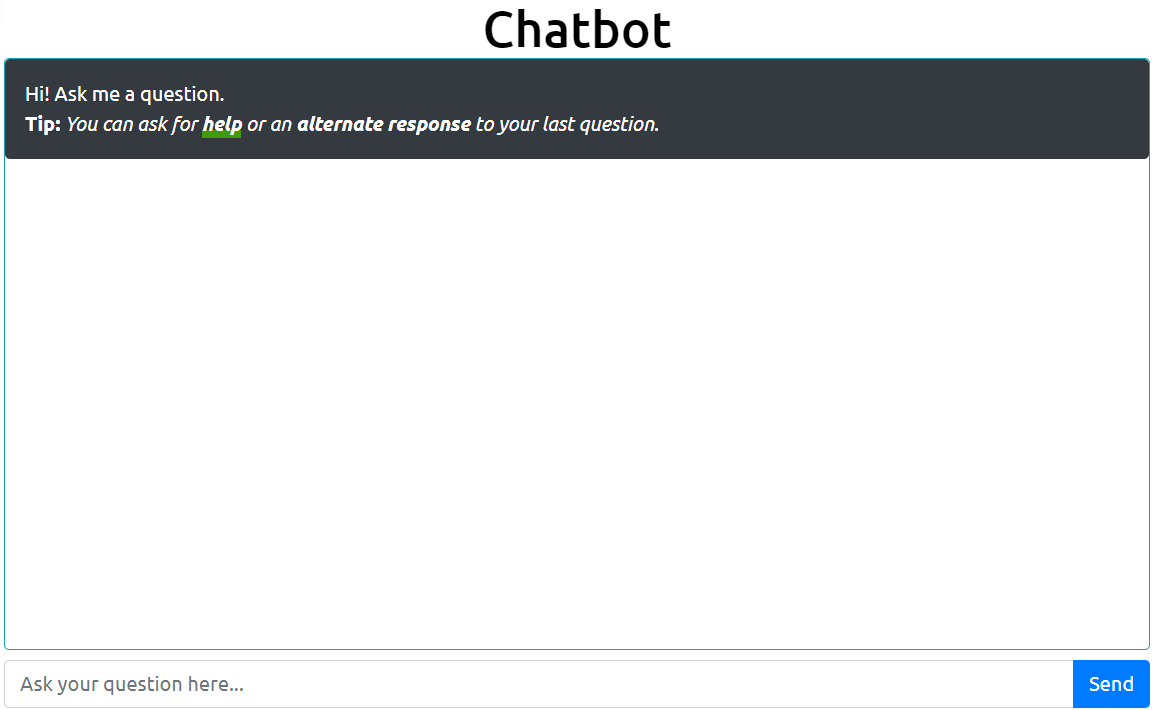
\includegraphics[width=1.0\columnwidth]{app-interface}%
    \caption{\captionstyle{The interface of the website.}}%
    \label{fig:site-interface}%
\end{figure}


\begin{lstlisting}[caption={\captionstyle{Using a variable passed from Python in a Jinja template.}}, label={lst:jinjavar}]

    <h1>{{ title }}</h1>

\end{lstlisting}

Aanother template, \texttt{chatbot.html}, implements the elements specific to the chatbot page: the chatbox, the text input field and the \enquote{Submit} button. It extends the \texttt{base.html} template. As a result, the elements defined in the base template are shown when the chatbot template is rendered and any additional elements can be inserted by defining a Jinja \texttt{block}.

\myparagraph{Styling}
The styling of the website was achieved with CSS. The CSS framework \textit{Bootstrap 4} by Twitter was used to style the website and to ensure that it can be viewed on devices with different screen sizes with no issues.

Although Bootstrap does not require any specific setup or configuration, the Flask extension Bootstrap-Flask can be used to implement a bootstrap layout more easily. It creates Jinja macros such as \texttt{bootstrap.load\_css()}, \texttt{bootstrap.load\_js()} which automatically load the required stylesheets and JavaScript which Bootstrap uses.

The chatbot page consists of three rows with one column per row. The title is positioned at the top of the page and the text input box and the button are positioned at the bottom. The chatbox is in the center of the page and it occupies all the remaining free space. By default, Bootstrap uses rows with the same height. However, custom css was written to position the elements more precisely and to change their height. To ensure the responsive design still worked, appropriate CSS size units such as \enquote{\texttt{\%}} and \enquote{\texttt{vh}} (viewport height) were used. The reason for this was that specific sizes, e.g. "20 pixels" are constant regardless of the screen size.

\subsubsection{Client-side Template Rendering}
Most instant messaging websites do not refresh their webpage when a message is sent or received. However, when implementing the input functionality, it was discovered, Flask does not provide a mechanism for dynamic manipulation of a website's content. Instead, templates are rendered to HTML once when the user accesses a page. To achieve dynamic message sending, JavaScript had to be used.

\textit{JavaScript} is a client-side programming language which runs inside web browsers. It can be used to dynamically change a website's content, store information and handle requests and responses. The JQuery library was used as it provides wrappers around JavaScript functions which allow for writing of less code to achieve the same functionality. It is already included in the HTML file as it is required by Bootstrap, so it could be taken advantage of its functionality.

This cannot be achieved with Flask since the page would have to be reloaded every time a message has been sent. Flask does not provide a mechanism for dynamically changing a website. However, this would introduce several problems such as loss of data when the page is reloaded and worse overall user experience. Additionally, the website would feel less responsive and slower. For these reasons the, JQuery DOM manipulation functionality was used. 

Whenever a message is added to the chatbox (a user or a bot message), a piece of HTML code is added to the current content of the chatbox. \cref{lst:msghtml} shows the HTML code for creating a message by the bot. On line 1, a div is defined. Its class value tells Bootstrap how to style the div: the background colour is set to dark grey, the text colour is set to white and rounded corners are used for the background. The code for creating a user message is the same, except for the background colour. Every time the user inputs text or the bot answers an input, this code is added to the HTML of the chatbox.

\begin{lstlisting}[language=HTML, caption={\captionstyle{The HTML code used to create a chatbox message sent by the chatbot.}}, label={lst:msghtml}]
<div class="p-3 mb-2 bg-dark text-white rounded">
I'm fine, thank you.
</div>
\end{lstlisting}

The first attempt of implementing this functionality used constant JavaScript strings which contained the necessary HTML code. The changing content, the message being added to the chatbox and the background colour, could be changed by appending several variables to the contents of the string. However, this turned out to be confusing, difficult to the debug and maintain. It was soon realised that it could be implemented using templates. Jinja templates seemed to be suitable for the task, however it was realised that Jinja could not be used in this case. Since the templates are rendered in the back-end when the user accesses the page, the templates could not be modified dynamically once the page is loaded. The reason for this is that Jinja is running on the server (the back-end), while JavaScript runs on the client (the user’s browser).

After researching the possible solutions to the problem, it was discovered that there exist templating engines for JavaScript. They provide the same functionality as Jinja, however they work on the client-side after the page is rendered. One such library is JsRender. It was ultimately selected due to its simplicity and speed of rendering templates as well as its syntax being very similar to Jinja. 

The code which would be reused had to be defined in one of the existing HTML files. It would have been preferable to store the templates in their own files as it would have provided better structure and separation of code. However, it was not possible as JsRender only supports such functionality on node.js servers. Instead, the templates were stored in the \texttt{chatbot.html} file. A requirement of JsRender is that templates are stored in an HTML \texttt{<script>} tag. The code for the message template can be seen in \cref{lst:jsrendertmpl}. 

\begin{lstlisting}[language=HTML, caption={\captionstyle{The code for the JsRender message template.}}, label={lst:jsrendertmpl}]
<script id="messageTmpl" type="text/x-jsrender">
<div class="p-3 mb-2 bg-<%:bg_col%> text-white rounded">
<%:text%>
</div>
</script>
\end{lstlisting}

On line 1, the template is defined. It can be referenced by the “id” value it is set. The value for \texttt{type}, \texttt{text/x-jsrender}, helps the library identify templates. Since this is not a standard script type (e.g. \texttt{text/javascript}), it is not rendered by browsers as they ignore types they do not know by default. On line 2, the HTML \texttt{<div>} with required class values is defined. Where normally the background colour of the div would be set, a JsRender variable is used. A colon before the name of the variable is used to signify that it is a JsRender variable. Its value is passed to the template from the Javascript code and is automatically replaced when the template is rendered. On line 3, using the same principle, a \texttt{text} variable is displayed. The standard tags used by JsRender are \verb|{{| and \verb|}}|. They are used to identify JsRender code. However they clash with Jinja’s tags and cannot be used as errors occur in Flask. Fortunately, JsRender provides a function to change the tags used. The tags were changed to \texttt{<\%} and \texttt{\%>} 

The templates defined in \texttt{chatbot.html} are rendered and used in the JavaScript program. \cref{lst:jsrenderrender} shows an example of rendering the message template. Since two variables are used in the template, \texttt{title} and \texttt{bg\_col}, they have to be passed when rendering it. This is done by creating the JavaScript object called \texttt{data} on line 1. The message text is stored in it as well as the necessary background colour which is set depending on whether the user or the bot has sent the message. On line 6 the template is loaded. JsRender can be used as an extension to JQuery by default, which is why the global JQuery variable \texttt{\$} is available. The template is rendered on line 7. It is required that any data is passed during this step. The result is the rendered HTML with the variable values substituted. The result is stored in a variable. It can then be added to the chatbox using a JQuery selector. The \texttt{append()} function is called on the selector to add the resulting HTML to the chatbox. This method does not require reloading of the page and it changes the content dynamically. 

\begin{lstlisting}[language=JavaScript, caption={\captionstyle{Rendering the JsRender message template.}}, label={lst:jsrenderrender}]
const data = {
"text": text,
"bg_col": user ? "info" : "dark"
};

const messageTmpl = $.templates('#messageTmpl');
const messageHtml = messageTmpl.render(data);
\end{lstlisting}

JsRender is also used for the loading animation and the error messages shown to the user when they haven’t given the program any input. The loading animation is pre-rendered as it does not have any dynamic content. The error message template utilises a Bootstrap alert which provides a coloured box which can be dismissed by clicking an “X” button in its top right corner. 

\subsection{Back-end and Front-end Communication}
The communication between the front-end and the back-end is required as the user input has to be sent to the back-end program for processing.The resulting output has to be sent to the front-end. This communication was achieved with the JavaScript. 

\subsubsection{Requests}
The JavaScript program forwards user questions to the back-end. Using JQuery event handlers, it is waited for a click on the Send button or the Enter keyboard key to be pressed. When either of these events occurs, the text stored in the text input field valided and passed to another method. If the user hasn’t entered any text, they are shown an error message. After it has been confirmed the input is valid, a GET request is sent to the server (the back-end program). The data is sent in the JSON format. Example JSON data can be seen in \cref{lst:regularreq}. Data passing can occur in the background without affecting the responsiveness of the page since JavaScript supports asynchronous requests. To let the user know that the program is processing their input, a loading animation is displayed. When the request is completed and a response has been returned by the back-end program, the loading animation is hidden and the bot response is added to the chatbox.   

\begin{minipage}{\linewidth}
	\begin{lstlisting}[caption={\captionstyle{Example data sent to the back-end for processing in the JSON format.}}, label={lst:regularreq}]
	{
		"request_type": "regular",
		"message": "Hi, how are you?"
	}
	\end{lstlisting}
\end{minipage}

\subsection{Extra Features}
Three extra features were implemented to improve the functionality of the application. 

\subsubsection{Command line Interface}
During development and testing, certain repetitive tasks had to be done manually. For instance, to collect training data, the “crawler” Python script had to be run every time. Since it is a seprate program, it had to be run manually. If any of its parameters were changed, e.g. how many pages are crawled or how many threads are used, its code had to be modified. For this reason, a command line interface was implemented so that a central place exists from where repeated actions could be run. 

Flask provides an interface for implementing custom commands. All Flask commands start with “flask” followed by the command name. For example, the command to run the Flask server, which can be executed from a terminal, is “flask run”. Optional parameters can be set using parameter switches. An example is running the Flask server with multiple threads with the command “flask run --with-threads”. Flask implements this functionality with the Python module Click.

The custom commands implemented are:
\begin{itemize}
    \item \texttt{flask crawl} – runs the crawler Python script to collect data from Stack Overflow. Optional parameters are:
    \begin{itemize}
        \item \texttt{-t, --threads} – how many threads should be used when crawling.
        \item \texttt{-p, --pages} – how many pages should each thread crawl.
        \item \texttt{-v, --verbose} – prints detailed command line output of what is currently happening.
    \end{itemize}
    \item \texttt{flask train} – trains the chatbot with the training data collected with “flask crawl”.
    \item \texttt{flask clean} – deletes the training data collected with “flask crawl”. Optional parameters are:
    \begin{itemize}
        \item \texttt{-y, --yes} – automatically deletes the files without asking the user for confirmation.
    \end{itemize}
    \item \texttt{flask del\_db} – deletes the database file for the chatbot. Optional parameters are:
    \begin{itemize}
        \item \texttt{-y, --yes} – automatically deletes the database without asking the user for confirmation.
    \end{itemize}        
\end{itemize}

%These commands were implemented for easier setup and usage of the application.

\subsubsection{Alternate Responses}
Stack Overflow threads usually contain more than one answer to a question. Furthermore, in programming, usually there are multiple ways to achieve something depending on the situation. This is why the web crawler by default collects more than one answer to a question. However, when the user asks the chatbot a question, by default the most upvoted response is selected. There is no way to access the other collected data. For this reason, an extra feature was implemented to allow the user to request an alternate response in the event that the original response wasn’t satisfactory.

The initial idea for the feature was to add a button to each response. If the button is clicked, another response would be given to the user. However, it was decided that a simpler implementation might be better. Since the user can “talk” to the chatbot, simply asking it to provide an “alternate response” would make the experience of communicating with the chatbot more authentic. The user would feel like they are communication with another person.

Several approaches to implementing this feature existed, however ultimately it was decided that the default BestMatch logic adapter should be modified. Normally, the BestMatch adapter generates two lists of responses – the \textit{response list} and the \textit{alternate response list}. The response list is first checked, and if one of the responses in it has a confidence value greater than a previously set threshold, it is automatically accepted as the best answer. If none of the responses has a high value of confidence, the alternate response list is created using different response selection parameters. Since these lists are generated every time a question is asked, they can be stored on the server. Therefore, there is always a list of possible alternate responses to the last question the user asked. 

The logic adapter returns the first response in the response list (index 0 of the list) by default as the list is ordered by confidence. If an alternate response is requested, a response from the cached list can be returned. This is achieved by calling the \texttt{pop()} method on the list of cached responses. It returns the item stored at the index given as a parameter and removes it from the list. Therefore, by calling \texttt{pop(1)}, an alternate response will be acquired as long as there are items left in the list. It is also checked whether a result can be returned from this index. If not, a message is returned instead to inform the user.

The logic adapter runs on the server, however client-side code is also required. In the chatbot Javascript program, an additional function was added to handle alternate responses. Every time the user provides input, it is checked if it matches the phrase “alternate response”. If it does, the function \texttt{getAlternateResponse()} is called with the input. Otherwise, the input is forwarded to the default \texttt{getBotResponse()} function. The function which provides alternate response works similarly to the regular response function. The main difference is the request it sends to the back-end. Since the request asks the server to perform a different action, its body contains extra information. To distinguish it from regular response requests, the value of the \texttt{request\_type} variable is set to “alternate” (to signify that an “alternate” response is requested) as opposed to “regular” (which signifies a regular response). 

The back-end function which processes the requests was also extended. When a request of type “alternate” is received, a response is requested from the bot. However, instead of asking for a response of a specific question, the command “ALT\_RESPONSE” is set as the question.  The BestMatch logic adapter then checks whether the question it is asked starts with the command. If it does, then the process described above is carried out.

\subsubsection{Feedback}
During the testing process of the application, it was discovered that the default response to some questions was not always the best response.  For this reason, another feature was implemented: user feedback. It would allow the user to "rate" a response. Better answers would receive higher rating. Thus, whenever new users use the application, they would receive answers with the highest rating.

The first step to implementing this feature was adding a voting or rating functionality to the front-end. The initial idea was to implement a star-rating system where 5 stars would indicate that the answer was very good, and 1 star would indicate that it was not coherent. However, a simpler to use system was implemented. Each time the user receives a response from the chatbot, the bottom part of the message box would contain a question to the user: “Was this answer helpful?”. The user would then be able to click on a “Yes” or “No” button to give feedback on the appropriateness of the answer. 

Implementing the feedback feature in the front-end side of the program required the creation of another JsRender template. The template contains the HTML code for the question and the two buttons. The text and the buttons do not need to change dynamically; however, they need to be uniquely identifiable. This is necessary as when one of the buttons is pressed, the question it refers to has to be identified. To implement this functionality, the feedback panel was placed inside a Bootstrap \texttt{row}. Each of these rows was given a unique \texttt{id} in the format \texttt{row-id-<ID>}, where \texttt{<ID>} refers to a unique integer. The code used to create the template can be seen in \cref{lst:feedbacktmpl}. 

\begin{lstlisting}[language=html, caption={\captionstyle{The JsRender template used to generate HTML code for a feedback panel.}}, label={lst:feedbacktmpl}]
    <script id="feedbackTmpl" type="text/x-jsrender">
    <hr/>
    <div class="row row-id-<%:btn_id%>">
        ...
    </script>
    \end{lstlisting}

In the JavaScript code, when rendering the template, a value for the variable \texttt{btn\_id} is passed to the template. The value is a unique integer which is incremented every time a feedback template is rendered. The same variable is used to identify each of the buttons. Additionally, each button has an \texttt{onClick} HTML property. In it, a function defined in the JavaScript program is called: the \texttt{getFeedback()} function. It takes 2 parameters: the unique ID of the button that was clicked and a string. The second parameter contains “yes” for the “Yes” button and “no” for the “No” button.

When \texttt{getFeedback()} is called, it processes the data passed to it. The ID value is used to find information about the answer the user wishes to rate. For this reason, all answers given to the user have to be stored. This can be done on the server-side, however, since JavaScript is a client-side language, the server-side history would contain data about all the answers sent to all users using the website. If there are a lot of users, searching through this data would take a lot of time and resources. For this reason, the decision to store this data on the client-side was made. Every time the user asks a question, the received response is stored in a JavaScript array. Incidentally, the position of each answer in the array corresponds to the unique ID of each of the buttons. Thus, the \texttt{getFeedback()} function can easily find the response in the array of all responses by selecting the item at index ID of the array. A request can then be made to server. The request body contains the following information: the type of the request (set to “feedback”) so that the request can be identified, the rating the user gave to the question (+1 or -1) and the answer itself. 

When the server receives a request of type “feedback”, it extracts all the data from it. The data is then passed the \texttt{bot.py} script. A function checks whether the feedback is “yes” or “no”. If the value is “yes”, then the function in the storage adapter \texttt{update\_rating()} is called with a parameter of 1, if it’s “no”, then -1 is passed to the same function. In order to find the response in the database, the text of the response is passed to the same function. The database is then searched using an SQL query created with the SQLalchemy library. The query selects a statement from the “statements” table the text of which is the same as the text passed to the function. The rating value of the selected statement can then be updated. Lastly, the changes are committed to the database.

\subsection{Summary}
\cref{fig:requestflow} illustrates the process carried out when a request is received by the back-end program.

\begin{figure}[htb]
	\centering
	\def\svgscale{0.7}
	\def\svgwidth{\columnwidth}
	\input{images/requestflow.pdf_tex}
	\caption{\captionstyle{A summary of request processing in the back-end.}}
	\label{fig:requestflow}
\end{figure}


\clearpage
\section{Evaluation}
The aim of this project was to investigate whether chatbots can be utilised in education. To achieve this goal, a protoype of a chatbot was created. The requirements set before the development started were as follows:
\begin{itemize}
    \item The application should produce coherent output when given user input.
    \item The application should utilise Natural Language Processing techniques to “understand” user input.
    \item The application should utilise Natural Language Processing to compare user input to known data.
    \item The application should have a user-friendly user interface.
    \item The application should be able to learn and improve through its interactions with users.
    \item The application should be easily trainable with additional data whenever necessary.
    \item The application should be accessible from both mobile and desktop computing devices.
    \item Etc?
\end{itemize}

This section will evaluate the implemented prototype. Two approaches will be taken: it will be compared to similar applications and a group of users will test it and provide feedback.

\subsection{Preparation}\label{subsec:prep}
To prepare the application for testing, firstly data was collected. The crawler program described in \cref{subsub:crawler} was used with the parameters summarised in \cref{tbl:crawlerparams}. To speed up the collection process, 4 threads were utilised. Each thread was assigned the task of crawling 10 pages of questions. The resulting data contained information about 600 questions. For each question, the 3 top answers were collected (where applicable, questions may have less answers). The resulting data contained approximately 1800 answers to 600 questions.

\begin{table}[!htb]
    \centering
    \renewcommand\arraystretch{1.6}
    \caption{\captionstyle{Parameters used for the web crawler when collecting data in preparation for testing.}}
    \label{tbl:crawlerparams}
    \begin{tabularx}{\textwidth}{XY}
        \toprule
        \textbf{Parameter} & \textbf{Value}  \\
        \midrule
        Number of threads & 4 \\
        Number of pages crawled by each thread & 10 \\
        Number of questions per page & 15\\
        Number of answers per question & 3 \\
        \hline
        Total questions collected & 600 \\
        Total answers collected & 1800 \\
        \bottomrule
    \end{tabularx}
\end{table}%

Even though it would have been beneficial to collect more data, Stack Overflow limit their incoming traffic. If a user sends too many requests to their servers, their access to the website is blocked. This proved to be a limitation in the data collection stage of the evaluation process. For this reason, the collected data was deemed satisfactory for testing purposes.

Secondly, the chatbot was trained using this data. In addition, the Python module "chatterbot-corpus" was also used for training. It provides example conversational data. In this case the data labelled "greetings" was used so that the chatbot can greet the user when input similar to "hi" and "how are you?" is provided. Chatterbot-corpus includes several other datasets, e.g. "jokes" and "trivia". However, these were not used as the purpose of this chatbot is to answer specific programming questions.

\subsection{Comparison with Cleverbot}
Cleverbot \citep{Cleverbot:online} is one of the most popular chatbots which currently exist. It was developed by Rollo Carpenter as a successor to the Jabberwacky chatbot. It was initially created in 1988 and was made public in 2006. It does not use machine learning to improve itself. Instead, a pattern matching technique is used to compare user input “fuzzily” to stored data from past conversations \citep{Cleverbot:online}. 

%In this regard, it can be said that it “learns” from its past conversations. Cleverbot utilises over 279 million past interactions which is about 3-4\% of the total data it has accumulated. Since it can use so much data when generating responses, it is expected that it will perform better than the chatbot developed for this project. Its data is much less in comparison due to lack of resources, time and users...


\myparagraph{Input correction}
Whenever Cleverbot is given user input, it corrects the punctuation and the word case if necessary. For instance, input such as “hi how are you” is converted to “Hi how are you.”. Commas and other punctuation marks will not be automatically inserted. It is also assumed that a full-stop should be added to the end of the sentence if it’s missing. The reason for this functionality is probably to allow Cleverbot to match the input to the data it uses to generate a response. 

While this approach might be beneficial, it does not work for the application developed for this project. A similar feature was tested by adding the JavaScript library Typopo. It can check text for common mistakes such as extra whitespace, extra dashes, wrong word case, etc. and correct it. The result, however, was not satisfactory. In programming, a lot of combinations of symbols are used which might be considered wrong by a spell-checking program. For instance, the question \enquote{what is the \texttt{-->} operator used for} is corrected automatically to \enquote{What is the \texttt{->} operator used for}. The library matches the input to known patterns, in this case the two dashes, and it removes one of them. This, however, changes the question asked by the user. If a \enquote{\texttt{->}} operator existed, a response related to it will be returned. Ultimately, this input correction functionality was not implemented. Furthermore, it is not required since punctuation and letter case do not affect the generated response since the chatbot does not utilise pattern matching.

\myparagraph{Context}
Cleverbot can have longer conversations with a user. For intance, consider the following conversation:

\begin{verbatim}
User: Tell me a joke.
Cleverbot: Knock Knock.
User: Who is there?
Cleverbot: Broken pencil.
User: Broken pencil who?
Cleverbot: Never mind it's pointless.
\end{verbatim}

The user asks for a joke and Cleverbot replies with the beginning of a “knock, knock” joke. The user then asks the bot for the rest of the joke twice and Cleverbot responds accordingly. To ensure that this is not random output of a statement, the joke was found online. Another version of the joke is as follows:

\begin{verbatim}
A: Knock, knock!
B: Who’s there?
A: Broken pencil.
B: Broken pencil who?
A: Forget it - this joke is pointless. 
\end{verbatim}

Through this interaction, Cleverbot appears to understand the context of the conversation. It is able to continue talking about a previously set topic. However, it is assumed that this possible due do the large amount of data Cleverbot has access to. A similar conversation with another user probably took place in the past and the user provided similar input to the bot’s statements. It is confirmed that Cleverbot has no knowledge of context by continuing the conversation:

\begin{verbatim}
[...]
Cleverbot: Never mind it's pointless.
User: Why is it pointless?
Cleverbot: Because I already know that.
User: What do you know?
Cleverbot: You're not too clever.
\end{verbatim}

In this case, the chatbot does not know how to continue the conversation and a response is selected from another conversation in its database.

On the other hand, the application developed for this project neither has any knowledge of context nor tries to imitate it. For instance, when asked the question \enquote{what are move semantics?}, the bot replies successfully. However, if the user tried to continue the conversation by asking “when to use them?” to bot is unable to generate a response. It should be noted that if it had data about a question similar to \enquote{when to use them?}, the response to that question will be returned to the user. Therefore, the chatbot is unable keep track of previous statements in the conversation. Such a feature would be extremely beneficial; however, implementing it would not be a trivial task and such a system with context awareness has yet to be created. A similar approach to Cleverbot could be taken where whole conversations are stored. However, Cleverbot is able to learn from conversations with its users since it does not have a specific domain of knowledge. On the other hand, this chatbot’s purpose is to teach students by giving them answers it already knows. For this reason, it would be unable to learn from user input. Additionally, because of this realisation, the chatbot was made \enquote{read-only} which does not allow it to store conversations with its users.

\myparagraph{Paraphrased input}
Cleverbot can answer the same question worded differently. For example, if the user asks “what is your favourite colour?”, Cleverbot replies “Don’t have one.”. If the user then asks “what colour do you like the most?”, the bot replies with “Blue.”. Even though the answers to both questions do not match, they are coherent and are linked to the question. However, this is probably possible due to the amount of data Cleverbot has access to. Nevertheless, Cleverbot can process paraphrased user input. 

On the other hand, the chatbot developed for this project cannot respond to paraphrased input. For example, when asked “how are you?”, it replies with “Very well, thanks”. If the question is changed to “how is it going?”, it responds with “Good.”. This is possible because the chatbot database contains responses for both questions. In reality, the chatbot is not necessarily able to realise both questions have very similar meaning. Furthermore, when asked “what is the difference between a pointer and a reference?”, the chatbot generates a correct answer. Analysing the training data shows that the statement the chatbot “knows” is actually “What are the differences between a pointer variable and a reference variable in \texttt{C++}?”. Therefore, it is able to process partially paraphrased input. However, it should be noted that most of the words which convey the meaning of the sentence are present in the paraphrased question. Thus, it should not be surprising that the results are good. Unfortunately, when the question is paraphrased drastically to, for instance, “references vs. pointers”, the chatbot replies with a known reply to the statement “When to use references vs. pointers”. While the information might be useful for the user, their intention was to find out is the differences between the two are, not when to use each one.

Unfortunately, no easy solution to this problem exists. Making the bot “smarter” would require developing a more complex system. Furthermore, using a premade library would be impossible. Instead, the system would have to be written for this specific purpose. However, a suggestion for improvement of this chatbot is given: after the training data is collected, another program could read each question, and generate paraphrased questions from it. The answers of the original questions can then also be associated with the paraphrased versions. This would be a naïve solution, however it might produce satisfactory results for the purposes of this project.

\subsection{User Testing}
A group of users was asked to provide feedback for the application twice. The first time was after completing the initial prototype of the website described in \cref{sec:impl}. Four users were asked to test the application and provide general feedback. The aim was to find out whether the application was user-friendly and worked as expected. The second testing session was after some changes were implemented based on the feedback from the first session. A larger number of users were asked to participate.

\subsubsection{First Testing Session}
The first testing session took place after an initial prototype of the application was built. All features described in \cref{sec:impl} were implemented and could be used. Five users participated in the session. All of them were Computing students in their final year at university. All of them had advanced overall knowledge of programming and at least intermediate knowledge of \texttt{C++}. The aim of this session was to identify user interface problems so that the application can be made more user-friendly. Additionally, another objective was to find bugs in back-end or the front-end. The users were not asked any specific questions and were able to provide feedback in the form of notes without any specific format.

\cref{app:sesh1} illustrates the result of the first testing session. The column named "Feedback" lists the points the testers made about what they thought should be changed. The column "Changes made" describes what changes were implemented based on the user feedback. It should be noted that the results table only shows the negative feedback received. A more detailed summary of the problems and their solutions follows.

All testers agreed that the style of hyperlinks was not satisfactory. One of the testers made the point that it looked like a "grammatical or spelling error which is underlined by a spell-checking program". This is caused by the initial style that was implemented: the text colour of hyperlinks was white (the same as regular text), and they were underlined with a red line. Changing the colour to yellow and green was tested, however, the same tester noted that it still looked like a "grammatical error" due to these colours being associated with errors (red), warnings (yellow) or correctness (green). Another tester suggested using a different colour for the hyperlink text and underlining it with a line of the same colour. In the end, this idea was implemented, and the colour of hyperlink text and underlining was changed to light blue. As a result, the testers agreed that it looked better and it was clear which words were a hyperlink. 

Another problem caused by the style of hyperlinks was that the "help" link in the initial chatbot message was not visible. The testers thought it was emphasized but did not realise they can click it. Additionally, they did not realise they can use the "help" command by typing "help" as a message in the chat. This was caused by their inability to access the help message which could only be seen by clicking on the "help" link. To rectify this problem, an additional "help" button was added at the top of the page. Furthermore, the initial chatbot message was changed to specifically tell the user they can either type "help" in the chat, click the "help" link or click the button at the top of the page. As a result, the testers agreed that this is more user-friendly.

One tester made the point that typing the "alternate response" command can become tedious when it is done repeatedly. They suggested adding a button. The button was added to the bottom of every bot message (in the panel for feedback). After testing the changes, the testers agreed that while this solution worked, the button was only accessible if the user hasn't clicked on the feedback buttons. If one of them is clicked, the contents of the panel change. A suggestion to add the button to the message shown when the user clicks the "no" feedback button was made. Since clicking the "no" button means that the user was not satisfied with the response, it would make sense to add the "alternate response" button to the new message shown. This change was also implemented, and the testers agreed that the result was satisfactory.

One of the users who tested the website on a desktop computer with a large screen noted that the webpage fills their entire browser window. While this is to be expected as the responsive design of the website ensures that the content's size adapts based on the screen, this caused a problem. The tester said that this makes it very difficult to read long answers as they look like a “wall of text”. After researching what other websites with a lot of text do to fix this problem, it was realised that very rarely websites use the full width of the screen. Usually, columns on the left and right are used for other content. The text takes up about 60\% of the width of the screen. Additionally, while online chatrooms often used the full width of the browser window, the text messages rarely take up that much space. As a result, the width of the Bootstrap Container was reduced. This change only affected devices with big screens. No changes were made for mobile devices. The testers agreed that it was easier to read longer responses.

Other smaller changes made based on the feedback were:
\begin{itemize}
    \item The help message was changed to more clearly indicate what features the user has access to and how to use them.
    \item Another webpage (\enquote{about this project}) was added to explain the purpose of the website and to give credit to Stack Overflow for the data collected from there.
    \item A navigation bar (menu) was added to the top of the page with a \enquote{Home} and \enquote{About} buttons which redirect to the respective pages. The \enquote{Help} button was also placed in the menu. Clicking on it, simply writes \enquote{help} as a question on behalf of the user. The testers agreed they liked this behaviour since it teaches the user how to use text commands. For this reason, the functionality was kept.
    \item One of the testers discovered that while waiting for a response, more questions can be asked which results in the inability of the bot to respond. To fix this problem, the \enquote{Send} button was disabled while waiting for a response as well as pressing the \enquote{Enter} keyboard key. 
\end{itemize}

Lastly, the testers agreed that the bot was able to respond to about half of their questions. However, this was to be expected since the training data used was of limited quantity.

The improved website can be seen in \cref{fig:newui}.

\begin{figure}[!htb]%
    \centering
    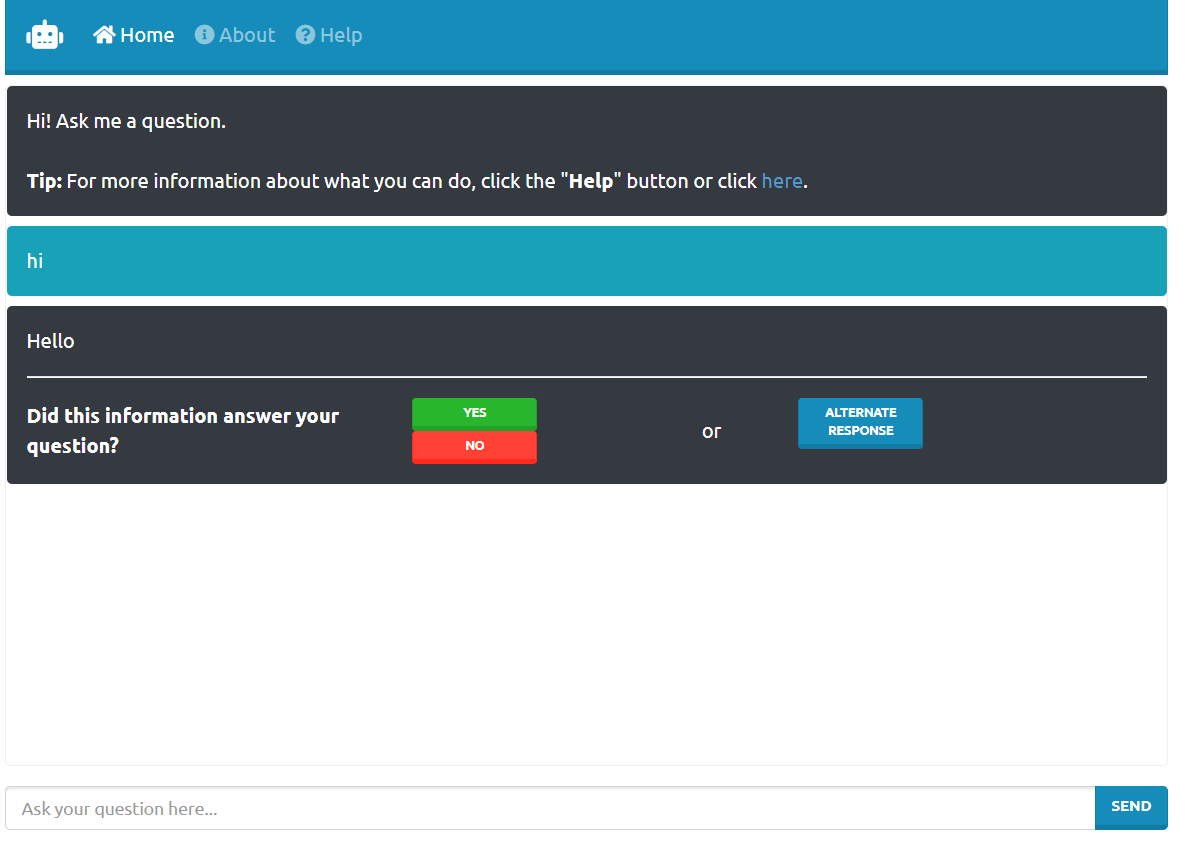
\includegraphics[width=1\columnwidth]{newinterface}%
    \caption{\captionstyle{The improved user interface.}}%
    \label{fig:newui}%
\end{figure}

\subsubsection{Second Testing Session}
% $\sfrac{3}{4}$
%\cref{fig:progknowl,,fig:ui} <- change second one
For the second testing session, the same data collected in \cref{subsec:prep} was used. A second website was hosted on PythonaAnywhere so that the users can access it from their own devices. The development branch of the repository was hosted as it was unclear whether the changes made after the first testing session could be considered stable.

The aim of the session was to test the improved prototype with as many users as possible. In the first testing session the participants had more advanced knowledge of programming. However, in the second session the objective was to have the application tested by beginner programmers. Since the target audience for the project is new university students, it was estimated that the results would be more accurate with this approach. 

For the testing session a questionnaire was prepared using the website SurveyGizmo. It was selected as it provided a free account plan which does not limit the questions per survey. The final questions can be seen in \cref{app:surveyqs}.

Each tester was sent a link to the survey and a link to the newly set up website. They were given a short description of the aim of the project, and were informed that the chatbot can answer specific \texttt{C++} questions. Each participant was also instructed to test the application and then complete the survey. Twelve testers agreed to take part.

\myparagraph{Results}
A bar chart of the responses to question 1 can be seen in \cref{fig:progknowl}. The results showed that 50\% of the participants were beginner programmers. This is result is satisfactory as feedback from users with different knowledge levels will be available while most of them are new programmers. 

\begin{figure}[!htb]%
	\centering
	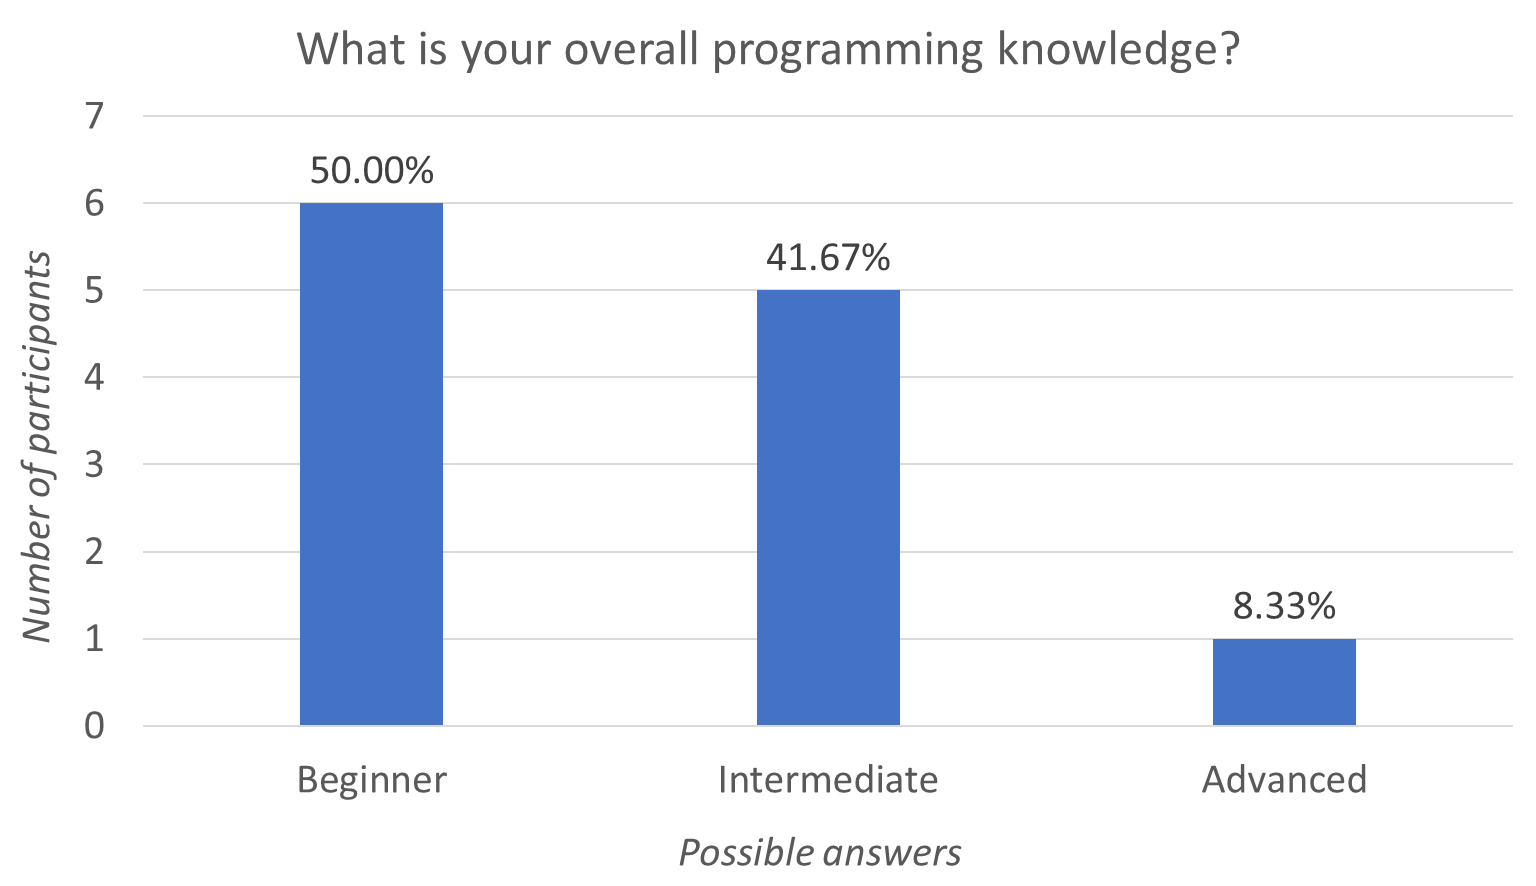
\includegraphics[width=1\columnwidth]{q1}%
	\caption[Bar chart showing the overall programming knowledge level of the participants in the survey.]{\captionstyle{Bar chart showing the overall programming knowledge level of the participants in the survey. The y-axis corresponds to the number of participants who selected an answer, while the x-axis represents each possible answer.}}%
	\label{fig:progknowl}%
\end{figure}


The results for question 2 can be seen in \cref{fig:ui}, The results were positive, and they proved that the changes made after the first testing session were favourable.

\begin{figure}[!htb]%
	\centering
	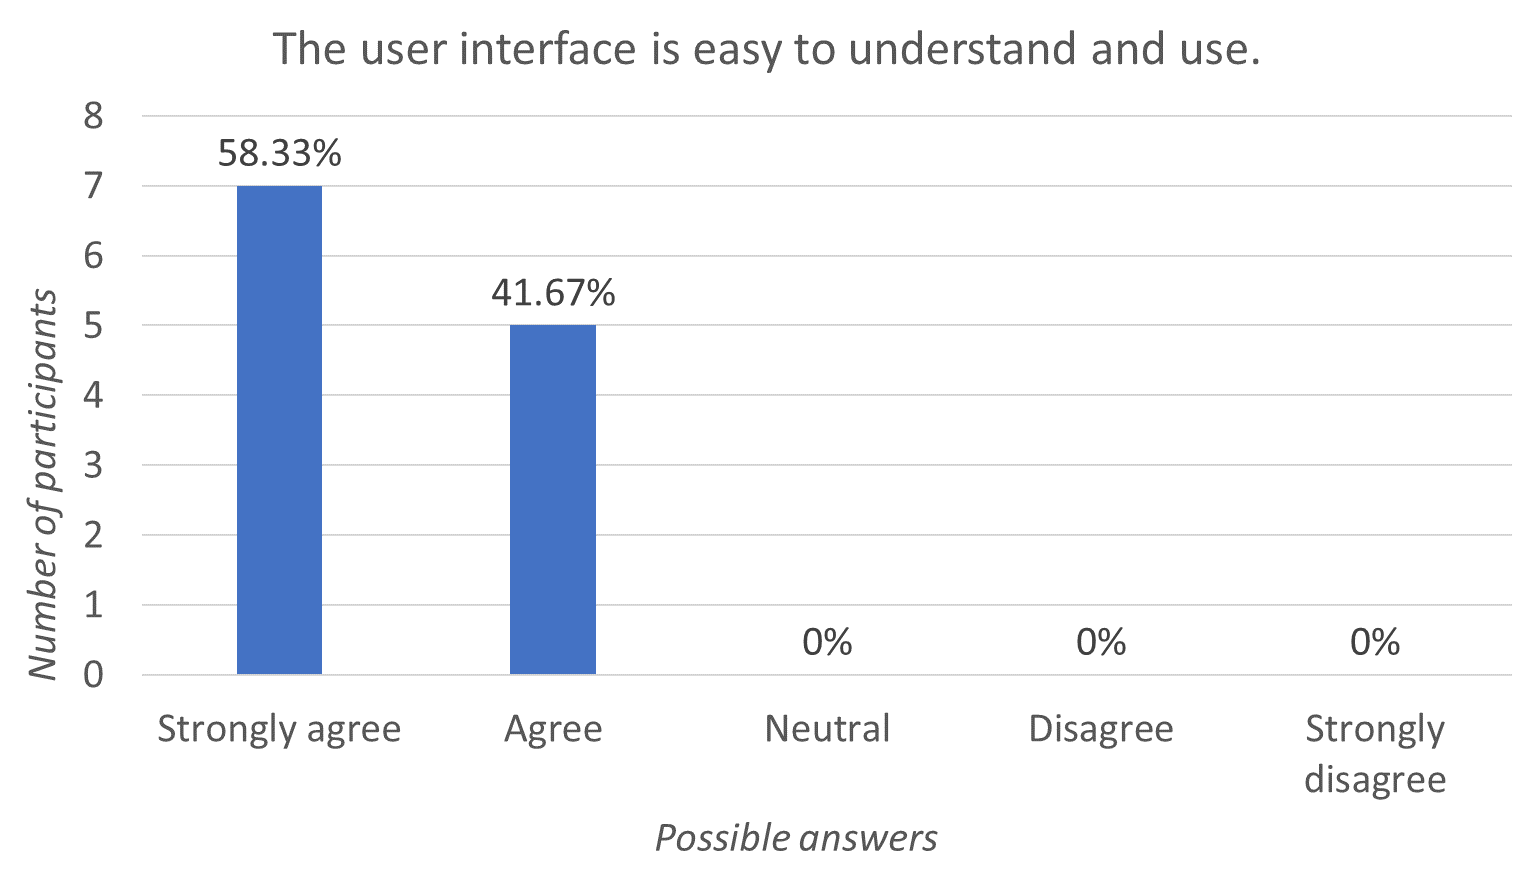
\includegraphics[width=1\columnwidth]{q2}%
	\caption[Bar chart showing the responses to question 2.]{\captionstyle{Bar chart showing the responses to question 2. The y-axis corresponds to the number of participants who selected an answer, while the x-axis represents each possible answer.}}%
	\label{fig:ui}%
\end{figure}

Questions 5 asked the users if they were able to use the alternate response feature. The results show that 16.67\% answered that they neither agree nor disagree and 8.33\% that they disagree. When asked what prevented them from using the feature, their feedback was that whenever the chatbot answered with an incorrect response, the answer produced by the alternate response feature would be an answer to the same wrong question. This behaviour, however, is to be expected since the alternate response feature selects another response from the previously generated list of responses. To improve this feature, it would be required to regenerate the list of responses every time the user requests an alternate response instead of storing it the first time they ask a question. The results are illustrated in \cref{fig:altr}.

\begin{figure}[!htb]%
	\centering
	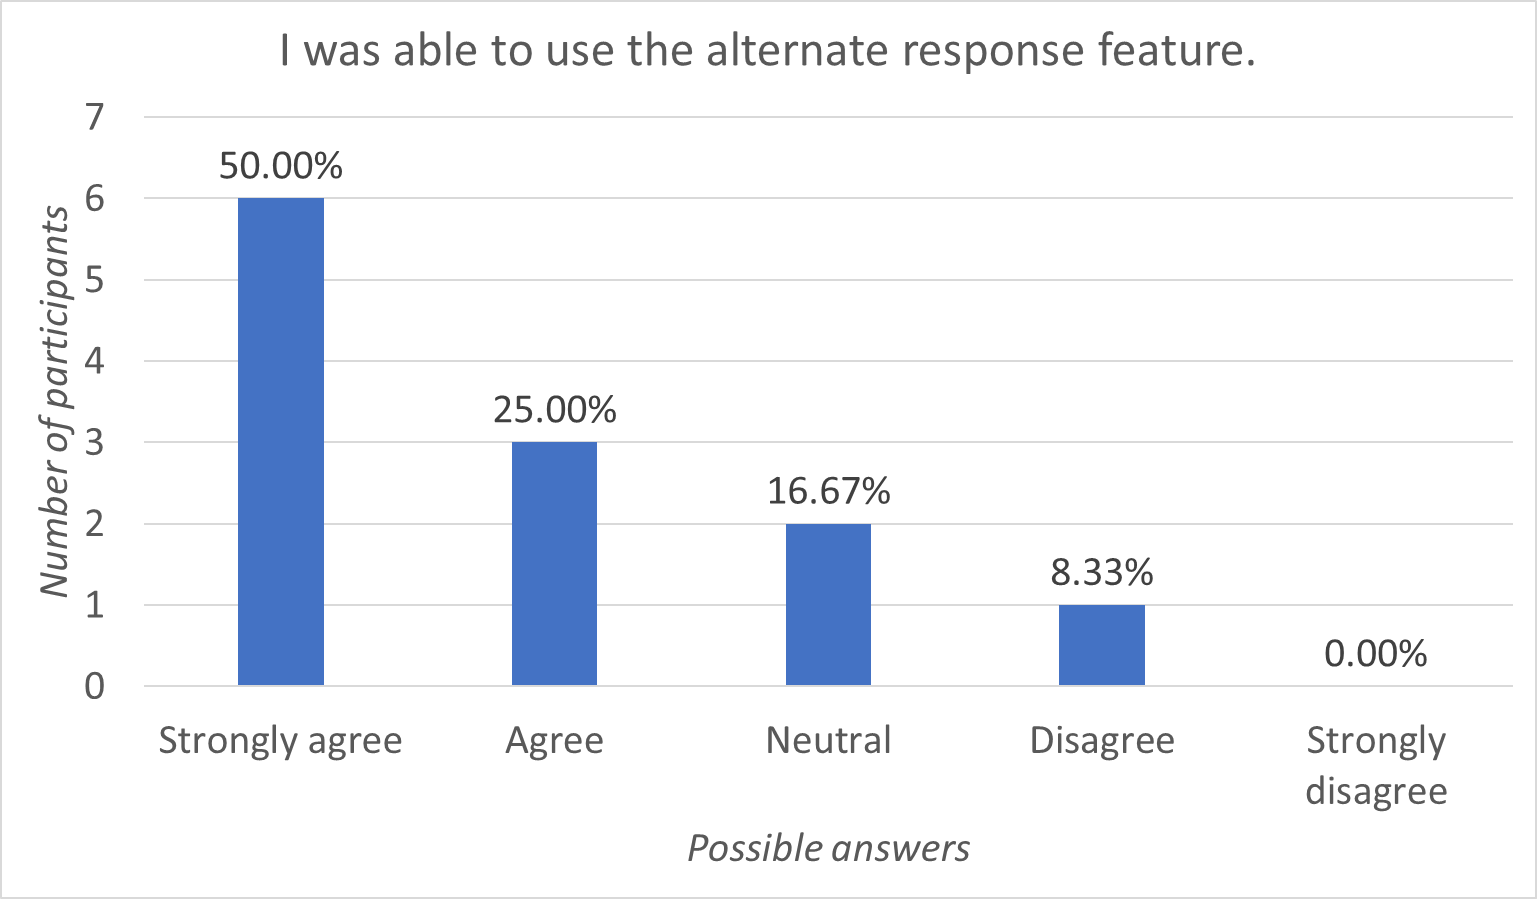
\includegraphics[width=1\columnwidth]{q5}%
	\caption[Bar chart showing the responses to question 5.]{\captionstyle{Bar chart showing the responses to question 5. The y-axis corresponds to the number of participants who selected an answer, while the x-axis represents each possible answer.}}%
	\label{fig:altr}%
\end{figure}

The results for question 6 show that 8.33\% neither agreed nor disagreed. When asked why the selected this answer, they replied that they did not understand how this feature affected the future responses of the chatbot. For this reason, a consideration was made to add an explanation in the help message since it would motivate the users to use the feature. As a result, the chatbot will improve more. The results for this question can be seen in \cref{fig:fdbk}.

\begin{figure}[!htb]%
	\centering
	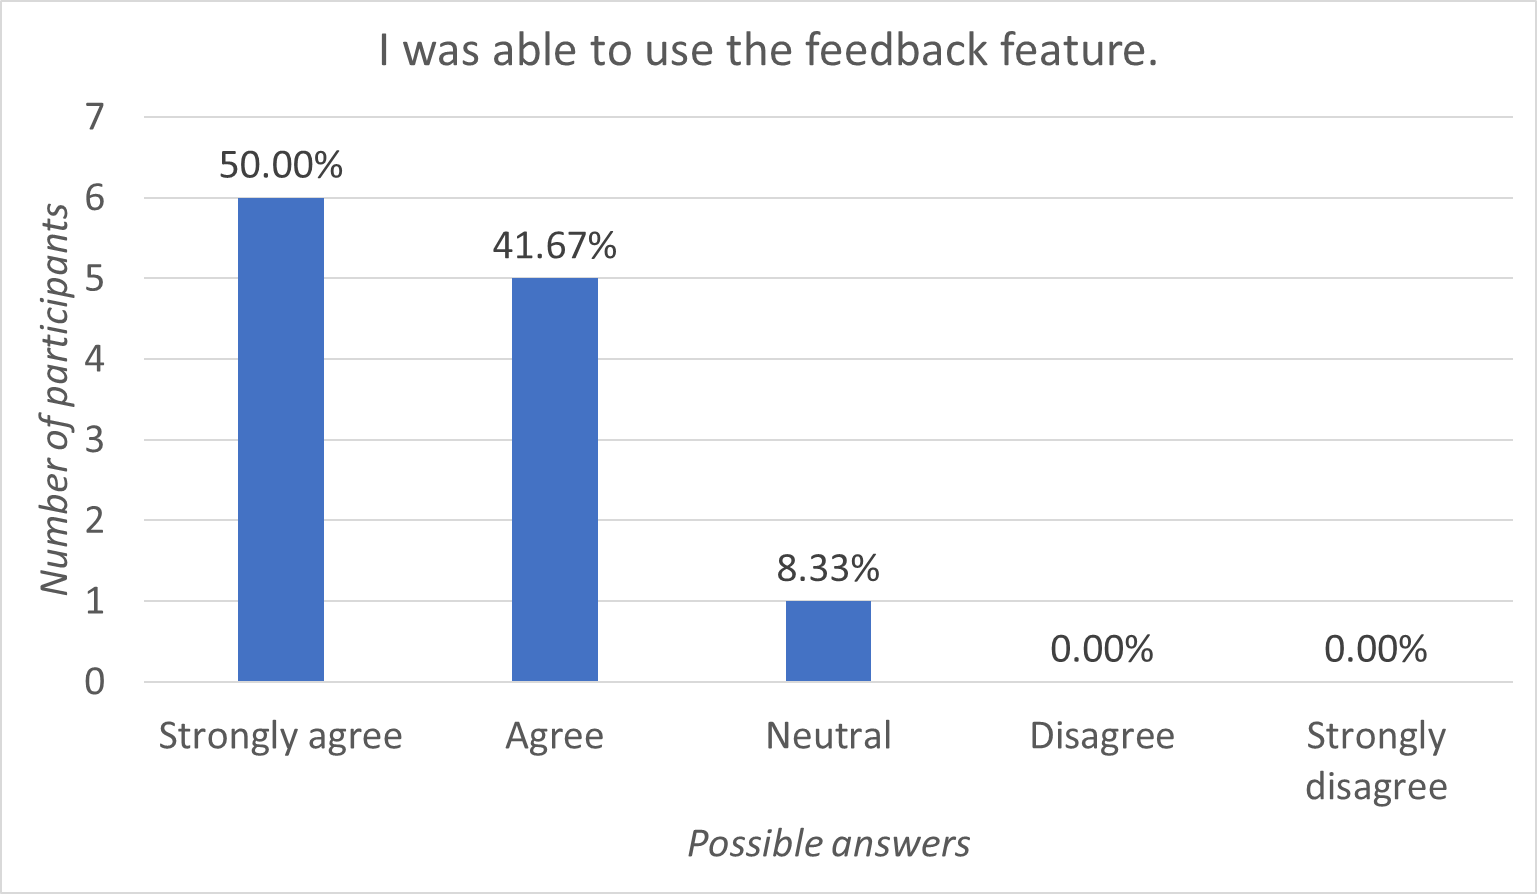
\includegraphics[width=1\columnwidth]{q6}%
	\caption[Bar chart showing the responses to question 6.]{\captionstyle{Bar chart showing the responses to question 6. The y-axis corresponds to the number of participants who selected an answer, while the x-axis represents each possible answer.}}%
	\label{fig:fdbk}%
\end{figure}

The answers for question 7 were positive (“appropriate error messages are shown”). The users responded that they strongly agree (58.33\%) and that they agree (41.67\%).

The results for question 8 were not considered as it was realised that the free hosting option on PythonAnywhere limits the speed of operation of the application. However, the results were positive probably due to the small amount of users using the website concurrently.

Question 9 asked the user whether the chatbot answered their questions accurately. 16.67\% answered that they neither agree nor disagree. When asked why they chose this answer, the participants said that the chatbot was unable to answer some of their questions. This was a result of the limited amount of training data. The answers to question 9 are summarised in \cref{fig:accurate}.

\begin{figure}[!htb]%
	\centering
	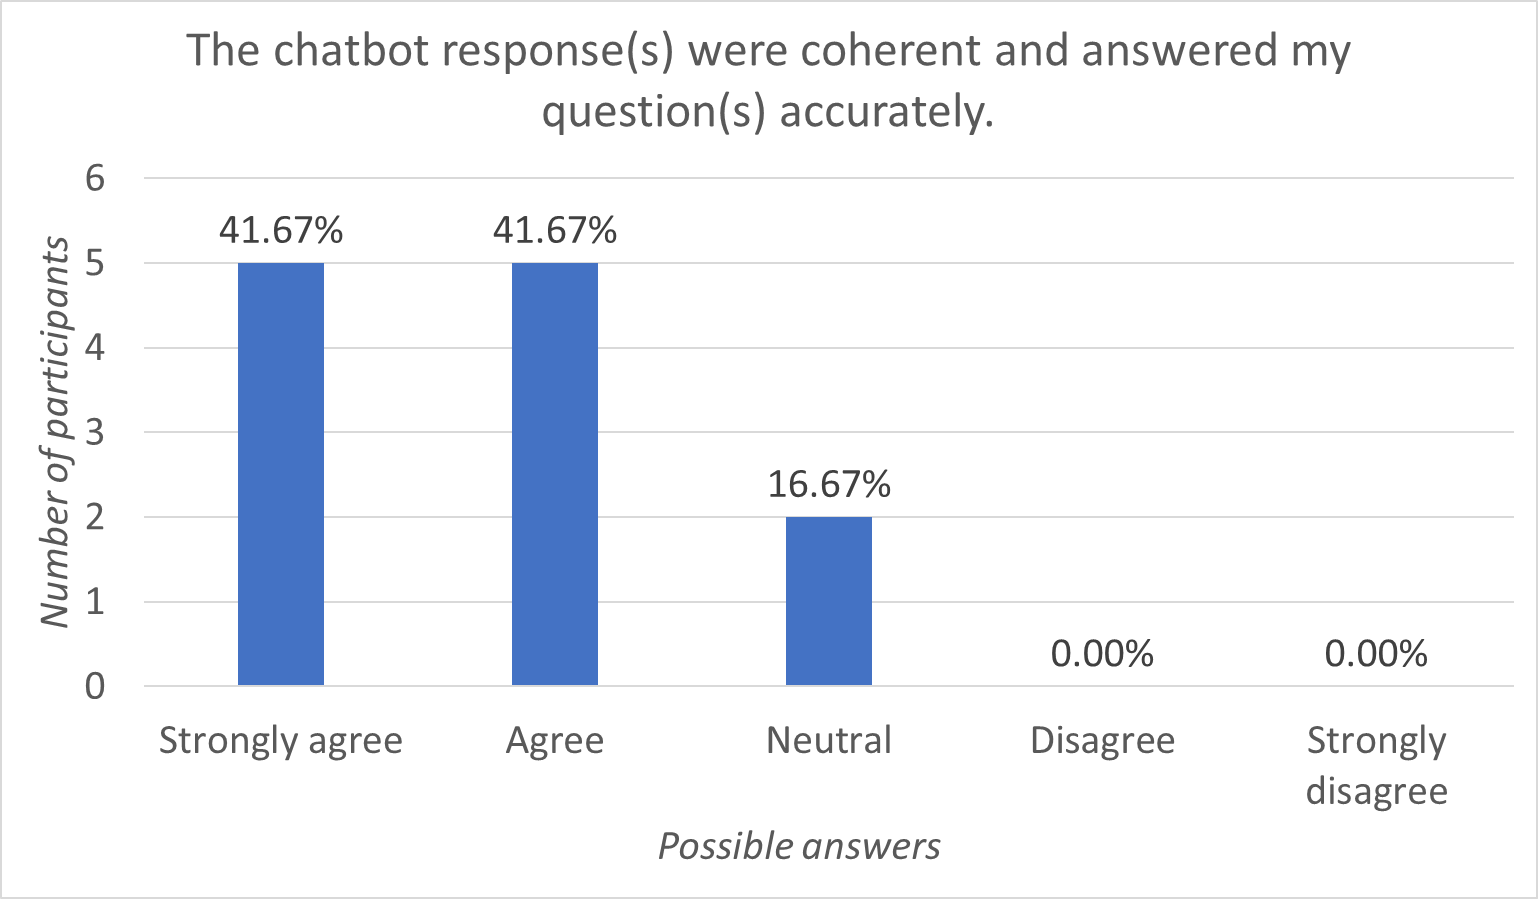
\includegraphics[width=1\columnwidth]{q9}%
	\caption[Bar chart showing the responses to question 9.]{\captionstyle{Bar chart showing the responses to question 9. The y-axis corresponds to the number of participants who selected an answer, while the x-axis represents each possible answer.}}%
	\label{fig:accurate}%
\end{figure}


The feedback for question 10 was positive: 66.67\% of the testers strongly agreed and 33.33\% agreed that they were overall satisfied with the application. As a conclusion, it can be said that the participants approved of the prototype since most of the responses were positive.

Most of the testers did not provide any additional feedback in the last question. One made the point that the layout of the website did not work on their smartphone (iPhone). The webpage did not fit in their browser window. Another piece of feedback was that the chatbot does not respond to questions which include symbols such as \texttt{\&, [, ], |}. However, when trying to find out what caused that problem, no issues were found with these symbols. Another tester mentioned that the chatbot could not respond to general questions such as “what is \texttt{C++}?” and “what is the difference between \texttt{C++} and other languages”. Even though the purpose of the chatbot was to help with specific problems, such questions are beneficial information for new programmers. Additional data was collected from the official website of the \texttt{C++} standard \citep{cppfaq:online} by creating another crawler program (see \cref{app:crawler}).

Lastly, one of the testers noticed that there was a problem with the feedback feature which only occurred for some responses. An example is sending the message “hello” to the bot. The initial response is “Hi”. When the feedback feature is used to downvote the answer, the bot chooses the next response (“Greetings!”). However, if this answer is voted negatively, the bot does not return the initial answer (“Hi”). It was discovered that this is caused by how the data is stored into the database. When updating the rating of the response, the search for an entry with text “Greetings” finds a result with an empty “in\_response\_to” value. This means this value is never selected from the database when the user asks a question. To fix this problem, an additional requirement was added when selecting an entry from the database: it is checked whether the “in\_response\_to” field is empty.

A summary of the feedback from the survey is presented in \cref{tbl:surveyresults}. The percentage of "strongly agree" responses was 57.4\% of the total responses. The users selected "agree" for 36.1\% of the responses, 4.6\% of the responses were "Neutral" and 1.9\% were "Disagree". It can be concluded that the feedback was very positive even though some issues were highlighted.

\renewcommand\arraystretch{1.8}
\begin{sidewaystable} %{addcode={\caption{Test}}, angle=-90}
	\caption{\captionstyle{A summary of the results from the questionnaire.}}\label{tbl:surveyresults}
	\begin{tabularx}{0.95\textheight}{Xccccc}
		\toprule
		Question & \tiny{\textbf{Strongly agree}} & \tiny{\textbf{Agree}} & \tiny{\textbf{Neutral}} & \small{\tiny{Disagree}} & \small{\tiny{Strongly disagree}} \\
		\midrule
		The user interface is easy to understand and use. & 7 & 5 & 0 & 0 & 0 \\
		The user interface is visually pleasing. & 6 & 5 & 0 & 1 & 0 \\
		I was able to understand how to use all the features of the application. & 8 & 4 & 0 & 0 & 0 \\
		I was able to use the \textbf{alternate response feature}. & 6 & 3 & 2 & 1 & 0\\
		I was able to use the \textbf{feedback feature}. &  6 & 5 & 1 & 0 & 0\\
		Appropriate error messages are shown. & 7 & 5 & 0 & 0 & 0 \\
		The chatbot answered my question(s) quickly. & 9 & 3 & 0 & 0 & 0 \\
		The chatbot response(s) answered my question(s) accurately. & 5 & 5 & 2 & 0 & 0 \\
		I am overall satisfied with the functionality of the application. & 8 & 4 & 0 & 0 & 0 \\
		\hline
		\textbf{Total} & 62 & 39 & 5 & 2 & 0 \\
		\bottomrule
	\end{tabularx}
\end{sidewaystable}

Overall, it can be concluded that the testers were satisfied with the application. Since this is an initial prototype, problems could be expected, however some issues could have been avoided by simply collecting more training data.

%\begin{figure}[!htb]%
%    \centering
%    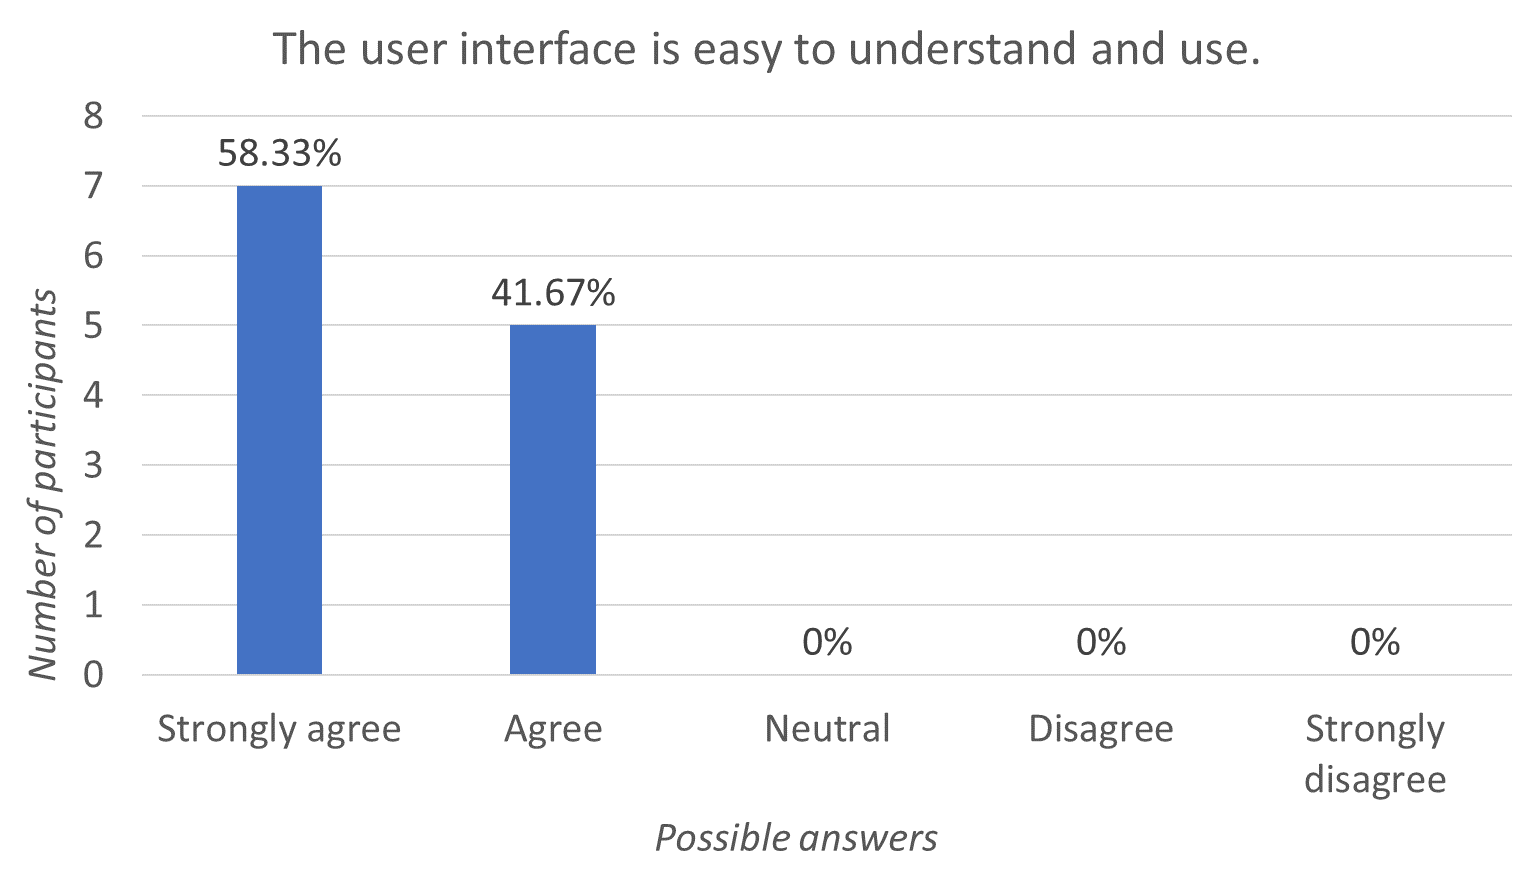
\includegraphics[width=1\columnwidth]{q2}%
%    \caption{\captionstyle{Bar chart showing the overall programming knowledge level of the participants in the survey.}}%
%    \label{fig:progknowl}%
%\end{figure}
%
%\begin{figure}[!htb]%
%    \centering
%    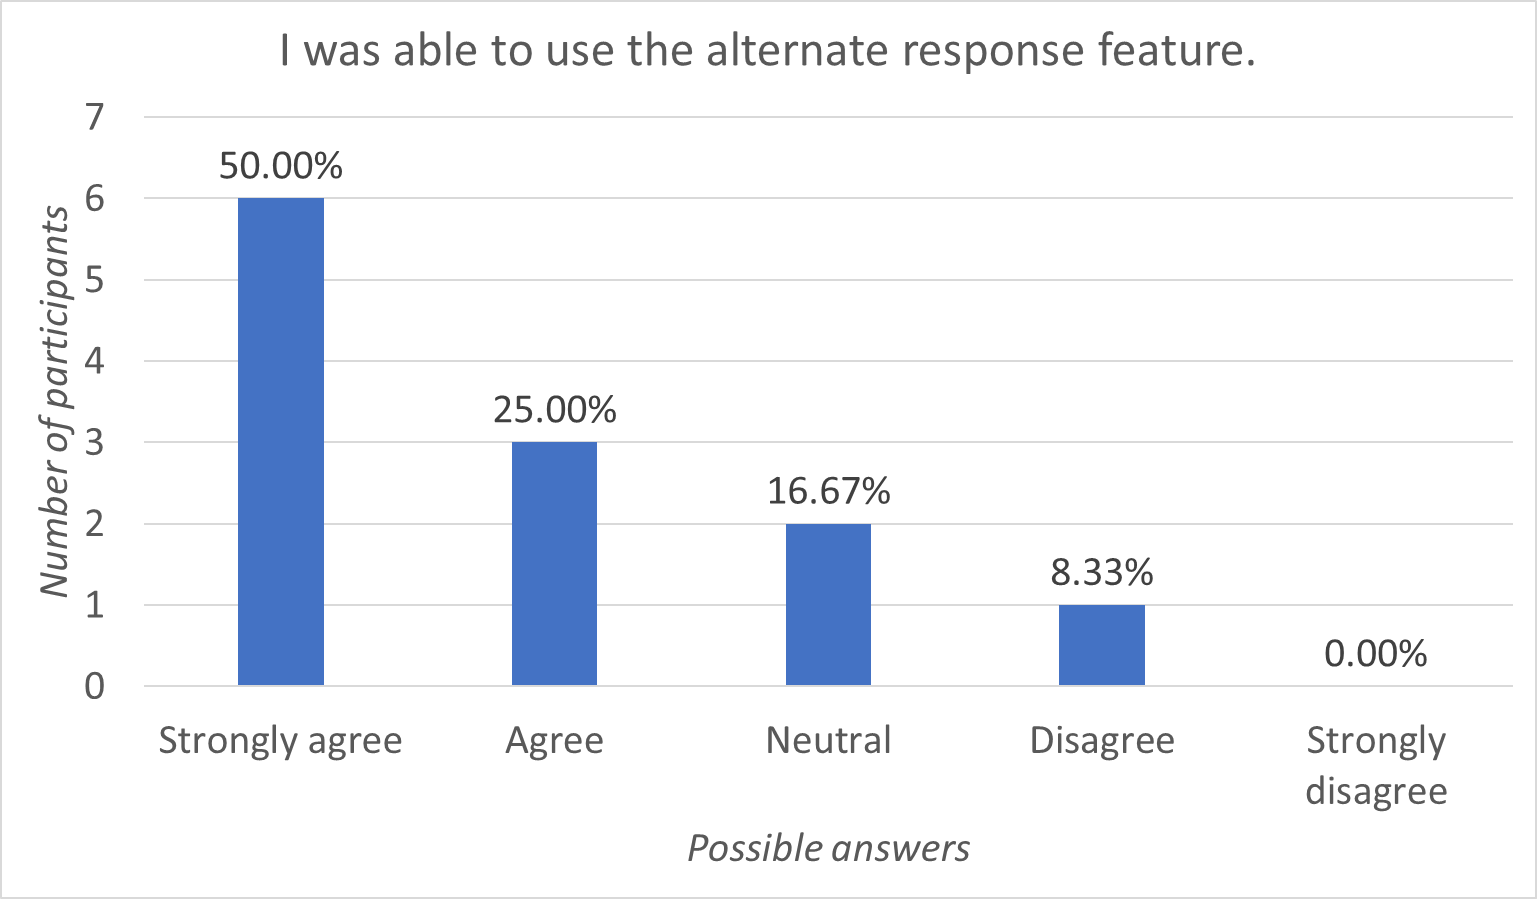
\includegraphics[width=1\columnwidth]{q5}%
%    \caption[Bar chart of the result of survey question 5.]{\captionstyle{Bar chart of the result of survey question 5 (\enquote{The user interface is easy to understand and use.}). The number of users who selected each response is along the y-axis. Each possible answer is along the x-axis.}}%
%    \label{fig:ui}%
%\end{figure}

\newpage
\section{Conclusions}
The aim of the project was to investigate whether chatbots can be used as a tool in education by implementing a suitable application and evaluating it.

A review of academic literature was conducted to highlight some of the key technologies and concepts related to the development of a natural language generation systems. In addition, similar existing applications were investigated so that the approaches to their devlopment could be compared. The results of the review were used during the development of a prototype of the proposed software.

The initial objectives of the project were met. A system which can successfully be trained with data about a desired topic was implemented. Furthermore, the system was made easily accessible since it provides an online interface which adapts to the screen size of the device used. The interface design decions made were based on existing messaging applications which have poven to be user-friendly. In addition, extra features were added which surpassed the initial plan. Lastly, the configuration process of the system was simplified so that an administrator could configure and use it easily.

The project was evaluated by comparison with a similar application. The results showed that the rivalling program was more advanced, however its superiority can be mostly attributed to the large amounts of training data it has access to, not the response selection method. Moreover, the system developed for this project was evaluated by a group of users which resembles its expected target audience. The results were overwhelmingly positive, even though issues were discovered. The participants were overall satisfied with the system.

The areas where the project did not meet its objectives were its ability understand natural language. While the deliverable utilises Natural Language Processing techniques to process input and generate output, the algorithm is limited. This is mainly due to the library selected for the implementation of the back-end. The chatbot can answer questions, however training data of high quality and large quantity would be required for more advanced use. There were factors which prevented the collection of more data in this study, however the web crawling program that was developed would be able to achieve this if there were no outside restrictions. Other issues highlighted by the testers were problems with the responsive design and the inability of the application to answer paraphrased questions.

To conclude, it  can be said that the delivered chatbot could find use. It would be impossible for it to provide as much knowledge as a teacher, however it can be used by a teacher to provide ready access factual data. 

\newpage
\section{Future Work}
While the project met most of its requirements, its functionality can be improved as the evaluation process showed. The following suggestions for improvements and additions are made:
\begin{itemize}
	\item The alternate response feature can only retrieve previously stored responses. While this approach works, if the chatbot failed to identify the question initially, the alternate responses returned would be incorrect as well. A solution  to this problem would be searching through the database and generating a new list of responses using different parameters when the user request an alternate response. This solution would be slower, however the responses would be more accurate.
	\item The chatbot should be able to understand paraphrased input. At present, it is able to do so in some cases. However, improving this system would be crucial since it would be able to respond to more questions and provide more assistance.
	\item The user interface is not compatible with some mobile devices as some of the testers discovered. It should be improved since it is expected that it will be used often. The participants of the survey also confirmed that they prefer using the application on a mobile device.
	\item An online retrieval feature could be added in the event that the chatbot does not have information about a question. It could perform a web search and display relevant URLs to the user.
	\item An administrator page could be added where the chatbot can be configured instead of using the command line interface. Furthermore, statistics could be displayed about the number of questions the chatbot has answered and an interface for adding more training data could be implemented.
\end{itemize}

\newpage
%\bibliography{./references}
%\bibliographystyle{apalike}
\printbibliography[
	heading=bibintoc,
	title={References}
]

%you can crate this on a extra tex document just like the title or any other part of the document.
\newpage
\begin{appendices}
\crefalias{section}{appsec}
\section{Project Overview}\label{app:ipo}
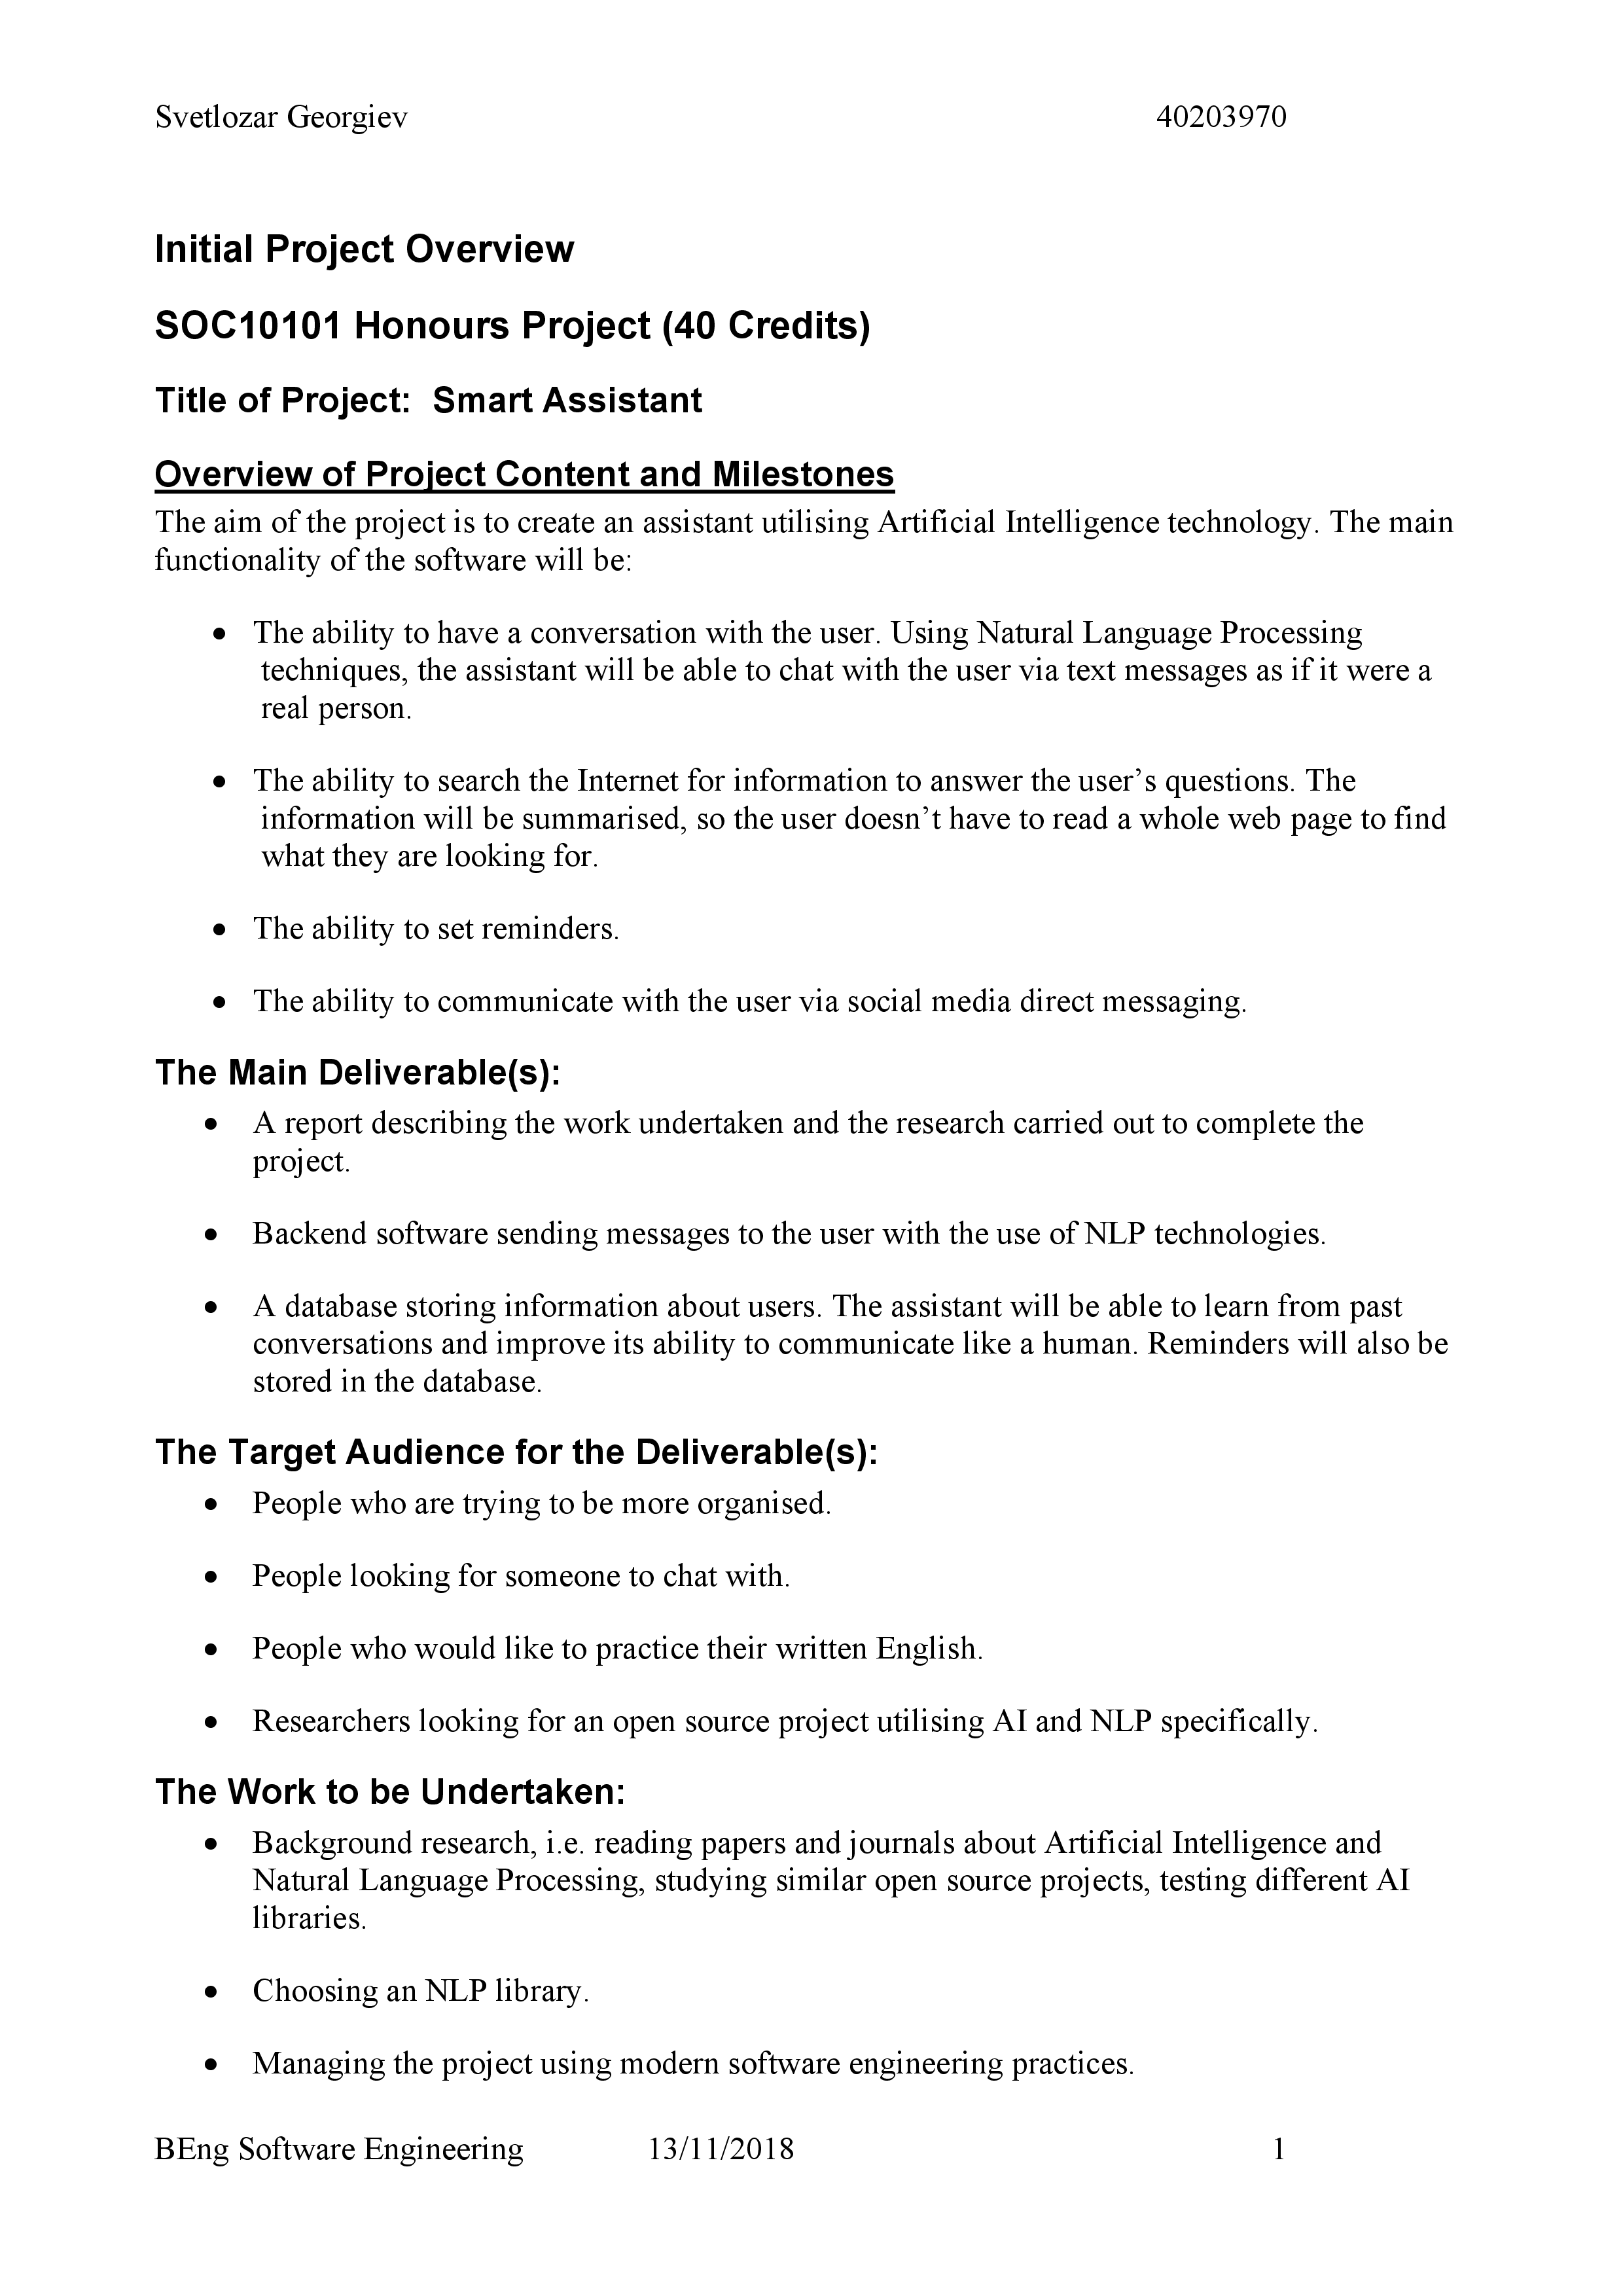
\includegraphics[width=\textwidth,height=\textheight,keepaspectratio]{IPO-0.png} % fit images to page
\newpage
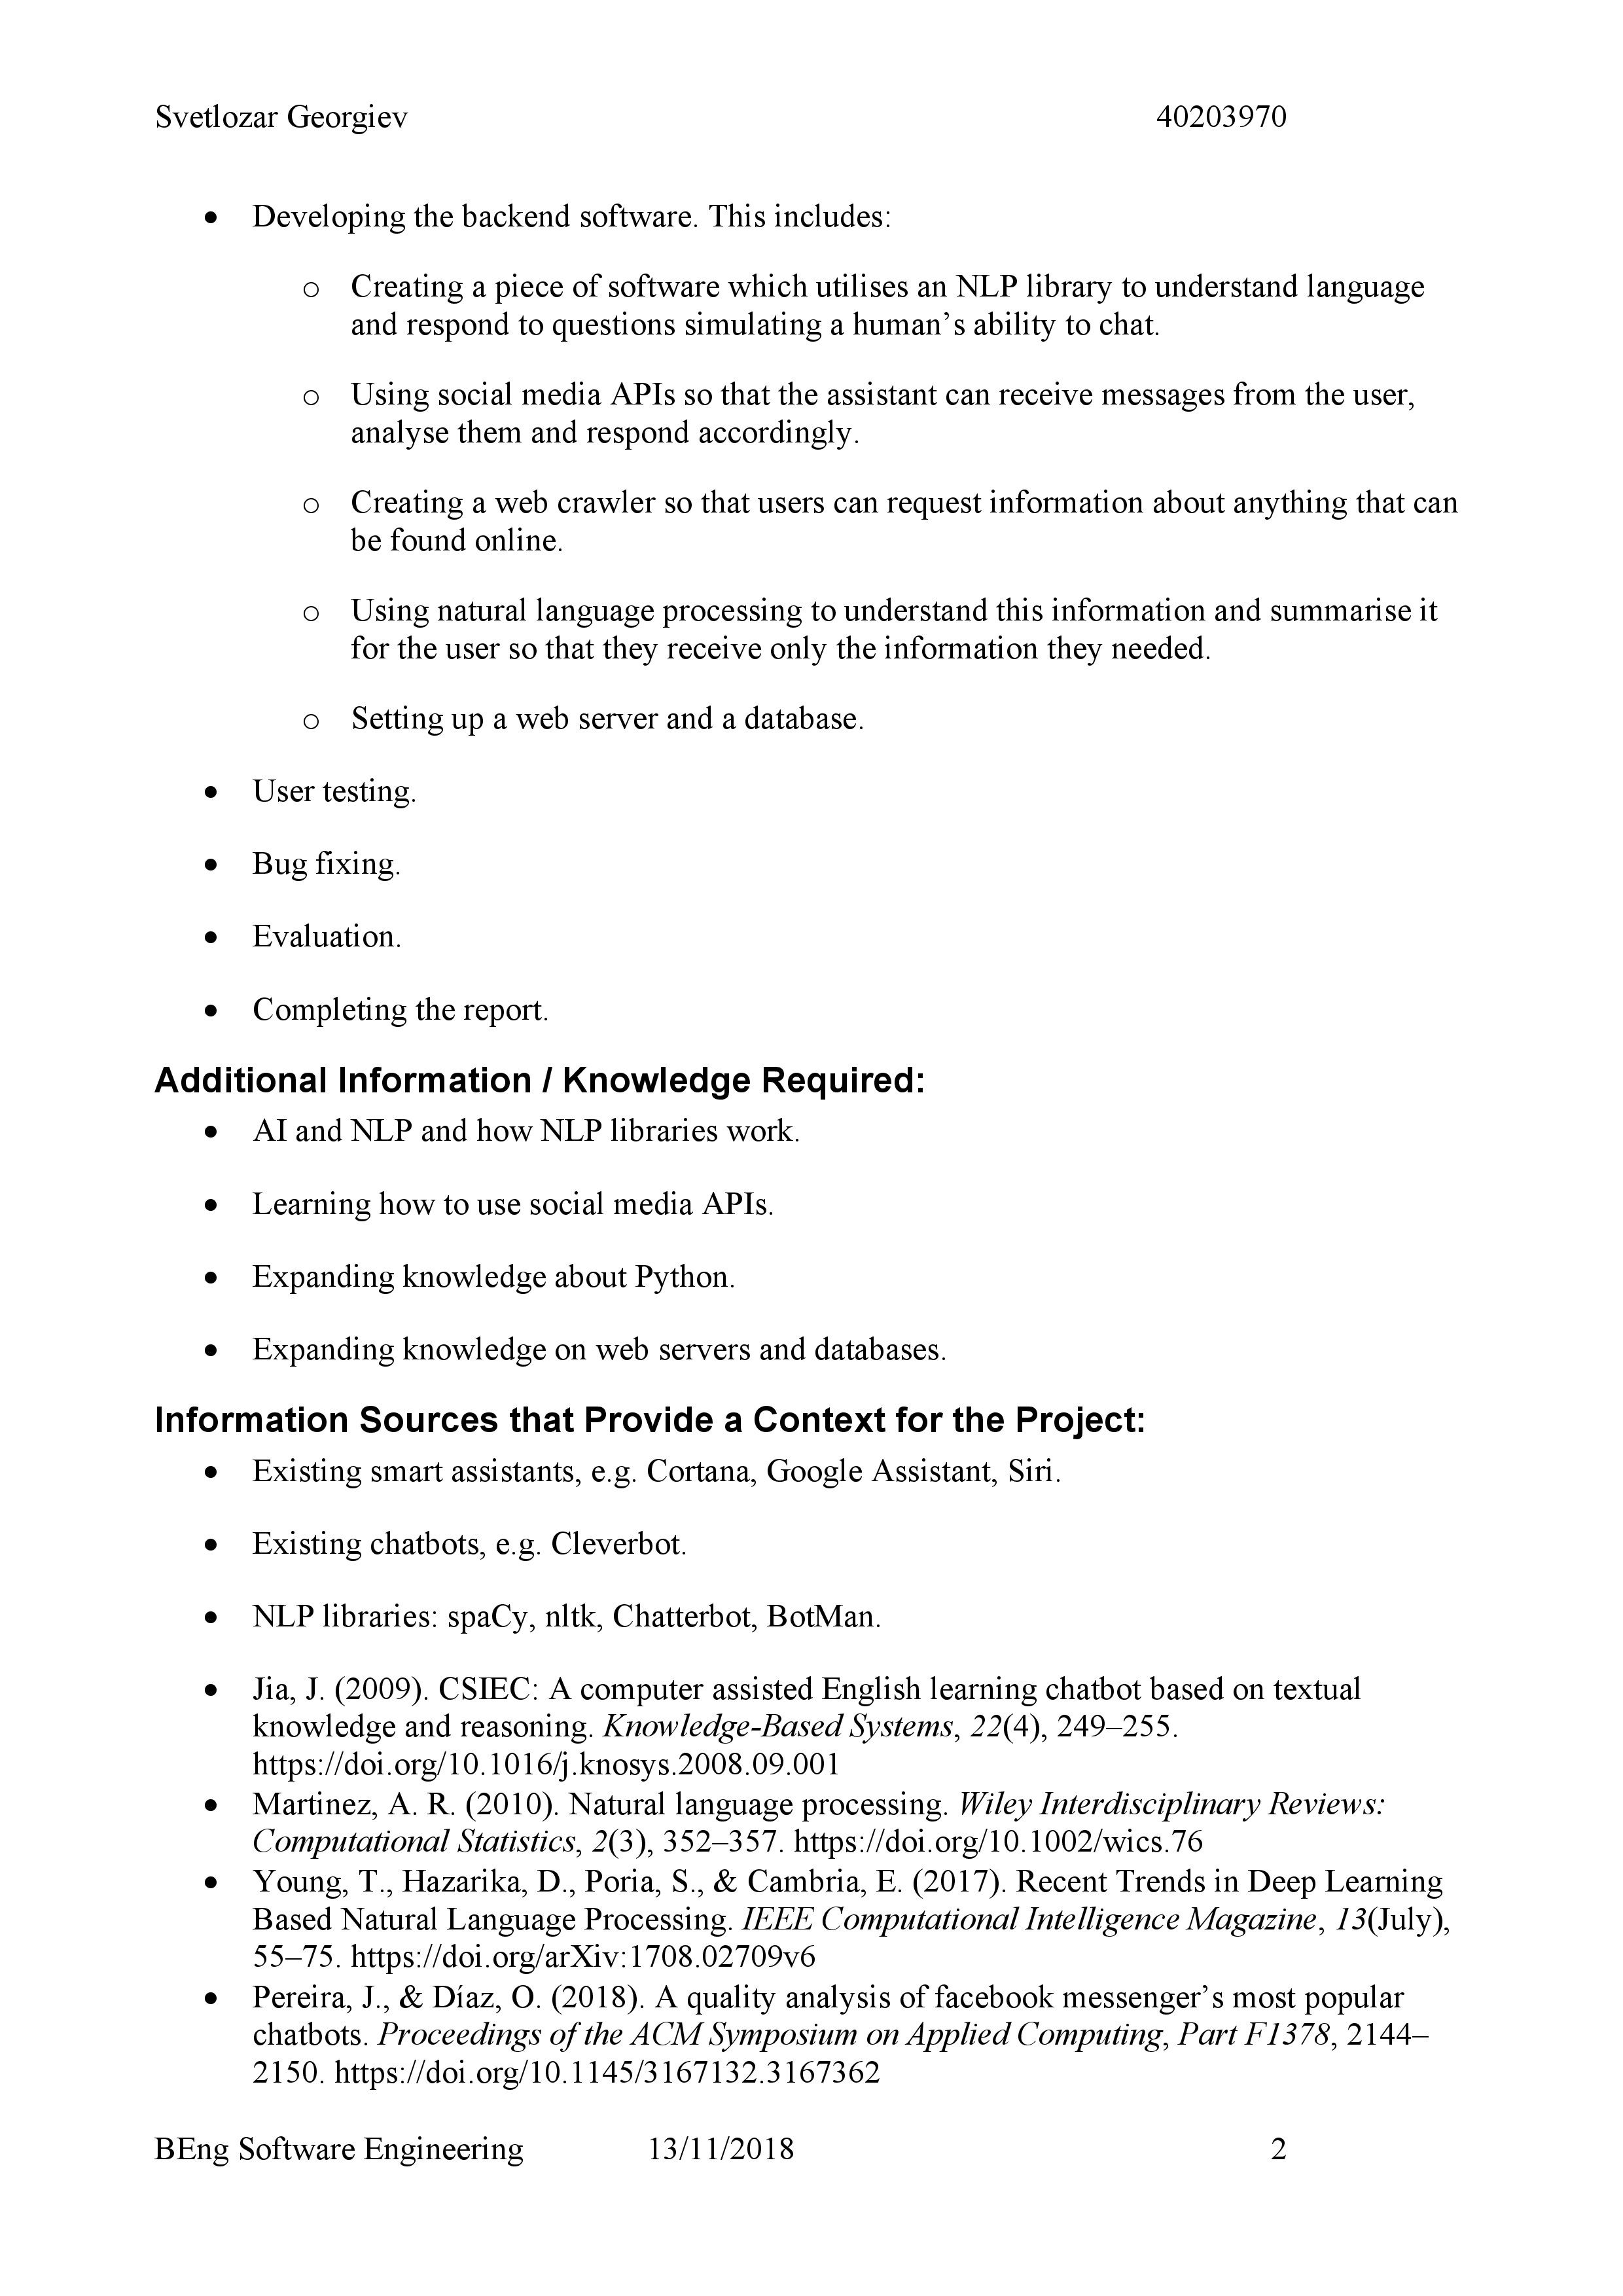
\includegraphics[width=\textwidth,height=\textheight,keepaspectratio]{IPO-1.png}
\newpage
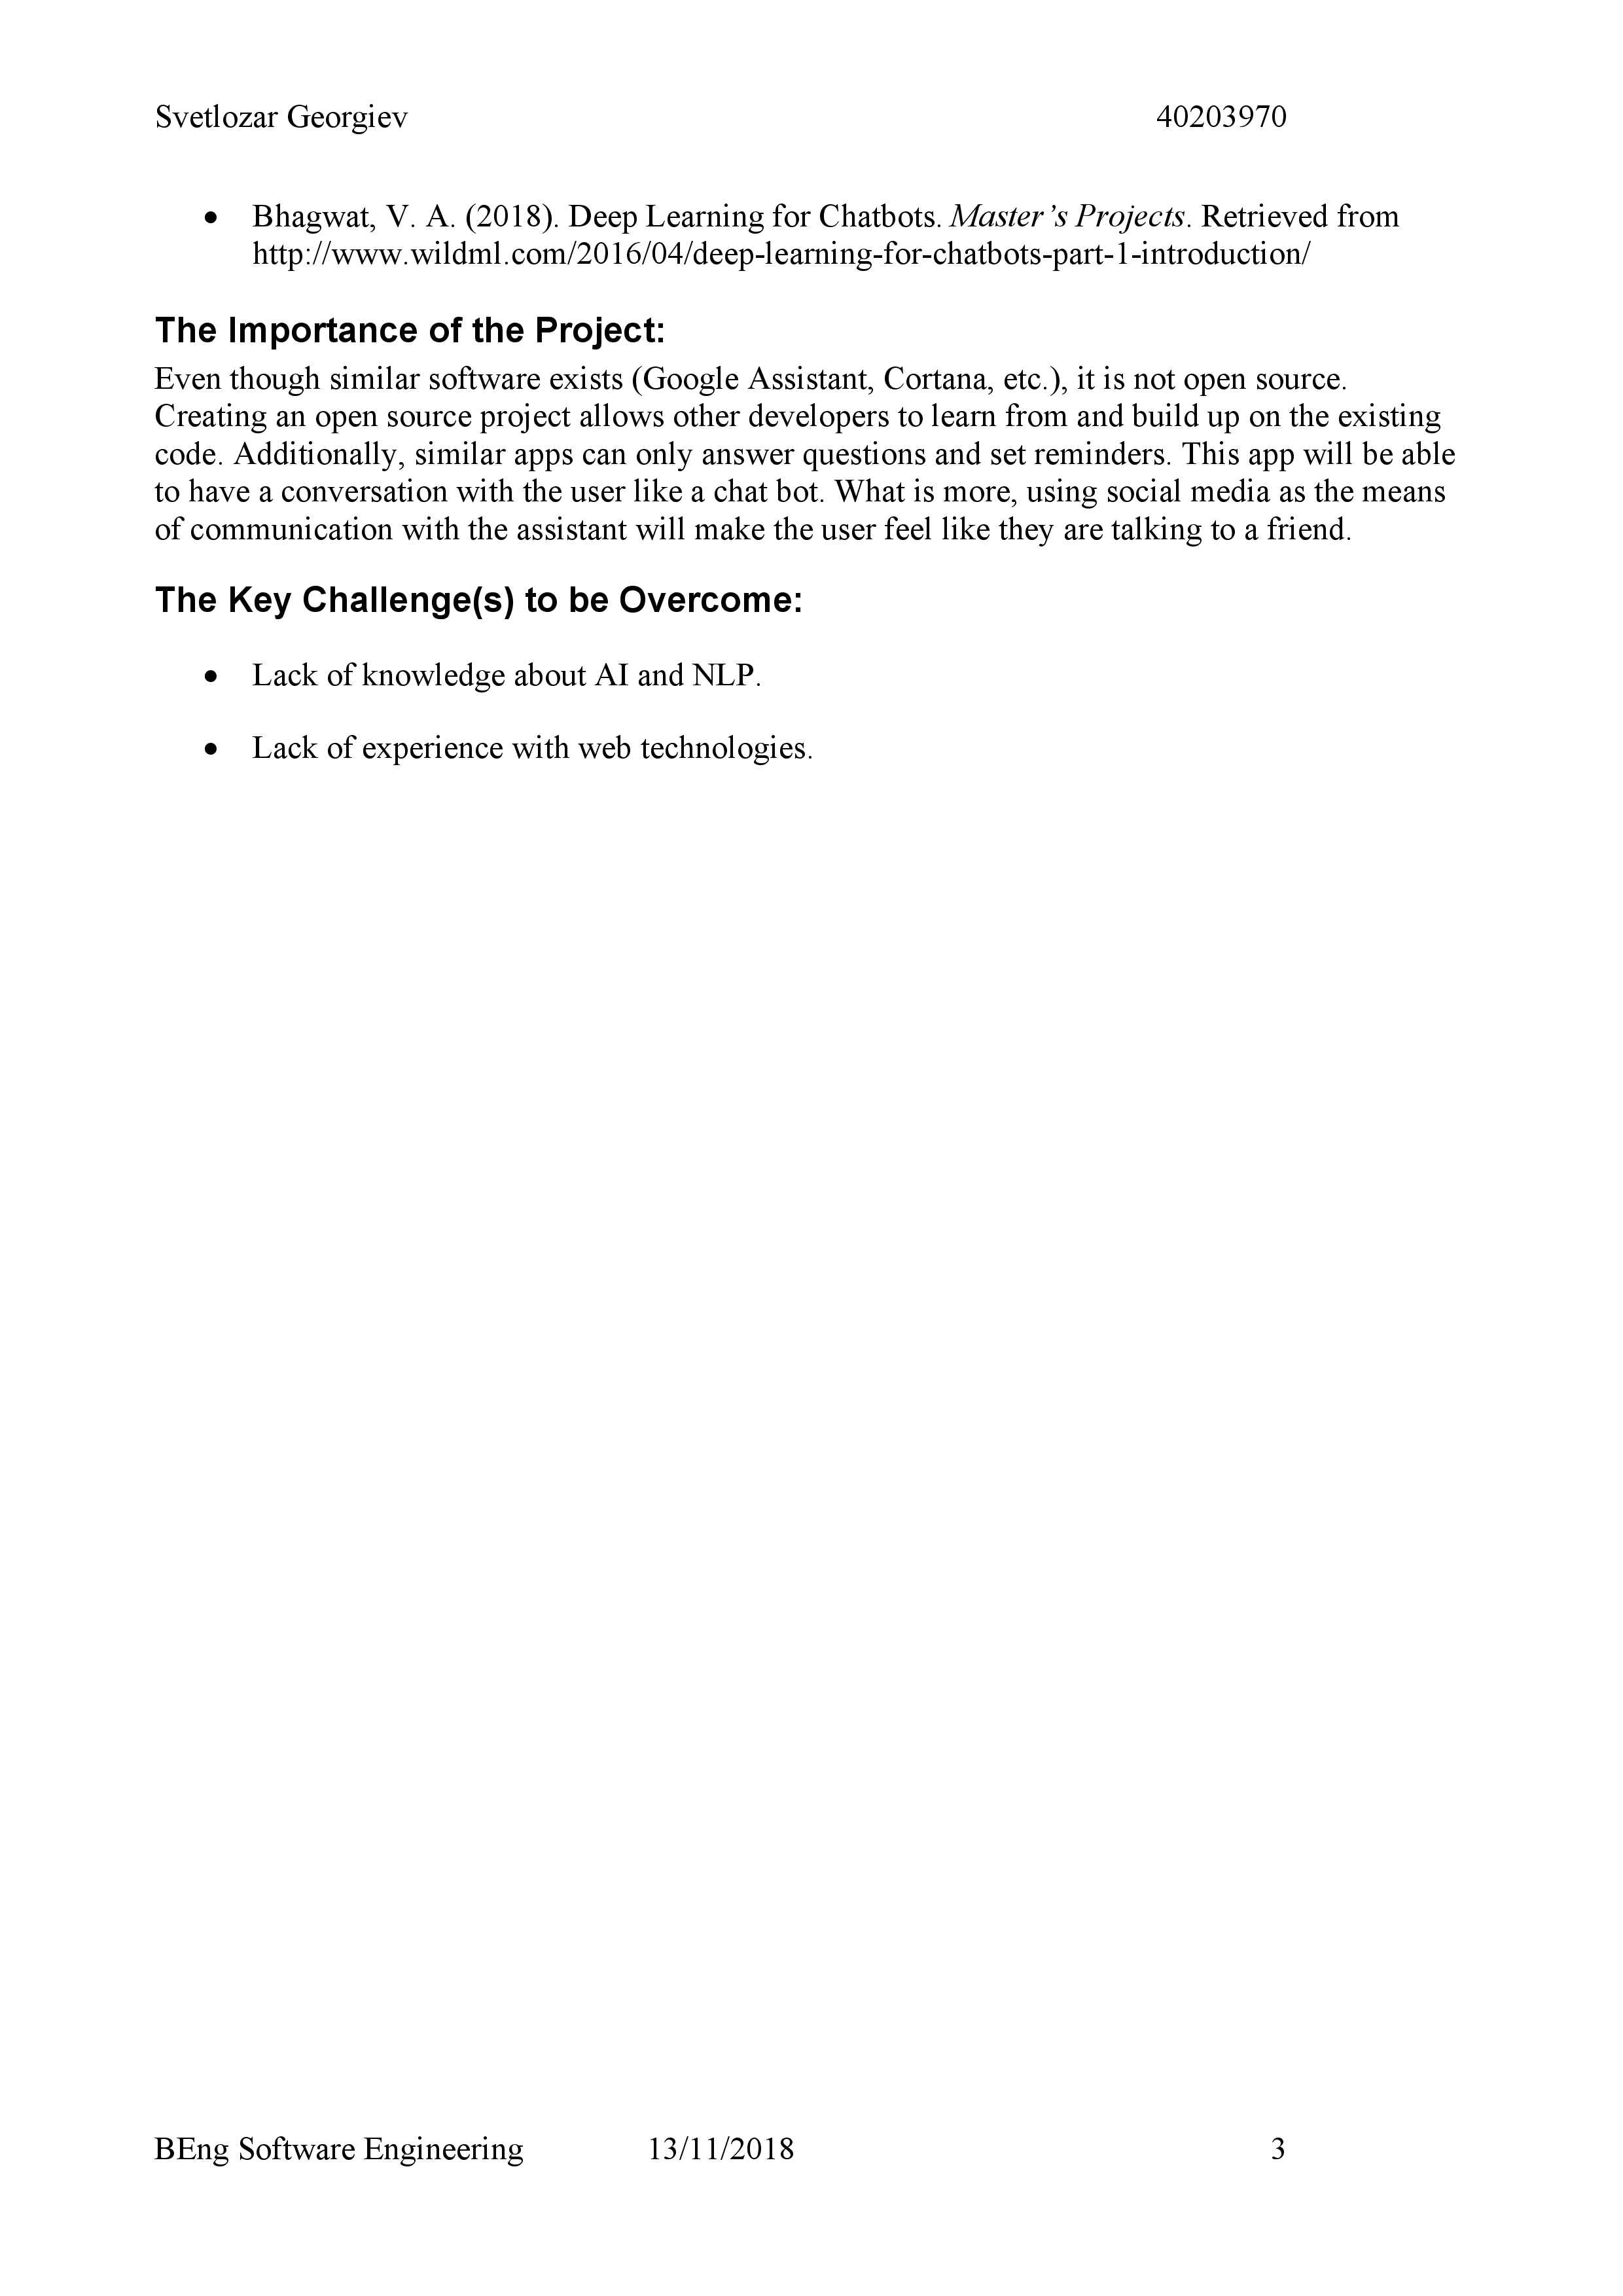
\includegraphics[width=\textwidth,height=\textheight,keepaspectratio]{IPO-2.png}

\section{Initial Project Plan}\label{app:gantt}
%\begin{figure}[b!]
%	\centering
	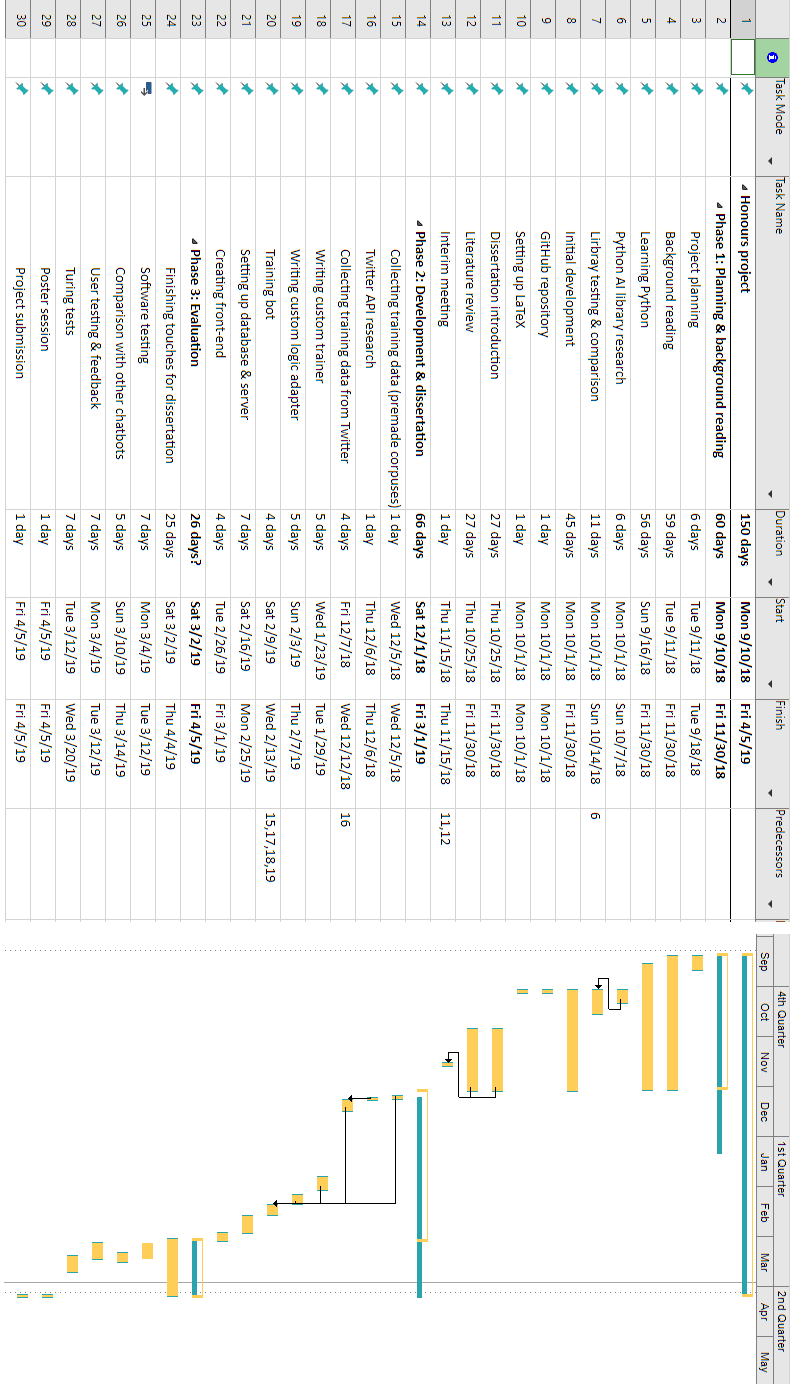
\includegraphics[width=0.8\textwidth,height=0.8\textheight]{gantt.png}
%\end{figure}


\newpage
\section{Diary Sheets}
% first semester
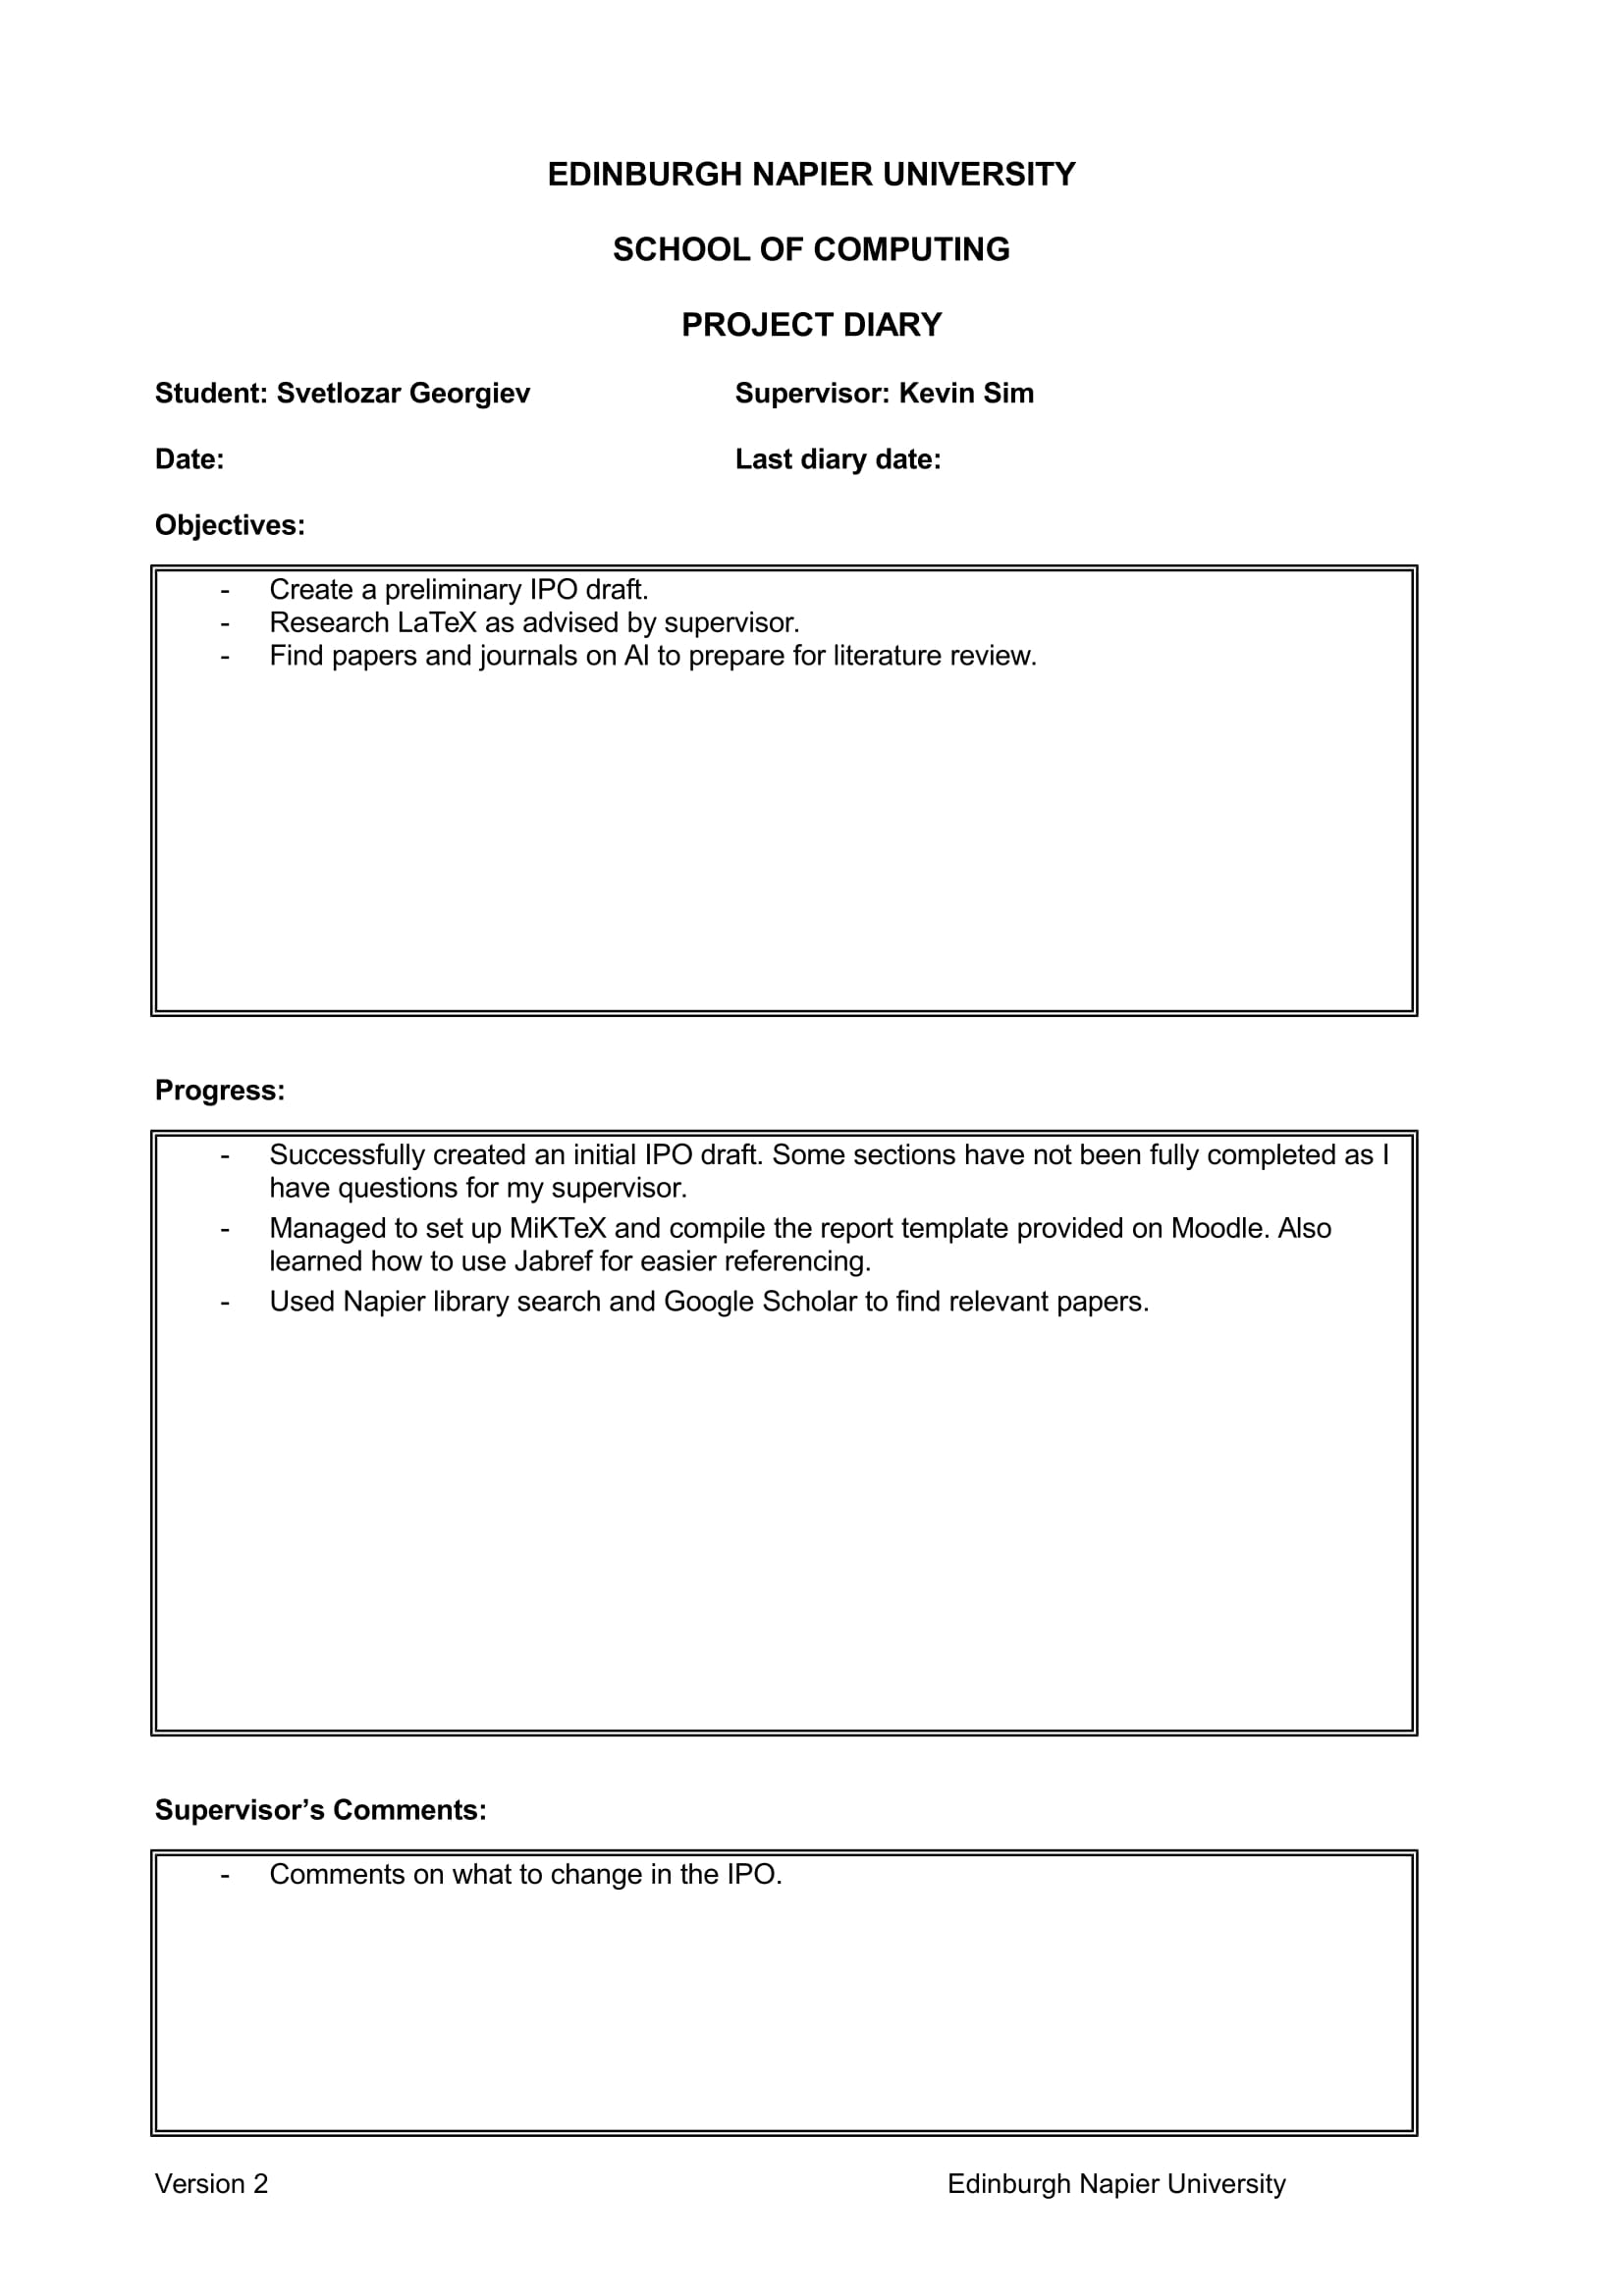
\includegraphics[width=\textwidth,height=\textheight,keepaspectratio]{week2.jpg} % fit images to page
\newpage
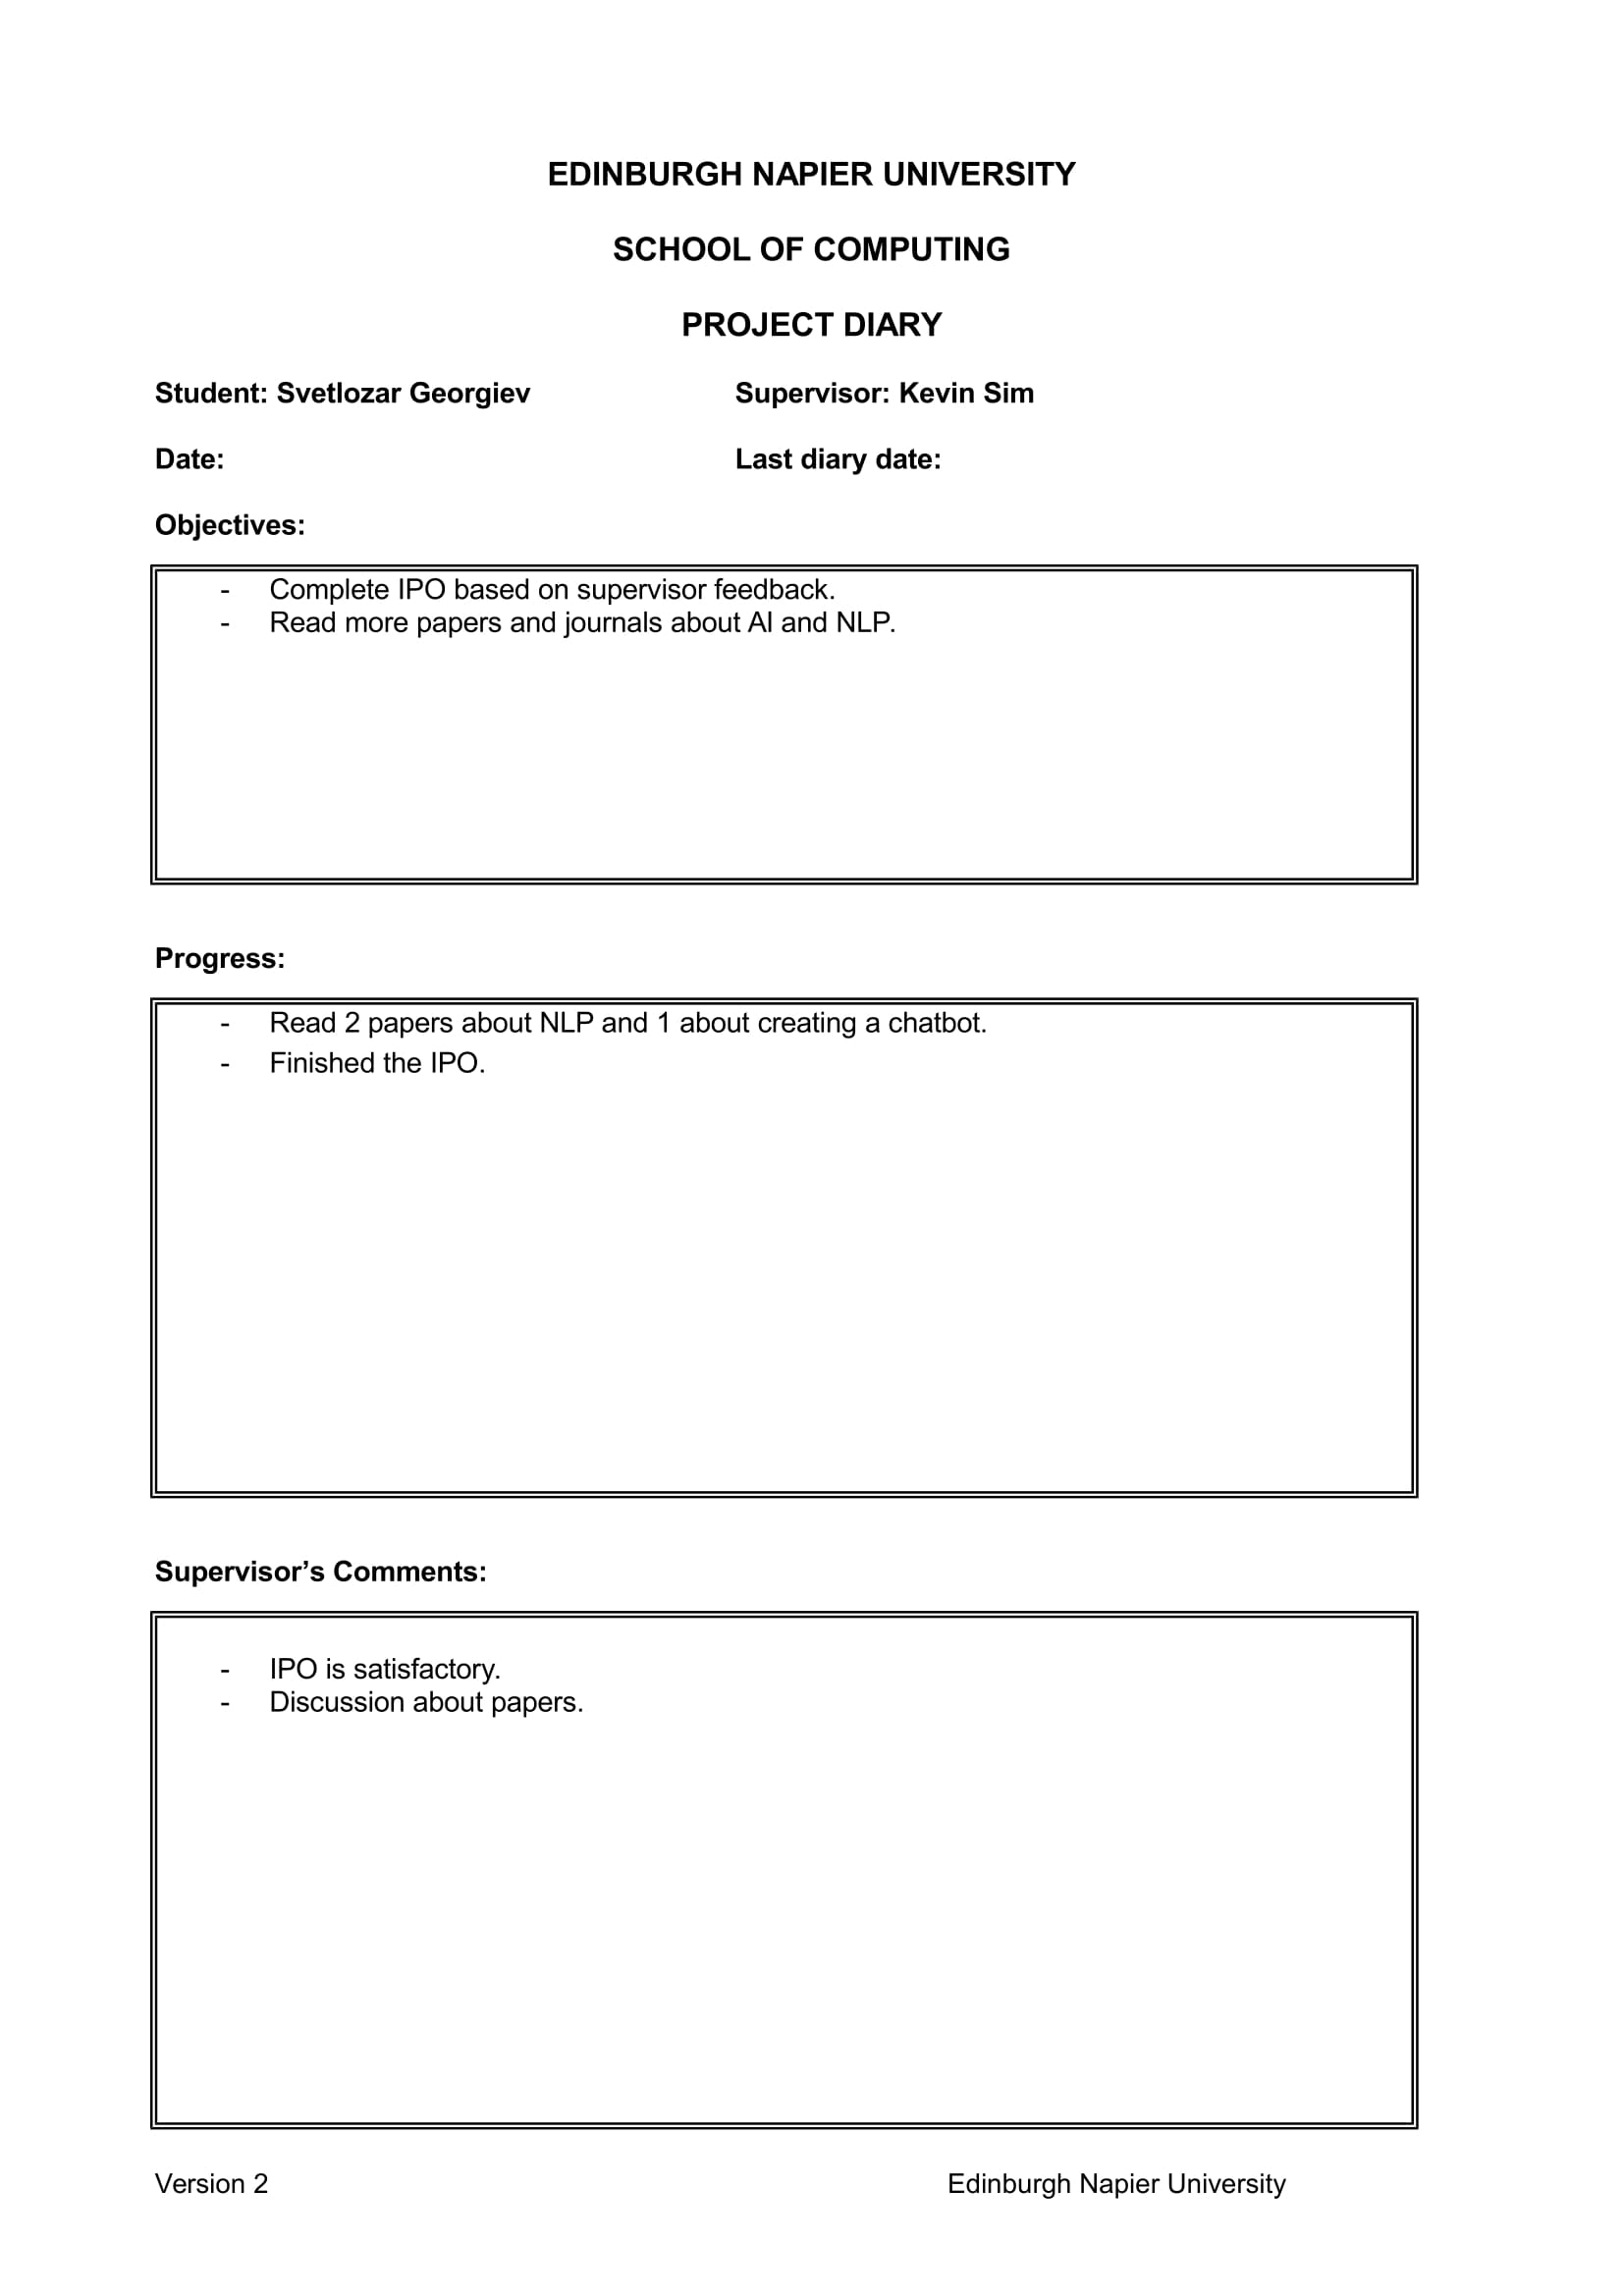
\includegraphics[width=\textwidth,height=\textheight,keepaspectratio]{week3.jpg}
\newpage
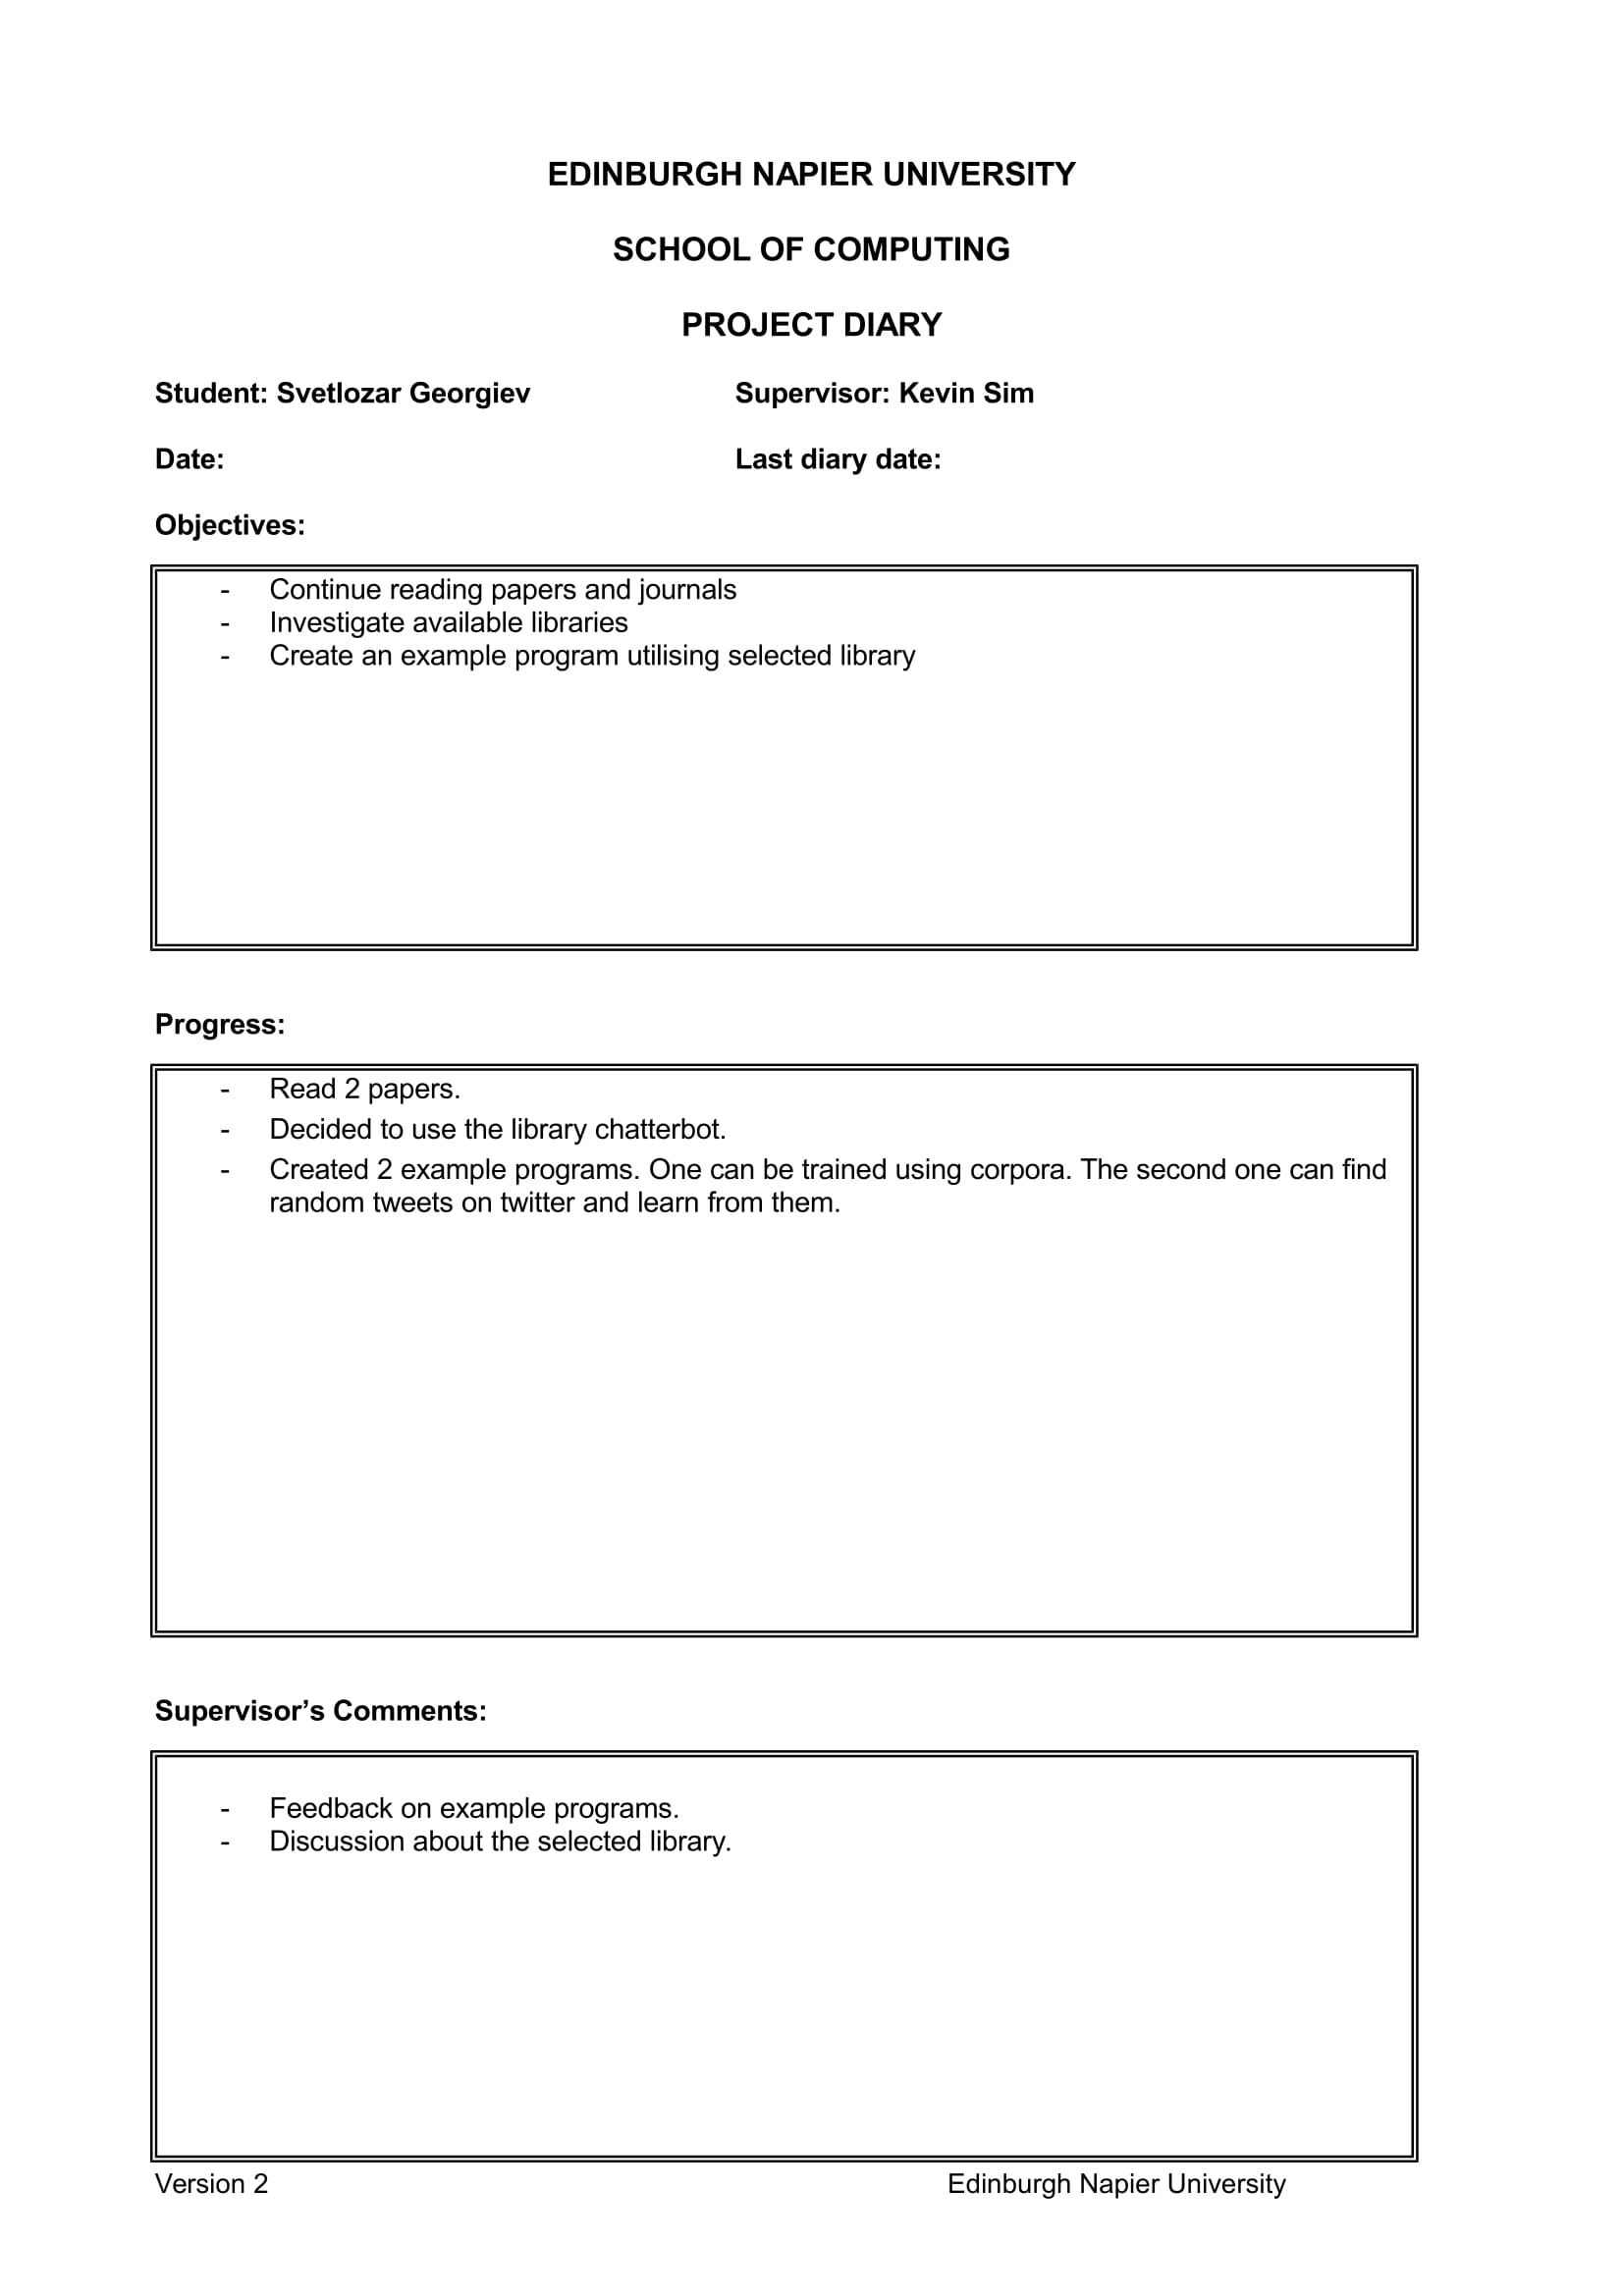
\includegraphics[width=\textwidth,height=\textheight,keepaspectratio]{week4.jpg}
\newpage
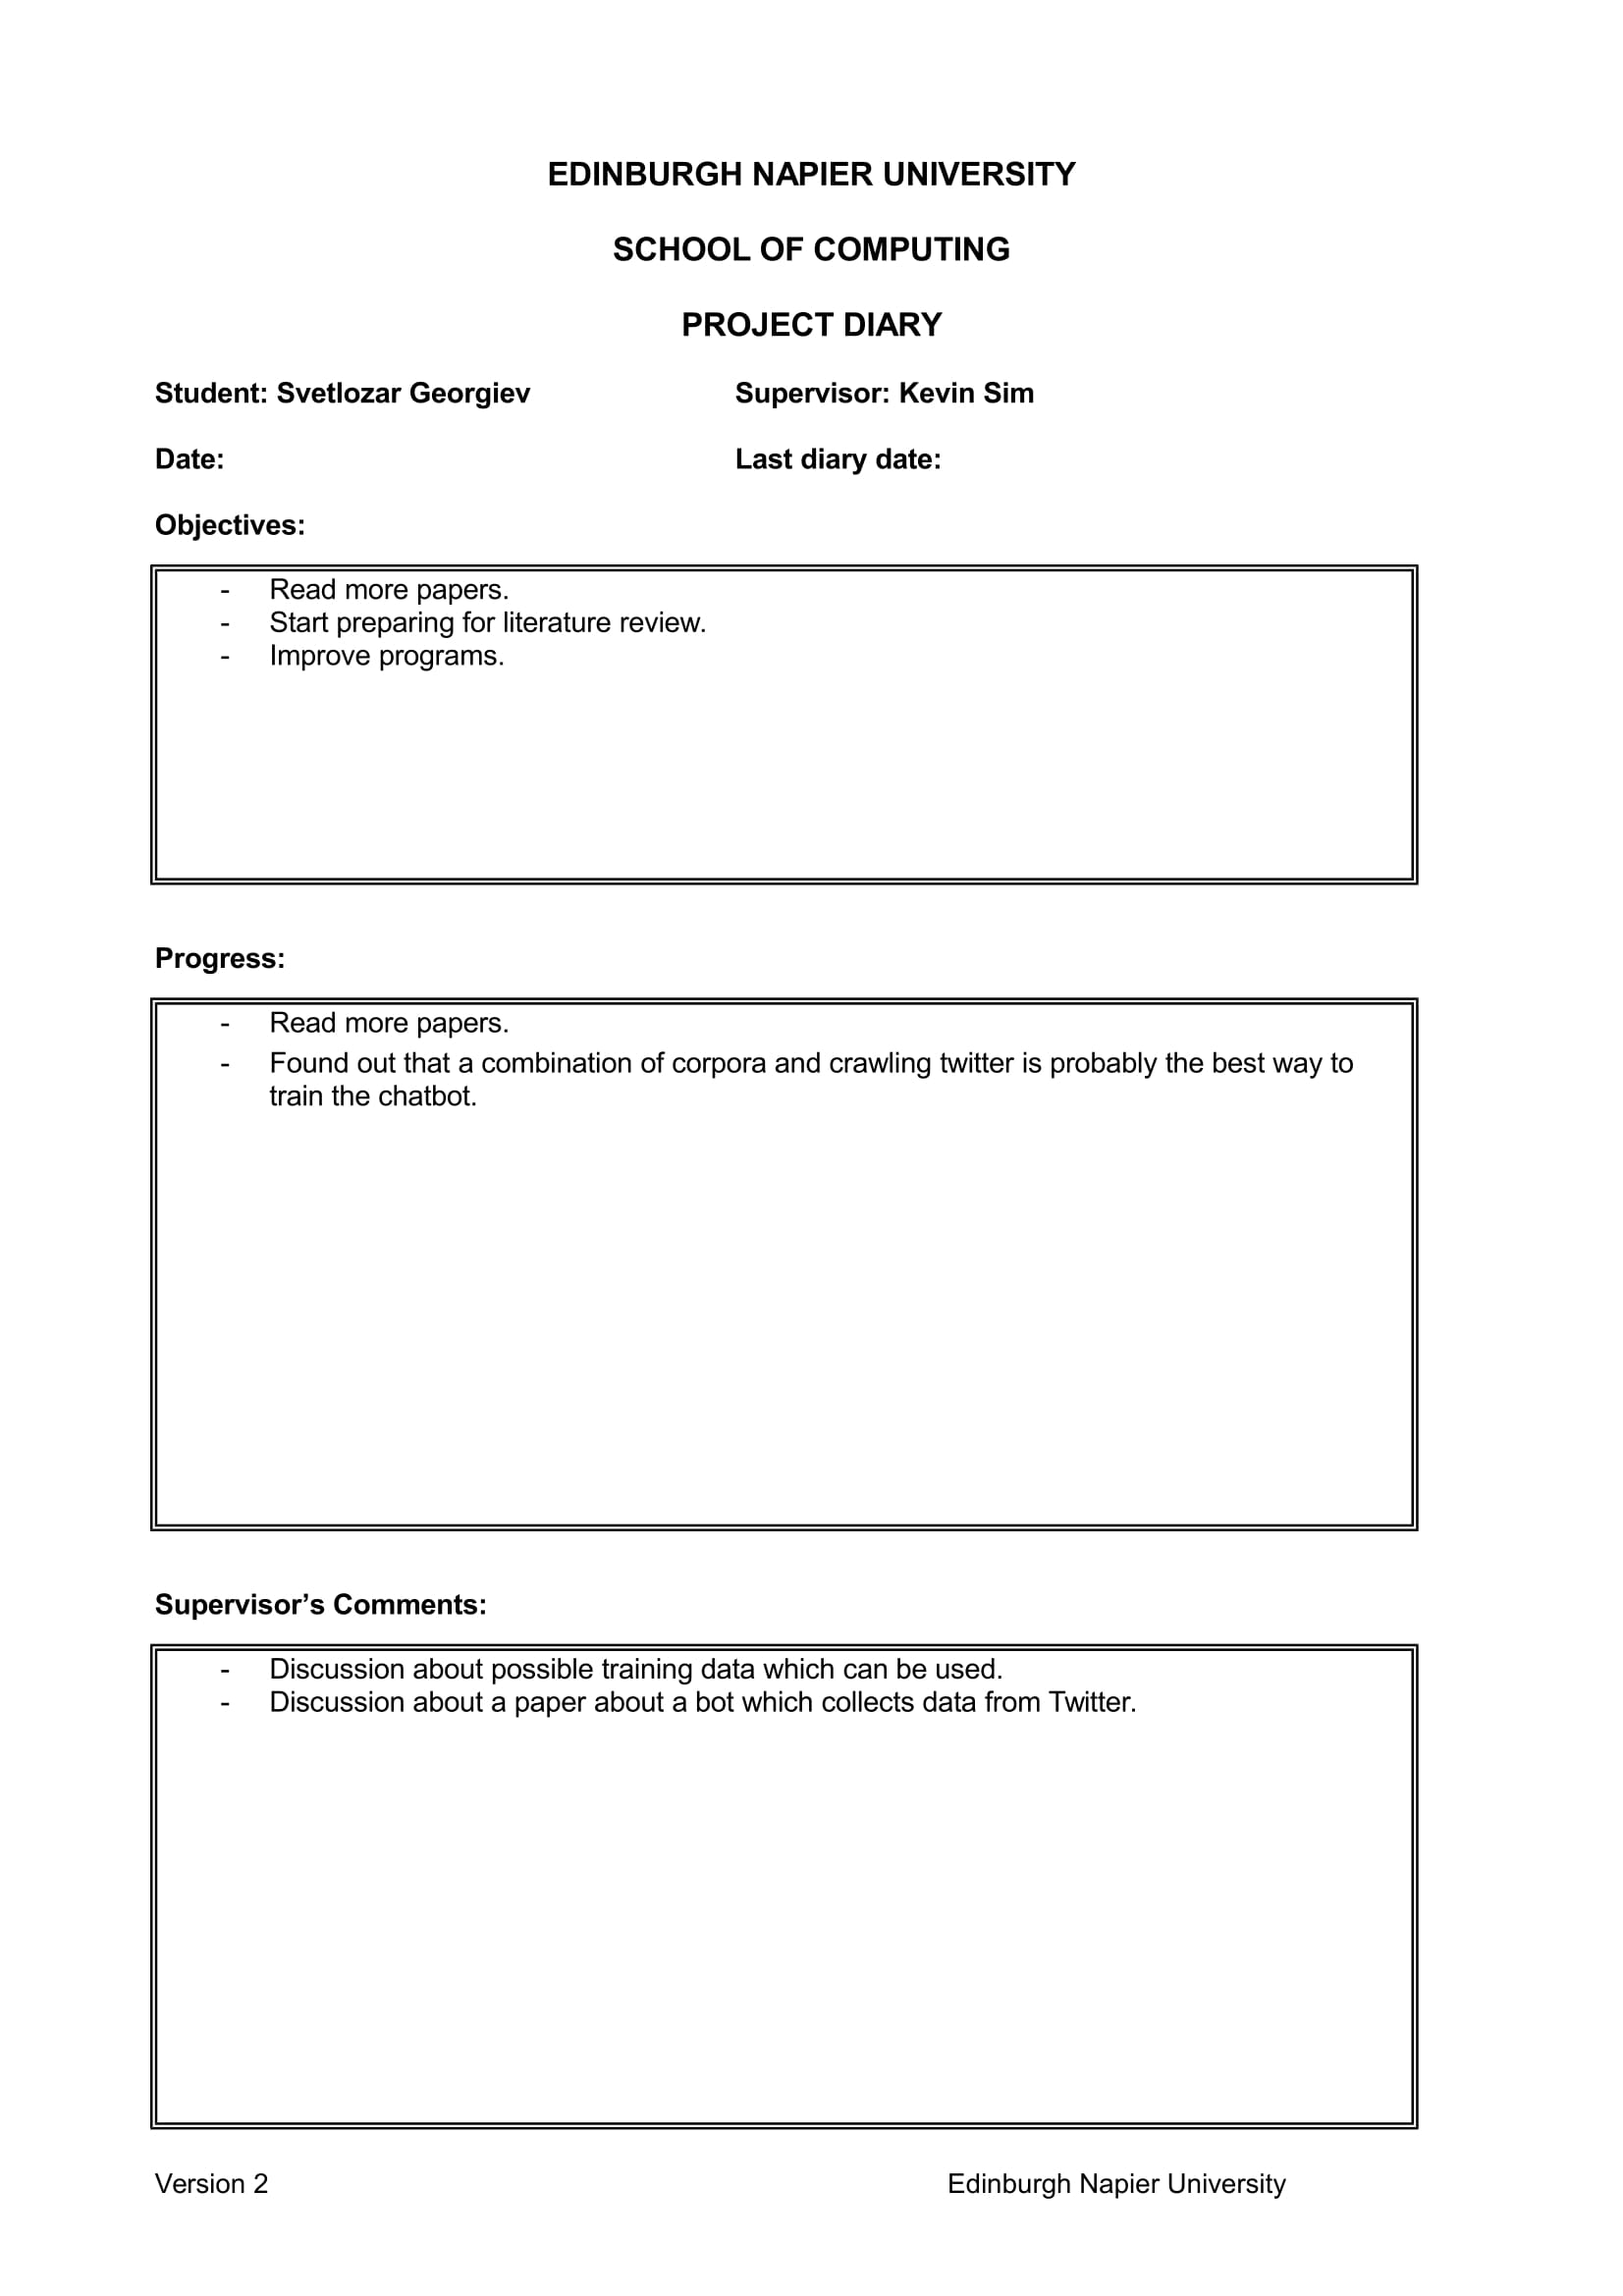
\includegraphics[width=\textwidth,height=\textheight,keepaspectratio]{week5.jpg}
\newpage
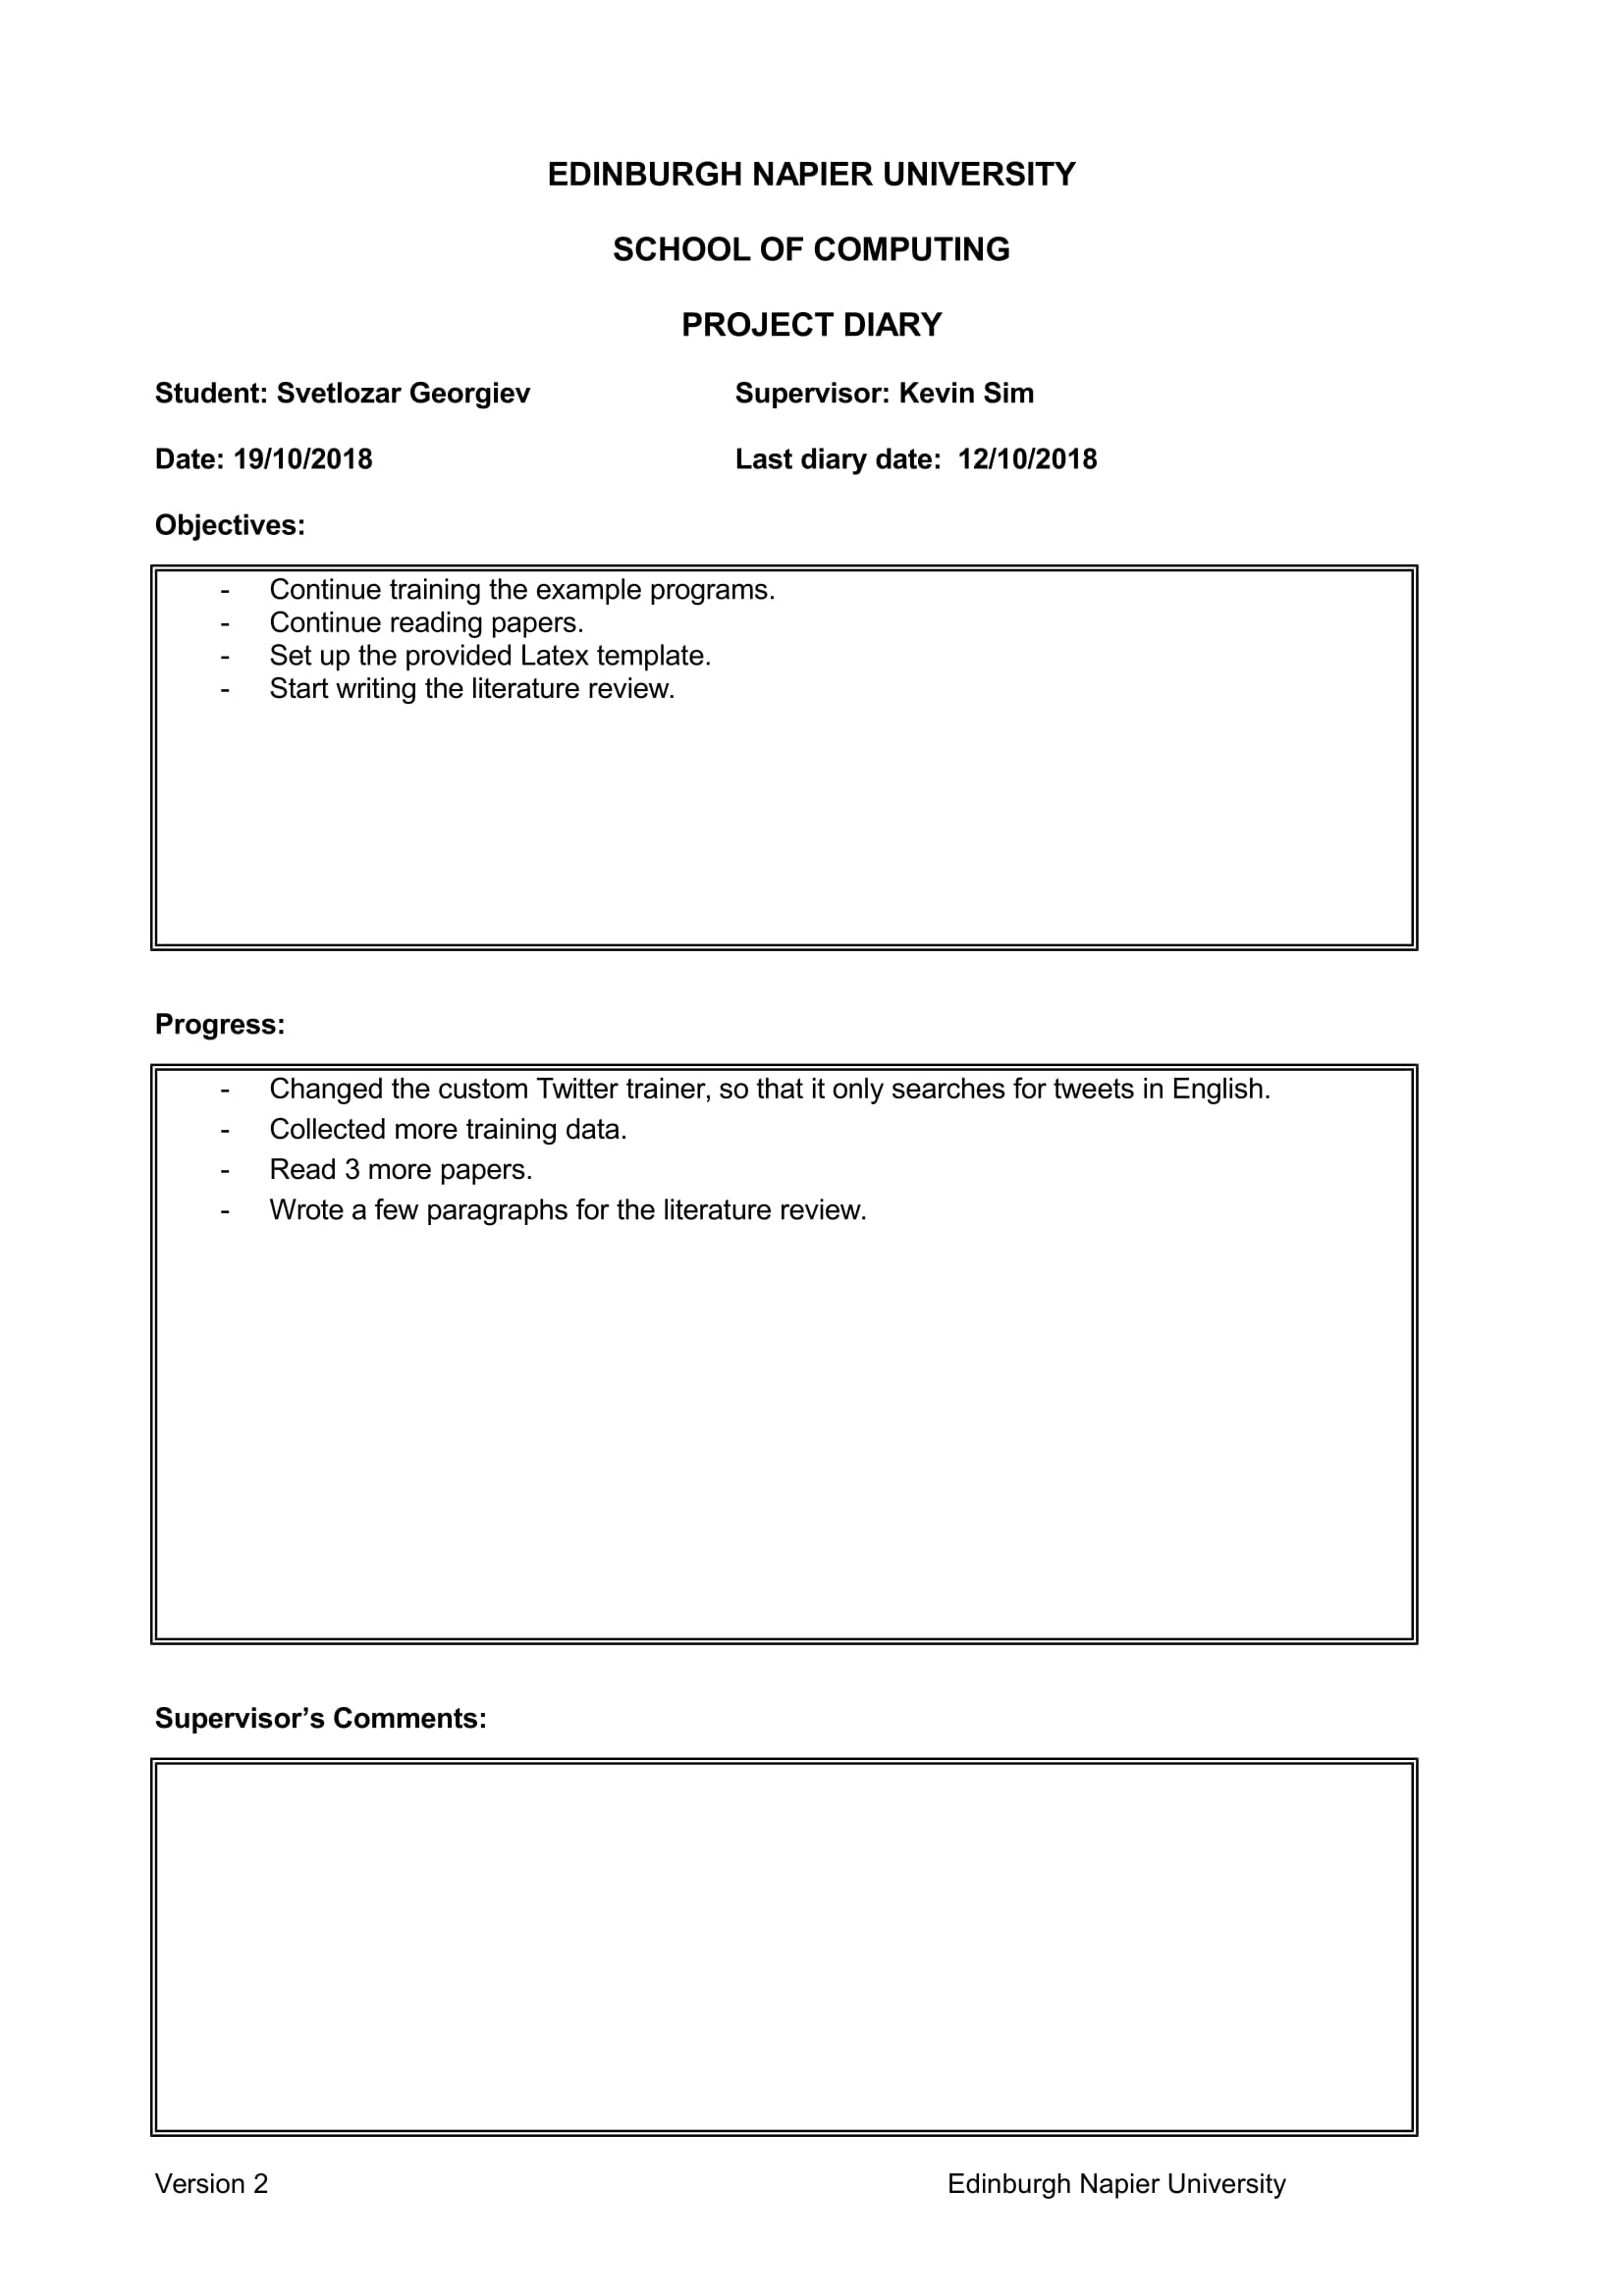
\includegraphics[width=\textwidth,height=\textheight,keepaspectratio]{week6.jpg}
\newpage
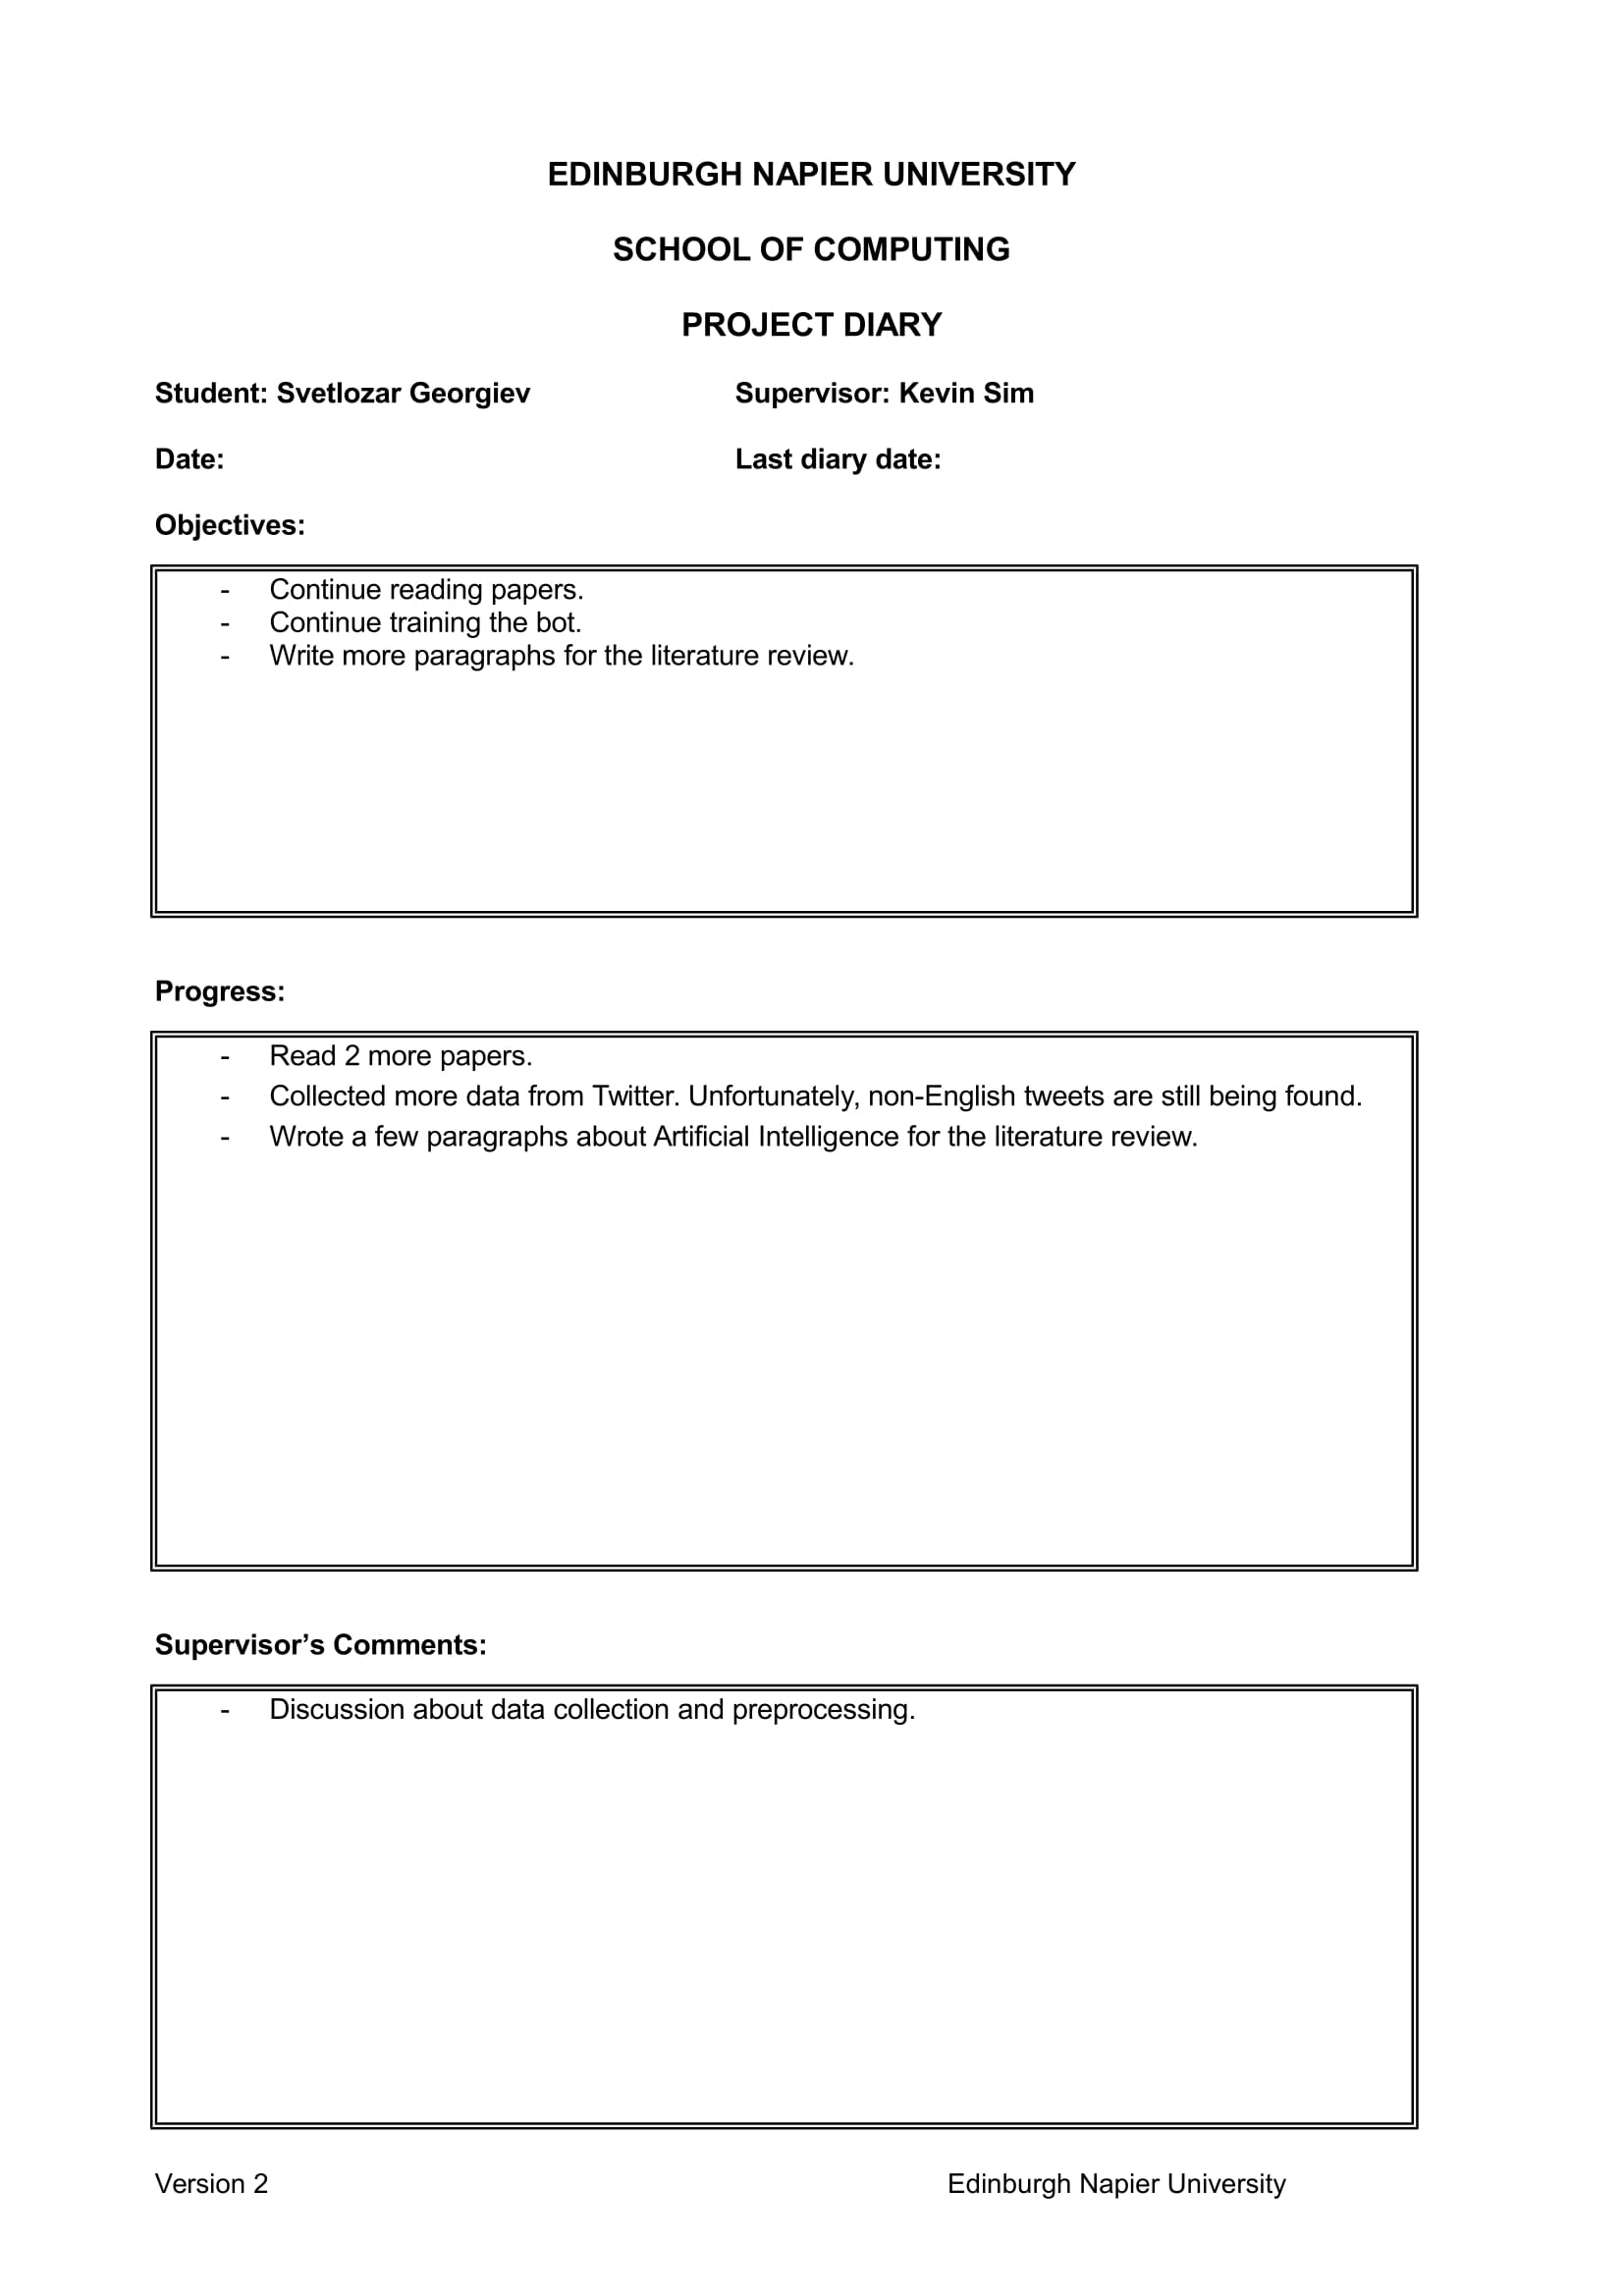
\includegraphics[width=\textwidth,height=\textheight,keepaspectratio]{week7.jpg}
\newpage
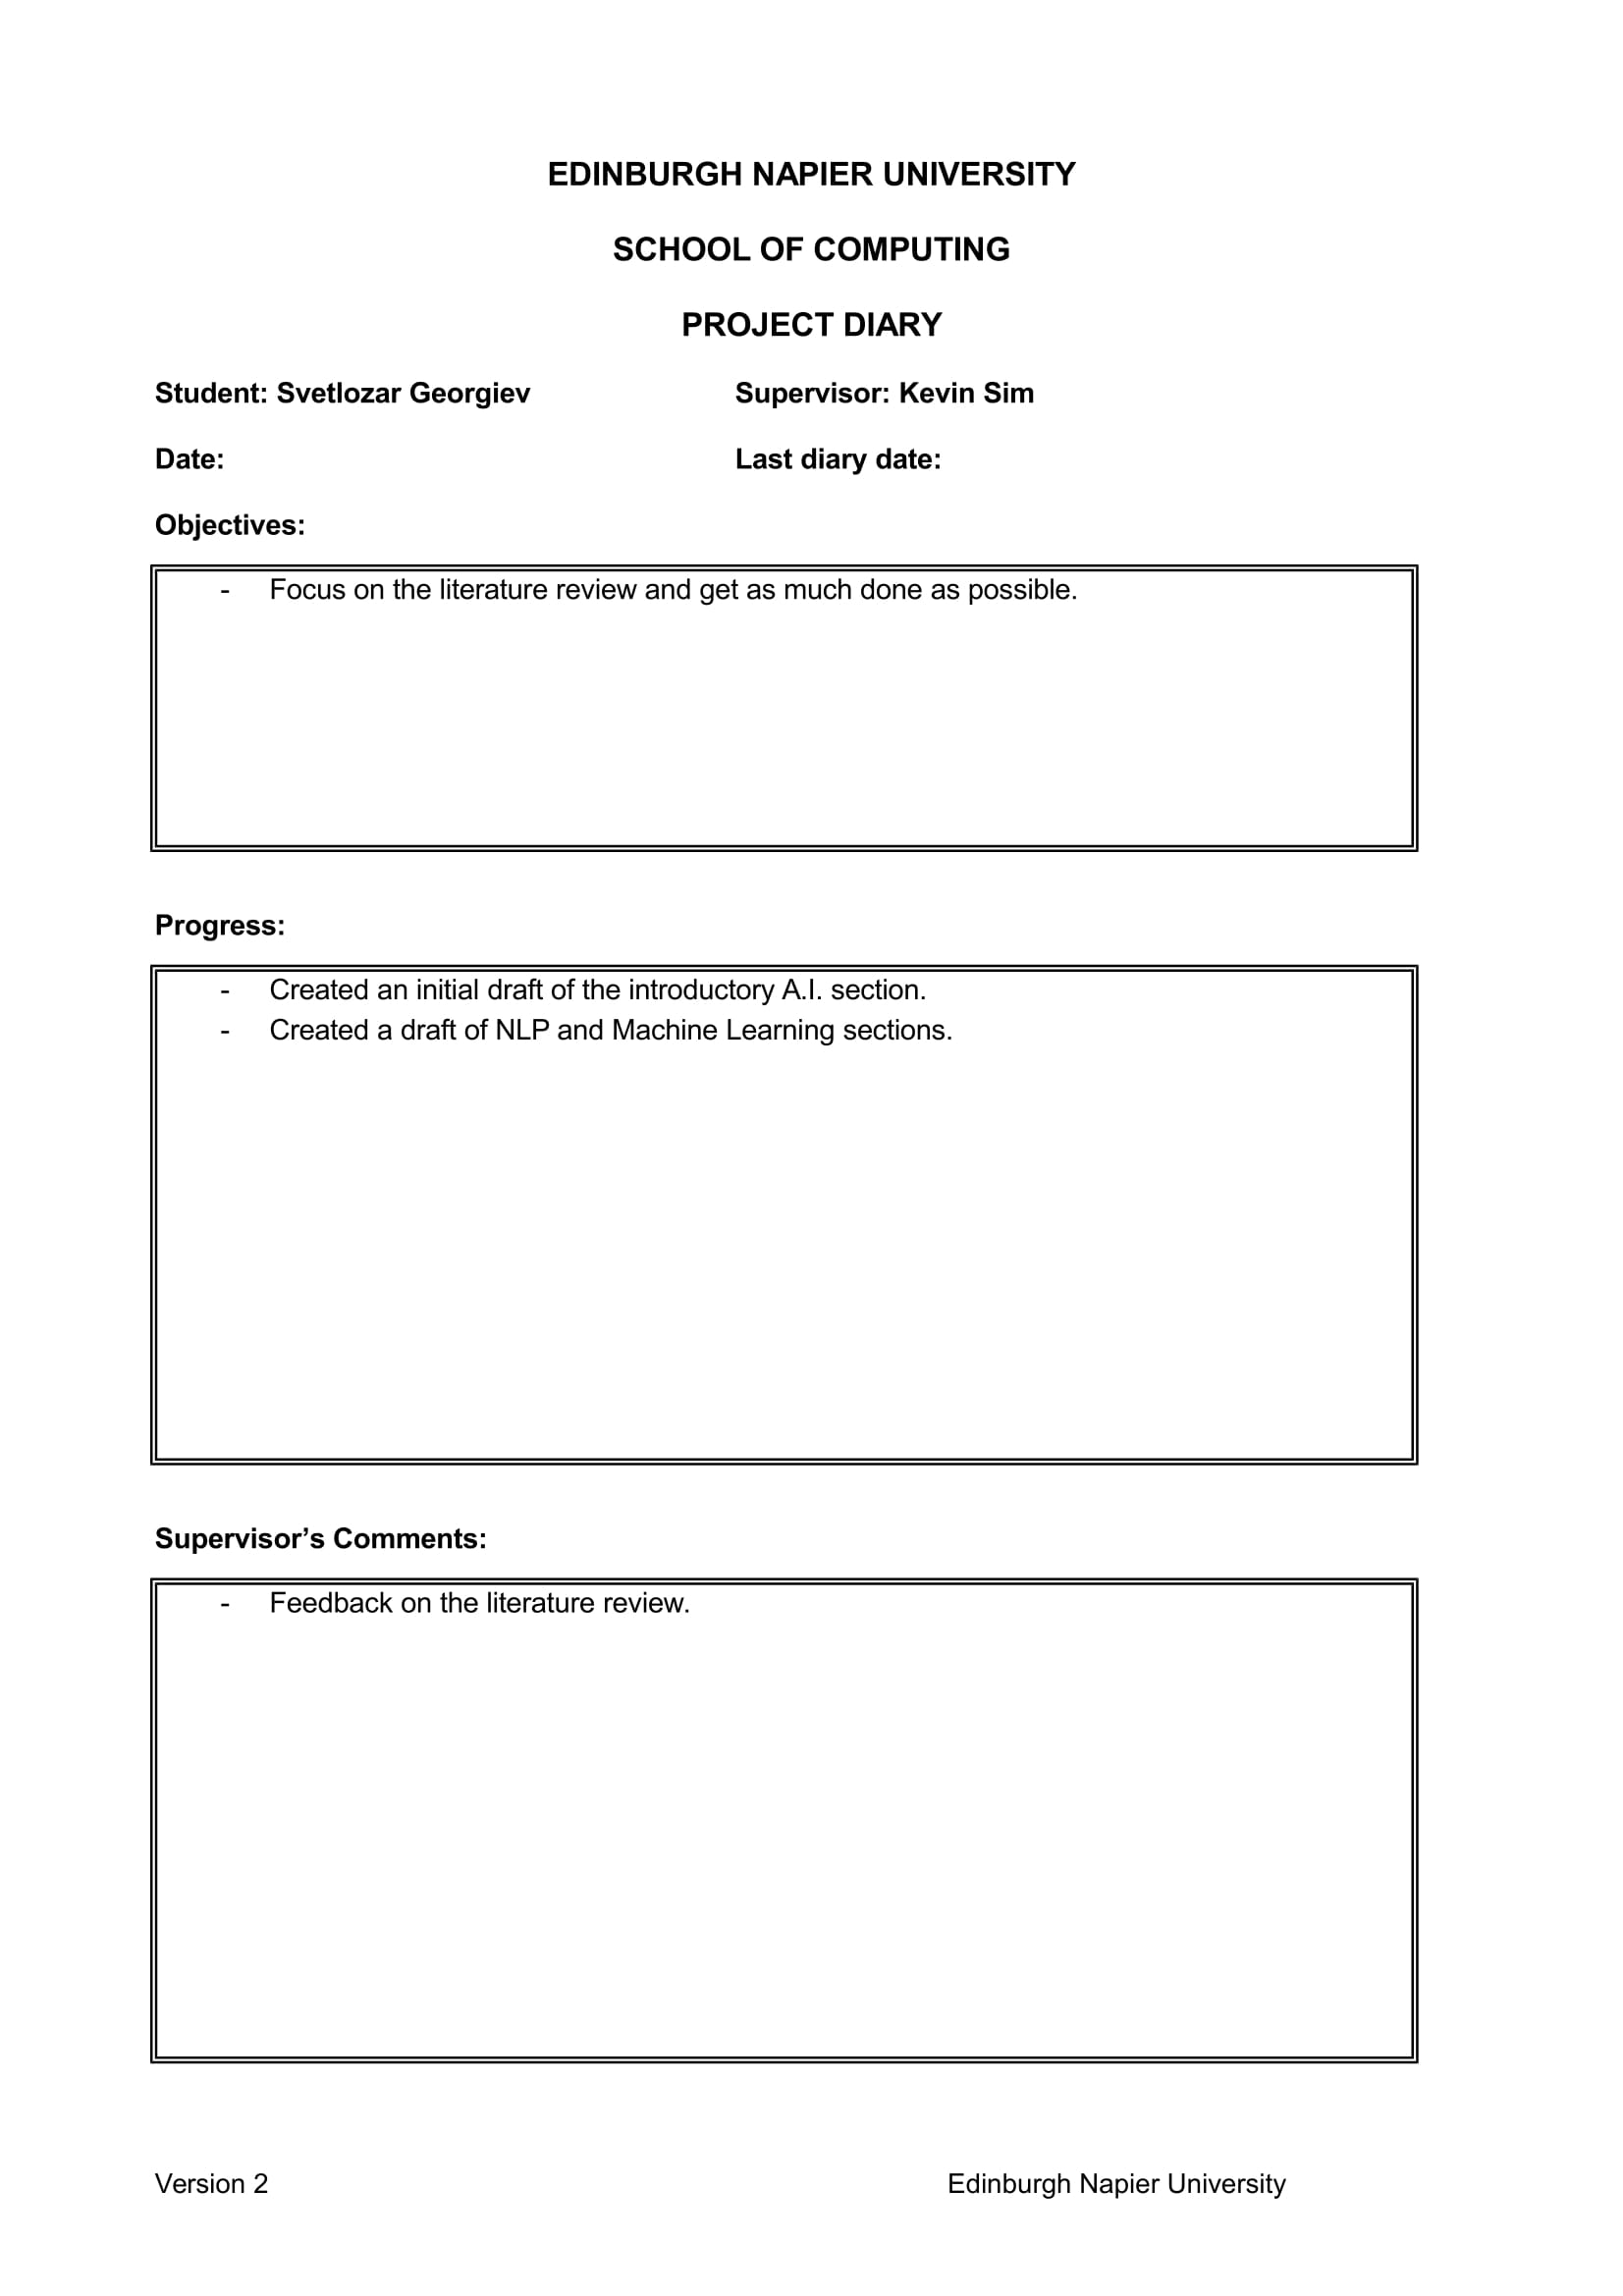
\includegraphics[width=\textwidth,height=\textheight,keepaspectratio]{week8.jpg}
\newpage
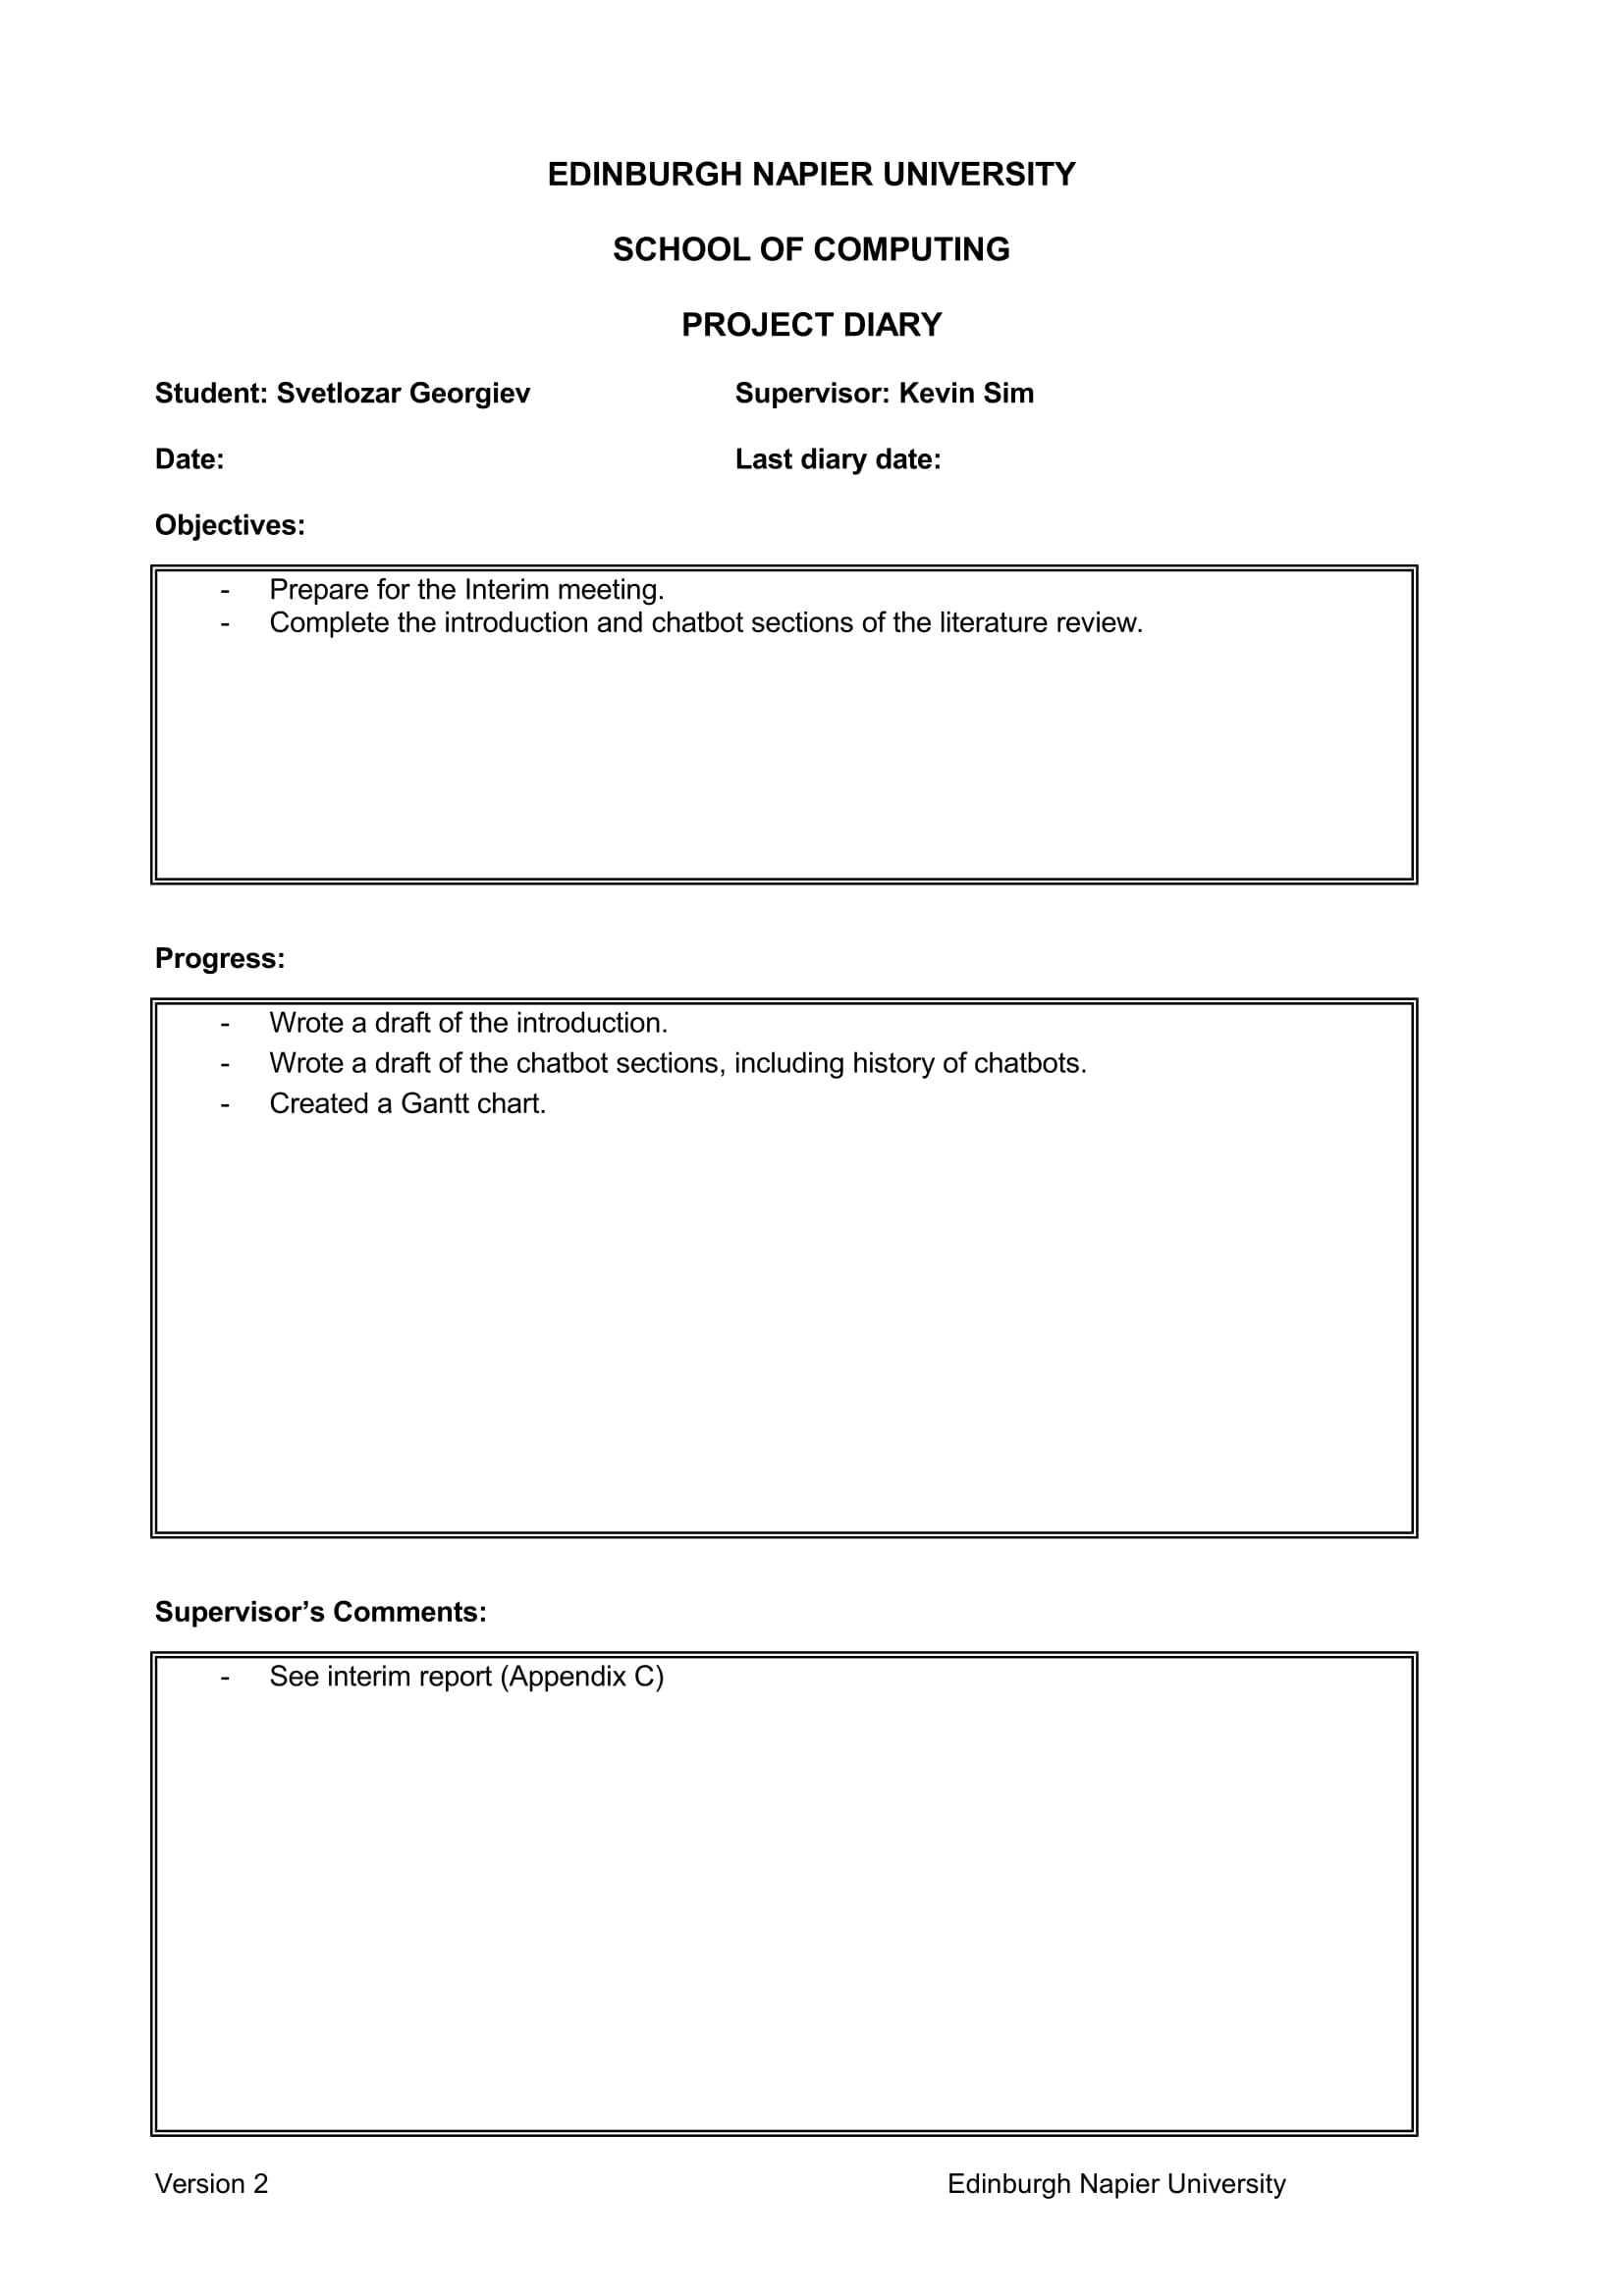
\includegraphics[width=\textwidth,height=\textheight,keepaspectratio]{week9.jpg}

% second semester
\newpage
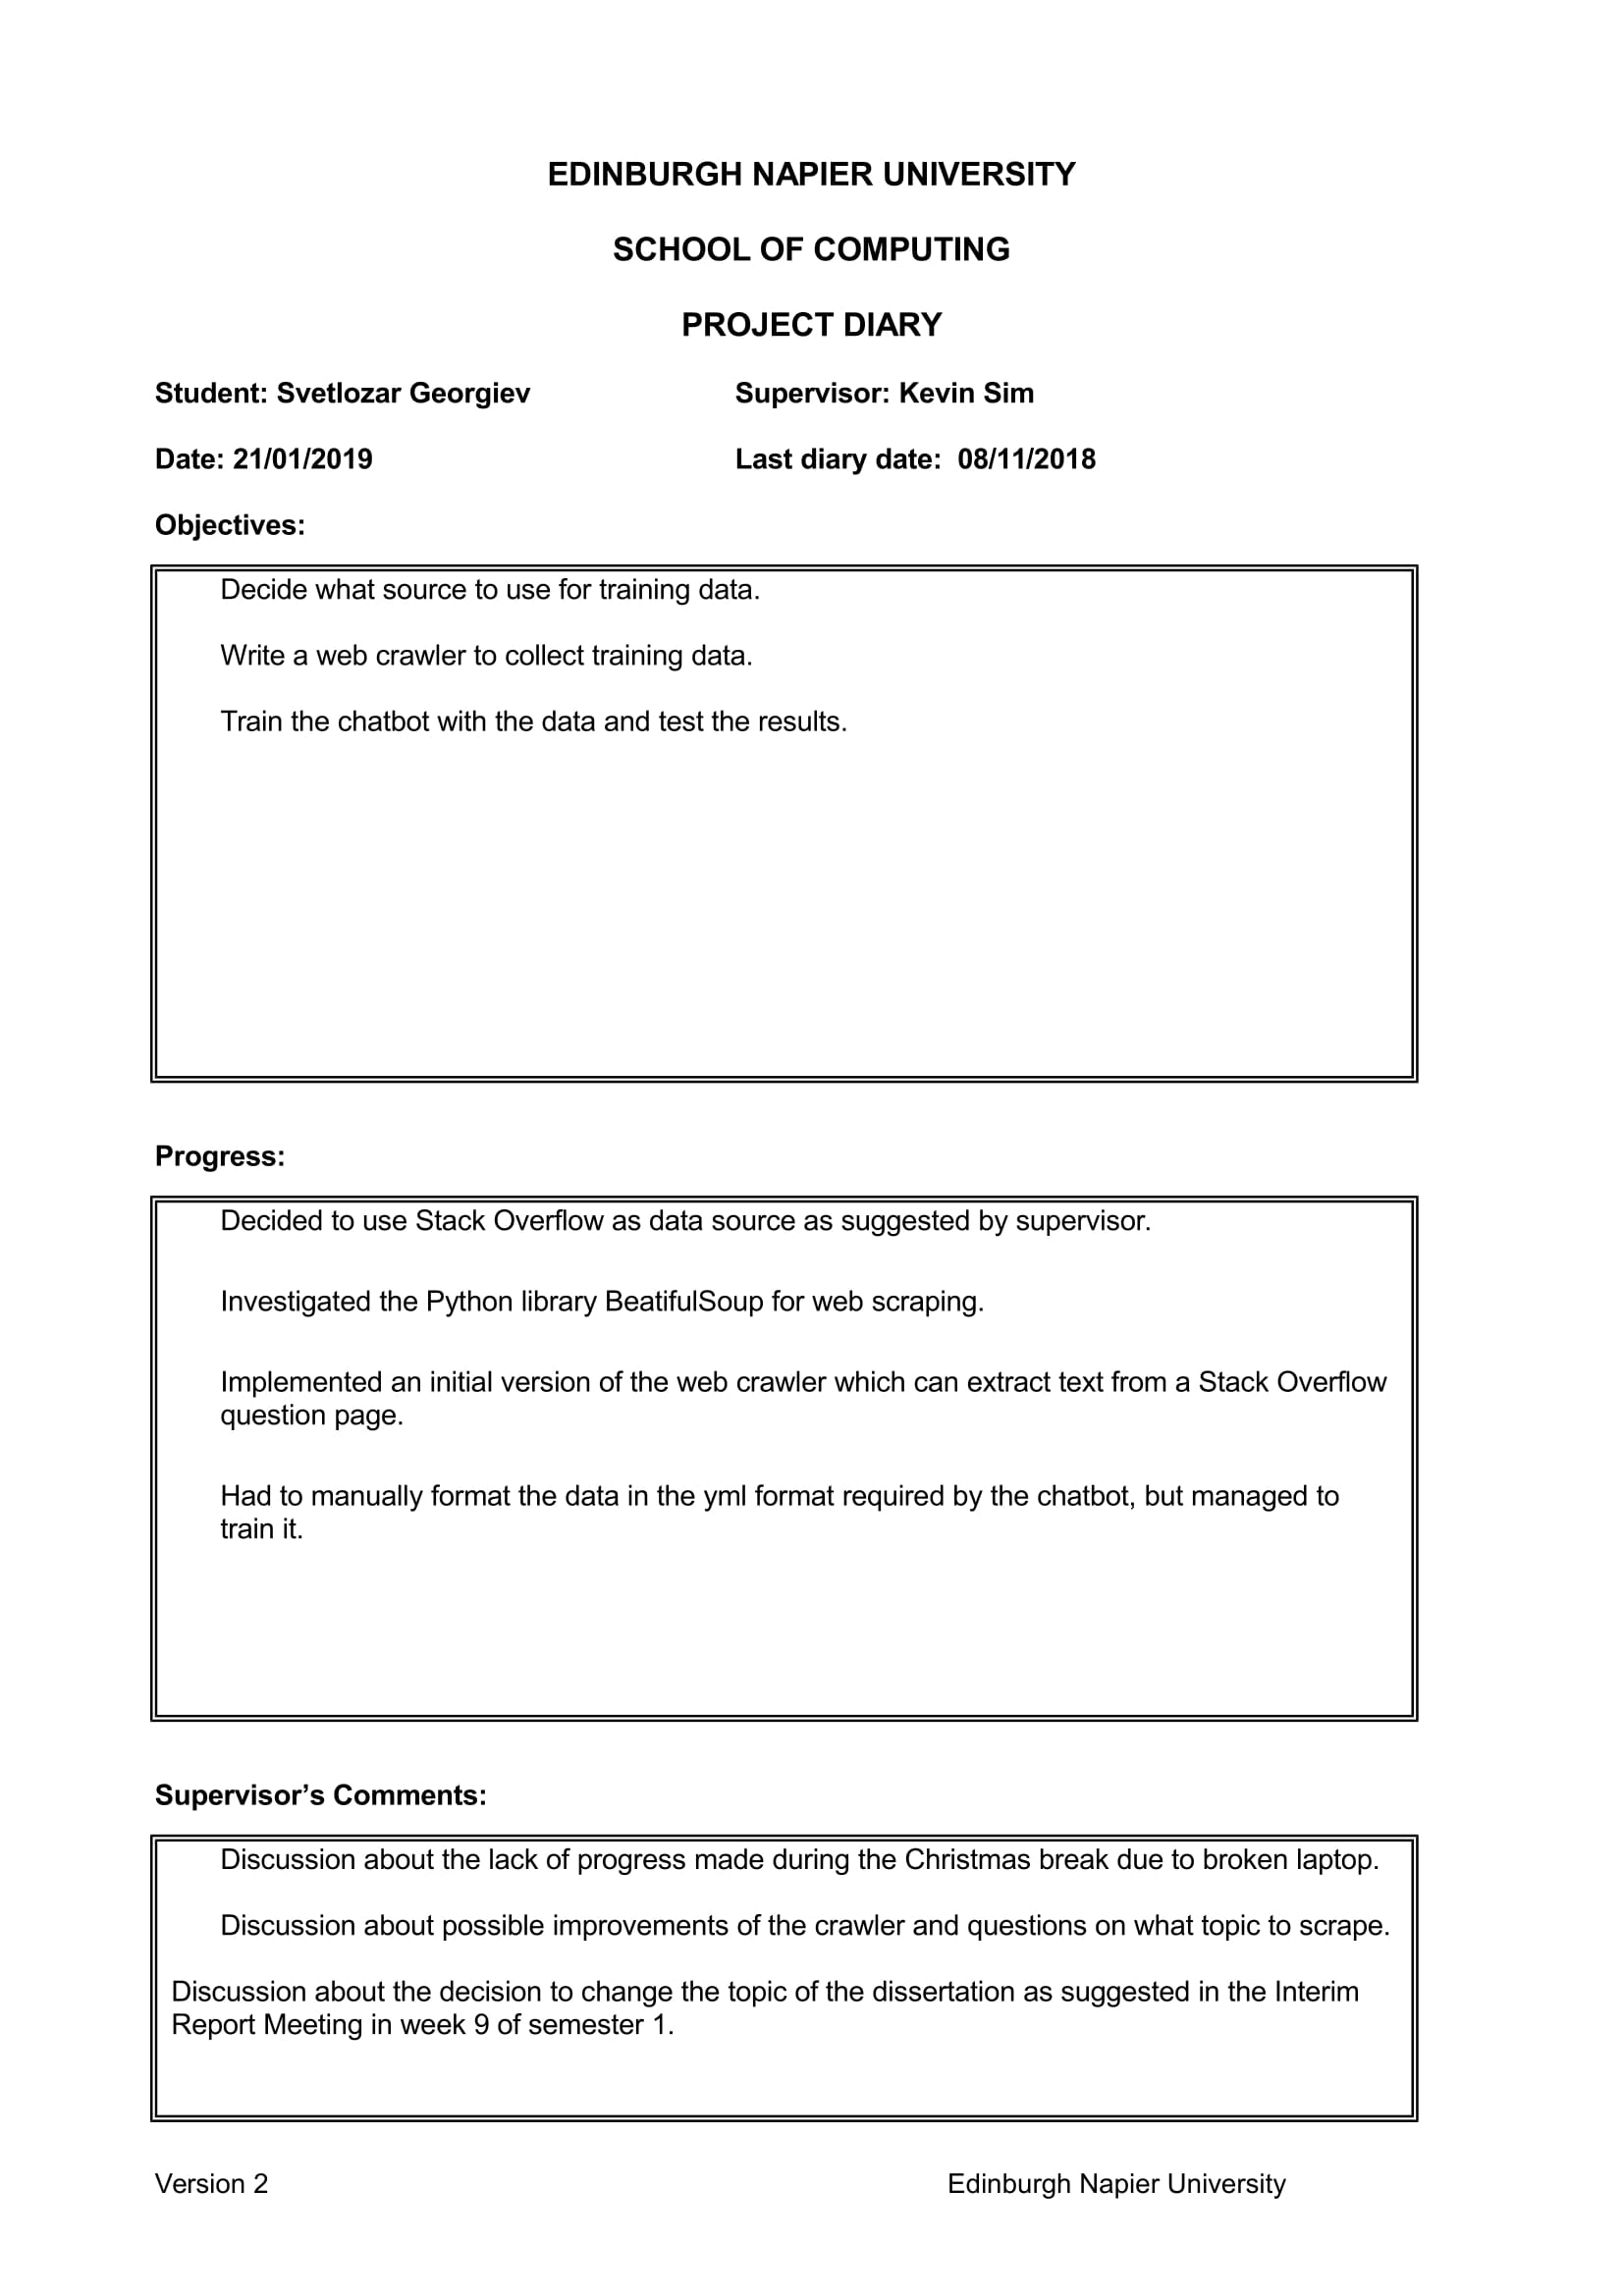
\includegraphics[width=\textwidth,height=\textheight,keepaspectratio]{s2week2.jpg} % fit images to page
\newpage
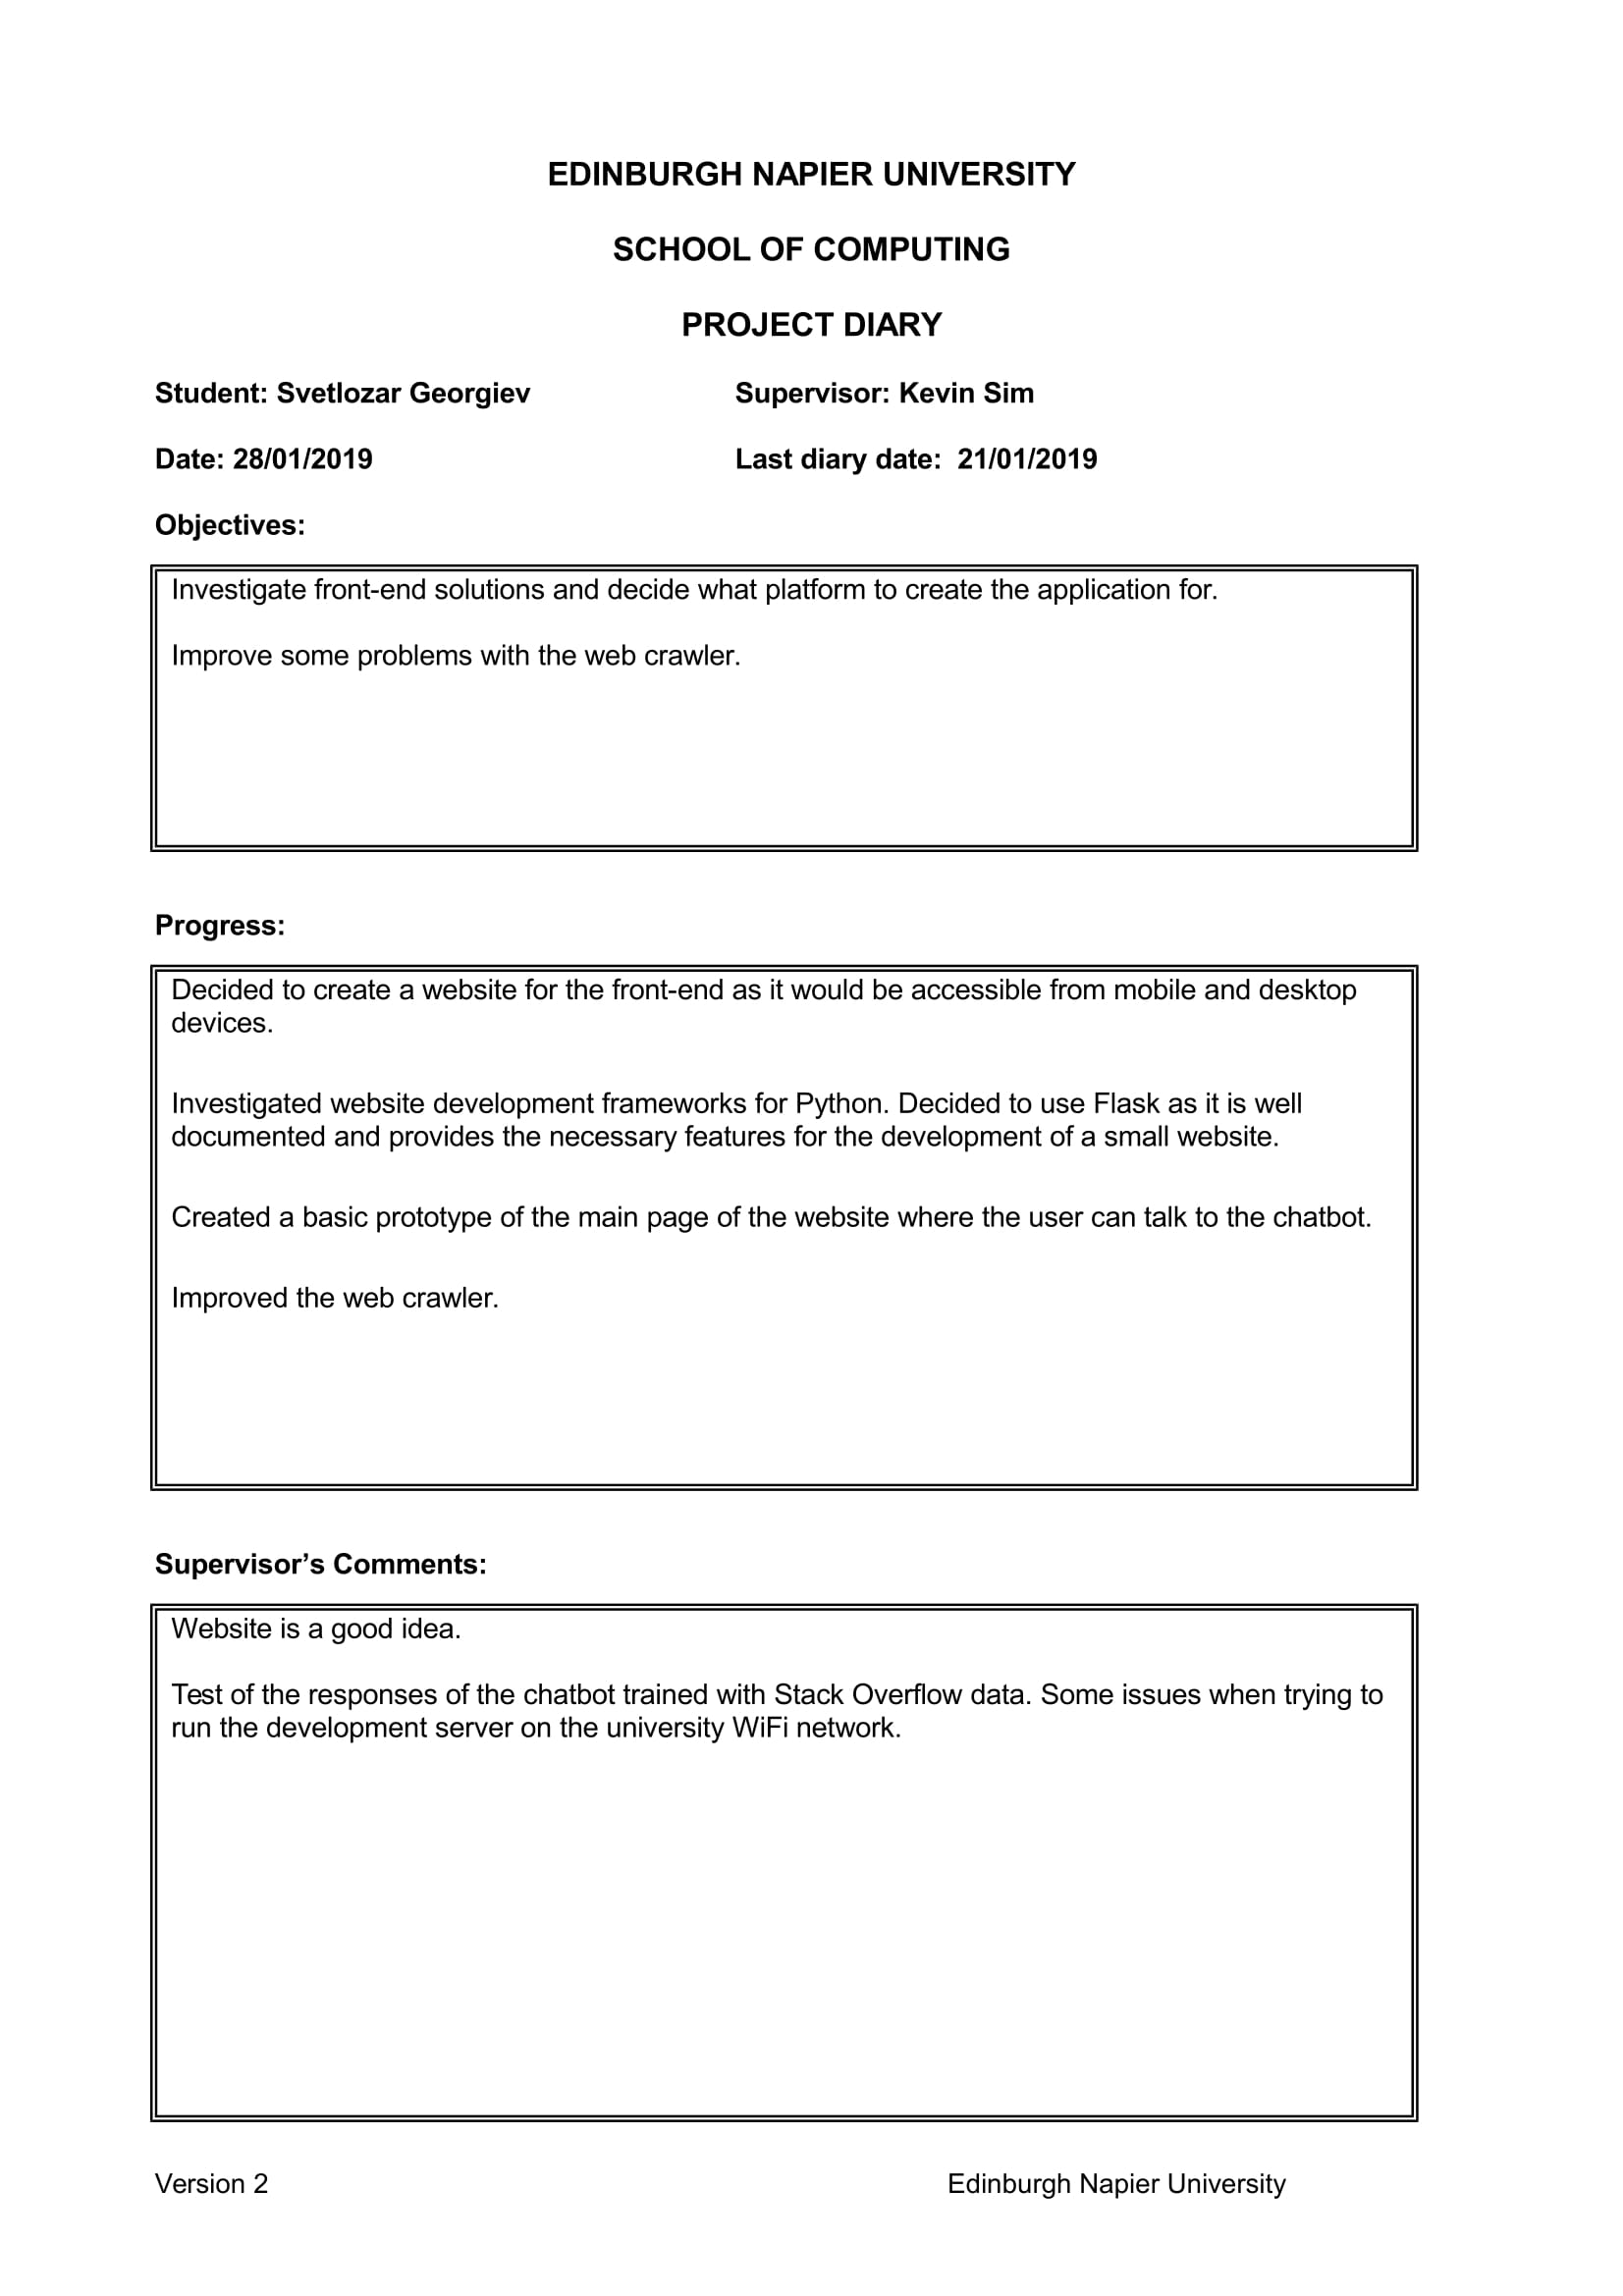
\includegraphics[width=\textwidth,height=\textheight,keepaspectratio]{s2week3.jpg}
\newpage
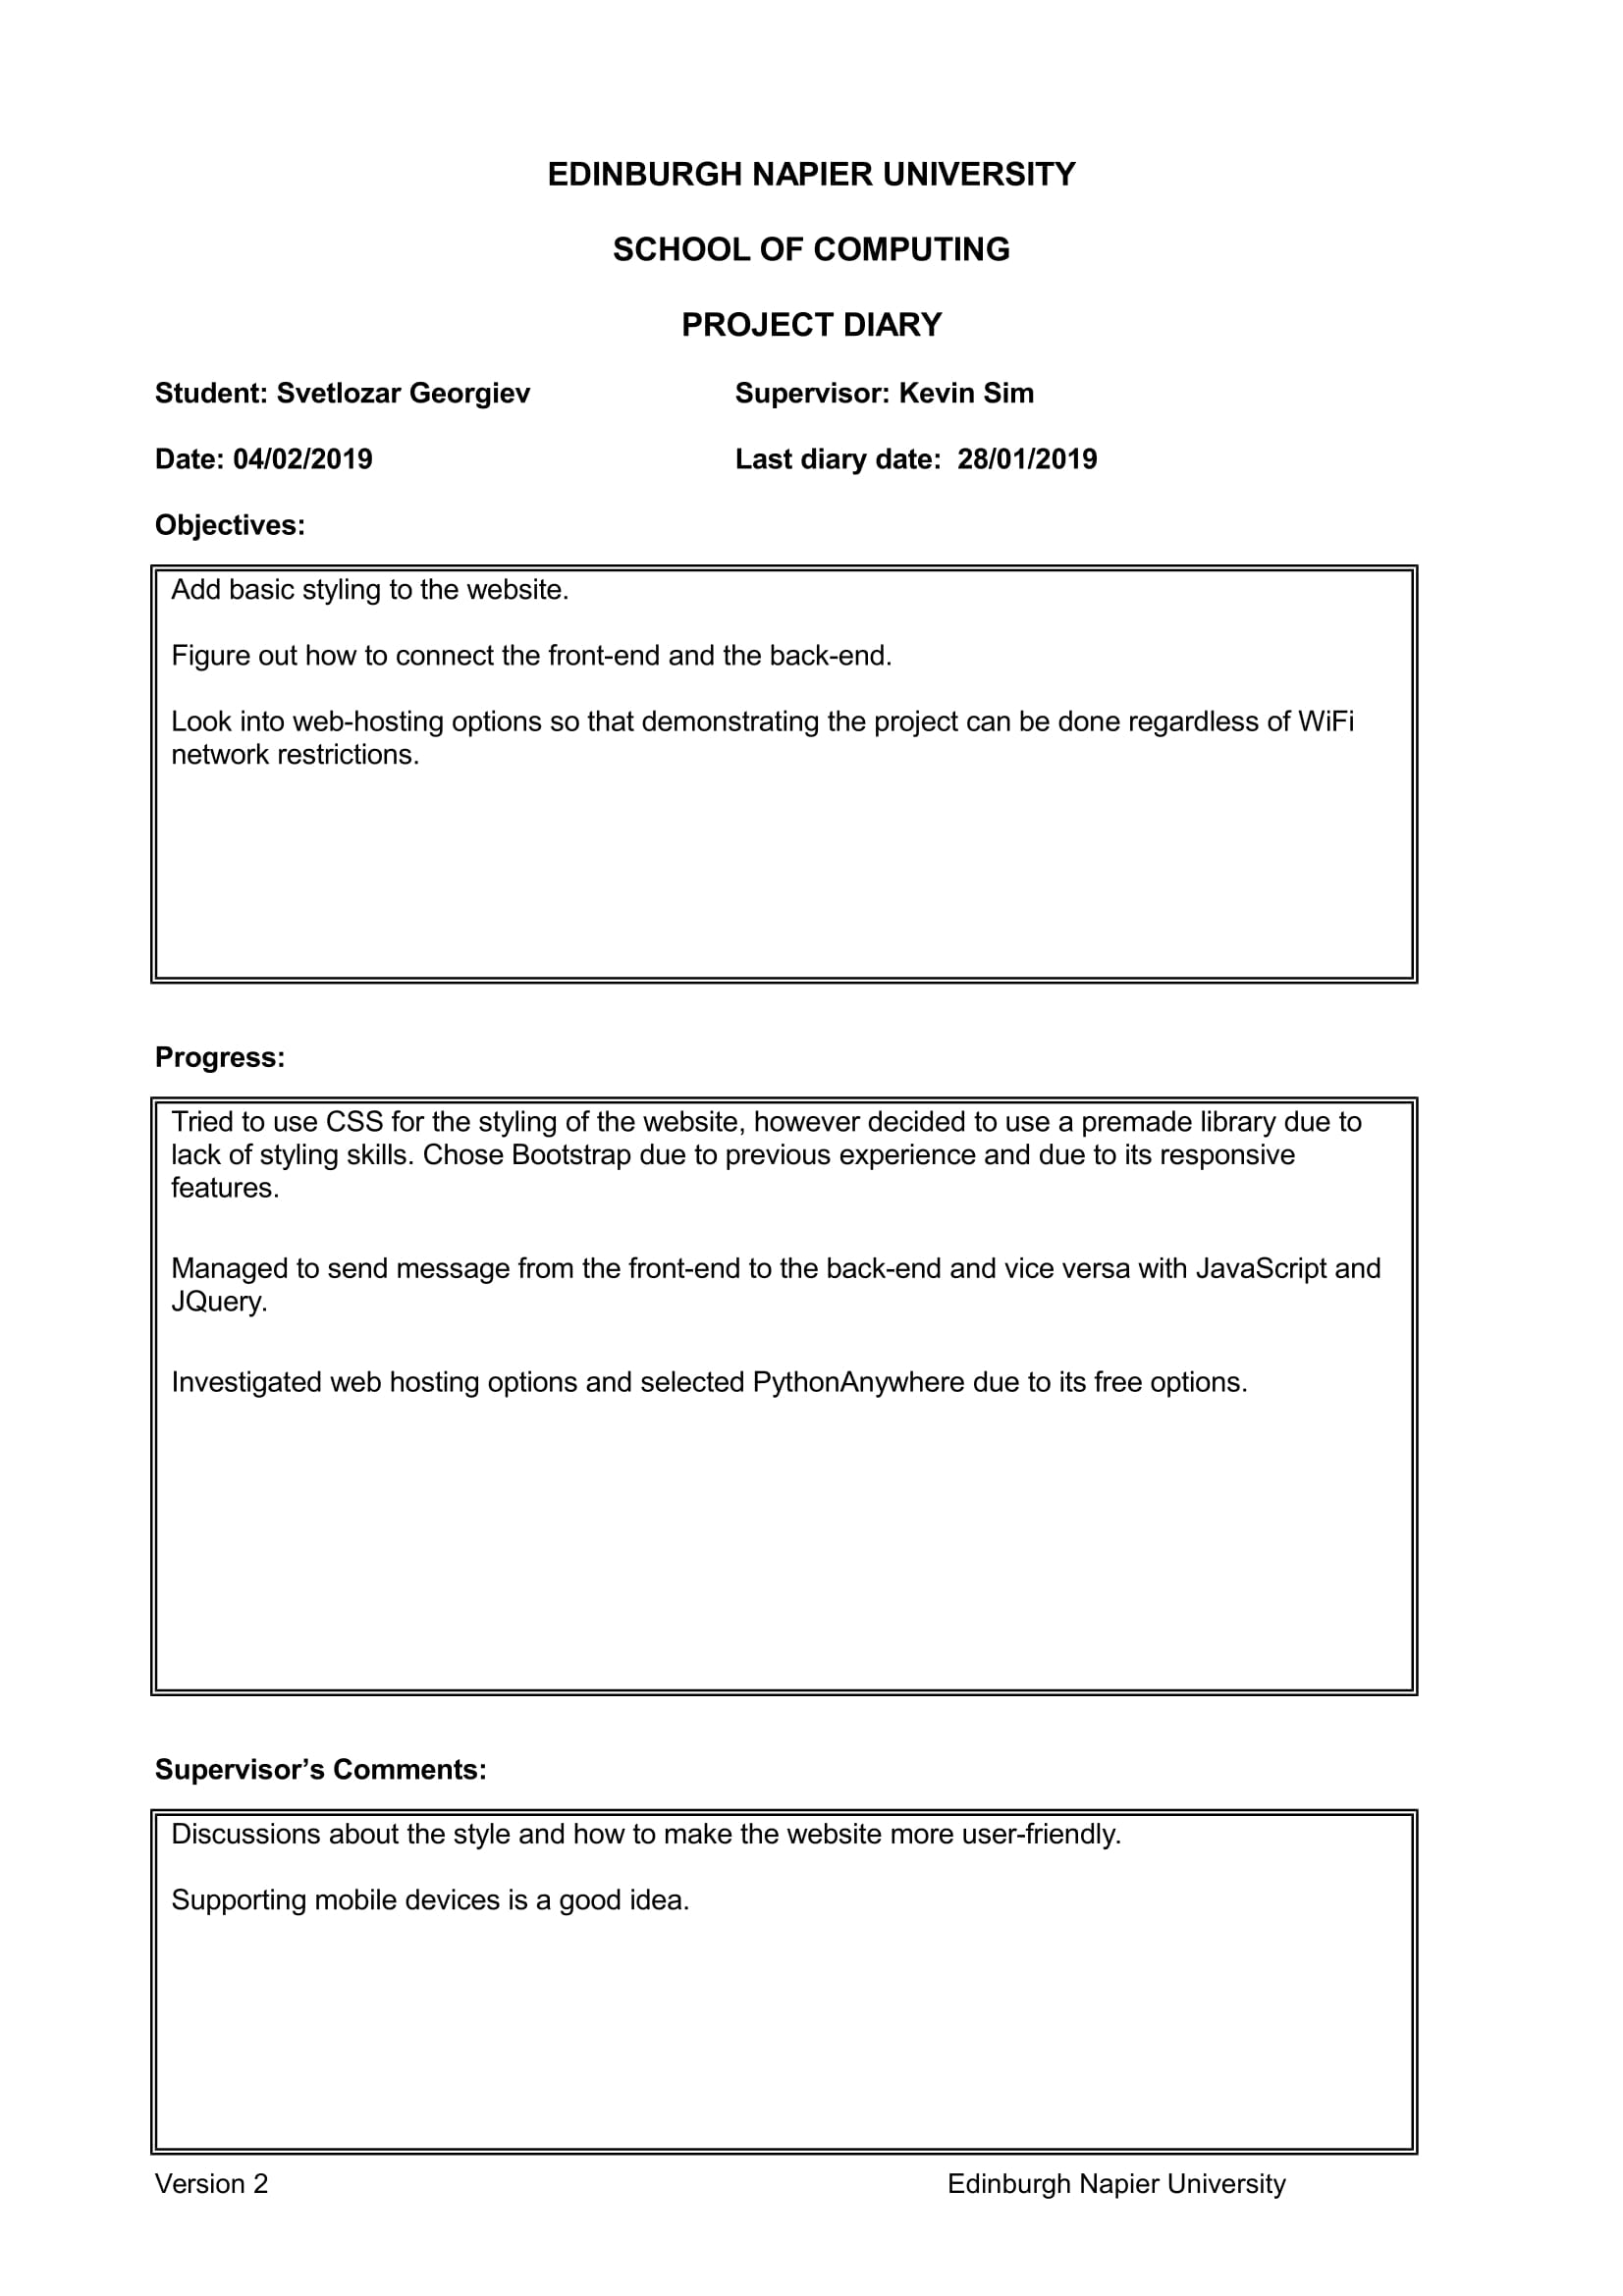
\includegraphics[width=\textwidth,height=\textheight,keepaspectratio]{s2week4.jpg}
\newpage
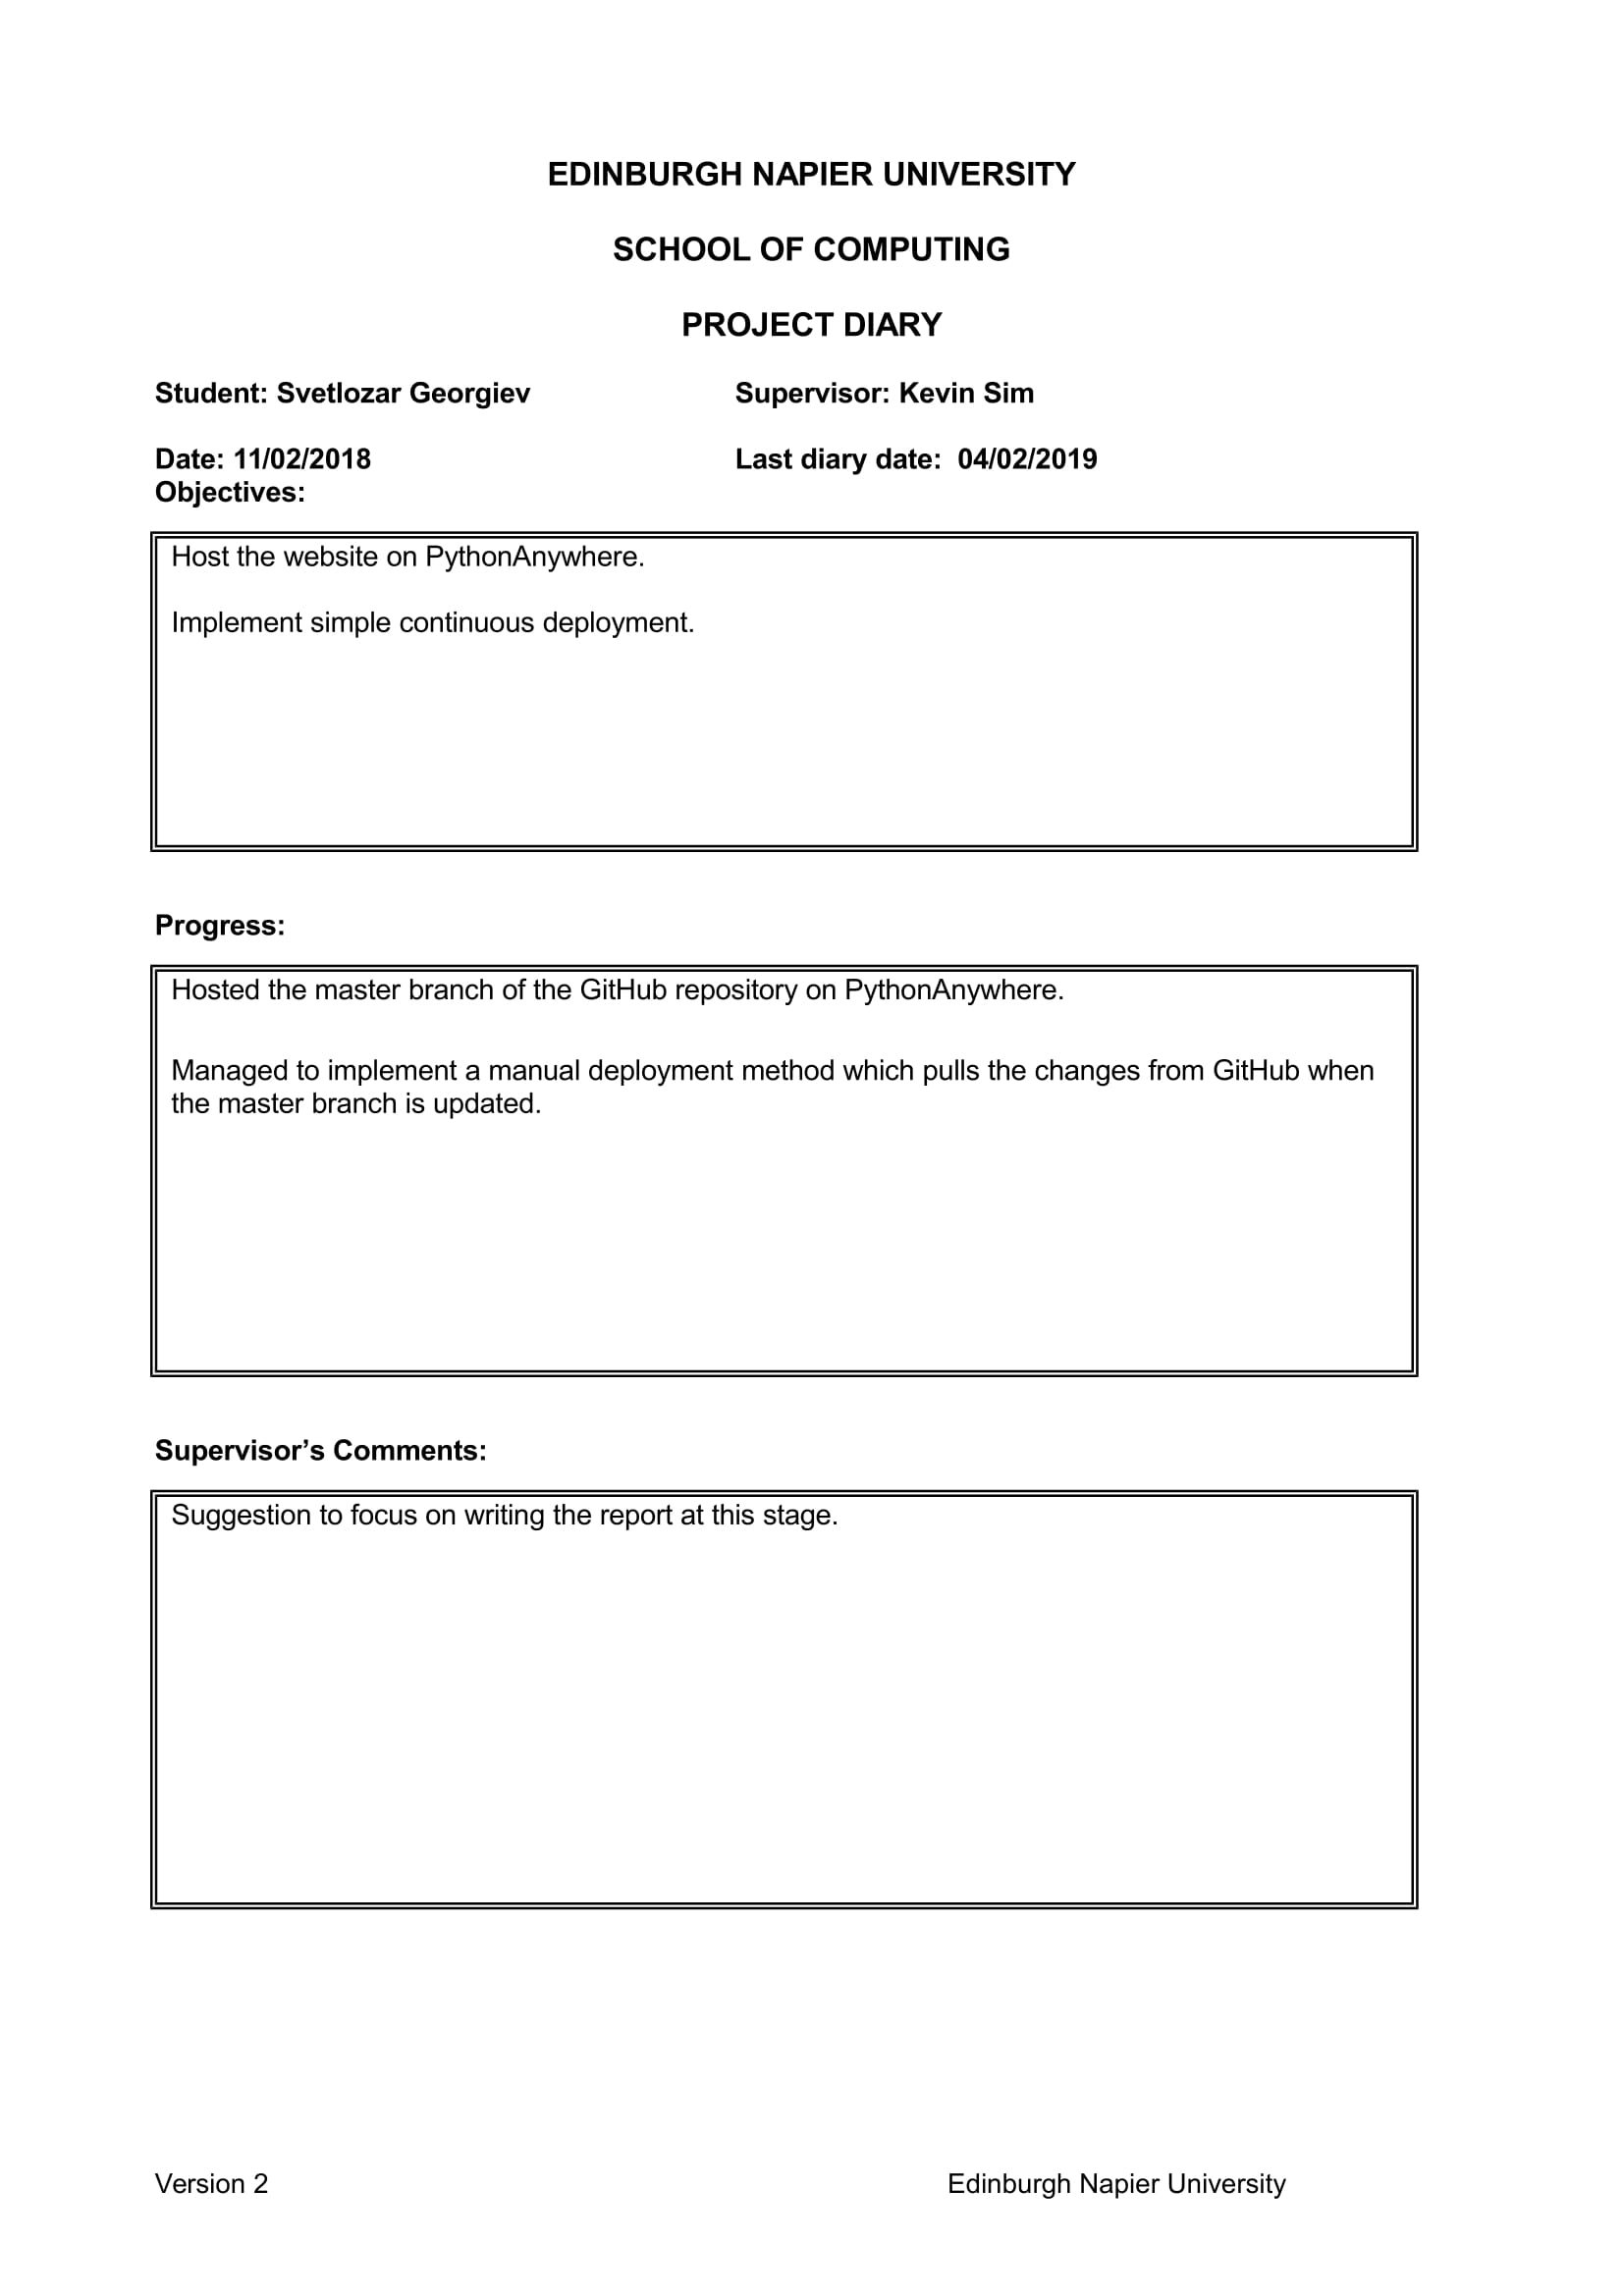
\includegraphics[width=\textwidth,height=\textheight,keepaspectratio]{s2week5.jpg}
\newpage
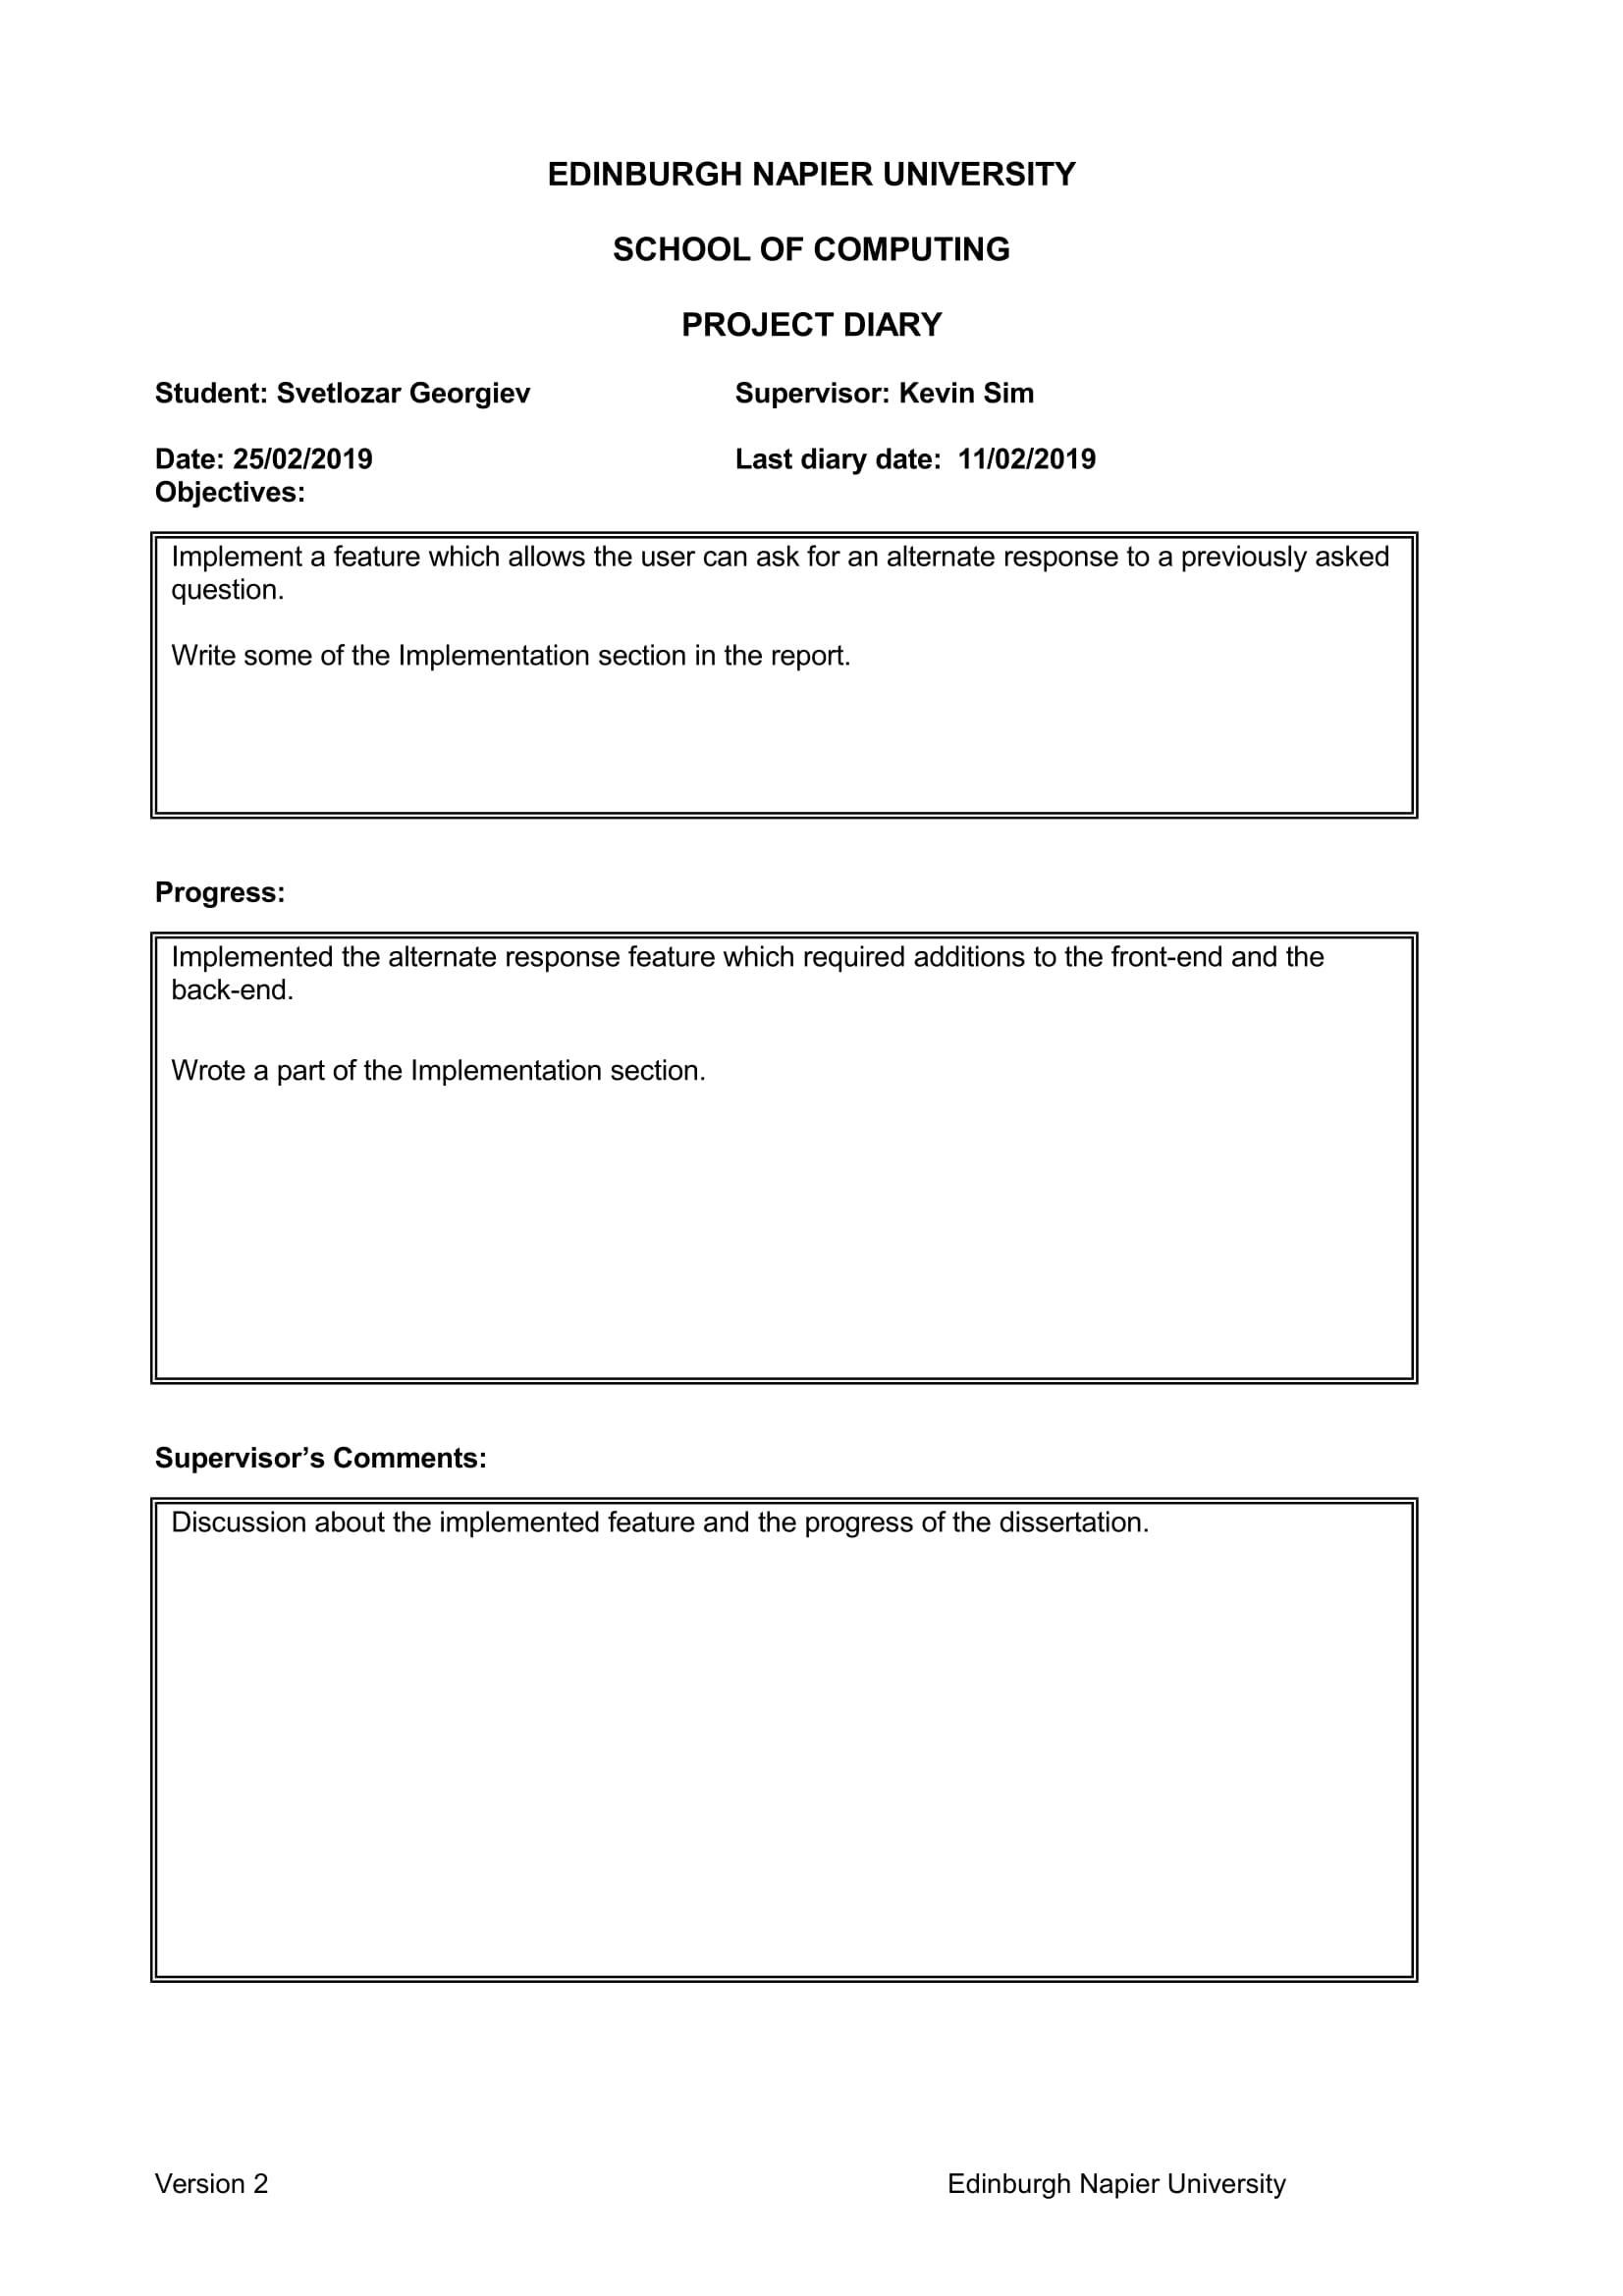
\includegraphics[width=\textwidth,height=\textheight,keepaspectratio]{s2week6.jpg}
\newpage
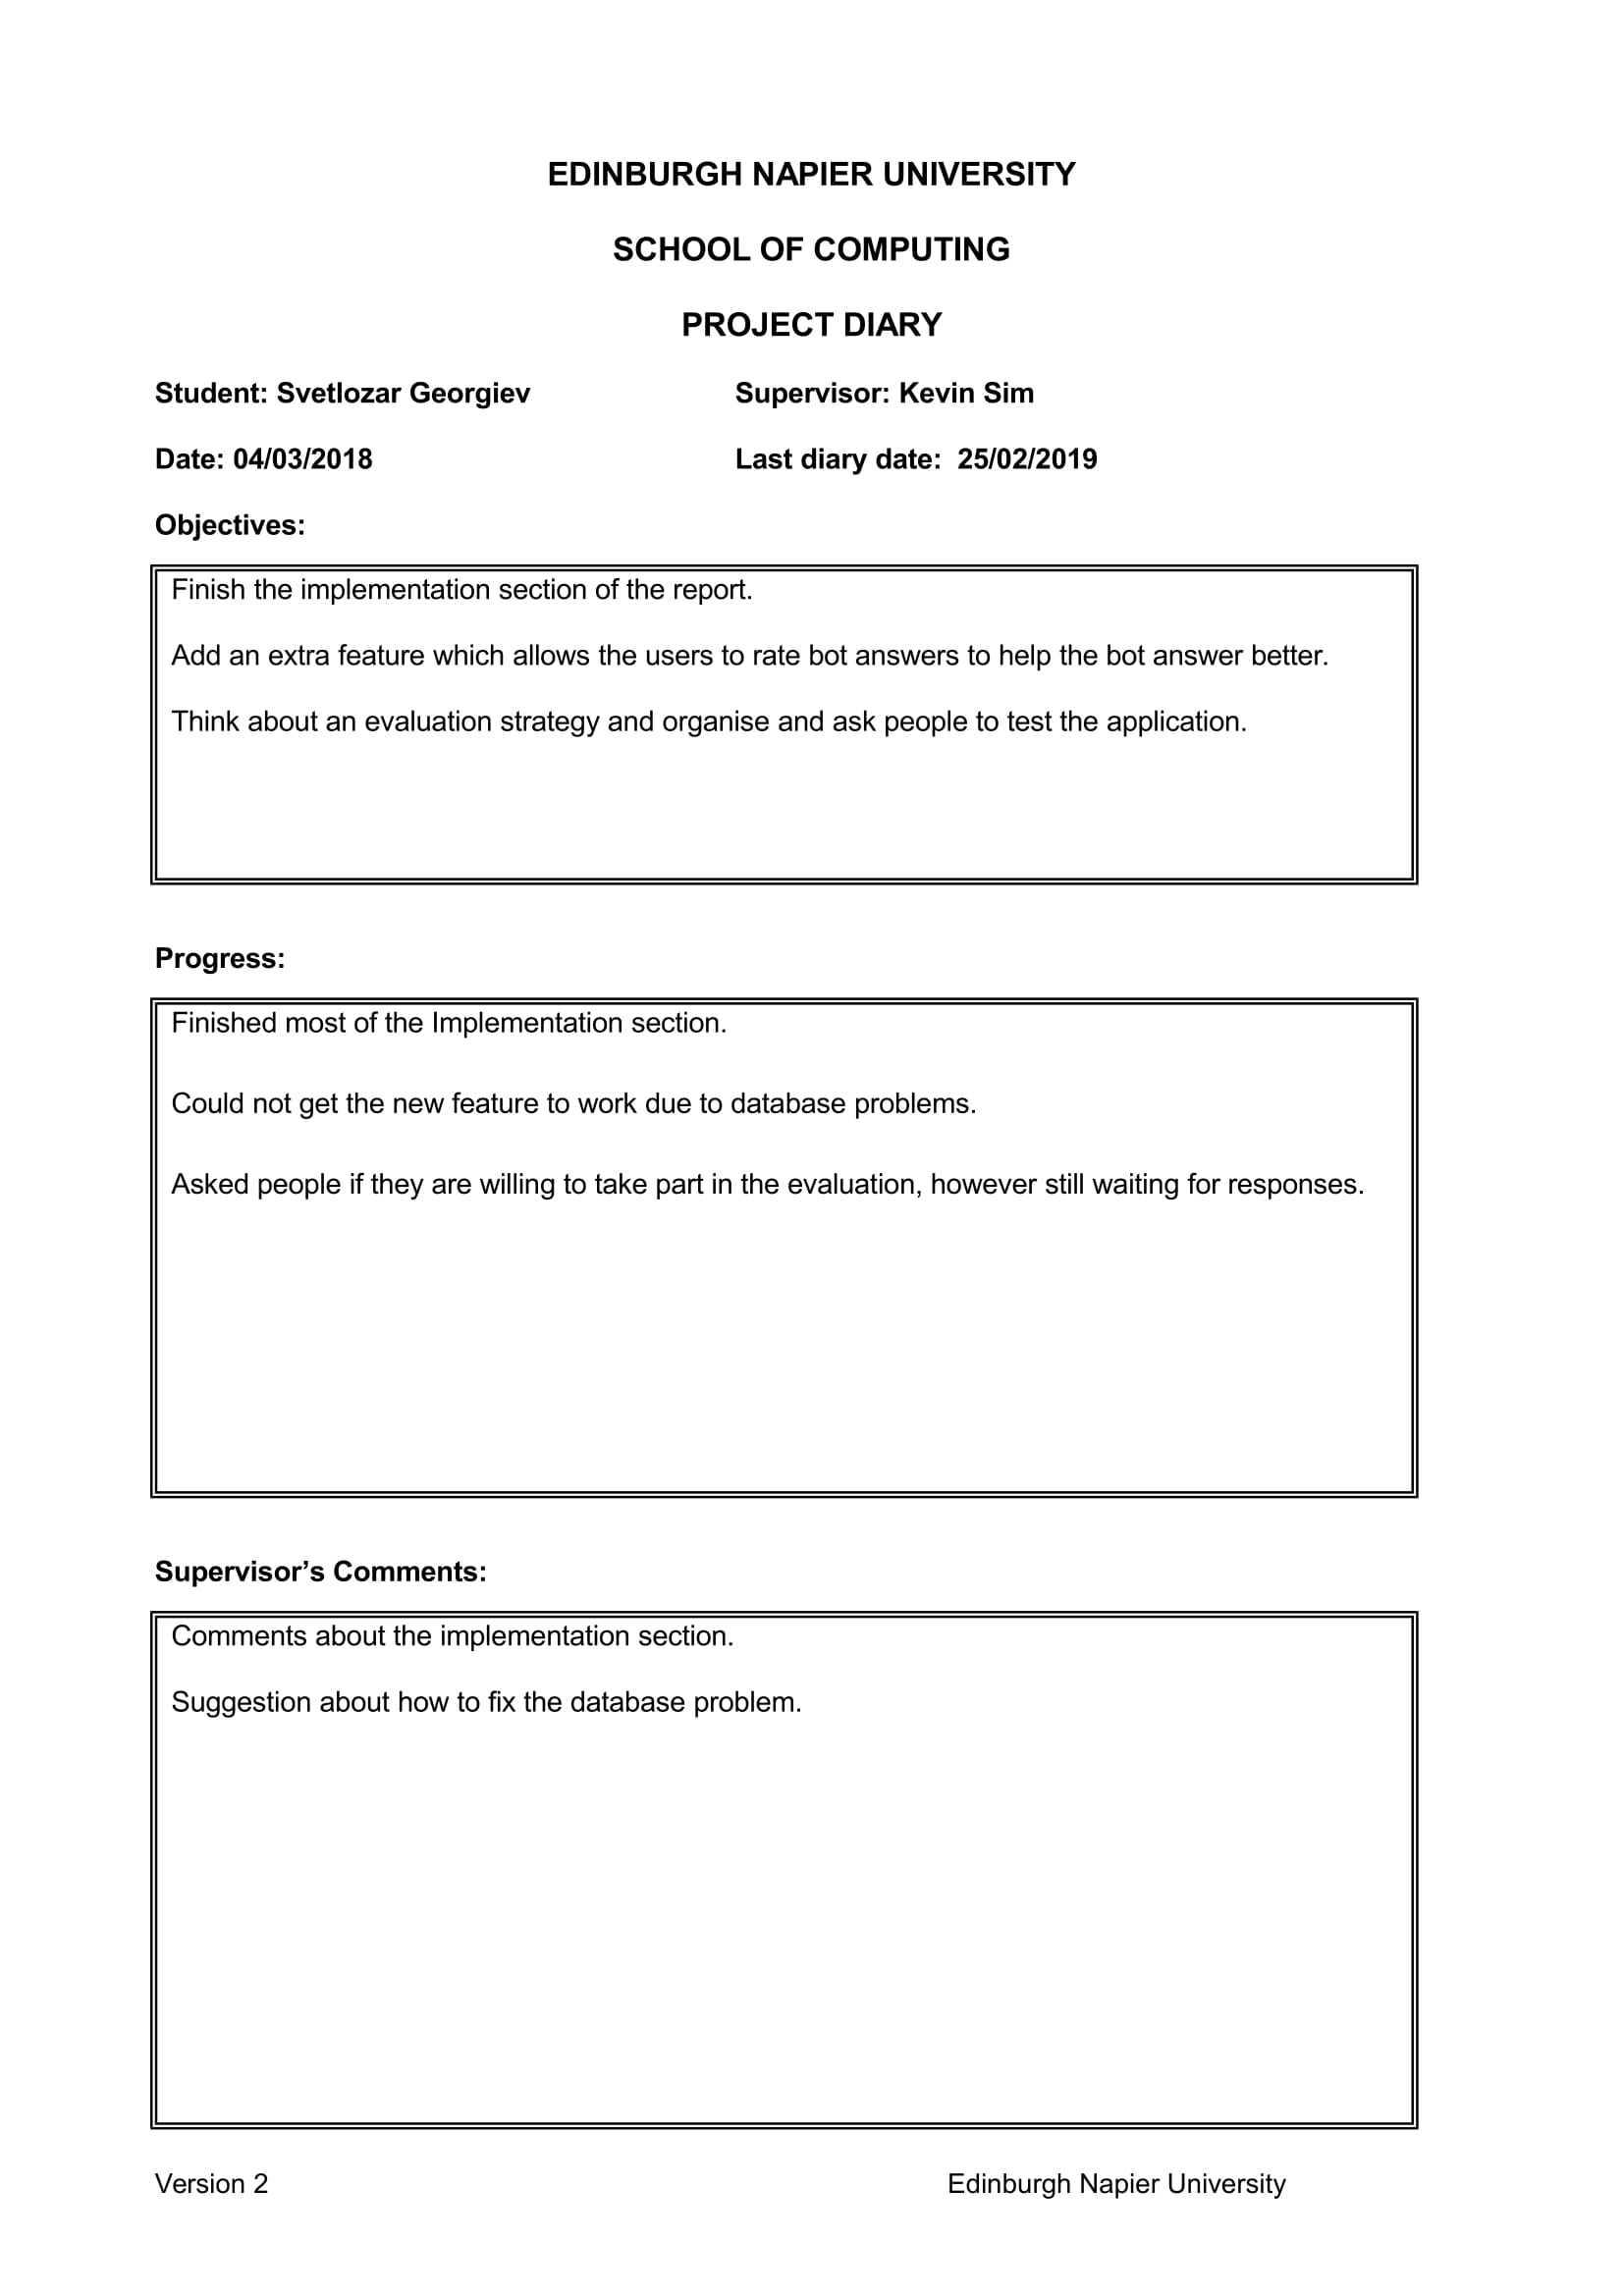
\includegraphics[width=\textwidth,height=\textheight,keepaspectratio]{s2week7.jpg}
\newpage
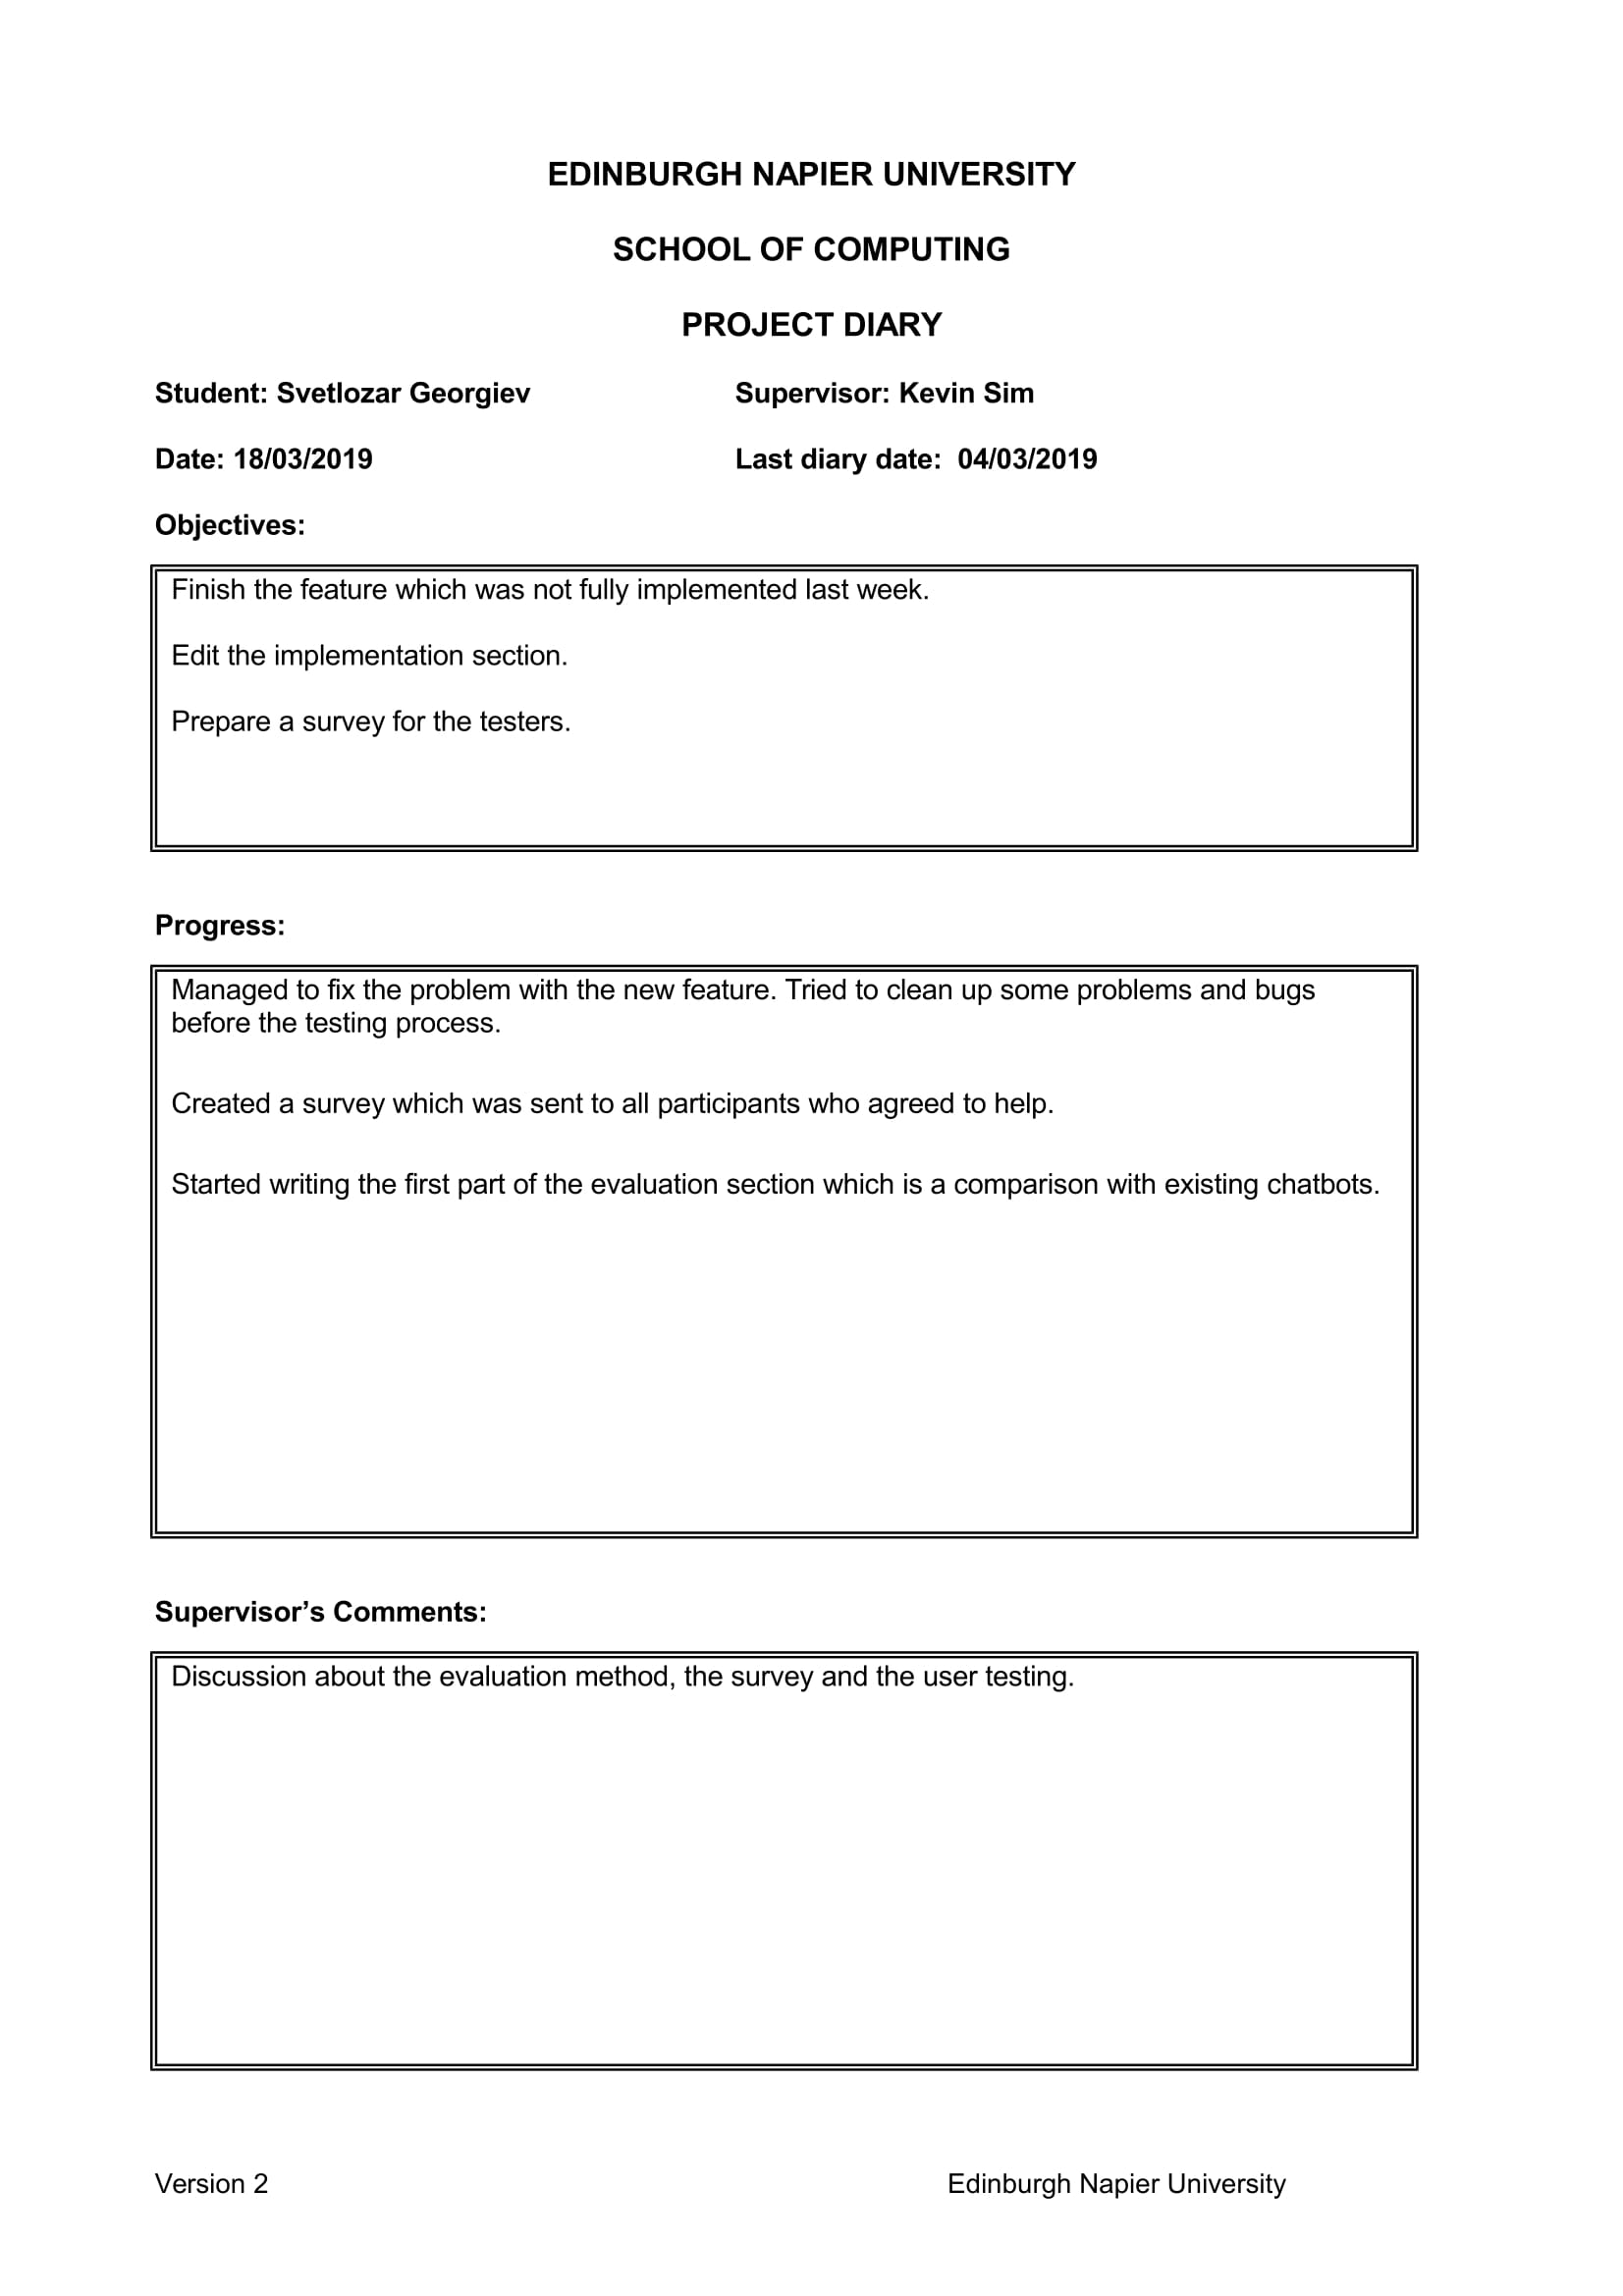
\includegraphics[width=\textwidth,height=\textheight,keepaspectratio]{s2week8.jpg}
\newpage
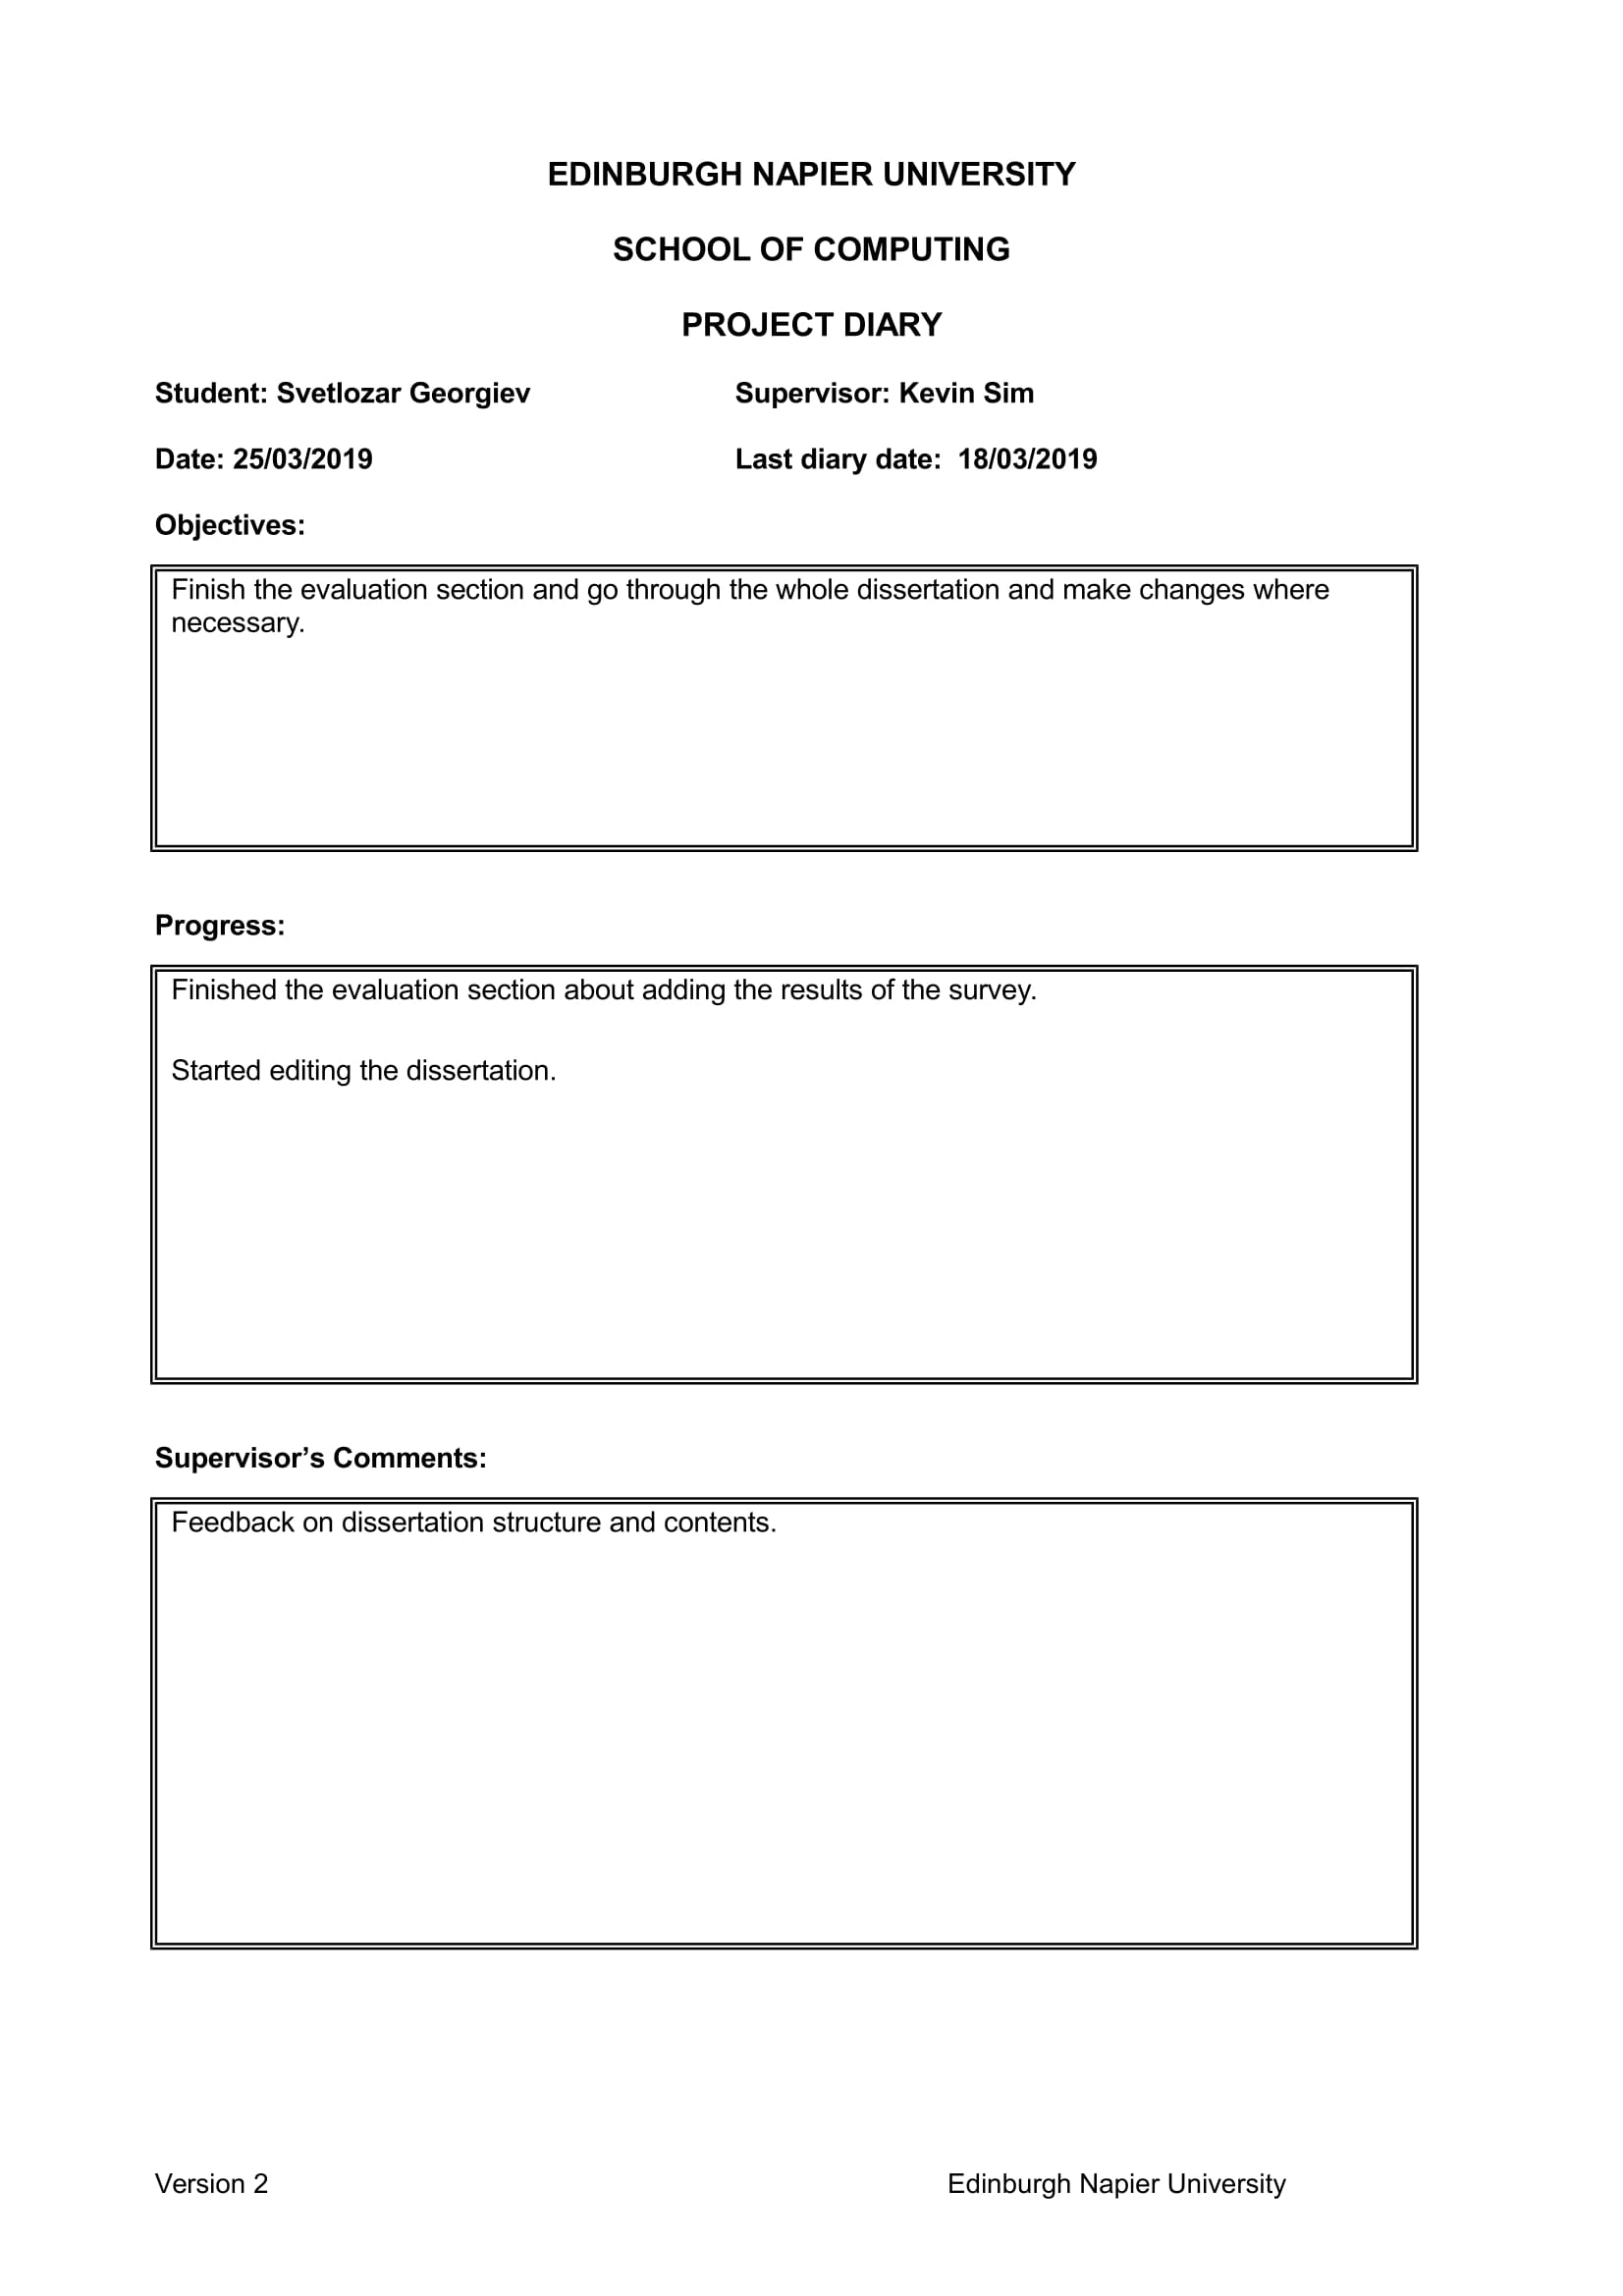
\includegraphics[width=\textwidth,height=\textheight,keepaspectratio]{s2week9.jpg}


\newpage
\section{Second Formal Review Output}\label{app:interim}
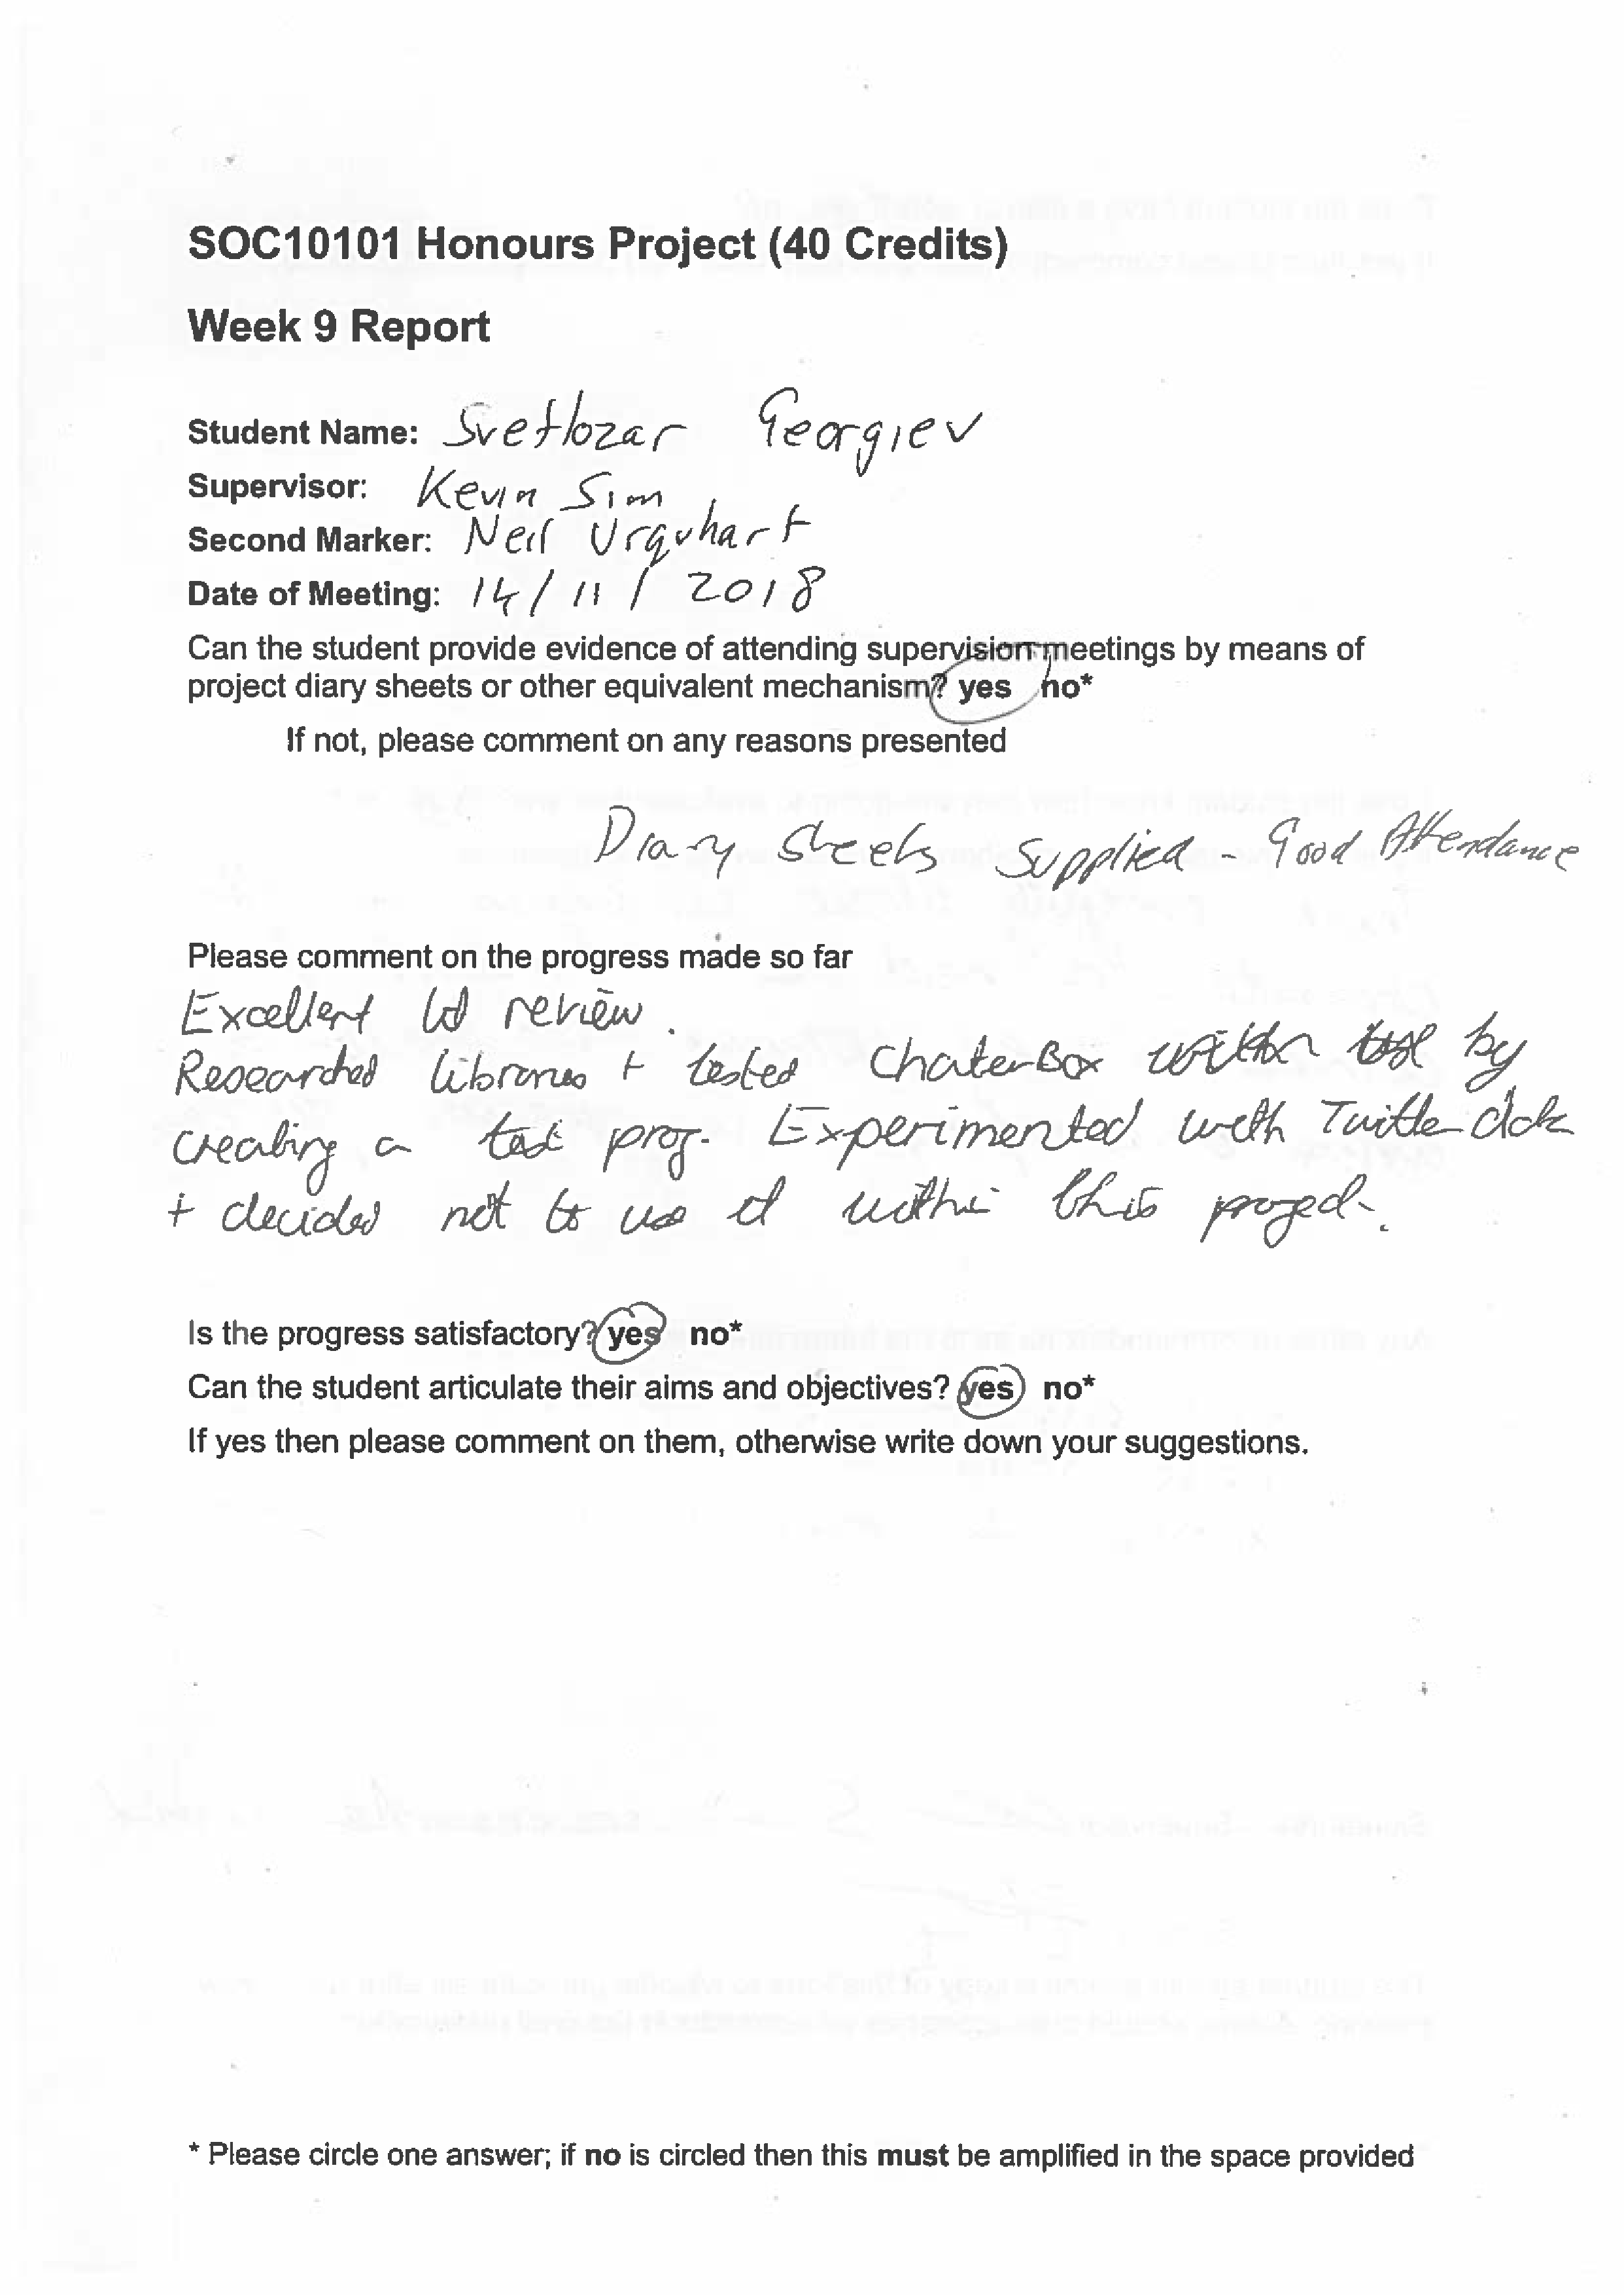
\includegraphics[width=\textwidth,height=\textheight,keepaspectratio]{interim-1.png}
\newpage
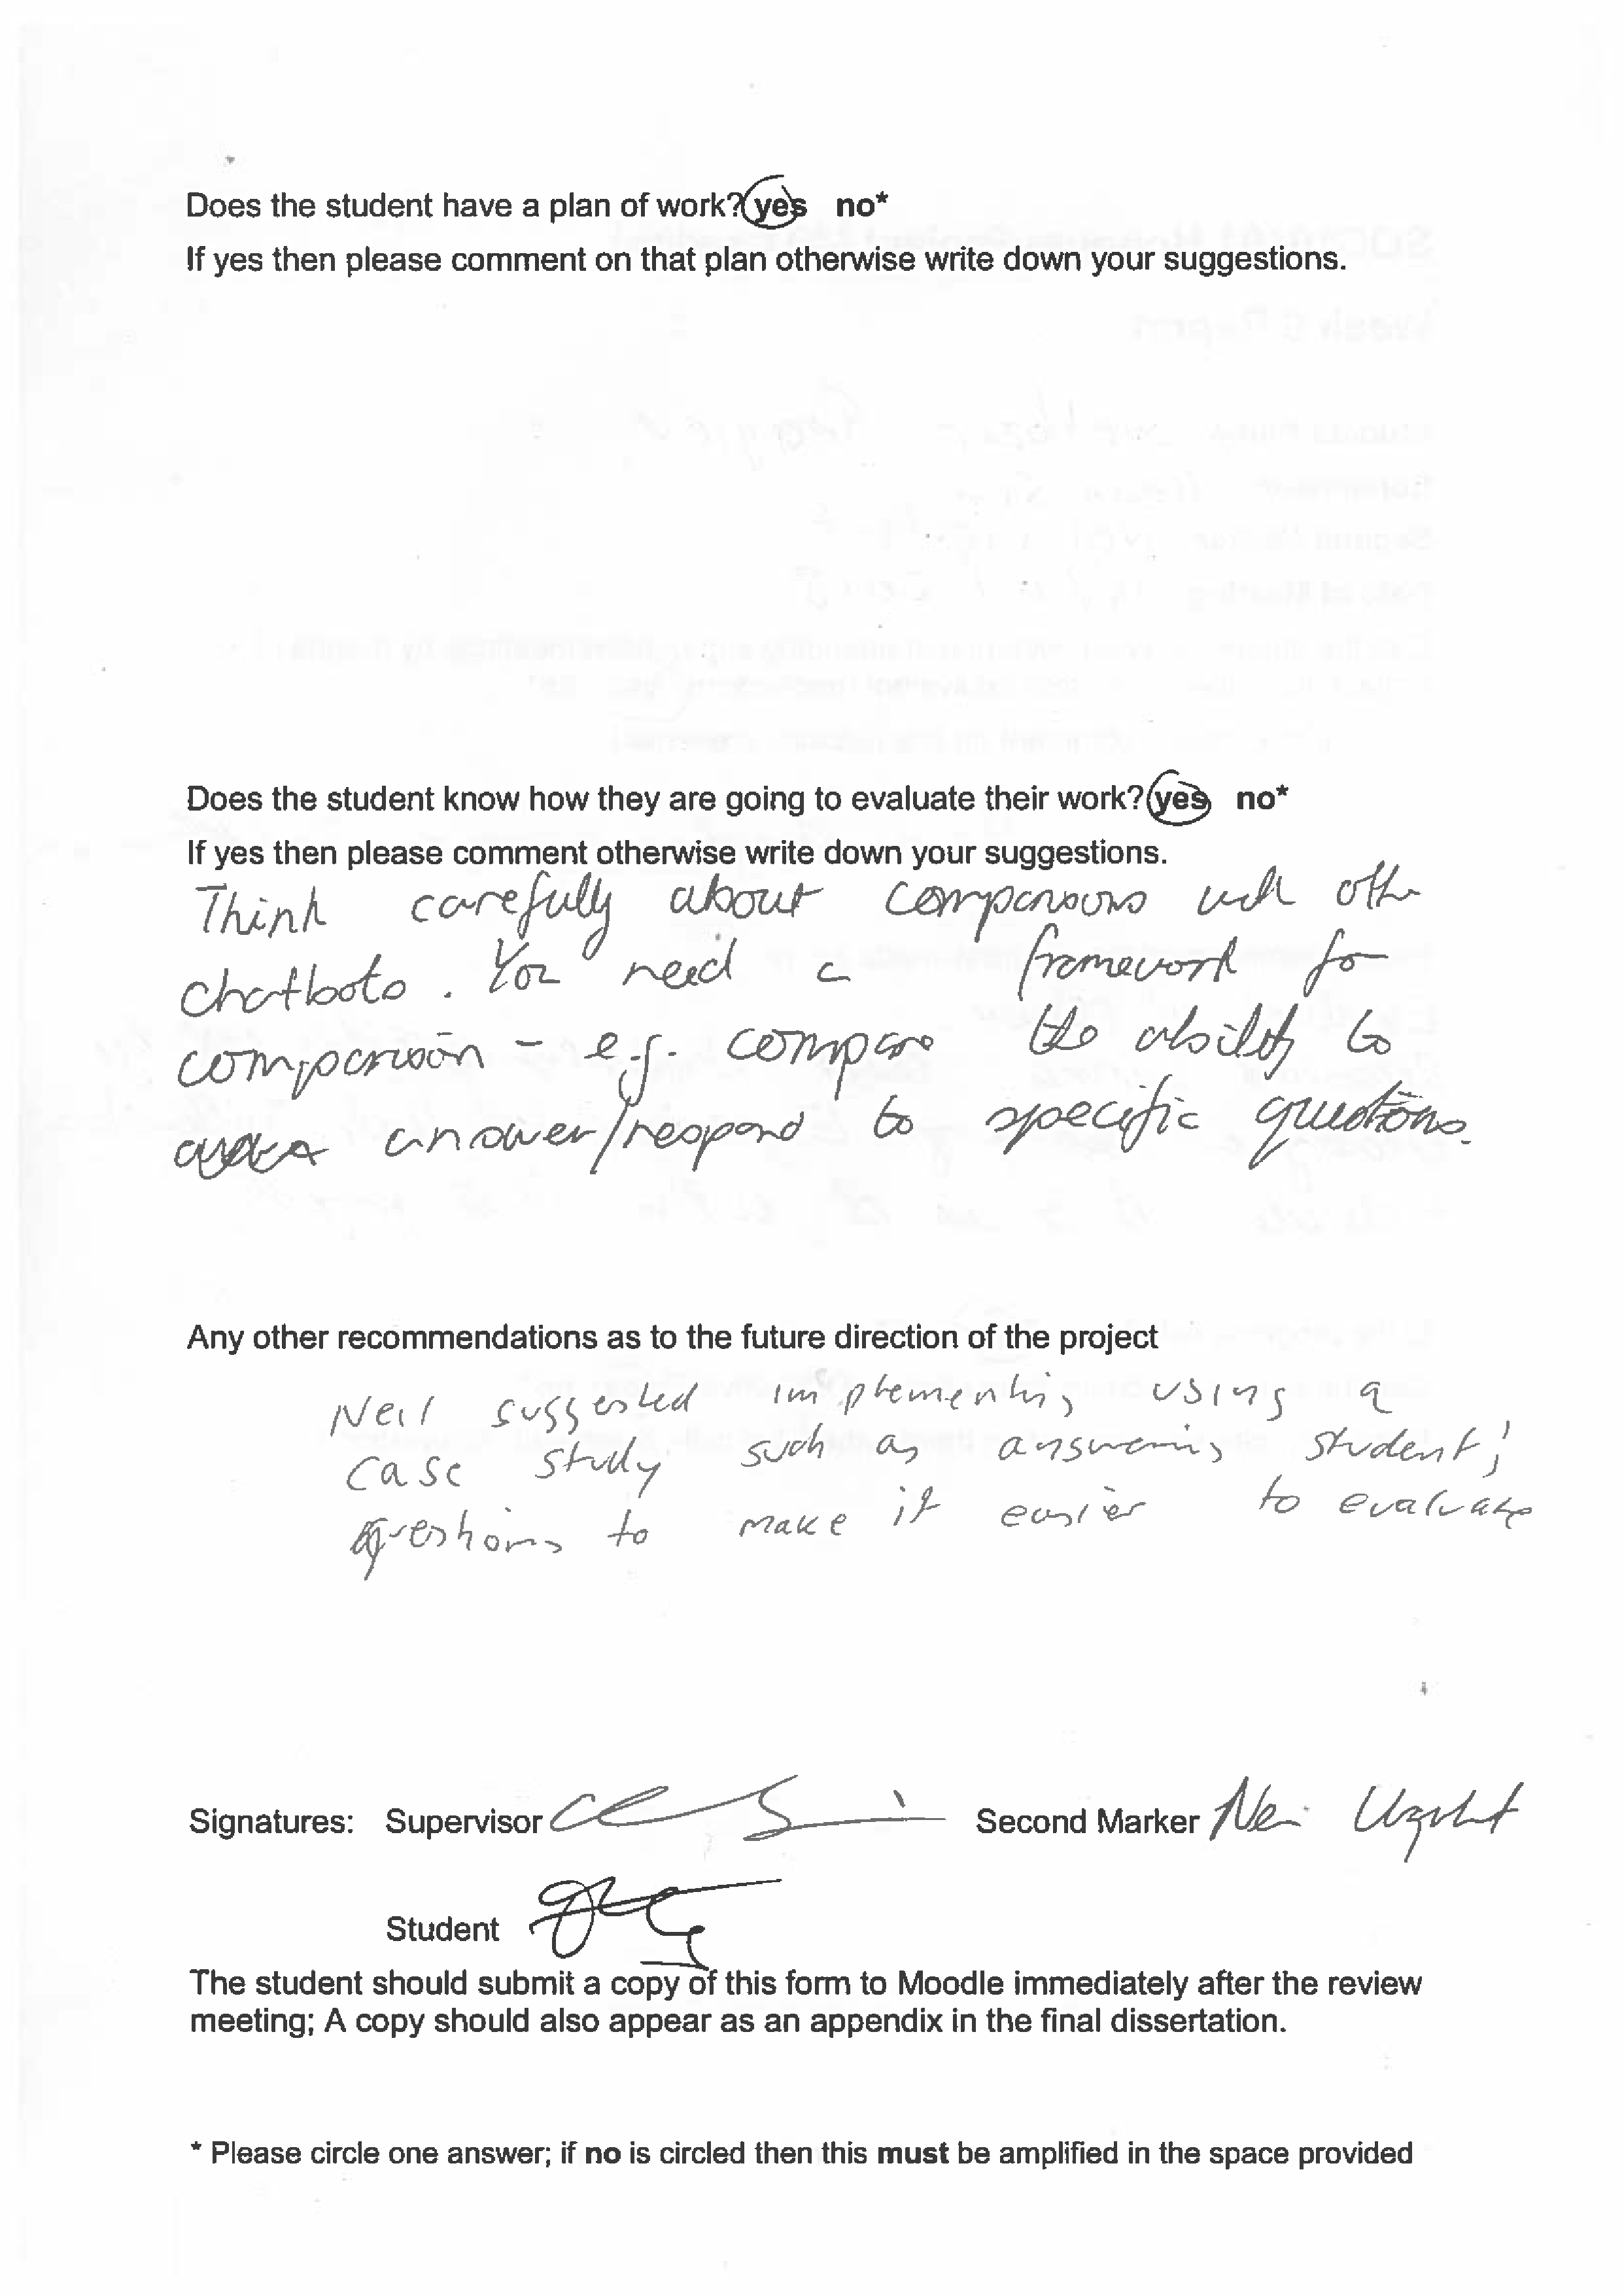
\includegraphics[width=\textwidth,height=\textheight,keepaspectratio]{interim-2.png}

\newpage
\section{Results from the First Testing Session}\label{app:sesh1}
\begin{table}[!htb]
    \centering
    \renewcommand\arraystretch{1.6}
    \caption{\captionstyle{Results from the first testing session.}}
    \label{tbl:sesh1}
    \begin{tabularx}{\textwidth}{XX}
    \toprule
    \textbf{Feedback} & \textbf{Changes made}  \\
    \midrule
    Links are not identifiable easily. & The colour of all links was changed to stand out from regular text. The style was also  changed so that they are underlined. \\
    The \enquote{help} link is not visible. & The style for this link was also changed.  Additionally, another help button was added to a menu at the top of the webpage. \\
    It would be more user-friendly to add an "alternate response" button. & An alternate response button was added to the bottom of each bot message.\\
    When the user gives negative feedback, they should be presented with an alternate  response button. & An alternate response button was added to the template for the "no" feedback button. \\
    The webpage fills the screen and  answers which are too long look like a wall of text. It is difficult to read. & The initial width of the chat box was decreased. \\
    The help message should describe the features of the application more clearly. & The help message was edited. \\
    There should be a description of the website for users who accidentally found it. & Another webpage was added which describes the purpose of the website.\\
    \bottomrule
    \end{tabularx}
\end{table}%

\newpage
\section{Survey Questions}\label{app:surveyqs}
\renewcommand\arraystretch{1.8}
\begin{longtabu} to \textwidth {cX[1]X[1]}
    \caption{\captionstyle{The questions each tester was asked in the survey and their possible answers.}} \label{tbl:sureyqs} \\
    \toprule
    \multicolumn{1}{l}{\textbf{ID}} & \multicolumn{1}{l}{\textbf{Question}} & \multicolumn{1}{l}{\textbf{Possible Answers}} \\
    \endfirsthead

    \multicolumn{3}{c}%
    {{\textbf{\tablename\ \thetable{}} \captionstyle{-- continued from previous page}}} \\
    \toprule \multicolumn{1}{l}{\textbf{ID}} & \multicolumn{1}{l}{\textbf{Question}} & \multicolumn{1}{l}{\textbf{Possible Answers}} \\ \hline
    \endhead

    \hline \multicolumn{3}{r}{{\small{Continued on next page}}} \\ \bottomrule 
    \endfoot

    \bottomrule
    \endlastfoot
    
    \midrule
    \rownumber & What is your overall programming knowledge? & Beginner/Intermediate/Advanced \\
%    3 & How often do you use search engines to search for information related to programming? & Daily/Weekly/Monthly/Less often\\
%    4 & How often do you use Stack Overflow? & Daily/Weekly/Monthly/Less often \\
    \rownumber & The user interface is easy to understand and use. & Scale from "Strongly Agree" to "Strongly Disagree" \\
    \rownumber & The user interface is visually pleasing. & Scale from "Strongly Agree" to "Strongly Disagree" \\
    \rownumber & I was able to understand how to use all the features of the application, i.e. asking for a \textbf{regular response}, asking for an \textbf{alternate response}, and providing \textbf{feedback} for a bot response. & Scale from "Strongly Agree" to "Strongly Disagree" \\
    \rownumber & I was able to use the \textbf{alternate response feature} to receive an alternate answer to a question I asked. & Scale from "Strongly Agree" to "Strongly Disagree".\\
    \rownumber & I was able to use the \textbf{feedback feature} to give feedback on an answer the chatbot gave me. & Scale from "Strongly Agree" to "Strongly Disagree" \\
    \rownumber & Appropriate error messages are shown (e.g. when there is no user input). & Scale from "Strongly Agree" to "Strongly Disagree" \\
    \rownumber & The chatbot answered my question(s) quickly. & Scale from "Strongly Agree" to "Strongly Disagree" \\
    \rownumber & The chatbot response(s) were coherent and answered my question(s) accurately. & Scale from "Strongly Agree" to "Strongly Disagree" \\
    \rownumber & I am overall satisfied with the functionality of the application. & Scale from "Strongly Agree" to "Strongly Disagree" \\
%    14 & I prefer using the application on a... & Mobile Device/Desktop Device \\
    \rownumber & Any additional feedback? & Text input field where the user can write their additional feedback.\\
\end{longtabu}

%\newpage
%\section{Survey Results}\label{app:surveyresults}


\newpage
\section{Web Crawling Program}\label{app:crawler}
\lstinputlisting[caption={[\captionstyle{The source code of the second web crawling program.}]\captionstyle{The source code of the second web crawling program created for data collection from the ISO C\texttt{++} website.}}]{cppfaqcrawler.py}

\end{appendices}

\end{document}
